\documentclass[a4paper]{book}
\usepackage{makeidx}
\usepackage{natbib}
\usepackage{graphicx}
\usepackage{multicol}
\usepackage{float}
\usepackage{listings}
\usepackage{color}
\usepackage{ifthen}
\usepackage[table]{xcolor}
\usepackage{textcomp}
\usepackage{alltt}
\usepackage{ifpdf}
\ifpdf
\usepackage[pdftex,
            pagebackref=true,
            colorlinks=true,
            linkcolor=blue,
            unicode
           ]{hyperref}
\else
\usepackage[ps2pdf,
            pagebackref=true,
            colorlinks=true,
            linkcolor=blue,
            unicode
           ]{hyperref}
\usepackage{pspicture}
\fi
\usepackage[utf8]{inputenc}
\usepackage{mathptmx}
\usepackage[scaled=.90]{helvet}
\usepackage{courier}
\usepackage{sectsty}
\usepackage[titles]{tocloft}
\usepackage{doxygen}
\lstset{language=C++,inputencoding=utf8,basicstyle=\footnotesize,breaklines=true,breakatwhitespace=true,tabsize=8,numbers=left }
\makeindex
\setcounter{tocdepth}{3}
\renewcommand{\footrulewidth}{0.4pt}
\renewcommand{\familydefault}{\sfdefault}
\hfuzz=15pt
\setlength{\emergencystretch}{15pt}
\hbadness=750
\tolerance=750
\begin{document}
\hypersetup{pageanchor=false,citecolor=blue}
\begin{titlepage}
\vspace*{7cm}
\begin{center}
{\Large \-Smart\-Led }\\
\vspace*{1cm}
{\large \-Generated by Doxygen 1.7.6.1}\\
\vspace*{0.5cm}
{\small Tue Apr 12 2016 16:22:59}\\
\end{center}
\end{titlepage}
\clearemptydoublepage
\pagenumbering{roman}
\tableofcontents
\clearemptydoublepage
\pagenumbering{arabic}
\hypersetup{pageanchor=true,citecolor=blue}
\chapter{\-Module \-Index}
\section{\-Modules}
\-Here is a list of all modules\-:\begin{DoxyCompactList}
\item \contentsline{section}{\-G\-U\-I\-: \-A\-P\-P \-Group}{\pageref{group___g_u_i}}{}
\item \contentsline{section}{\-Manage\-: \-A\-P\-P \-Group}{\pageref{group___m_a_n_a_g_e}}{}
\item \contentsline{section}{main\-: \-A\-P\-P \-Group}{\pageref{group___m_a_i_n}}{}
\item \contentsline{section}{\-Widget\-: \-A\-P\-P \-Group}{\pageref{group___w_i_d_g_e_t}}{}
\item \contentsline{section}{\-Power\-: \-A\-P\-P \-Group}{\pageref{group___p_o_w_e_r}}{}
\item \contentsline{section}{\-Protocol\-: \-A\-P\-P \-Group}{\pageref{group___p_r_o_t_o_c_o_l}}{}
\item \contentsline{section}{\-Task\-: \-A\-P\-P \-Group}{\pageref{group___t_a_s_k}}{}
\item \contentsline{section}{\-Bsp\-: \-B\-S\-P \-Group}{\pageref{group___b_s_p}}{}
\item \contentsline{section}{\-Bsp\-Battery\-: \-B\-S\-P \-Group}{\pageref{group___b_e_t_t_e_r_y}}{}
\item \contentsline{section}{\-Bsp\-Ble\-: \-B\-S\-P \-Group}{\pageref{group___b_l_e}}{}
\item \contentsline{section}{\-Bsp\-Key\-: \-B\-S\-P \-Group}{\pageref{group___k_e_y}}{}
\item \contentsline{section}{\-Bsp\-Led\-: \-B\-S\-P \-Group}{\pageref{group___l_e_d}}{}
\item \contentsline{section}{\-Bsp\-Oled\-: \-B\-S\-P \-Group}{\pageref{group___o_l_e_d}}{}
\item \contentsline{section}{\-Bsp\-Rtc\-: \-B\-S\-P \-Group}{\pageref{group___r_t_c}}{}
\item \contentsline{section}{\-Bsp\-Temp\-: \-B\-S\-P \-Group}{\pageref{group___t_e_m_p}}{}
\item \contentsline{section}{\-Bsp\-Timer\-: \-B\-S\-P \-Group}{\pageref{group___t_i_m_e_r}}{}
\item \contentsline{section}{stm32\-\_\-adc\-: \-C\-P\-U \-Group}{\pageref{group___a_d_c}}{}
\item \contentsline{section}{stm32\-\_\-i2c\-: \-C\-P\-U \-Group}{\pageref{group___i2_c}}{}
\item \contentsline{section}{stm32\-\_\-pwm\-: \-C\-P\-U \-Group}{\pageref{group___p_w_m}}{}
\item \contentsline{section}{stm32\-\_\-rcc\-: \-C\-P\-U \-Group}{\pageref{group___r_c_c}}{}
\item \contentsline{section}{stm32\-\_\-spi\-: \-C\-P\-U \-Group}{\pageref{group___s_p_i}}{}
\item \contentsline{section}{stm32\-\_\-systick\-: \-C\-P\-U \-Group}{\pageref{group___s_y_s_t_i_c_k}}{}
\item \contentsline{section}{stm32\-\_\-uart\-: \-C\-P\-U \-Group}{\pageref{group___u_a_r_t}}{}
\end{DoxyCompactList}

\chapter{\-Data \-Structure \-Index}
\section{\-Data \-Structures}
\-Here are the data structures with brief descriptions\-:\begin{DoxyCompactList}
\item\contentsline{section}{\hyperlink{struct_s_t_r___b_a_t_t_e_r_y}{\-S\-T\-R\-\_\-\-B\-A\-T\-T\-E\-R\-Y} \\*电池信息结构体 }{\pageref{struct_s_t_r___b_a_t_t_e_r_y}}{}
\item\contentsline{section}{\hyperlink{struct_s_t_r___ble}{\-S\-T\-R\-\_\-\-Ble} \\*低功耗蓝牙结构体 }{\pageref{struct_s_t_r___ble}}{}
\item\contentsline{section}{\hyperlink{struct_s_t_r___ble_msg}{\-S\-T\-R\-\_\-\-Ble\-Msg} \\*发送缓冲区中报文数量 }{\pageref{struct_s_t_r___ble_msg}}{}
\item\contentsline{section}{\hyperlink{struct_s_t_r___clock}{\-S\-T\-R\-\_\-\-Clock} \\*时钟控件结构体 }{\pageref{struct_s_t_r___clock}}{}
\item\contentsline{section}{\hyperlink{struct_s_t_r___color}{\-S\-T\-R\-\_\-\-Color} \\*\-L\-E\-D彩灯模式结构体 }{\pageref{struct_s_t_r___color}}{}
\item\contentsline{section}{\hyperlink{struct_s_t_r___gui}{\-S\-T\-R\-\_\-\-Gui} \\*\-G\-U\-I显示结构体 }{\pageref{struct_s_t_r___gui}}{}
\item\contentsline{section}{\hyperlink{struct_s_t_r___gui_info}{\-S\-T\-R\-\_\-\-Gui\-Info} \\*信息界面显示结构体 }{\pageref{struct_s_t_r___gui_info}}{}
\item\contentsline{section}{\hyperlink{struct_s_t_r___gui_main}{\-S\-T\-R\-\_\-\-Gui\-Main} \\*主界面显示结构体 }{\pageref{struct_s_t_r___gui_main}}{}
\item\contentsline{section}{\hyperlink{struct_s_t_r___gui_setting}{\-S\-T\-R\-\_\-\-Gui\-Setting} \\*设置界面显示结构体 }{\pageref{struct_s_t_r___gui_setting}}{}
\item\contentsline{section}{\hyperlink{struct_s_t_r___i2_c}{\-S\-T\-R\-\_\-\-I2\-C} \\*\-I2\-C收发结构体 }{\pageref{struct_s_t_r___i2_c}}{}
\item\contentsline{section}{\hyperlink{struct_s_t_r___i2c_proc}{\-S\-T\-R\-\_\-\-I2c\-Proc} \\*\-I2\-C收发过程相关中间变量结构体 }{\pageref{struct_s_t_r___i2c_proc}}{}
\item\contentsline{section}{\hyperlink{struct_s_t_r___key}{\-S\-T\-R\-\_\-\-Key} \\*按键状态结构体 }{\pageref{struct_s_t_r___key}}{}
\item\contentsline{section}{\hyperlink{struct_s_t_r___led}{\-S\-T\-R\-\_\-\-Led} \\*\-L\-E\-D结构体 }{\pageref{struct_s_t_r___led}}{}
\item\contentsline{section}{\hyperlink{struct_s_t_r___led_set}{\-S\-T\-R\-\_\-\-Led\-Set} \\*\-L\-E\-D设置界面显示结构体 }{\pageref{struct_s_t_r___led_set}}{}
\item\contentsline{section}{\hyperlink{struct_s_t_r___light}{\-S\-T\-R\-\_\-\-Light} \\*\-L\-E\-D照明模式结构体 }{\pageref{struct_s_t_r___light}}{}
\item\contentsline{section}{\hyperlink{struct_s_t_r___power}{\-S\-T\-R\-\_\-\-Power} \\*能耗控制结构体 }{\pageref{struct_s_t_r___power}}{}
\item\contentsline{section}{\hyperlink{struct_s_t_r___rtc}{\-S\-T\-R\-\_\-\-Rtc} \\*实时时钟结构体 }{\pageref{struct_s_t_r___rtc}}{}
\item\contentsline{section}{\hyperlink{struct_s_t_r___slider}{\-S\-T\-R\-\_\-\-Slider} \\*滑动条结构体 }{\pageref{struct_s_t_r___slider}}{}
\item\contentsline{section}{\hyperlink{struct_s_t_r___slip}{\-S\-T\-R\-\_\-\-Slip} \\*页面滑入滑出动画结构体 }{\pageref{struct_s_t_r___slip}}{}
\item\contentsline{section}{\hyperlink{struct_s_t_r___stt_pic}{\-S\-T\-R\-\_\-\-Stt\-Pic} \\*状态图片组结构体 }{\pageref{struct_s_t_r___stt_pic}}{}
\item\contentsline{section}{\hyperlink{struct_s_t_r___sys}{\-S\-T\-R\-\_\-\-Sys} \\*系统结构体 }{\pageref{struct_s_t_r___sys}}{}
\item\contentsline{section}{\hyperlink{struct_s_t_r___systick}{\-S\-T\-R\-\_\-\-Systick} \\*系统滴答定时器结构体 }{\pageref{struct_s_t_r___systick}}{}
\item\contentsline{section}{\hyperlink{struct_s_t_r___temperture}{\-S\-T\-R\-\_\-\-Temperture} \\*温度结构体 }{\pageref{struct_s_t_r___temperture}}{}
\item\contentsline{section}{\hyperlink{struct_s_t_r___text}{\-S\-T\-R\-\_\-\-Text} \\*静态文本结构体 }{\pageref{struct_s_t_r___text}}{}
\item\contentsline{section}{\hyperlink{struct_s_t_r___time}{\-S\-T\-R\-\_\-\-Time} \\*时间结构体 }{\pageref{struct_s_t_r___time}}{}
\item\contentsline{section}{\hyperlink{struct_s_t_r___uart}{\-S\-T\-R\-\_\-\-Uart} \\*串口收发数据结构体 }{\pageref{struct_s_t_r___uart}}{}
\item\contentsline{section}{\hyperlink{struct_s_t_r___value}{\-S\-T\-R\-\_\-\-Value} \\*数值控件结构体 }{\pageref{struct_s_t_r___value}}{}
\item\contentsline{section}{\hyperlink{union_u_n___bat_stt}{\-U\-N\-\_\-\-Bat\-Stt} \\*电池状态联合体 }{\pageref{union_u_n___bat_stt}}{}
\item\contentsline{section}{\hyperlink{union_u_n___key_stt}{\-U\-N\-\_\-\-Key\-Stt} \\*按键状态联合体 }{\pageref{union_u_n___key_stt}}{}
\end{DoxyCompactList}

\chapter{\-File \-Index}
\section{\-File \-List}
\-Here is a list of all documented files with brief descriptions\-:\begin{DoxyCompactList}
\item\contentsline{section}{\-C\-:/\-Users/admin/\-Documents/\-Git\-Hub/\-Smart\-Led/1\-\_\-\-Software/0\-\_\-stm32/20160325\-\_\-\-V2.\-0/\-Code/\-App/\hyperlink{_g_u_i_8c}{\-G\-U\-I.\-c} \\*人机交互界面 }{\pageref{_g_u_i_8c}}{}
\item\contentsline{section}{\-C\-:/\-Users/admin/\-Documents/\-Git\-Hub/\-Smart\-Led/1\-\_\-\-Software/0\-\_\-stm32/20160325\-\_\-\-V2.\-0/\-Code/\-App/\hyperlink{_g_u_i_8h}{\-G\-U\-I.\-h} \\*人机交互界面 }{\pageref{_g_u_i_8h}}{}
\item\contentsline{section}{\-C\-:/\-Users/admin/\-Documents/\-Git\-Hub/\-Smart\-Led/1\-\_\-\-Software/0\-\_\-stm32/20160325\-\_\-\-V2.\-0/\-Code/\-App/\hyperlink{_h_a_l_8h}{\-H\-A\-L.\-h} \\*硬件抽象层接口 }{\pageref{_h_a_l_8h}}{}
\item\contentsline{section}{\-C\-:/\-Users/admin/\-Documents/\-Git\-Hub/\-Smart\-Led/1\-\_\-\-Software/0\-\_\-stm32/20160325\-\_\-\-V2.\-0/\-Code/\-App/\hyperlink{main_8c}{main.\-c} \\*主函数 }{\pageref{main_8c}}{}
\item\contentsline{section}{\-C\-:/\-Users/admin/\-Documents/\-Git\-Hub/\-Smart\-Led/1\-\_\-\-Software/0\-\_\-stm32/20160325\-\_\-\-V2.\-0/\-Code/\-App/\hyperlink{_manage_8c}{\-Manage.\-c} \\*应用层与硬件层之间、应用层各模块之间的数据传递 }{\pageref{_manage_8c}}{}
\item\contentsline{section}{\-C\-:/\-Users/admin/\-Documents/\-Git\-Hub/\-Smart\-Led/1\-\_\-\-Software/0\-\_\-stm32/20160325\-\_\-\-V2.\-0/\-Code/\-App/\hyperlink{_manage_8h}{\-Manage.\-h} \\*应用层与硬件层之间、应用层各模块之间的数据传递 }{\pageref{_manage_8h}}{}
\item\contentsline{section}{\-C\-:/\-Users/admin/\-Documents/\-Git\-Hub/\-Smart\-Led/1\-\_\-\-Software/0\-\_\-stm32/20160325\-\_\-\-V2.\-0/\-Code/\-App/\hyperlink{picture_8c}{picture.\-c} \\*\-O\-L\-E\-D显示应用层用到的图片、字体等的取模数组 }{\pageref{picture_8c}}{}
\item\contentsline{section}{\-C\-:/\-Users/admin/\-Documents/\-Git\-Hub/\-Smart\-Led/1\-\_\-\-Software/0\-\_\-stm32/20160325\-\_\-\-V2.\-0/\-Code/\-App/\hyperlink{_power_8c}{\-Power.\-c} \\*能耗管理 }{\pageref{_power_8c}}{}
\item\contentsline{section}{\-C\-:/\-Users/admin/\-Documents/\-Git\-Hub/\-Smart\-Led/1\-\_\-\-Software/0\-\_\-stm32/20160325\-\_\-\-V2.\-0/\-Code/\-App/\hyperlink{_power_8h}{\-Power.\-h} \\*能耗管理 }{\pageref{_power_8h}}{}
\item\contentsline{section}{\-C\-:/\-Users/admin/\-Documents/\-Git\-Hub/\-Smart\-Led/1\-\_\-\-Software/0\-\_\-stm32/20160325\-\_\-\-V2.\-0/\-Code/\-App/\hyperlink{_protocol_8c}{\-Protocol.\-c} \\*蓝牙协议解析 }{\pageref{_protocol_8c}}{}
\item\contentsline{section}{\-C\-:/\-Users/admin/\-Documents/\-Git\-Hub/\-Smart\-Led/1\-\_\-\-Software/0\-\_\-stm32/20160325\-\_\-\-V2.\-0/\-Code/\-App/\hyperlink{_protocol_8h}{\-Protocol.\-h} \\*蓝牙协议解析 }{\pageref{_protocol_8h}}{}
\item\contentsline{section}{\-C\-:/\-Users/admin/\-Documents/\-Git\-Hub/\-Smart\-Led/1\-\_\-\-Software/0\-\_\-stm32/20160325\-\_\-\-V2.\-0/\-Code/\-App/\hyperlink{_task_8c}{\-Task.\-c} \\*任务分派 }{\pageref{_task_8c}}{}
\item\contentsline{section}{\-C\-:/\-Users/admin/\-Documents/\-Git\-Hub/\-Smart\-Led/1\-\_\-\-Software/0\-\_\-stm32/20160325\-\_\-\-V2.\-0/\-Code/\-App/\hyperlink{_widget_8c}{\-Widget.\-c} \\*人机显示控件 }{\pageref{_widget_8c}}{}
\item\contentsline{section}{\-C\-:/\-Users/admin/\-Documents/\-Git\-Hub/\-Smart\-Led/1\-\_\-\-Software/0\-\_\-stm32/20160325\-\_\-\-V2.\-0/\-Code/\-App/\hyperlink{_widget_8h}{\-Widget.\-h} \\*人机显示控件 }{\pageref{_widget_8h}}{}
\item\contentsline{section}{\-C\-:/\-Users/admin/\-Documents/\-Git\-Hub/\-Smart\-Led/1\-\_\-\-Software/0\-\_\-stm32/20160325\-\_\-\-V2.\-0/\-Code/\-Board/\hyperlink{_bsp_8c}{\-Bsp.\-c} \\*硬件板级接口 }{\pageref{_bsp_8c}}{}
\item\contentsline{section}{\-C\-:/\-Users/admin/\-Documents/\-Git\-Hub/\-Smart\-Led/1\-\_\-\-Software/0\-\_\-stm32/20160325\-\_\-\-V2.\-0/\-Code/\-Board/\hyperlink{_bsp_8h}{\-Bsp.\-h} \\*硬件板级接口 }{\pageref{_bsp_8h}}{}
\item\contentsline{section}{\-C\-:/\-Users/admin/\-Documents/\-Git\-Hub/\-Smart\-Led/1\-\_\-\-Software/0\-\_\-stm32/20160325\-\_\-\-V2.\-0/\-Code/\-Board/\hyperlink{_bsp_battery_8c}{\-Bsp\-Battery.\-c} \\*通过\-A\-D\-C采集的电池电压估算电池剩余电量 }{\pageref{_bsp_battery_8c}}{}
\item\contentsline{section}{\-C\-:/\-Users/admin/\-Documents/\-Git\-Hub/\-Smart\-Led/1\-\_\-\-Software/0\-\_\-stm32/20160325\-\_\-\-V2.\-0/\-Code/\-Board/\hyperlink{_bsp_battery_8h}{\-Bsp\-Battery.\-h} \\*通过\-A\-D\-C采集的电池电压估算电池剩余电量 }{\pageref{_bsp_battery_8h}}{}
\item\contentsline{section}{\-C\-:/\-Users/admin/\-Documents/\-Git\-Hub/\-Smart\-Led/1\-\_\-\-Software/0\-\_\-stm32/20160325\-\_\-\-V2.\-0/\-Code/\-Board/\hyperlink{_bsp_ble_8c}{\-Bsp\-Ble.\-c} \\*蓝牙模块驱动 }{\pageref{_bsp_ble_8c}}{}
\item\contentsline{section}{\-C\-:/\-Users/admin/\-Documents/\-Git\-Hub/\-Smart\-Led/1\-\_\-\-Software/0\-\_\-stm32/20160325\-\_\-\-V2.\-0/\-Code/\-Board/\hyperlink{_bsp_ble_8h}{\-Bsp\-Ble.\-h} \\*蓝牙模块驱动 }{\pageref{_bsp_ble_8h}}{}
\item\contentsline{section}{\-C\-:/\-Users/admin/\-Documents/\-Git\-Hub/\-Smart\-Led/1\-\_\-\-Software/0\-\_\-stm32/20160325\-\_\-\-V2.\-0/\-Code/\-Board/\hyperlink{_bsp_key_8c}{\-Bsp\-Key.\-c} \\*按键驱动 }{\pageref{_bsp_key_8c}}{}
\item\contentsline{section}{\-C\-:/\-Users/admin/\-Documents/\-Git\-Hub/\-Smart\-Led/1\-\_\-\-Software/0\-\_\-stm32/20160325\-\_\-\-V2.\-0/\-Code/\-Board/\hyperlink{_bsp_key_8h}{\-Bsp\-Key.\-h} \\*按键驱动 }{\pageref{_bsp_key_8h}}{}
\item\contentsline{section}{\-C\-:/\-Users/admin/\-Documents/\-Git\-Hub/\-Smart\-Led/1\-\_\-\-Software/0\-\_\-stm32/20160325\-\_\-\-V2.\-0/\-Code/\-Board/\hyperlink{_bsp_led_8c}{\-Bsp\-Led.\-c} \\*\-Led驱动 }{\pageref{_bsp_led_8c}}{}
\item\contentsline{section}{\-C\-:/\-Users/admin/\-Documents/\-Git\-Hub/\-Smart\-Led/1\-\_\-\-Software/0\-\_\-stm32/20160325\-\_\-\-V2.\-0/\-Code/\-Board/\hyperlink{_bsp_led_8h}{\-Bsp\-Led.\-h} \\*\-Led驱动 }{\pageref{_bsp_led_8h}}{}
\item\contentsline{section}{\-C\-:/\-Users/admin/\-Documents/\-Git\-Hub/\-Smart\-Led/1\-\_\-\-Software/0\-\_\-stm32/20160325\-\_\-\-V2.\-0/\-Code/\-Board/\hyperlink{_bsp_oled_8c}{\-Bsp\-Oled.\-c} \\*\-O\-L\-E\-D显示底层驱动 }{\pageref{_bsp_oled_8c}}{}
\item\contentsline{section}{\-C\-:/\-Users/admin/\-Documents/\-Git\-Hub/\-Smart\-Led/1\-\_\-\-Software/0\-\_\-stm32/20160325\-\_\-\-V2.\-0/\-Code/\-Board/\hyperlink{_bsp_oled_8h}{\-Bsp\-Oled.\-h} \\*\-O\-L\-E\-D显示底层驱动 }{\pageref{_bsp_oled_8h}}{}
\item\contentsline{section}{\-C\-:/\-Users/admin/\-Documents/\-Git\-Hub/\-Smart\-Led/1\-\_\-\-Software/0\-\_\-stm32/20160325\-\_\-\-V2.\-0/\-Code/\-Board/\hyperlink{_bsp_oled_font_8c}{\-Bsp\-Oled\-Font.\-c} \\*\-O\-L\-E\-D显示底层驱动字模数组 }{\pageref{_bsp_oled_font_8c}}{}
\item\contentsline{section}{\-C\-:/\-Users/admin/\-Documents/\-Git\-Hub/\-Smart\-Led/1\-\_\-\-Software/0\-\_\-stm32/20160325\-\_\-\-V2.\-0/\-Code/\-Board/\hyperlink{_bsp_rtc_8c}{\-Bsp\-Rtc.\-c} \\*\-R\-X8025实时时钟芯片驱动 }{\pageref{_bsp_rtc_8c}}{}
\item\contentsline{section}{\-C\-:/\-Users/admin/\-Documents/\-Git\-Hub/\-Smart\-Led/1\-\_\-\-Software/0\-\_\-stm32/20160325\-\_\-\-V2.\-0/\-Code/\-Board/\hyperlink{_bsp_rtc_8h}{\-Bsp\-Rtc.\-h} \\*\-R\-X8025实时时钟芯片驱动 }{\pageref{_bsp_rtc_8h}}{}
\item\contentsline{section}{\-C\-:/\-Users/admin/\-Documents/\-Git\-Hub/\-Smart\-Led/1\-\_\-\-Software/0\-\_\-stm32/20160325\-\_\-\-V2.\-0/\-Code/\-Board/\hyperlink{_bsp_temp_8c}{\-Bsp\-Temp.\-c} \\*\-L\-M75温度传感器驱动 }{\pageref{_bsp_temp_8c}}{}
\item\contentsline{section}{\-C\-:/\-Users/admin/\-Documents/\-Git\-Hub/\-Smart\-Led/1\-\_\-\-Software/0\-\_\-stm32/20160325\-\_\-\-V2.\-0/\-Code/\-Board/\hyperlink{_bsp_temp_8h}{\-Bsp\-Temp.\-h} \\*\-L\-M75温度传感器驱动 }{\pageref{_bsp_temp_8h}}{}
\item\contentsline{section}{\-C\-:/\-Users/admin/\-Documents/\-Git\-Hub/\-Smart\-Led/1\-\_\-\-Software/0\-\_\-stm32/20160325\-\_\-\-V2.\-0/\-Code/\-Board/\hyperlink{_bsp_timer_8c}{\-Bsp\-Timer.\-c} \\*1ms定时器, 用于产生时间片 }{\pageref{_bsp_timer_8c}}{}
\item\contentsline{section}{\-C\-:/\-Users/admin/\-Documents/\-Git\-Hub/\-Smart\-Led/1\-\_\-\-Software/0\-\_\-stm32/20160325\-\_\-\-V2.\-0/\-Code/\-Board/\hyperlink{_bsp_timer_8h}{\-Bsp\-Timer.\-h} \\*1ms定时器, 用于产生时间片 }{\pageref{_bsp_timer_8h}}{}
\item\contentsline{section}{\-C\-:/\-Users/admin/\-Documents/\-Git\-Hub/\-Smart\-Led/1\-\_\-\-Software/0\-\_\-stm32/20160325\-\_\-\-V2.\-0/\-Code/\-Board/\hyperlink{_data_type_8h}{\-Data\-Type.\-h} \\*数据类型定义 }{\pageref{_data_type_8h}}{}
\item\contentsline{section}{\-C\-:/\-Users/admin/\-Documents/\-Git\-Hub/\-Smart\-Led/1\-\_\-\-Software/0\-\_\-stm32/20160325\-\_\-\-V2.\-0/\-Code/\-Cpu/\hyperlink{stm32__adc_8c}{stm32\-\_\-adc.\-c} \\*\-Stm32的\-A\-D\-C采样 }{\pageref{stm32__adc_8c}}{}
\item\contentsline{section}{\-C\-:/\-Users/admin/\-Documents/\-Git\-Hub/\-Smart\-Led/1\-\_\-\-Software/0\-\_\-stm32/20160325\-\_\-\-V2.\-0/\-Code/\-Cpu/\hyperlink{stm32__adc_8h}{stm32\-\_\-adc.\-h} \\*\-Stm32的\-A\-D\-C采样 }{\pageref{stm32__adc_8h}}{}
\item\contentsline{section}{\-C\-:/\-Users/admin/\-Documents/\-Git\-Hub/\-Smart\-Led/1\-\_\-\-Software/0\-\_\-stm32/20160325\-\_\-\-V2.\-0/\-Code/\-Cpu/\hyperlink{stm32__i2c_8c}{stm32\-\_\-i2c.\-c} \\*通过stm32的i2c控制器读写\-I2\-C设备 }{\pageref{stm32__i2c_8c}}{}
\item\contentsline{section}{\-C\-:/\-Users/admin/\-Documents/\-Git\-Hub/\-Smart\-Led/1\-\_\-\-Software/0\-\_\-stm32/20160325\-\_\-\-V2.\-0/\-Code/\-Cpu/\hyperlink{stm32__i2c_8h}{stm32\-\_\-i2c.\-h} \\*通过stm32的i2c控制器读写\-I2\-C设备 }{\pageref{stm32__i2c_8h}}{}
\item\contentsline{section}{\-C\-:/\-Users/admin/\-Documents/\-Git\-Hub/\-Smart\-Led/1\-\_\-\-Software/0\-\_\-stm32/20160325\-\_\-\-V2.\-0/\-Code/\-Cpu/\hyperlink{stm32__pwm_8c}{stm32\-\_\-pwm.\-c} \\*通过\-Stm32的\-T\-I\-M1定时器产生3路\-P\-W\-M }{\pageref{stm32__pwm_8c}}{}
\item\contentsline{section}{\-C\-:/\-Users/admin/\-Documents/\-Git\-Hub/\-Smart\-Led/1\-\_\-\-Software/0\-\_\-stm32/20160325\-\_\-\-V2.\-0/\-Code/\-Cpu/\hyperlink{stm32__pwm_8h}{stm32\-\_\-pwm.\-h} \\*通过\-Stm32的\-T\-I\-M1定时器产生3路\-P\-W\-M }{\pageref{stm32__pwm_8h}}{}
\item\contentsline{section}{\-C\-:/\-Users/admin/\-Documents/\-Git\-Hub/\-Smart\-Led/1\-\_\-\-Software/0\-\_\-stm32/20160325\-\_\-\-V2.\-0/\-Code/\-Cpu/\hyperlink{stm32__rcc_8c}{stm32\-\_\-rcc.\-c} \\*\-Stm32的系统时钟设置 }{\pageref{stm32__rcc_8c}}{}
\item\contentsline{section}{\-C\-:/\-Users/admin/\-Documents/\-Git\-Hub/\-Smart\-Led/1\-\_\-\-Software/0\-\_\-stm32/20160325\-\_\-\-V2.\-0/\-Code/\-Cpu/\hyperlink{stm32__rcc_8h}{stm32\-\_\-rcc.\-h} \\*\-Stm32的系统时钟设置 }{\pageref{stm32__rcc_8h}}{}
\item\contentsline{section}{\-C\-:/\-Users/admin/\-Documents/\-Git\-Hub/\-Smart\-Led/1\-\_\-\-Software/0\-\_\-stm32/20160325\-\_\-\-V2.\-0/\-Code/\-Cpu/\hyperlink{stm32__spi_8c}{stm32\-\_\-spi.\-c} \\*\-Stm32通过\-D\-M\-A \-S\-P\-I驱动\-O\-L\-E\-D显示屏底层函数 }{\pageref{stm32__spi_8c}}{}
\item\contentsline{section}{\-C\-:/\-Users/admin/\-Documents/\-Git\-Hub/\-Smart\-Led/1\-\_\-\-Software/0\-\_\-stm32/20160325\-\_\-\-V2.\-0/\-Code/\-Cpu/\hyperlink{stm32__spi_8h}{stm32\-\_\-spi.\-h} \\*\-Stm32通过\-D\-M\-A \-S\-P\-I驱动\-O\-L\-E\-D显示屏底层函数 }{\pageref{stm32__spi_8h}}{}
\item\contentsline{section}{\-C\-:/\-Users/admin/\-Documents/\-Git\-Hub/\-Smart\-Led/1\-\_\-\-Software/0\-\_\-stm32/20160325\-\_\-\-V2.\-0/\-Code/\-Cpu/\hyperlink{stm32__systick_8c}{stm32\-\_\-systick.\-c} \\*通过\-Stm32的滴答定时器实现精确延时 }{\pageref{stm32__systick_8c}}{}
\item\contentsline{section}{\-C\-:/\-Users/admin/\-Documents/\-Git\-Hub/\-Smart\-Led/1\-\_\-\-Software/0\-\_\-stm32/20160325\-\_\-\-V2.\-0/\-Code/\-Cpu/\hyperlink{stm32__systick_8h}{stm32\-\_\-systick.\-h} \\*通过\-Stm32的滴答定时器实现精确延时 }{\pageref{stm32__systick_8h}}{}
\item\contentsline{section}{\-C\-:/\-Users/admin/\-Documents/\-Git\-Hub/\-Smart\-Led/1\-\_\-\-Software/0\-\_\-stm32/20160325\-\_\-\-V2.\-0/\-Code/\-Cpu/\hyperlink{stm32__uart_8c}{stm32\-\_\-uart.\-c} \\*\-Stm32的串口读写 }{\pageref{stm32__uart_8c}}{}
\item\contentsline{section}{\-C\-:/\-Users/admin/\-Documents/\-Git\-Hub/\-Smart\-Led/1\-\_\-\-Software/0\-\_\-stm32/20160325\-\_\-\-V2.\-0/\-Code/\-Cpu/\hyperlink{stm32__uart_8h}{stm32\-\_\-uart.\-h} \\*\-Stm32的串口读写 }{\pageref{stm32__uart_8h}}{}
\end{DoxyCompactList}

\chapter{\-Module \-Documentation}
\hypertarget{group___g_u_i}{\section{\-G\-U\-I\-: \-A\-P\-P \-Group}
\label{group___g_u_i}\index{\-G\-U\-I\-: A\-P\-P Group@{\-G\-U\-I\-: A\-P\-P Group}}
}
\subsection*{\-Data \-Structures}
\begin{DoxyCompactItemize}
\item 
struct \hyperlink{struct_s_t_r___slip}{\-S\-T\-R\-\_\-\-Slip}
\begin{DoxyCompactList}\small\item\em 页面滑入滑出动画结构体 \end{DoxyCompactList}\item 
struct \hyperlink{struct_s_t_r___gui_main}{\-S\-T\-R\-\_\-\-Gui\-Main}
\begin{DoxyCompactList}\small\item\em 主界面显示结构体 \end{DoxyCompactList}\item 
struct \hyperlink{struct_s_t_r___gui_setting}{\-S\-T\-R\-\_\-\-Gui\-Setting}
\begin{DoxyCompactList}\small\item\em 设置界面显示结构体 \end{DoxyCompactList}\item 
struct \hyperlink{struct_s_t_r___gui_info}{\-S\-T\-R\-\_\-\-Gui\-Info}
\begin{DoxyCompactList}\small\item\em 信息界面显示结构体 \end{DoxyCompactList}\item 
struct \hyperlink{struct_s_t_r___led_set}{\-S\-T\-R\-\_\-\-Led\-Set}
\begin{DoxyCompactList}\small\item\em \-L\-E\-D设置界面显示结构体 \end{DoxyCompactList}\item 
struct \hyperlink{struct_s_t_r___gui}{\-S\-T\-R\-\_\-\-Gui}
\begin{DoxyCompactList}\small\item\em \-G\-U\-I显示结构体 \end{DoxyCompactList}\end{DoxyCompactItemize}
\subsection*{\-Enumerations}
\begin{DoxyCompactItemize}
\item 
enum \hyperlink{group___g_u_i_ga2bcf4320b6c4b492e7ada9f1f2bd308f}{\-E\-N\-U\-M\-\_\-\-Slip\-Stt} \{ \*
\hyperlink{group___g_u_i_gga2bcf4320b6c4b492e7ada9f1f2bd308fa3bf6c16a27b2e1eadce228ad9990eb92}{\-S\-L\-I\-P\-\_\-\-S\-T\-A\-N\-D\-S\-T\-I\-L\-L} =  0, 
\hyperlink{group___g_u_i_gga2bcf4320b6c4b492e7ada9f1f2bd308fa7754afe14e3e97b3adc2a17bfa4bb1a9}{\-S\-L\-I\-P\-\_\-\-L\-E\-F\-T\-\_\-\-O\-U\-T} =  1, 
\hyperlink{group___g_u_i_gga2bcf4320b6c4b492e7ada9f1f2bd308faa276dcc04524a640d05c964e3ba74d3c}{\-S\-L\-I\-P\-\_\-\-R\-I\-G\-H\-T\-\_\-\-O\-U\-T} =  2, 
\hyperlink{group___g_u_i_gga2bcf4320b6c4b492e7ada9f1f2bd308fad655ac7319b32a4fedd0244ed28d83cc}{\-S\-L\-I\-P\-\_\-\-L\-E\-F\-T\-\_\-\-I\-N} =  3, 
\*
\hyperlink{group___g_u_i_gga2bcf4320b6c4b492e7ada9f1f2bd308fa5aa58662bdd99f86231cc022e9539f42}{\-S\-L\-I\-P\-\_\-\-R\-I\-G\-H\-T\-\_\-\-I\-N} =  4
 \}
\begin{DoxyCompactList}\small\item\em 滑入滑出动画状态 \end{DoxyCompactList}\item 
enum \hyperlink{group___g_u_i_ga4ba335d33dd3b563369372b707ab50a2}{\-E\-N\-U\-M\-\_\-\-Set\-Edit\-Prt} \{ \*
\hyperlink{group___g_u_i_gga4ba335d33dd3b563369372b707ab50a2aaf4c1fdd61f3a2a9a7f7b691d34f88bb}{\-S\-E\-T\-\_\-\-B\-L\-E} =  0, 
\hyperlink{group___g_u_i_gga4ba335d33dd3b563369372b707ab50a2ad28782d36a0c414f2124610d7cca1aa8}{\-S\-E\-T\-\_\-\-S\-L\-P} =  1, 
\hyperlink{group___g_u_i_gga4ba335d33dd3b563369372b707ab50a2a784c5c4897dffa69cdae25f136dd14a5}{\-S\-E\-T\-\_\-\-Y\-E\-A} =  2, 
\hyperlink{group___g_u_i_gga4ba335d33dd3b563369372b707ab50a2afdce22a817b33b117879ed88ea8d4a5a}{\-S\-E\-T\-\_\-\-M\-O\-N} =  3, 
\*
\hyperlink{group___g_u_i_gga4ba335d33dd3b563369372b707ab50a2a811cd3c4f9163702e0fd16d36de859c8}{\-S\-E\-T\-\_\-\-D\-A\-T} =  4, 
\hyperlink{group___g_u_i_gga4ba335d33dd3b563369372b707ab50a2ae8f8d9462caf7c62cfc2910aea6c5237}{\-S\-E\-T\-\_\-\-H\-O\-U} =  5, 
\hyperlink{group___g_u_i_gga4ba335d33dd3b563369372b707ab50a2a3132d52afdb37d80c529b488799ee064}{\-S\-E\-T\-\_\-\-M\-I\-N} =  6, 
\hyperlink{group___g_u_i_gga4ba335d33dd3b563369372b707ab50a2abf1a0801cd186787fddb9b17c352cd09}{\-S\-E\-T\-\_\-\-S\-E\-C} =  7, 
\*
\hyperlink{group___g_u_i_gga4ba335d33dd3b563369372b707ab50a2a6bb0ec6110a75a2da7eb21898323f518}{\-S\-E\-T\-\_\-\-S\-A\-V} =  8, 
\hyperlink{group___g_u_i_gga4ba335d33dd3b563369372b707ab50a2abcd626e21ce9a313ba772bf2b4486b7e}{\-S\-E\-T\-\_\-\-E\-X\-T} =  9
 \}
\begin{DoxyCompactList}\small\item\em 设置界面编辑选项枚举 \end{DoxyCompactList}\item 
enum \hyperlink{group___g_u_i_ga463957e3850829fa9964f1248b3e6e34}{\-E\-N\-U\-M\-\_\-led\-Edit\-Prt} \{ \*
{\bfseries \-L\-E\-D\-S\-E\-T\-\_\-\-M\-O\-D\-E} =  0, 
{\bfseries \-L\-E\-D\-S\-E\-T\-\_\-\-B\-R\-T\-H} =  1, 
{\bfseries \-L\-E\-D\-S\-E\-T\-\_\-\-P\-W\-M\-R} =  2, 
{\bfseries \-L\-E\-D\-S\-E\-T\-\_\-\-P\-W\-M\-G} =  3, 
\*
{\bfseries \-L\-E\-D\-S\-E\-T\-\_\-\-P\-W\-M\-B} =  4, 
{\bfseries \-L\-E\-D\-S\-E\-T\-\_\-\-P\-W\-M\-W} =  5, 
{\bfseries \-L\-E\-D\-S\-E\-T\-\_\-\-D\-E\-L\-A} =  6, 
{\bfseries \-L\-E\-D\-S\-E\-T\-\_\-\-S\-A\-V\-E} =  7, 
\*
{\bfseries \-L\-E\-D\-S\-E\-T\-\_\-\-E\-X\-I\-T} =  8
 \}
\begin{DoxyCompactList}\small\item\em \-L\-E\-D设置界面编辑选项枚举 \end{DoxyCompactList}\item 
enum \hyperlink{group___g_u_i_gac24c5d6f2f41aeaff8bb6052d818c66a}{\-E\-N\-U\-M\-\_\-\-Gui\-Stt} \{ \*
\hyperlink{group___g_u_i_ggac24c5d6f2f41aeaff8bb6052d818c66aab539de0b04d9adb87e8cde109d258d38}{\-G\-U\-I\-\_\-\-M\-A\-I\-N} =  0, 
\hyperlink{group___g_u_i_ggac24c5d6f2f41aeaff8bb6052d818c66aa14b9b2ee71bd003056e1552dadddff45}{\-G\-U\-I\-\_\-\-L\-E\-D\-\_\-\-M\-E\-N\-U} =  1, 
\hyperlink{group___g_u_i_ggac24c5d6f2f41aeaff8bb6052d818c66aacd1fc1d504a638422c2a47dec322151f}{\-G\-U\-I\-\_\-\-I\-N\-F\-\_\-\-M\-E\-N\-U} =  2, 
\hyperlink{group___g_u_i_ggac24c5d6f2f41aeaff8bb6052d818c66aae36c01e85e156efec97bcfc03eeef39c}{\-G\-U\-I\-\_\-\-S\-E\-T\-\_\-\-M\-E\-N\-U} =  3, 
\*
\hyperlink{group___g_u_i_ggac24c5d6f2f41aeaff8bb6052d818c66aa386739881f40d380188dc32ec6584920}{\-G\-U\-I\-\_\-\-L\-E\-D} =  4, 
\hyperlink{group___g_u_i_ggac24c5d6f2f41aeaff8bb6052d818c66aa22bde57822cc7630c6ed151474c02601}{\-G\-U\-I\-\_\-\-I\-N\-F} =  5, 
\hyperlink{group___g_u_i_ggac24c5d6f2f41aeaff8bb6052d818c66aa663df1badda2599a26f855e7dd315032}{\-G\-U\-I\-\_\-\-S\-E\-T} =  6
 \}
\begin{DoxyCompactList}\small\item\em \-G\-U\-I各显示界面 \end{DoxyCompactList}\end{DoxyCompactItemize}
\subsection*{\-Functions}
\begin{DoxyCompactItemize}
\item 
void \hyperlink{group___g_u_i_ga20ba41880982ef54f58aa4bc99e60b8c}{\-Display} (\hyperlink{struct_s_t_r___gui}{\-S\-T\-R\-\_\-\-Gui} $\ast$gui)
\begin{DoxyCompactList}\small\item\em 人机交互界面显示 \end{DoxyCompactList}\item 
void \hyperlink{group___g_u_i_ga60bf00524cdf8112890394a49a79f84c}{\-Key\-Action} (\hyperlink{struct_s_t_r___gui}{\-S\-T\-R\-\_\-\-Gui} $\ast$gui, \hyperlink{struct_s_t_r___key}{\-S\-T\-R\-\_\-\-Key} $\ast$key)
\begin{DoxyCompactList}\small\item\em 人机交互界面按键响应 \end{DoxyCompactList}\item 
void \hyperlink{group___g_u_i_gafec26559ec22791fb442dd8f2a8f213e}{\-Gui\-Init} (void)
\begin{DoxyCompactList}\small\item\em 人机交互界面初始化函数 \end{DoxyCompactList}\end{DoxyCompactItemize}
\subsection*{\-Variables}
\begin{DoxyCompactItemize}
\item 
\hypertarget{group___g_u_i_ga08f85ef3b2bfbbd0b5e4b2f69ed5a283}{\hyperlink{struct_s_t_r___gui}{\-S\-T\-R\-\_\-\-Gui} \hyperlink{group___g_u_i_ga08f85ef3b2bfbbd0b5e4b2f69ed5a283}{\-Gui} = \{0,\}}\label{group___g_u_i_ga08f85ef3b2bfbbd0b5e4b2f69ed5a283}

\begin{DoxyCompactList}\small\item\em \-G\-U\-I显示结构体 \end{DoxyCompactList}\item 
\hypertarget{group___g_u_i_ga08f85ef3b2bfbbd0b5e4b2f69ed5a283}{\hyperlink{struct_s_t_r___gui}{\-S\-T\-R\-\_\-\-Gui} \hyperlink{group___g_u_i_ga08f85ef3b2bfbbd0b5e4b2f69ed5a283}{\-Gui}}\label{group___g_u_i_ga08f85ef3b2bfbbd0b5e4b2f69ed5a283}

\begin{DoxyCompactList}\small\item\em \-G\-U\-I显示结构体 \end{DoxyCompactList}\end{DoxyCompactItemize}


\subsection{\-Enumeration \-Type \-Documentation}
\hypertarget{group___g_u_i_gac24c5d6f2f41aeaff8bb6052d818c66a}{\index{\-G\-U\-I\-: A\-P\-P Group@{\-G\-U\-I\-: A\-P\-P Group}!\-E\-N\-U\-M\-\_\-\-Gui\-Stt@{\-E\-N\-U\-M\-\_\-\-Gui\-Stt}}
\index{\-E\-N\-U\-M\-\_\-\-Gui\-Stt@{\-E\-N\-U\-M\-\_\-\-Gui\-Stt}!GUI: APP Group@{\-G\-U\-I\-: A\-P\-P Group}}
\subsubsection[{\-E\-N\-U\-M\-\_\-\-Gui\-Stt}]{\setlength{\rightskip}{0pt plus 5cm}enum {\bf \-E\-N\-U\-M\-\_\-\-Gui\-Stt}}}\label{group___g_u_i_gac24c5d6f2f41aeaff8bb6052d818c66a}


\-G\-U\-I各显示界面 

\begin{Desc}
\item[\-Enumerator\-: ]\par
\begin{description}
\index{\-G\-U\-I\-\_\-\-M\-A\-I\-N@{\-G\-U\-I\-\_\-\-M\-A\-I\-N}!\-G\-U\-I\-: A\-P\-P Group@{\-G\-U\-I\-: A\-P\-P Group}}\index{\-G\-U\-I\-: A\-P\-P Group@{\-G\-U\-I\-: A\-P\-P Group}!\-G\-U\-I\-\_\-\-M\-A\-I\-N@{\-G\-U\-I\-\_\-\-M\-A\-I\-N}}\item[{\em 
\hypertarget{group___g_u_i_ggac24c5d6f2f41aeaff8bb6052d818c66aab539de0b04d9adb87e8cde109d258d38}{\-G\-U\-I\-\_\-\-M\-A\-I\-N}\label{group___g_u_i_ggac24c5d6f2f41aeaff8bb6052d818c66aab539de0b04d9adb87e8cde109d258d38}
}]时间主界面 \index{\-G\-U\-I\-\_\-\-L\-E\-D\-\_\-\-M\-E\-N\-U@{\-G\-U\-I\-\_\-\-L\-E\-D\-\_\-\-M\-E\-N\-U}!\-G\-U\-I\-: A\-P\-P Group@{\-G\-U\-I\-: A\-P\-P Group}}\index{\-G\-U\-I\-: A\-P\-P Group@{\-G\-U\-I\-: A\-P\-P Group}!\-G\-U\-I\-\_\-\-L\-E\-D\-\_\-\-M\-E\-N\-U@{\-G\-U\-I\-\_\-\-L\-E\-D\-\_\-\-M\-E\-N\-U}}\item[{\em 
\hypertarget{group___g_u_i_ggac24c5d6f2f41aeaff8bb6052d818c66aa14b9b2ee71bd003056e1552dadddff45}{\-G\-U\-I\-\_\-\-L\-E\-D\-\_\-\-M\-E\-N\-U}\label{group___g_u_i_ggac24c5d6f2f41aeaff8bb6052d818c66aa14b9b2ee71bd003056e1552dadddff45}
}]\-L\-E\-D设置菜单界面 \index{\-G\-U\-I\-\_\-\-I\-N\-F\-\_\-\-M\-E\-N\-U@{\-G\-U\-I\-\_\-\-I\-N\-F\-\_\-\-M\-E\-N\-U}!\-G\-U\-I\-: A\-P\-P Group@{\-G\-U\-I\-: A\-P\-P Group}}\index{\-G\-U\-I\-: A\-P\-P Group@{\-G\-U\-I\-: A\-P\-P Group}!\-G\-U\-I\-\_\-\-I\-N\-F\-\_\-\-M\-E\-N\-U@{\-G\-U\-I\-\_\-\-I\-N\-F\-\_\-\-M\-E\-N\-U}}\item[{\em 
\hypertarget{group___g_u_i_ggac24c5d6f2f41aeaff8bb6052d818c66aacd1fc1d504a638422c2a47dec322151f}{\-G\-U\-I\-\_\-\-I\-N\-F\-\_\-\-M\-E\-N\-U}\label{group___g_u_i_ggac24c5d6f2f41aeaff8bb6052d818c66aacd1fc1d504a638422c2a47dec322151f}
}]系统信息菜单界面 \index{\-G\-U\-I\-\_\-\-S\-E\-T\-\_\-\-M\-E\-N\-U@{\-G\-U\-I\-\_\-\-S\-E\-T\-\_\-\-M\-E\-N\-U}!\-G\-U\-I\-: A\-P\-P Group@{\-G\-U\-I\-: A\-P\-P Group}}\index{\-G\-U\-I\-: A\-P\-P Group@{\-G\-U\-I\-: A\-P\-P Group}!\-G\-U\-I\-\_\-\-S\-E\-T\-\_\-\-M\-E\-N\-U@{\-G\-U\-I\-\_\-\-S\-E\-T\-\_\-\-M\-E\-N\-U}}\item[{\em 
\hypertarget{group___g_u_i_ggac24c5d6f2f41aeaff8bb6052d818c66aae36c01e85e156efec97bcfc03eeef39c}{\-G\-U\-I\-\_\-\-S\-E\-T\-\_\-\-M\-E\-N\-U}\label{group___g_u_i_ggac24c5d6f2f41aeaff8bb6052d818c66aae36c01e85e156efec97bcfc03eeef39c}
}]系统设置菜单界面 \index{\-G\-U\-I\-\_\-\-L\-E\-D@{\-G\-U\-I\-\_\-\-L\-E\-D}!\-G\-U\-I\-: A\-P\-P Group@{\-G\-U\-I\-: A\-P\-P Group}}\index{\-G\-U\-I\-: A\-P\-P Group@{\-G\-U\-I\-: A\-P\-P Group}!\-G\-U\-I\-\_\-\-L\-E\-D@{\-G\-U\-I\-\_\-\-L\-E\-D}}\item[{\em 
\hypertarget{group___g_u_i_ggac24c5d6f2f41aeaff8bb6052d818c66aa386739881f40d380188dc32ec6584920}{\-G\-U\-I\-\_\-\-L\-E\-D}\label{group___g_u_i_ggac24c5d6f2f41aeaff8bb6052d818c66aa386739881f40d380188dc32ec6584920}
}]\-L\-E\-D设置界面 \index{\-G\-U\-I\-\_\-\-I\-N\-F@{\-G\-U\-I\-\_\-\-I\-N\-F}!\-G\-U\-I\-: A\-P\-P Group@{\-G\-U\-I\-: A\-P\-P Group}}\index{\-G\-U\-I\-: A\-P\-P Group@{\-G\-U\-I\-: A\-P\-P Group}!\-G\-U\-I\-\_\-\-I\-N\-F@{\-G\-U\-I\-\_\-\-I\-N\-F}}\item[{\em 
\hypertarget{group___g_u_i_ggac24c5d6f2f41aeaff8bb6052d818c66aa22bde57822cc7630c6ed151474c02601}{\-G\-U\-I\-\_\-\-I\-N\-F}\label{group___g_u_i_ggac24c5d6f2f41aeaff8bb6052d818c66aa22bde57822cc7630c6ed151474c02601}
}]系统信息界面 \index{\-G\-U\-I\-\_\-\-S\-E\-T@{\-G\-U\-I\-\_\-\-S\-E\-T}!\-G\-U\-I\-: A\-P\-P Group@{\-G\-U\-I\-: A\-P\-P Group}}\index{\-G\-U\-I\-: A\-P\-P Group@{\-G\-U\-I\-: A\-P\-P Group}!\-G\-U\-I\-\_\-\-S\-E\-T@{\-G\-U\-I\-\_\-\-S\-E\-T}}\item[{\em 
\hypertarget{group___g_u_i_ggac24c5d6f2f41aeaff8bb6052d818c66aa663df1badda2599a26f855e7dd315032}{\-G\-U\-I\-\_\-\-S\-E\-T}\label{group___g_u_i_ggac24c5d6f2f41aeaff8bb6052d818c66aa663df1badda2599a26f855e7dd315032}
}]系统设置界面 \end{description}
\end{Desc}

\hypertarget{group___g_u_i_ga4ba335d33dd3b563369372b707ab50a2}{\index{\-G\-U\-I\-: A\-P\-P Group@{\-G\-U\-I\-: A\-P\-P Group}!\-E\-N\-U\-M\-\_\-\-Set\-Edit\-Prt@{\-E\-N\-U\-M\-\_\-\-Set\-Edit\-Prt}}
\index{\-E\-N\-U\-M\-\_\-\-Set\-Edit\-Prt@{\-E\-N\-U\-M\-\_\-\-Set\-Edit\-Prt}!GUI: APP Group@{\-G\-U\-I\-: A\-P\-P Group}}
\subsubsection[{\-E\-N\-U\-M\-\_\-\-Set\-Edit\-Prt}]{\setlength{\rightskip}{0pt plus 5cm}enum {\bf \-E\-N\-U\-M\-\_\-\-Set\-Edit\-Prt}}}\label{group___g_u_i_ga4ba335d33dd3b563369372b707ab50a2}


设置界面编辑选项枚举 

\begin{Desc}
\item[\-Enumerator\-: ]\par
\begin{description}
\index{\-S\-E\-T\-\_\-\-B\-L\-E@{\-S\-E\-T\-\_\-\-B\-L\-E}!\-G\-U\-I\-: A\-P\-P Group@{\-G\-U\-I\-: A\-P\-P Group}}\index{\-G\-U\-I\-: A\-P\-P Group@{\-G\-U\-I\-: A\-P\-P Group}!\-S\-E\-T\-\_\-\-B\-L\-E@{\-S\-E\-T\-\_\-\-B\-L\-E}}\item[{\em 
\hypertarget{group___g_u_i_gga4ba335d33dd3b563369372b707ab50a2aaf4c1fdd61f3a2a9a7f7b691d34f88bb}{\-S\-E\-T\-\_\-\-B\-L\-E}\label{group___g_u_i_gga4ba335d33dd3b563369372b707ab50a2aaf4c1fdd61f3a2a9a7f7b691d34f88bb}
}]蓝牙使能 \index{\-S\-E\-T\-\_\-\-S\-L\-P@{\-S\-E\-T\-\_\-\-S\-L\-P}!\-G\-U\-I\-: A\-P\-P Group@{\-G\-U\-I\-: A\-P\-P Group}}\index{\-G\-U\-I\-: A\-P\-P Group@{\-G\-U\-I\-: A\-P\-P Group}!\-S\-E\-T\-\_\-\-S\-L\-P@{\-S\-E\-T\-\_\-\-S\-L\-P}}\item[{\em 
\hypertarget{group___g_u_i_gga4ba335d33dd3b563369372b707ab50a2ad28782d36a0c414f2124610d7cca1aa8}{\-S\-E\-T\-\_\-\-S\-L\-P}\label{group___g_u_i_gga4ba335d33dd3b563369372b707ab50a2ad28782d36a0c414f2124610d7cca1aa8}
}]睡眠时间 \index{\-S\-E\-T\-\_\-\-Y\-E\-A@{\-S\-E\-T\-\_\-\-Y\-E\-A}!\-G\-U\-I\-: A\-P\-P Group@{\-G\-U\-I\-: A\-P\-P Group}}\index{\-G\-U\-I\-: A\-P\-P Group@{\-G\-U\-I\-: A\-P\-P Group}!\-S\-E\-T\-\_\-\-Y\-E\-A@{\-S\-E\-T\-\_\-\-Y\-E\-A}}\item[{\em 
\hypertarget{group___g_u_i_gga4ba335d33dd3b563369372b707ab50a2a784c5c4897dffa69cdae25f136dd14a5}{\-S\-E\-T\-\_\-\-Y\-E\-A}\label{group___g_u_i_gga4ba335d33dd3b563369372b707ab50a2a784c5c4897dffa69cdae25f136dd14a5}
}]年 \index{\-S\-E\-T\-\_\-\-M\-O\-N@{\-S\-E\-T\-\_\-\-M\-O\-N}!\-G\-U\-I\-: A\-P\-P Group@{\-G\-U\-I\-: A\-P\-P Group}}\index{\-G\-U\-I\-: A\-P\-P Group@{\-G\-U\-I\-: A\-P\-P Group}!\-S\-E\-T\-\_\-\-M\-O\-N@{\-S\-E\-T\-\_\-\-M\-O\-N}}\item[{\em 
\hypertarget{group___g_u_i_gga4ba335d33dd3b563369372b707ab50a2afdce22a817b33b117879ed88ea8d4a5a}{\-S\-E\-T\-\_\-\-M\-O\-N}\label{group___g_u_i_gga4ba335d33dd3b563369372b707ab50a2afdce22a817b33b117879ed88ea8d4a5a}
}]月 \index{\-S\-E\-T\-\_\-\-D\-A\-T@{\-S\-E\-T\-\_\-\-D\-A\-T}!\-G\-U\-I\-: A\-P\-P Group@{\-G\-U\-I\-: A\-P\-P Group}}\index{\-G\-U\-I\-: A\-P\-P Group@{\-G\-U\-I\-: A\-P\-P Group}!\-S\-E\-T\-\_\-\-D\-A\-T@{\-S\-E\-T\-\_\-\-D\-A\-T}}\item[{\em 
\hypertarget{group___g_u_i_gga4ba335d33dd3b563369372b707ab50a2a811cd3c4f9163702e0fd16d36de859c8}{\-S\-E\-T\-\_\-\-D\-A\-T}\label{group___g_u_i_gga4ba335d33dd3b563369372b707ab50a2a811cd3c4f9163702e0fd16d36de859c8}
}]日 \index{\-S\-E\-T\-\_\-\-H\-O\-U@{\-S\-E\-T\-\_\-\-H\-O\-U}!\-G\-U\-I\-: A\-P\-P Group@{\-G\-U\-I\-: A\-P\-P Group}}\index{\-G\-U\-I\-: A\-P\-P Group@{\-G\-U\-I\-: A\-P\-P Group}!\-S\-E\-T\-\_\-\-H\-O\-U@{\-S\-E\-T\-\_\-\-H\-O\-U}}\item[{\em 
\hypertarget{group___g_u_i_gga4ba335d33dd3b563369372b707ab50a2ae8f8d9462caf7c62cfc2910aea6c5237}{\-S\-E\-T\-\_\-\-H\-O\-U}\label{group___g_u_i_gga4ba335d33dd3b563369372b707ab50a2ae8f8d9462caf7c62cfc2910aea6c5237}
}]时 \index{\-S\-E\-T\-\_\-\-M\-I\-N@{\-S\-E\-T\-\_\-\-M\-I\-N}!\-G\-U\-I\-: A\-P\-P Group@{\-G\-U\-I\-: A\-P\-P Group}}\index{\-G\-U\-I\-: A\-P\-P Group@{\-G\-U\-I\-: A\-P\-P Group}!\-S\-E\-T\-\_\-\-M\-I\-N@{\-S\-E\-T\-\_\-\-M\-I\-N}}\item[{\em 
\hypertarget{group___g_u_i_gga4ba335d33dd3b563369372b707ab50a2a3132d52afdb37d80c529b488799ee064}{\-S\-E\-T\-\_\-\-M\-I\-N}\label{group___g_u_i_gga4ba335d33dd3b563369372b707ab50a2a3132d52afdb37d80c529b488799ee064}
}]分 \index{\-S\-E\-T\-\_\-\-S\-E\-C@{\-S\-E\-T\-\_\-\-S\-E\-C}!\-G\-U\-I\-: A\-P\-P Group@{\-G\-U\-I\-: A\-P\-P Group}}\index{\-G\-U\-I\-: A\-P\-P Group@{\-G\-U\-I\-: A\-P\-P Group}!\-S\-E\-T\-\_\-\-S\-E\-C@{\-S\-E\-T\-\_\-\-S\-E\-C}}\item[{\em 
\hypertarget{group___g_u_i_gga4ba335d33dd3b563369372b707ab50a2abf1a0801cd186787fddb9b17c352cd09}{\-S\-E\-T\-\_\-\-S\-E\-C}\label{group___g_u_i_gga4ba335d33dd3b563369372b707ab50a2abf1a0801cd186787fddb9b17c352cd09}
}]秒 \index{\-S\-E\-T\-\_\-\-S\-A\-V@{\-S\-E\-T\-\_\-\-S\-A\-V}!\-G\-U\-I\-: A\-P\-P Group@{\-G\-U\-I\-: A\-P\-P Group}}\index{\-G\-U\-I\-: A\-P\-P Group@{\-G\-U\-I\-: A\-P\-P Group}!\-S\-E\-T\-\_\-\-S\-A\-V@{\-S\-E\-T\-\_\-\-S\-A\-V}}\item[{\em 
\hypertarget{group___g_u_i_gga4ba335d33dd3b563369372b707ab50a2a6bb0ec6110a75a2da7eb21898323f518}{\-S\-E\-T\-\_\-\-S\-A\-V}\label{group___g_u_i_gga4ba335d33dd3b563369372b707ab50a2a6bb0ec6110a75a2da7eb21898323f518}
}]保存 \index{\-S\-E\-T\-\_\-\-E\-X\-T@{\-S\-E\-T\-\_\-\-E\-X\-T}!\-G\-U\-I\-: A\-P\-P Group@{\-G\-U\-I\-: A\-P\-P Group}}\index{\-G\-U\-I\-: A\-P\-P Group@{\-G\-U\-I\-: A\-P\-P Group}!\-S\-E\-T\-\_\-\-E\-X\-T@{\-S\-E\-T\-\_\-\-E\-X\-T}}\item[{\em 
\hypertarget{group___g_u_i_gga4ba335d33dd3b563369372b707ab50a2abcd626e21ce9a313ba772bf2b4486b7e}{\-S\-E\-T\-\_\-\-E\-X\-T}\label{group___g_u_i_gga4ba335d33dd3b563369372b707ab50a2abcd626e21ce9a313ba772bf2b4486b7e}
}]退出 \end{description}
\end{Desc}

\hypertarget{group___g_u_i_ga2bcf4320b6c4b492e7ada9f1f2bd308f}{\index{\-G\-U\-I\-: A\-P\-P Group@{\-G\-U\-I\-: A\-P\-P Group}!\-E\-N\-U\-M\-\_\-\-Slip\-Stt@{\-E\-N\-U\-M\-\_\-\-Slip\-Stt}}
\index{\-E\-N\-U\-M\-\_\-\-Slip\-Stt@{\-E\-N\-U\-M\-\_\-\-Slip\-Stt}!GUI: APP Group@{\-G\-U\-I\-: A\-P\-P Group}}
\subsubsection[{\-E\-N\-U\-M\-\_\-\-Slip\-Stt}]{\setlength{\rightskip}{0pt plus 5cm}enum {\bf \-E\-N\-U\-M\-\_\-\-Slip\-Stt}}}\label{group___g_u_i_ga2bcf4320b6c4b492e7ada9f1f2bd308f}


滑入滑出动画状态 

\begin{Desc}
\item[\-Enumerator\-: ]\par
\begin{description}
\index{\-S\-L\-I\-P\-\_\-\-S\-T\-A\-N\-D\-S\-T\-I\-L\-L@{\-S\-L\-I\-P\-\_\-\-S\-T\-A\-N\-D\-S\-T\-I\-L\-L}!\-G\-U\-I\-: A\-P\-P Group@{\-G\-U\-I\-: A\-P\-P Group}}\index{\-G\-U\-I\-: A\-P\-P Group@{\-G\-U\-I\-: A\-P\-P Group}!\-S\-L\-I\-P\-\_\-\-S\-T\-A\-N\-D\-S\-T\-I\-L\-L@{\-S\-L\-I\-P\-\_\-\-S\-T\-A\-N\-D\-S\-T\-I\-L\-L}}\item[{\em 
\hypertarget{group___g_u_i_gga2bcf4320b6c4b492e7ada9f1f2bd308fa3bf6c16a27b2e1eadce228ad9990eb92}{\-S\-L\-I\-P\-\_\-\-S\-T\-A\-N\-D\-S\-T\-I\-L\-L}\label{group___g_u_i_gga2bcf4320b6c4b492e7ada9f1f2bd308fa3bf6c16a27b2e1eadce228ad9990eb92}
}]静止状态 \index{\-S\-L\-I\-P\-\_\-\-L\-E\-F\-T\-\_\-\-O\-U\-T@{\-S\-L\-I\-P\-\_\-\-L\-E\-F\-T\-\_\-\-O\-U\-T}!\-G\-U\-I\-: A\-P\-P Group@{\-G\-U\-I\-: A\-P\-P Group}}\index{\-G\-U\-I\-: A\-P\-P Group@{\-G\-U\-I\-: A\-P\-P Group}!\-S\-L\-I\-P\-\_\-\-L\-E\-F\-T\-\_\-\-O\-U\-T@{\-S\-L\-I\-P\-\_\-\-L\-E\-F\-T\-\_\-\-O\-U\-T}}\item[{\em 
\hypertarget{group___g_u_i_gga2bcf4320b6c4b492e7ada9f1f2bd308fa7754afe14e3e97b3adc2a17bfa4bb1a9}{\-S\-L\-I\-P\-\_\-\-L\-E\-F\-T\-\_\-\-O\-U\-T}\label{group___g_u_i_gga2bcf4320b6c4b492e7ada9f1f2bd308fa7754afe14e3e97b3adc2a17bfa4bb1a9}
}]向左滑出 \index{\-S\-L\-I\-P\-\_\-\-R\-I\-G\-H\-T\-\_\-\-O\-U\-T@{\-S\-L\-I\-P\-\_\-\-R\-I\-G\-H\-T\-\_\-\-O\-U\-T}!\-G\-U\-I\-: A\-P\-P Group@{\-G\-U\-I\-: A\-P\-P Group}}\index{\-G\-U\-I\-: A\-P\-P Group@{\-G\-U\-I\-: A\-P\-P Group}!\-S\-L\-I\-P\-\_\-\-R\-I\-G\-H\-T\-\_\-\-O\-U\-T@{\-S\-L\-I\-P\-\_\-\-R\-I\-G\-H\-T\-\_\-\-O\-U\-T}}\item[{\em 
\hypertarget{group___g_u_i_gga2bcf4320b6c4b492e7ada9f1f2bd308faa276dcc04524a640d05c964e3ba74d3c}{\-S\-L\-I\-P\-\_\-\-R\-I\-G\-H\-T\-\_\-\-O\-U\-T}\label{group___g_u_i_gga2bcf4320b6c4b492e7ada9f1f2bd308faa276dcc04524a640d05c964e3ba74d3c}
}]向右滑出 \index{\-S\-L\-I\-P\-\_\-\-L\-E\-F\-T\-\_\-\-I\-N@{\-S\-L\-I\-P\-\_\-\-L\-E\-F\-T\-\_\-\-I\-N}!\-G\-U\-I\-: A\-P\-P Group@{\-G\-U\-I\-: A\-P\-P Group}}\index{\-G\-U\-I\-: A\-P\-P Group@{\-G\-U\-I\-: A\-P\-P Group}!\-S\-L\-I\-P\-\_\-\-L\-E\-F\-T\-\_\-\-I\-N@{\-S\-L\-I\-P\-\_\-\-L\-E\-F\-T\-\_\-\-I\-N}}\item[{\em 
\hypertarget{group___g_u_i_gga2bcf4320b6c4b492e7ada9f1f2bd308fad655ac7319b32a4fedd0244ed28d83cc}{\-S\-L\-I\-P\-\_\-\-L\-E\-F\-T\-\_\-\-I\-N}\label{group___g_u_i_gga2bcf4320b6c4b492e7ada9f1f2bd308fad655ac7319b32a4fedd0244ed28d83cc}
}]向左划入 \index{\-S\-L\-I\-P\-\_\-\-R\-I\-G\-H\-T\-\_\-\-I\-N@{\-S\-L\-I\-P\-\_\-\-R\-I\-G\-H\-T\-\_\-\-I\-N}!\-G\-U\-I\-: A\-P\-P Group@{\-G\-U\-I\-: A\-P\-P Group}}\index{\-G\-U\-I\-: A\-P\-P Group@{\-G\-U\-I\-: A\-P\-P Group}!\-S\-L\-I\-P\-\_\-\-R\-I\-G\-H\-T\-\_\-\-I\-N@{\-S\-L\-I\-P\-\_\-\-R\-I\-G\-H\-T\-\_\-\-I\-N}}\item[{\em 
\hypertarget{group___g_u_i_gga2bcf4320b6c4b492e7ada9f1f2bd308fa5aa58662bdd99f86231cc022e9539f42}{\-S\-L\-I\-P\-\_\-\-R\-I\-G\-H\-T\-\_\-\-I\-N}\label{group___g_u_i_gga2bcf4320b6c4b492e7ada9f1f2bd308fa5aa58662bdd99f86231cc022e9539f42}
}]向右划入 \end{description}
\end{Desc}



\subsection{\-Function \-Documentation}
\hypertarget{group___g_u_i_ga20ba41880982ef54f58aa4bc99e60b8c}{\index{\-G\-U\-I\-: A\-P\-P Group@{\-G\-U\-I\-: A\-P\-P Group}!\-Display@{\-Display}}
\index{\-Display@{\-Display}!GUI: APP Group@{\-G\-U\-I\-: A\-P\-P Group}}
\subsubsection[{\-Display}]{\setlength{\rightskip}{0pt plus 5cm}void {\bf \-Display} (
\begin{DoxyParamCaption}
\item[{{\bf \-S\-T\-R\-\_\-\-Gui} $\ast$}]{gui}
\end{DoxyParamCaption}
)}}\label{group___g_u_i_ga20ba41880982ef54f58aa4bc99e60b8c}


人机交互界面显示 


\begin{DoxyParams}[1]{\-Parameters}
 & {\em 参数名} & 参数说明 \\
\hline
\mbox{\tt in}  & {\em gui} & \-G\-U\-I结构体指针 \\
\hline
\end{DoxyParams}

\begin{DoxyRetVals}{\-Return values}
{\em 无} & \\
\hline
\end{DoxyRetVals}
\begin{DoxyParagraph}{使用全局变量 }

\end{DoxyParagraph}
\begin{DoxyNote}{\-Note}
● 执行时间\-: \par
 ● 调用周期\-: 8ms \par
 ● 可否打断\-: 可以 \par

\end{DoxyNote}
\begin{DoxyParagraph}{注意\-:}
● 无 \par
 
\end{DoxyParagraph}
\hypertarget{group___g_u_i_gafec26559ec22791fb442dd8f2a8f213e}{\index{\-G\-U\-I\-: A\-P\-P Group@{\-G\-U\-I\-: A\-P\-P Group}!\-Gui\-Init@{\-Gui\-Init}}
\index{\-Gui\-Init@{\-Gui\-Init}!GUI: APP Group@{\-G\-U\-I\-: A\-P\-P Group}}
\subsubsection[{\-Gui\-Init}]{\setlength{\rightskip}{0pt plus 5cm}void {\bf \-Gui\-Init} (
\begin{DoxyParamCaption}
\item[{void}]{}
\end{DoxyParamCaption}
)}}\label{group___g_u_i_gafec26559ec22791fb442dd8f2a8f213e}


人机交互界面初始化函数 


\begin{DoxyParams}{\-Parameters}
{\em 参数名} & 参数说明 \\
\hline
{\em 无} & \\
\hline
\end{DoxyParams}

\begin{DoxyRetVals}{\-Return values}
{\em 无} & \\
\hline
\end{DoxyRetVals}
\begin{DoxyParagraph}{使用全局变量 }

\end{DoxyParagraph}
\begin{DoxyNote}{\-Note}
● 执行时间\-: \par
 ● 调用周期\-: 触发调用,初始化时调用 \par
 ● 可否打断\-: 可以 \par

\end{DoxyNote}
\begin{DoxyParagraph}{注意\-:}
● 无 \par
 
\end{DoxyParagraph}


\-Here is the call graph for this function\-:\nopagebreak
\begin{figure}[H]
\begin{center}
\leavevmode
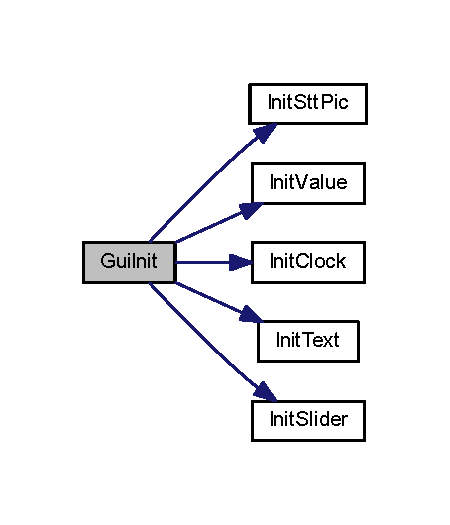
\includegraphics[width=216pt]{group___g_u_i_gafec26559ec22791fb442dd8f2a8f213e_cgraph}
\end{center}
\end{figure}




\-Here is the caller graph for this function\-:\nopagebreak
\begin{figure}[H]
\begin{center}
\leavevmode
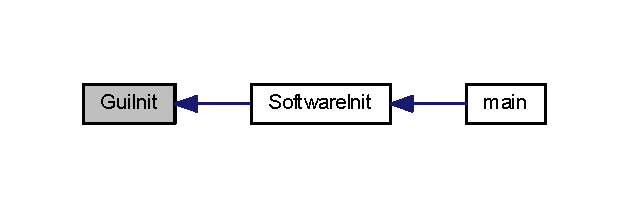
\includegraphics[width=302pt]{group___g_u_i_gafec26559ec22791fb442dd8f2a8f213e_icgraph}
\end{center}
\end{figure}


\hypertarget{group___g_u_i_ga60bf00524cdf8112890394a49a79f84c}{\index{\-G\-U\-I\-: A\-P\-P Group@{\-G\-U\-I\-: A\-P\-P Group}!\-Key\-Action@{\-Key\-Action}}
\index{\-Key\-Action@{\-Key\-Action}!GUI: APP Group@{\-G\-U\-I\-: A\-P\-P Group}}
\subsubsection[{\-Key\-Action}]{\setlength{\rightskip}{0pt plus 5cm}void {\bf \-Key\-Action} (
\begin{DoxyParamCaption}
\item[{{\bf \-S\-T\-R\-\_\-\-Gui} $\ast$}]{gui, }
\item[{{\bf \-S\-T\-R\-\_\-\-Key} $\ast$}]{key}
\end{DoxyParamCaption}
)}}\label{group___g_u_i_ga60bf00524cdf8112890394a49a79f84c}


人机交互界面按键响应 


\begin{DoxyParams}[1]{\-Parameters}
 & {\em 参数名} & 参数说明 \\
\hline
\mbox{\tt out}  & {\em gui} & \-G\-U\-I结构体指针 \\
\hline
\mbox{\tt in}  & {\em key} & 按键状态结构体指针 \\
\hline
\end{DoxyParams}

\begin{DoxyRetVals}{\-Return values}
{\em 无} & \\
\hline
\end{DoxyRetVals}
\begin{DoxyParagraph}{使用全局变量 }

\end{DoxyParagraph}
\begin{DoxyNote}{\-Note}
● 执行时间\-: \par
 ● 调用周期\-: 1ms \par
 ● 可否打断\-: 可以 \par

\end{DoxyNote}
\begin{DoxyParagraph}{注意\-:}
● 无 \par
 
\end{DoxyParagraph}

\hypertarget{group___m_a_n_a_g_e}{\section{\-Manage\-: \-A\-P\-P \-Group}
\label{group___m_a_n_a_g_e}\index{\-Manage\-: A\-P\-P Group@{\-Manage\-: A\-P\-P Group}}
}
\subsection*{\-Data \-Structures}
\begin{DoxyCompactItemize}
\item 
struct \hyperlink{struct_s_t_r___sys}{\-S\-T\-R\-\_\-\-Sys}
\begin{DoxyCompactList}\small\item\em 系统结构体 \end{DoxyCompactList}\end{DoxyCompactItemize}
\subsection*{\-Defines}
\begin{DoxyCompactItemize}
\item 
\hypertarget{group___m_a_n_a_g_e_gad13f8dea3a5243219cd2109520fdefe4}{\#define \hyperlink{group___m_a_n_a_g_e_gad13f8dea3a5243219cd2109520fdefe4}{\-S\-W\-\_\-\-V\-E\-R\-S\-I\-O\-N}~20}\label{group___m_a_n_a_g_e_gad13f8dea3a5243219cd2109520fdefe4}

\begin{DoxyCompactList}\small\item\em 软件版本 2.\-0 \end{DoxyCompactList}\item 
\hypertarget{group___m_a_n_a_g_e_ga8c5f6d47006c226d1cc5c20bac6ecf76}{\#define \hyperlink{group___m_a_n_a_g_e_ga8c5f6d47006c226d1cc5c20bac6ecf76}{\-S\-T\-R\-\_\-\-V\-E\-R\-S\-I\-O\-N}~\char`\"{}\-Smart\-L\-E\-D \-V2.\-0\char`\"{}}\label{group___m_a_n_a_g_e_ga8c5f6d47006c226d1cc5c20bac6ecf76}

\begin{DoxyCompactList}\small\item\em 软件版本 2.\-0 \end{DoxyCompactList}\end{DoxyCompactItemize}
\subsection*{\-Functions}
\begin{DoxyCompactItemize}
\item 
void \hyperlink{group___m_a_n_a_g_e_ga6ae21a567d8b7f88c319620bd458f1e2}{\-Sleep} (void)
\begin{DoxyCompactList}\small\item\em stm32进入睡眠状态函数 \end{DoxyCompactList}\item 
void \hyperlink{group___m_a_n_a_g_e_ga8dcf623cce7777facf0cc0223fab8e19}{\-Sys\-Stt\-Upd} (\hyperlink{struct_s_t_r___sys}{\-S\-T\-R\-\_\-\-Sys} $\ast$sys)
\begin{DoxyCompactList}\small\item\em 系统状态更新 \end{DoxyCompactList}\item 
\hypertarget{group___m_a_n_a_g_e_ga601c095b03e6638b39ed349f4c24b69e}{void \hyperlink{group___m_a_n_a_g_e_ga601c095b03e6638b39ed349f4c24b69e}{\-Software\-Init} (void)}\label{group___m_a_n_a_g_e_ga601c095b03e6638b39ed349f4c24b69e}

\begin{DoxyCompactList}\small\item\em 软件初始化函数 \end{DoxyCompactList}\item 
\hypertarget{group___m_a_n_a_g_e_gae5433f92dfcd0d1adfc3c045eab15253}{void \hyperlink{group___m_a_n_a_g_e_gae5433f92dfcd0d1adfc3c045eab15253}{\-Gui\-Data\-Upd} (\hyperlink{struct_s_t_r___sys}{\-S\-T\-R\-\_\-\-Sys} $\ast$sys)}\label{group___m_a_n_a_g_e_gae5433f92dfcd0d1adfc3c045eab15253}

\begin{DoxyCompactList}\small\item\em 更新人机界面数据 \end{DoxyCompactList}\item 
void \hyperlink{group___m_a_n_a_g_e_ga93f514700ccf00d08dbdcff7f1224eb2}{\-System\-Init} (void)
\begin{DoxyCompactList}\small\item\em 硬件初始化函数 \end{DoxyCompactList}\item 
void \hyperlink{group___m_a_n_a_g_e_gad7f568b58dcae6573d84519c01f70516}{\-Task} (void)
\begin{DoxyCompactList}\small\item\em 任务分派函数 \end{DoxyCompactList}\end{DoxyCompactItemize}
\subsection*{\-Variables}
\begin{DoxyCompactItemize}
\item 
\hypertarget{group___m_a_n_a_g_e_ga77104fa87f934b24a88a51ede198e668}{\hyperlink{struct_s_t_r___sys}{\-S\-T\-R\-\_\-\-Sys} \hyperlink{group___m_a_n_a_g_e_ga77104fa87f934b24a88a51ede198e668}{\-Sys}}\label{group___m_a_n_a_g_e_ga77104fa87f934b24a88a51ede198e668}

\begin{DoxyCompactList}\small\item\em 系统变量结构体 \end{DoxyCompactList}\item 
\hypertarget{group___m_a_n_a_g_e_ga77104fa87f934b24a88a51ede198e668}{\hyperlink{struct_s_t_r___sys}{\-S\-T\-R\-\_\-\-Sys} \hyperlink{group___m_a_n_a_g_e_ga77104fa87f934b24a88a51ede198e668}{\-Sys}}\label{group___m_a_n_a_g_e_ga77104fa87f934b24a88a51ede198e668}

\begin{DoxyCompactList}\small\item\em 系统变量结构体 \end{DoxyCompactList}\end{DoxyCompactItemize}


\subsection{\-Function \-Documentation}
\hypertarget{group___m_a_n_a_g_e_ga6ae21a567d8b7f88c319620bd458f1e2}{\index{\-Manage\-: A\-P\-P Group@{\-Manage\-: A\-P\-P Group}!\-Sleep@{\-Sleep}}
\index{\-Sleep@{\-Sleep}!Manage: APP Group@{\-Manage\-: A\-P\-P Group}}
\subsubsection[{\-Sleep}]{\setlength{\rightskip}{0pt plus 5cm}void {\bf \-Sleep} (
\begin{DoxyParamCaption}
\item[{void}]{}
\end{DoxyParamCaption}
)}}\label{group___m_a_n_a_g_e_ga6ae21a567d8b7f88c319620bd458f1e2}


stm32进入睡眠状态函数 


\begin{DoxyParams}{\-Parameters}
{\em 参数名} & 参数说明 \\
\hline
{\em 无} & \\
\hline
\end{DoxyParams}

\begin{DoxyRetVals}{\-Return values}
{\em 无} & \\
\hline
\end{DoxyRetVals}
\begin{DoxyParagraph}{使用全局变量 }

\end{DoxyParagraph}
\begin{DoxyNote}{\-Note}
● 执行时间\-: \par
 ● 调用周期\-: 触发调用 \par
 ● 可否打断\-: 可以 \par

\end{DoxyNote}
\begin{DoxyParagraph}{注意\-:}
● 无 \par
 
\end{DoxyParagraph}
\hypertarget{group___m_a_n_a_g_e_ga8dcf623cce7777facf0cc0223fab8e19}{\index{\-Manage\-: A\-P\-P Group@{\-Manage\-: A\-P\-P Group}!\-Sys\-Stt\-Upd@{\-Sys\-Stt\-Upd}}
\index{\-Sys\-Stt\-Upd@{\-Sys\-Stt\-Upd}!Manage: APP Group@{\-Manage\-: A\-P\-P Group}}
\subsubsection[{\-Sys\-Stt\-Upd}]{\setlength{\rightskip}{0pt plus 5cm}void {\bf \-Sys\-Stt\-Upd} (
\begin{DoxyParamCaption}
\item[{{\bf \-S\-T\-R\-\_\-\-Sys} $\ast$}]{sys}
\end{DoxyParamCaption}
)}}\label{group___m_a_n_a_g_e_ga8dcf623cce7777facf0cc0223fab8e19}


系统状态更新 

更新系统状态 \hypertarget{group___m_a_n_a_g_e_ga93f514700ccf00d08dbdcff7f1224eb2}{\index{\-Manage\-: A\-P\-P Group@{\-Manage\-: A\-P\-P Group}!\-System\-Init@{\-System\-Init}}
\index{\-System\-Init@{\-System\-Init}!Manage: APP Group@{\-Manage\-: A\-P\-P Group}}
\subsubsection[{\-System\-Init}]{\setlength{\rightskip}{0pt plus 5cm}void {\bf \-System\-Init} (
\begin{DoxyParamCaption}
\item[{void}]{}
\end{DoxyParamCaption}
)}}\label{group___m_a_n_a_g_e_ga93f514700ccf00d08dbdcff7f1224eb2}


硬件初始化函数 

硬件初始化函数


\begin{DoxyParams}{\-Parameters}
{\em 参数名} & 参数说明 \\
\hline
{\em 无} & \\
\hline
\end{DoxyParams}

\begin{DoxyRetVals}{\-Return values}
{\em 无} & \\
\hline
\end{DoxyRetVals}
\begin{DoxyParagraph}{使用全局变量 }

\end{DoxyParagraph}
\begin{DoxyNote}{\-Note}
● 执行时间\-: \par
 ● 调用周期\-: 触发调用, 初始化时调用 \par
 ● 可否打断\-: 可以 \par

\end{DoxyNote}
\begin{DoxyParagraph}{注意\-:}
● 无 \par
 
\end{DoxyParagraph}


\-Here is the call graph for this function\-:\nopagebreak
\begin{figure}[H]
\begin{center}
\leavevmode
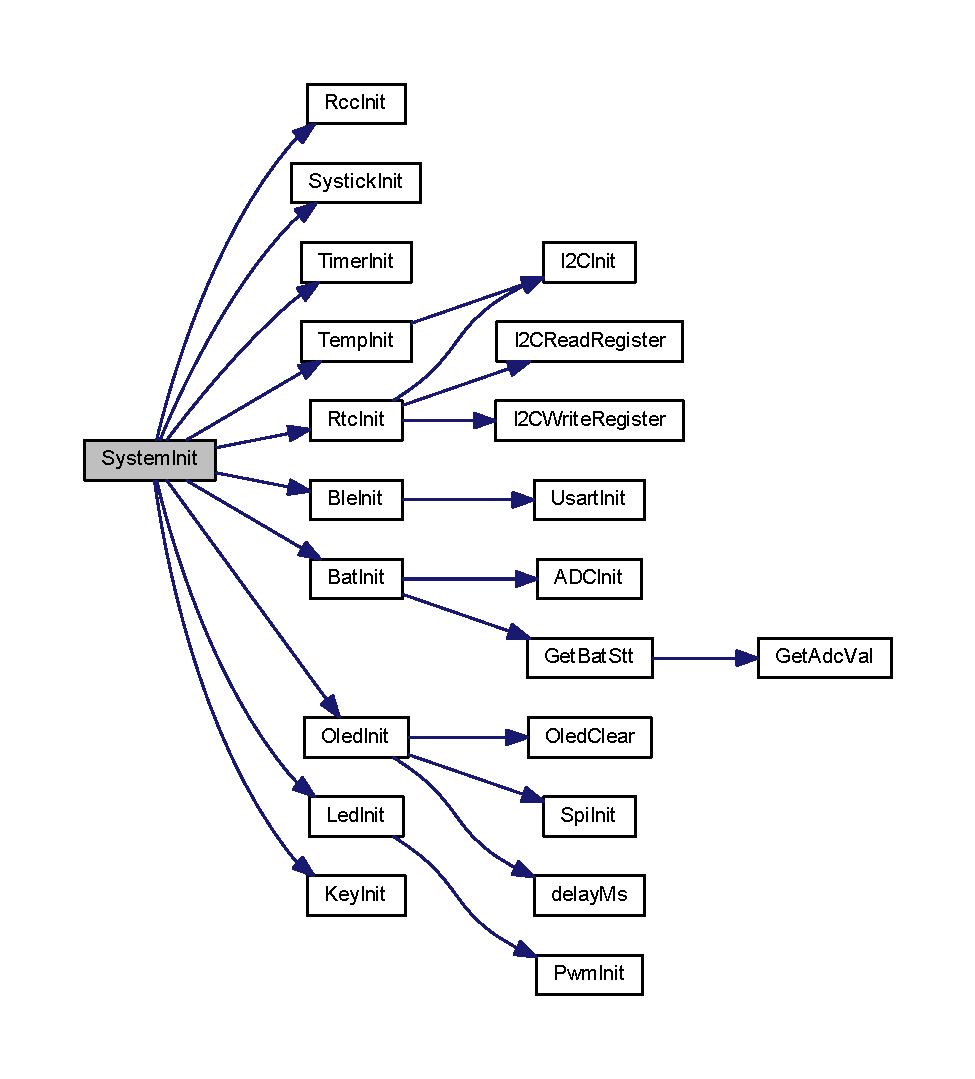
\includegraphics[width=350pt]{group___m_a_n_a_g_e_ga93f514700ccf00d08dbdcff7f1224eb2_cgraph}
\end{center}
\end{figure}




\-Here is the caller graph for this function\-:\nopagebreak
\begin{figure}[H]
\begin{center}
\leavevmode
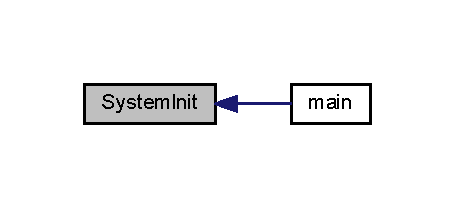
\includegraphics[width=218pt]{group___m_a_n_a_g_e_ga93f514700ccf00d08dbdcff7f1224eb2_icgraph}
\end{center}
\end{figure}


\hypertarget{group___m_a_n_a_g_e_gad7f568b58dcae6573d84519c01f70516}{\index{\-Manage\-: A\-P\-P Group@{\-Manage\-: A\-P\-P Group}!\-Task@{\-Task}}
\index{\-Task@{\-Task}!Manage: APP Group@{\-Manage\-: A\-P\-P Group}}
\subsubsection[{\-Task}]{\setlength{\rightskip}{0pt plus 5cm}void {\bf \-Task} (
\begin{DoxyParamCaption}
\item[{void}]{}
\end{DoxyParamCaption}
)}}\label{group___m_a_n_a_g_e_gad7f568b58dcae6573d84519c01f70516}


任务分派函数 


\begin{DoxyParams}{\-Parameters}
{\em 参数名} & 参数说明 \\
\hline
{\em 无} & \\
\hline
\end{DoxyParams}

\begin{DoxyRetVals}{\-Return values}
{\em 无} & \\
\hline
\end{DoxyRetVals}
\begin{DoxyNote}{\-Note}
● 调用周期\-: 500us调用\par
 $\ast$ 
\end{DoxyNote}
\begin{DoxyParagraph}{注意\-:}
● \par
 
\end{DoxyParagraph}


\-Here is the caller graph for this function\-:\nopagebreak
\begin{figure}[H]
\begin{center}
\leavevmode
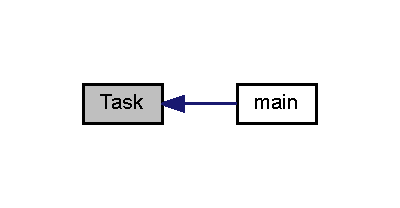
\includegraphics[width=192pt]{group___m_a_n_a_g_e_gad7f568b58dcae6573d84519c01f70516_icgraph}
\end{center}
\end{figure}



\hypertarget{group___m_a_i_n}{\section{main\-: \-A\-P\-P \-Group}
\label{group___m_a_i_n}\index{main\-: A\-P\-P Group@{main\-: A\-P\-P Group}}
}
\subsection*{\-Functions}
\begin{DoxyCompactItemize}
\item 
int \hyperlink{group___m_a_i_n_gae66f6b31b5ad750f1fe042a706a4e3d4}{main} ()
\begin{DoxyCompactList}\small\item\em main函数 \end{DoxyCompactList}\end{DoxyCompactItemize}


\subsection{\-Function \-Documentation}
\hypertarget{group___m_a_i_n_gae66f6b31b5ad750f1fe042a706a4e3d4}{\index{main\-: A\-P\-P Group@{main\-: A\-P\-P Group}!main@{main}}
\index{main@{main}!main: APP Group@{main\-: A\-P\-P Group}}
\subsubsection[{main}]{\setlength{\rightskip}{0pt plus 5cm}int {\bf main} (
\begin{DoxyParamCaption}
{}
\end{DoxyParamCaption}
)}}\label{group___m_a_i_n_gae66f6b31b5ad750f1fe042a706a4e3d4}


main函数 


\begin{DoxyParams}{\-Parameters}
{\em 参数名} & 参数说明 \\
\hline
{\em 无} & \\
\hline
\end{DoxyParams}

\begin{DoxyRetVals}{\-Return values}
{\em 无} & \\
\hline
\end{DoxyRetVals}
\begin{DoxyParagraph}{使用全局变量 }

\end{DoxyParagraph}
\begin{DoxyNote}{\-Note}
● 执行时间\-: \par
 ● 调用周期\-: \par
 ● 可否打断\-: 可以 \par

\end{DoxyNote}
\begin{DoxyParagraph}{注意\-:}
● 无 \par
 
\end{DoxyParagraph}


\-Here is the call graph for this function\-:\nopagebreak
\begin{figure}[H]
\begin{center}
\leavevmode
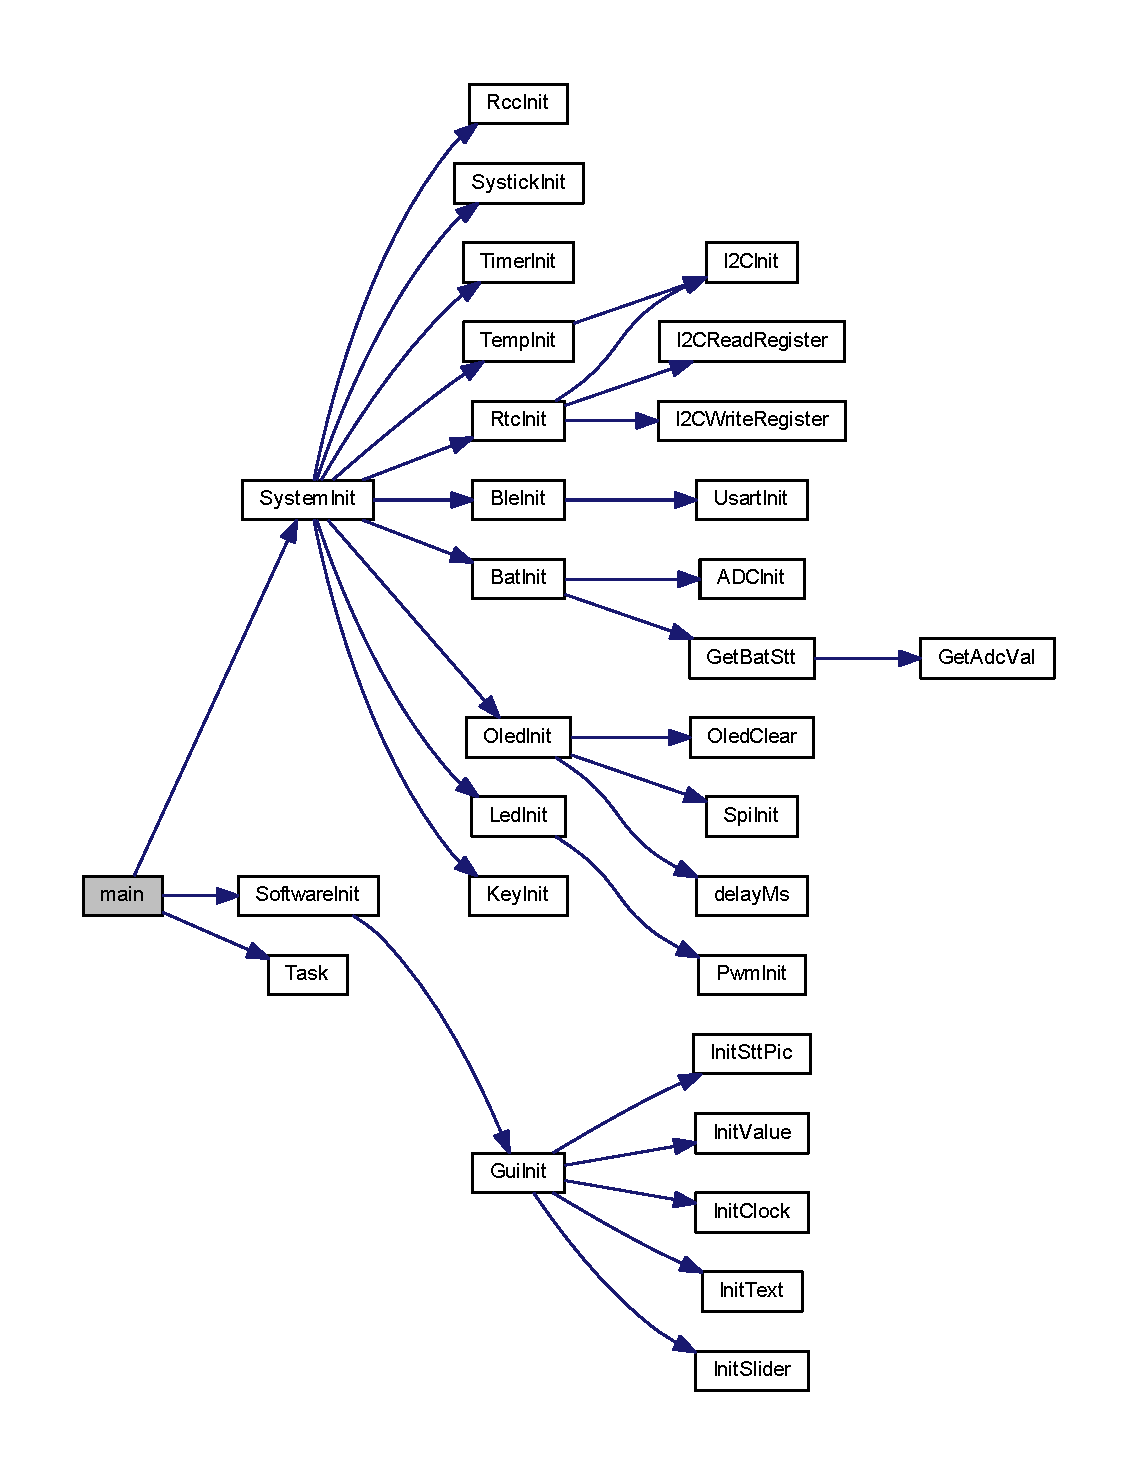
\includegraphics[width=350pt]{group___m_a_i_n_gae66f6b31b5ad750f1fe042a706a4e3d4_cgraph}
\end{center}
\end{figure}



\hypertarget{group___w_i_d_g_e_t}{\section{\-Widget\-: \-A\-P\-P \-Group}
\label{group___w_i_d_g_e_t}\index{\-Widget\-: A\-P\-P Group@{\-Widget\-: A\-P\-P Group}}
}
\subsection*{\-Data \-Structures}
\begin{DoxyCompactItemize}
\item 
struct \hyperlink{struct_s_t_r___slider}{\-S\-T\-R\-\_\-\-Slider}
\begin{DoxyCompactList}\small\item\em 滑动条结构体 \end{DoxyCompactList}\item 
struct \hyperlink{struct_s_t_r___text}{\-S\-T\-R\-\_\-\-Text}
\begin{DoxyCompactList}\small\item\em 静态文本结构体 \end{DoxyCompactList}\item 
struct \hyperlink{struct_s_t_r___stt_pic}{\-S\-T\-R\-\_\-\-Stt\-Pic}
\begin{DoxyCompactList}\small\item\em 状态图片组结构体 \end{DoxyCompactList}\item 
struct \hyperlink{struct_s_t_r___value}{\-S\-T\-R\-\_\-\-Value}
\begin{DoxyCompactList}\small\item\em 数值控件结构体 \end{DoxyCompactList}\item 
struct \hyperlink{struct_s_t_r___clock}{\-S\-T\-R\-\_\-\-Clock}
\begin{DoxyCompactList}\small\item\em 时钟控件结构体 \end{DoxyCompactList}\end{DoxyCompactItemize}
\subsection*{\-Enumerations}
\begin{DoxyCompactItemize}
\item 
enum \hyperlink{group___w_i_d_g_e_t_gad259d67a883a17bd30a95355be423d9f}{\-E\-N\-U\-M\-\_\-\-Clock\-Focus} \{ \*
{\bfseries \-F\-O\-C\-U\-S\-\_\-\-N\-O\-N\-E} =  0, 
{\bfseries \-F\-O\-C\-U\-S\-\_\-\-Y\-E\-A\-R} =  1, 
{\bfseries \-F\-O\-C\-U\-S\-\_\-\-M\-O\-N\-T\-H} =  2, 
{\bfseries \-F\-O\-C\-U\-S\-\_\-\-D\-A\-T\-E} =  3, 
\*
{\bfseries \-F\-O\-C\-U\-S\-\_\-\-H\-O\-U\-R} =  4, 
{\bfseries \-F\-O\-C\-U\-S\-\_\-\-M\-I\-N} =  5, 
{\bfseries \-F\-O\-C\-U\-S\-\_\-\-S\-E\-C} =  6
 \}
\begin{DoxyCompactList}\small\item\em 时钟选中状态枚举 \end{DoxyCompactList}\item 
enum \hyperlink{group___w_i_d_g_e_t_ga096d65323cbe1c9a55ddf6566972e0c7}{\-E\-N\-U\-M\-\_\-\-Clock\-Style} \{ \hyperlink{group___w_i_d_g_e_t_gga096d65323cbe1c9a55ddf6566972e0c7a2d2463feb28f4ce93e9dda0fcbab5203}{\-C\-L\-O\-C\-K\-\_\-\-B\-I\-G} =  0, 
\hyperlink{group___w_i_d_g_e_t_gga096d65323cbe1c9a55ddf6566972e0c7a8d2d7a3fb2433c570b55db4aa58288e1}{\-C\-L\-O\-C\-K\-\_\-\-S\-E\-T} =  1, 
\hyperlink{group___w_i_d_g_e_t_gga096d65323cbe1c9a55ddf6566972e0c7af2b0a3c4435e1f0c2a5cf42018332bc1}{\-C\-L\-O\-C\-K\-\_\-\-D\-A\-T} =  2, 
\hyperlink{group___w_i_d_g_e_t_gga096d65323cbe1c9a55ddf6566972e0c7a8b4cc99c547338a78acc1f4056d60c7e}{\-C\-L\-O\-C\-K\-\_\-\-F\-U\-L} =  3
 \}
\begin{DoxyCompactList}\small\item\em 时钟样式枚举 \end{DoxyCompactList}\end{DoxyCompactItemize}
\subsection*{\-Functions}
\begin{DoxyCompactItemize}
\item 
void \hyperlink{group___w_i_d_g_e_t_ga7338b1b845ab8569f825f48754d4702c}{\-Init\-Clock} (\hyperlink{group___b_s_p_gaed742c436da53c1080638ce6ef7d13de}{u8} x, \hyperlink{group___b_s_p_gaed742c436da53c1080638ce6ef7d13de}{u8} y, \hyperlink{group___b_s_p_gaed742c436da53c1080638ce6ef7d13de}{u8} style, \hyperlink{struct_s_t_r___time}{\-S\-T\-R\-\_\-\-Time} $\ast$time, \hyperlink{struct_s_t_r___clock}{\-S\-T\-R\-\_\-\-Clock} $\ast$clock)
\begin{DoxyCompactList}\small\item\em 初始化时钟控件 \end{DoxyCompactList}\item 
void \hyperlink{group___w_i_d_g_e_t_gae106cd7bf5dbfbc9806614193eb0f2b6}{\-Disp\-Clock} (\hyperlink{struct_s_t_r___clock}{\-S\-T\-R\-\_\-\-Clock} $\ast$clock, int x\-Offset)
\begin{DoxyCompactList}\small\item\em 显示时钟控件 \end{DoxyCompactList}\item 
void \hyperlink{group___w_i_d_g_e_t_ga5fa501fc4c260c0bd86b52471f33a411}{\-Init\-Stt\-Pic} (\hyperlink{group___b_s_p_gaed742c436da53c1080638ce6ef7d13de}{u8} x, \hyperlink{group___b_s_p_gaed742c436da53c1080638ce6ef7d13de}{u8} y, \hyperlink{group___b_s_p_gaed742c436da53c1080638ce6ef7d13de}{u8} width, \hyperlink{group___b_s_p_gaed742c436da53c1080638ce6ef7d13de}{u8} height, \hyperlink{group___b_s_p_gaed742c436da53c1080638ce6ef7d13de}{u8} $\ast$pic\-Base, \hyperlink{struct_s_t_r___stt_pic}{\-S\-T\-R\-\_\-\-Stt\-Pic} $\ast$stt\-Pic)
\begin{DoxyCompactList}\small\item\em 初始化图片组控件 \end{DoxyCompactList}\item 
void \hyperlink{group___w_i_d_g_e_t_gaa4a2492358bbb448b4bd8e1b9792bdb2}{\-Disp\-Stt\-Pic} (\hyperlink{struct_s_t_r___stt_pic}{\-S\-T\-R\-\_\-\-Stt\-Pic} $\ast$stt\-Pic, int x\-Offset)
\begin{DoxyCompactList}\small\item\em 图片组控件 \end{DoxyCompactList}\item 
void \hyperlink{group___w_i_d_g_e_t_ga7a6ad9f67f512cb71394be195152a1bc}{\-Init\-Value} (\hyperlink{group___b_s_p_gaed742c436da53c1080638ce6ef7d13de}{u8} x, \hyperlink{group___b_s_p_gaed742c436da53c1080638ce6ef7d13de}{u8} y, \hyperlink{group___b_s_p_gaed742c436da53c1080638ce6ef7d13de}{u8} dot, char $\ast$str, \hyperlink{struct_s_t_r___value}{\-S\-T\-R\-\_\-\-Value} $\ast$value)
\begin{DoxyCompactList}\small\item\em 初始化数值控件 \end{DoxyCompactList}\item 
void \hyperlink{group___w_i_d_g_e_t_gaf4e0de6239412535e03e36cd804c57b0}{\-Disp\-Value} (\hyperlink{struct_s_t_r___value}{\-S\-T\-R\-\_\-\-Value} $\ast$value, int x\-Offset)
\begin{DoxyCompactList}\small\item\em 数值显示控件 \end{DoxyCompactList}\item 
void \hyperlink{group___w_i_d_g_e_t_ga612551bd76b7c4640906e50cb9ee5f1e}{\-Init\-Slider} (\hyperlink{group___b_s_p_gaed742c436da53c1080638ce6ef7d13de}{u8} x, \hyperlink{group___b_s_p_gaed742c436da53c1080638ce6ef7d13de}{u8} y, \hyperlink{group___b_s_p_gaed742c436da53c1080638ce6ef7d13de}{u8} len, char $\ast$str, \hyperlink{struct_s_t_r___slider}{\-S\-T\-R\-\_\-\-Slider} $\ast$slider)
\begin{DoxyCompactList}\small\item\em 初始化进度条控件 \end{DoxyCompactList}\item 
void \hyperlink{group___w_i_d_g_e_t_ga6dce8af29d9d4e96029624f8d21af519}{\-Disp\-Slid} (\hyperlink{struct_s_t_r___slider}{\-S\-T\-R\-\_\-\-Slider} $\ast$slider, int x\-Offset)
\begin{DoxyCompactList}\small\item\em 进度条显示控件 \end{DoxyCompactList}\item 
void \hyperlink{group___w_i_d_g_e_t_gac18895bdc14f553f346c2b01e6fcc119}{\-Init\-Text} (\hyperlink{group___b_s_p_gaed742c436da53c1080638ce6ef7d13de}{u8} x, \hyperlink{group___b_s_p_gaed742c436da53c1080638ce6ef7d13de}{u8} y, char $\ast$str, \hyperlink{struct_s_t_r___text}{\-S\-T\-R\-\_\-\-Text} $\ast$text)
\begin{DoxyCompactList}\small\item\em 初始化静态文本控件 \end{DoxyCompactList}\item 
void \hyperlink{group___w_i_d_g_e_t_ga9684de3b62426e0d486fbdebe0e759ed}{\-Disp\-Text} (\hyperlink{struct_s_t_r___text}{\-S\-T\-R\-\_\-\-Text} $\ast$text, int x\-Offset)
\begin{DoxyCompactList}\small\item\em 静态文本显示控件 \end{DoxyCompactList}\end{DoxyCompactItemize}
\subsection*{\-Variables}
\begin{DoxyCompactItemize}
\item 
\hypertarget{group___w_i_d_g_e_t_gade592d4d7d3059dc93d2bb83b39b3db6}{const unsigned char \hyperlink{group___w_i_d_g_e_t_gade592d4d7d3059dc93d2bb83b39b3db6}{g\-Image\-\_\-\-L\-E\-D} \mbox{[}512\mbox{]}}\label{group___w_i_d_g_e_t_gade592d4d7d3059dc93d2bb83b39b3db6}

\begin{DoxyCompactList}\small\item\em \-L\-E\-D图标 \end{DoxyCompactList}\item 
\hypertarget{group___w_i_d_g_e_t_gaa649afc64d2f2a99b429fa4e5fb13d50}{const unsigned char \hyperlink{group___w_i_d_g_e_t_gaa649afc64d2f2a99b429fa4e5fb13d50}{g\-Image\-\_\-\-S\-E\-T\-T\-I\-N\-G} \mbox{[}512\mbox{]}}\label{group___w_i_d_g_e_t_gaa649afc64d2f2a99b429fa4e5fb13d50}

\begin{DoxyCompactList}\small\item\em 设置图标 \end{DoxyCompactList}\item 
\hypertarget{group___w_i_d_g_e_t_ga26e73b61ee22edf6ce4b9592a6d1ffd2}{const unsigned char \hyperlink{group___w_i_d_g_e_t_ga26e73b61ee22edf6ce4b9592a6d1ffd2}{g\-Image\-\_\-\-I\-N\-F\-O} \mbox{[}512\mbox{]}}\label{group___w_i_d_g_e_t_ga26e73b61ee22edf6ce4b9592a6d1ffd2}

\begin{DoxyCompactList}\small\item\em 信息图标 \end{DoxyCompactList}\item 
\hypertarget{group___w_i_d_g_e_t_ga42de702f802d2ab0de797d4712a516df}{const unsigned char \hyperlink{group___w_i_d_g_e_t_ga42de702f802d2ab0de797d4712a516df}{g\-Image\-\_\-\-L\-E\-D\-\_\-\-D\-I\-S\-A\-B\-L\-E} \mbox{[}512\mbox{]}}\label{group___w_i_d_g_e_t_ga42de702f802d2ab0de797d4712a516df}

\begin{DoxyCompactList}\small\item\em \-L\-E\-D禁止图标 \end{DoxyCompactList}\item 
\hypertarget{group___w_i_d_g_e_t_ga4e313eb11c9272ec38246bbc0f4cec42}{const unsigned char \hyperlink{group___w_i_d_g_e_t_ga4e313eb11c9272ec38246bbc0f4cec42}{font\-Time\-Num} \mbox{[}$\,$\mbox{]}\mbox{[}28\mbox{]}}\label{group___w_i_d_g_e_t_ga4e313eb11c9272ec38246bbc0f4cec42}

\begin{DoxyCompactList}\small\item\em 时间显示超大字体 \end{DoxyCompactList}\item 
const unsigned char \hyperlink{group___w_i_d_g_e_t_ga934cfdf8aedca0ff9a8794005da8d5e0}{font\-Time\-Colon} \mbox{[}$\,$\mbox{]}\mbox{[}16\mbox{]}
\begin{DoxyCompactList}\small\item\em 时间显示用的冒号 \end{DoxyCompactList}\item 
const unsigned char \hyperlink{group___w_i_d_g_e_t_ga9cac21b10aac988fd92e2cd2c78a4319}{font\-Battery} \mbox{[}$\,$\mbox{]}\mbox{[}10\mbox{]}
\begin{DoxyCompactList}\small\item\em 电量显示图标 \end{DoxyCompactList}\item 
const unsigned char \hyperlink{group___w_i_d_g_e_t_gae789ac73b9f8bf563ff477571af3e532}{font\-B\-L\-E} \mbox{[}$\,$\mbox{]}\mbox{[}10\mbox{]}
\begin{DoxyCompactList}\small\item\em 蓝牙图标 \end{DoxyCompactList}\item 
const unsigned char \hyperlink{group___w_i_d_g_e_t_ga4281d2c990312a449f8115a73da5d4b6}{font\-Delay} \mbox{[}$\,$\mbox{]}\mbox{[}15\mbox{]}
\begin{DoxyCompactList}\small\item\em 时钟图标 \end{DoxyCompactList}\item 
const unsigned char \hyperlink{group___w_i_d_g_e_t_ga7ef23e7312ba1eef34a75bae365cf3e3}{font\-Enable} \mbox{[}$\,$\mbox{]}\mbox{[}8\mbox{]}
\begin{DoxyCompactList}\small\item\em 勾选框图标 \end{DoxyCompactList}\item 
const unsigned char \hyperlink{group___w_i_d_g_e_t_ga934307f74cc38f1062d272ab796d7715}{font\-Slide} \mbox{[}$\,$\mbox{]}\mbox{[}100\mbox{]}
\begin{DoxyCompactList}\small\item\em 进度条图标 \end{DoxyCompactList}\item 
\hypertarget{group___w_i_d_g_e_t_ga4e313eb11c9272ec38246bbc0f4cec42}{const unsigned char \hyperlink{group___w_i_d_g_e_t_ga4e313eb11c9272ec38246bbc0f4cec42}{font\-Time\-Num} \mbox{[}$\,$\mbox{]}\mbox{[}28\mbox{]}}\label{group___w_i_d_g_e_t_ga4e313eb11c9272ec38246bbc0f4cec42}

\begin{DoxyCompactList}\small\item\em 时间显示超大字体 \end{DoxyCompactList}\item 
\hypertarget{group___w_i_d_g_e_t_ga9cac21b10aac988fd92e2cd2c78a4319}{const unsigned char \hyperlink{group___w_i_d_g_e_t_ga9cac21b10aac988fd92e2cd2c78a4319}{font\-Battery} \mbox{[}$\,$\mbox{]}\mbox{[}10\mbox{]}}\label{group___w_i_d_g_e_t_ga9cac21b10aac988fd92e2cd2c78a4319}

\begin{DoxyCompactList}\small\item\em 电量显示图标 \end{DoxyCompactList}\item 
\hypertarget{group___w_i_d_g_e_t_gae789ac73b9f8bf563ff477571af3e532}{const unsigned char \hyperlink{group___w_i_d_g_e_t_gae789ac73b9f8bf563ff477571af3e532}{font\-B\-L\-E} \mbox{[}$\,$\mbox{]}\mbox{[}10\mbox{]}}\label{group___w_i_d_g_e_t_gae789ac73b9f8bf563ff477571af3e532}

\begin{DoxyCompactList}\small\item\em 蓝牙图标 \end{DoxyCompactList}\item 
\hypertarget{group___w_i_d_g_e_t_ga934cfdf8aedca0ff9a8794005da8d5e0}{const unsigned char \hyperlink{group___w_i_d_g_e_t_ga934cfdf8aedca0ff9a8794005da8d5e0}{font\-Time\-Colon} \mbox{[}$\,$\mbox{]}\mbox{[}16\mbox{]}}\label{group___w_i_d_g_e_t_ga934cfdf8aedca0ff9a8794005da8d5e0}

\begin{DoxyCompactList}\small\item\em 时间显示用的冒号 \end{DoxyCompactList}\item 
\hypertarget{group___w_i_d_g_e_t_ga7ef23e7312ba1eef34a75bae365cf3e3}{const unsigned char \hyperlink{group___w_i_d_g_e_t_ga7ef23e7312ba1eef34a75bae365cf3e3}{font\-Enable} \mbox{[}$\,$\mbox{]}\mbox{[}8\mbox{]}}\label{group___w_i_d_g_e_t_ga7ef23e7312ba1eef34a75bae365cf3e3}

\begin{DoxyCompactList}\small\item\em 勾选框图标 \end{DoxyCompactList}\item 
\hypertarget{group___w_i_d_g_e_t_ga4281d2c990312a449f8115a73da5d4b6}{const unsigned char \hyperlink{group___w_i_d_g_e_t_ga4281d2c990312a449f8115a73da5d4b6}{font\-Delay} \mbox{[}$\,$\mbox{]}\mbox{[}15\mbox{]}}\label{group___w_i_d_g_e_t_ga4281d2c990312a449f8115a73da5d4b6}

\begin{DoxyCompactList}\small\item\em 时钟图标 \end{DoxyCompactList}\item 
\hypertarget{group___w_i_d_g_e_t_gaf4bc560cf5a8012c545d0dd42ad1c8db}{const unsigned char \hyperlink{group___w_i_d_g_e_t_gaf4bc560cf5a8012c545d0dd42ad1c8db}{font\-Slide} \mbox{[}100\mbox{]}}\label{group___w_i_d_g_e_t_gaf4bc560cf5a8012c545d0dd42ad1c8db}

\begin{DoxyCompactList}\small\item\em 进度条图标 \end{DoxyCompactList}\end{DoxyCompactItemize}


\subsection{\-Enumeration \-Type \-Documentation}
\hypertarget{group___w_i_d_g_e_t_ga096d65323cbe1c9a55ddf6566972e0c7}{\index{\-Widget\-: A\-P\-P Group@{\-Widget\-: A\-P\-P Group}!\-E\-N\-U\-M\-\_\-\-Clock\-Style@{\-E\-N\-U\-M\-\_\-\-Clock\-Style}}
\index{\-E\-N\-U\-M\-\_\-\-Clock\-Style@{\-E\-N\-U\-M\-\_\-\-Clock\-Style}!Widget: APP Group@{\-Widget\-: A\-P\-P Group}}
\subsubsection[{\-E\-N\-U\-M\-\_\-\-Clock\-Style}]{\setlength{\rightskip}{0pt plus 5cm}enum {\bf \-E\-N\-U\-M\-\_\-\-Clock\-Style}}}\label{group___w_i_d_g_e_t_ga096d65323cbe1c9a55ddf6566972e0c7}


时钟样式枚举 

\begin{Desc}
\item[\-Enumerator\-: ]\par
\begin{description}
\index{\-C\-L\-O\-C\-K\-\_\-\-B\-I\-G@{\-C\-L\-O\-C\-K\-\_\-\-B\-I\-G}!\-Widget\-: A\-P\-P Group@{\-Widget\-: A\-P\-P Group}}\index{\-Widget\-: A\-P\-P Group@{\-Widget\-: A\-P\-P Group}!\-C\-L\-O\-C\-K\-\_\-\-B\-I\-G@{\-C\-L\-O\-C\-K\-\_\-\-B\-I\-G}}\item[{\em 
\hypertarget{group___w_i_d_g_e_t_gga096d65323cbe1c9a55ddf6566972e0c7a2d2463feb28f4ce93e9dda0fcbab5203}{\-C\-L\-O\-C\-K\-\_\-\-B\-I\-G}\label{group___w_i_d_g_e_t_gga096d65323cbe1c9a55ddf6566972e0c7a2d2463feb28f4ce93e9dda0fcbab5203}
}]首页大时钟样式 \index{\-C\-L\-O\-C\-K\-\_\-\-S\-E\-T@{\-C\-L\-O\-C\-K\-\_\-\-S\-E\-T}!\-Widget\-: A\-P\-P Group@{\-Widget\-: A\-P\-P Group}}\index{\-Widget\-: A\-P\-P Group@{\-Widget\-: A\-P\-P Group}!\-C\-L\-O\-C\-K\-\_\-\-S\-E\-T@{\-C\-L\-O\-C\-K\-\_\-\-S\-E\-T}}\item[{\em 
\hypertarget{group___w_i_d_g_e_t_gga096d65323cbe1c9a55ddf6566972e0c7a8d2d7a3fb2433c570b55db4aa58288e1}{\-C\-L\-O\-C\-K\-\_\-\-S\-E\-T}\label{group___w_i_d_g_e_t_gga096d65323cbe1c9a55ddf6566972e0c7a8d2d7a3fb2433c570b55db4aa58288e1}
}]日期时间设置样式 \index{\-C\-L\-O\-C\-K\-\_\-\-D\-A\-T@{\-C\-L\-O\-C\-K\-\_\-\-D\-A\-T}!\-Widget\-: A\-P\-P Group@{\-Widget\-: A\-P\-P Group}}\index{\-Widget\-: A\-P\-P Group@{\-Widget\-: A\-P\-P Group}!\-C\-L\-O\-C\-K\-\_\-\-D\-A\-T@{\-C\-L\-O\-C\-K\-\_\-\-D\-A\-T}}\item[{\em 
\hypertarget{group___w_i_d_g_e_t_gga096d65323cbe1c9a55ddf6566972e0c7af2b0a3c4435e1f0c2a5cf42018332bc1}{\-C\-L\-O\-C\-K\-\_\-\-D\-A\-T}\label{group___w_i_d_g_e_t_gga096d65323cbe1c9a55ddf6566972e0c7af2b0a3c4435e1f0c2a5cf42018332bc1}
}]仅显示日期样式 \index{\-C\-L\-O\-C\-K\-\_\-\-F\-U\-L@{\-C\-L\-O\-C\-K\-\_\-\-F\-U\-L}!\-Widget\-: A\-P\-P Group@{\-Widget\-: A\-P\-P Group}}\index{\-Widget\-: A\-P\-P Group@{\-Widget\-: A\-P\-P Group}!\-C\-L\-O\-C\-K\-\_\-\-F\-U\-L@{\-C\-L\-O\-C\-K\-\_\-\-F\-U\-L}}\item[{\em 
\hypertarget{group___w_i_d_g_e_t_gga096d65323cbe1c9a55ddf6566972e0c7a8b4cc99c547338a78acc1f4056d60c7e}{\-C\-L\-O\-C\-K\-\_\-\-F\-U\-L}\label{group___w_i_d_g_e_t_gga096d65323cbe1c9a55ddf6566972e0c7a8b4cc99c547338a78acc1f4056d60c7e}
}]完整显示样式 \end{description}
\end{Desc}



\subsection{\-Function \-Documentation}
\hypertarget{group___w_i_d_g_e_t_gae106cd7bf5dbfbc9806614193eb0f2b6}{\index{\-Widget\-: A\-P\-P Group@{\-Widget\-: A\-P\-P Group}!\-Disp\-Clock@{\-Disp\-Clock}}
\index{\-Disp\-Clock@{\-Disp\-Clock}!Widget: APP Group@{\-Widget\-: A\-P\-P Group}}
\subsubsection[{\-Disp\-Clock}]{\setlength{\rightskip}{0pt plus 5cm}void {\bf \-Disp\-Clock} (
\begin{DoxyParamCaption}
\item[{{\bf \-S\-T\-R\-\_\-\-Clock} $\ast$}]{clock, }
\item[{int}]{x\-Offset}
\end{DoxyParamCaption}
)}}\label{group___w_i_d_g_e_t_gae106cd7bf5dbfbc9806614193eb0f2b6}


显示时钟控件 


\begin{DoxyParams}[1]{\-Parameters}
 & {\em 参数名} & 参数说明 \\
\hline
\mbox{\tt in}  & {\em clock} & 时钟控件指针 \\
\hline
\mbox{\tt in}  & {\em x\-Offset} & x轴偏移, 页面滑入滑出时用 \\
\hline
\end{DoxyParams}

\begin{DoxyRetVals}{\-Return values}
{\em 无} & \\
\hline
\end{DoxyRetVals}
\begin{DoxyParagraph}{使用全局变量 }

\end{DoxyParagraph}
\begin{DoxyNote}{\-Note}
● 执行时间\-: \par
 ● 调用周期\-: 触发调用 \par
 ● 可否打断\-: 可以 \par

\end{DoxyNote}
\begin{DoxyParagraph}{注意\-:}
● 无 \par
 
\end{DoxyParagraph}
\hypertarget{group___w_i_d_g_e_t_ga6dce8af29d9d4e96029624f8d21af519}{\index{\-Widget\-: A\-P\-P Group@{\-Widget\-: A\-P\-P Group}!\-Disp\-Slid@{\-Disp\-Slid}}
\index{\-Disp\-Slid@{\-Disp\-Slid}!Widget: APP Group@{\-Widget\-: A\-P\-P Group}}
\subsubsection[{\-Disp\-Slid}]{\setlength{\rightskip}{0pt plus 5cm}void {\bf \-Disp\-Slid} (
\begin{DoxyParamCaption}
\item[{{\bf \-S\-T\-R\-\_\-\-Slider} $\ast$}]{slider, }
\item[{int}]{x\-Offset}
\end{DoxyParamCaption}
)}}\label{group___w_i_d_g_e_t_ga6dce8af29d9d4e96029624f8d21af519}


进度条显示控件 


\begin{DoxyParams}[1]{\-Parameters}
 & {\em 参数名} & 参数说明 \\
\hline
\mbox{\tt in}  & {\em slider} & 进度条控件指针 \\
\hline
\mbox{\tt in}  & {\em x\-Offset} & x轴偏移, 页面滑入滑出时用 \\
\hline
\end{DoxyParams}

\begin{DoxyRetVals}{\-Return values}
{\em 无} & \\
\hline
\end{DoxyRetVals}
\begin{DoxyParagraph}{使用全局变量 }

\end{DoxyParagraph}
\begin{DoxyNote}{\-Note}
● 执行时间\-: \par
 ● 调用周期\-: 触发调用 \par
 ● 可否打断\-: 可以 \par

\end{DoxyNote}
\begin{DoxyParagraph}{注意\-:}
● 无 \par
 
\end{DoxyParagraph}


\-Here is the call graph for this function\-:\nopagebreak
\begin{figure}[H]
\begin{center}
\leavevmode
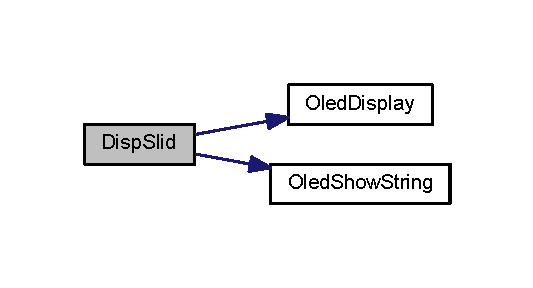
\includegraphics[width=256pt]{group___w_i_d_g_e_t_ga6dce8af29d9d4e96029624f8d21af519_cgraph}
\end{center}
\end{figure}


\hypertarget{group___w_i_d_g_e_t_gaa4a2492358bbb448b4bd8e1b9792bdb2}{\index{\-Widget\-: A\-P\-P Group@{\-Widget\-: A\-P\-P Group}!\-Disp\-Stt\-Pic@{\-Disp\-Stt\-Pic}}
\index{\-Disp\-Stt\-Pic@{\-Disp\-Stt\-Pic}!Widget: APP Group@{\-Widget\-: A\-P\-P Group}}
\subsubsection[{\-Disp\-Stt\-Pic}]{\setlength{\rightskip}{0pt plus 5cm}void {\bf \-Disp\-Stt\-Pic} (
\begin{DoxyParamCaption}
\item[{{\bf \-S\-T\-R\-\_\-\-Stt\-Pic} $\ast$}]{stt\-Pic, }
\item[{int}]{x\-Offset}
\end{DoxyParamCaption}
)}}\label{group___w_i_d_g_e_t_gaa4a2492358bbb448b4bd8e1b9792bdb2}


图片组控件 

显示图片组控件


\begin{DoxyParams}[1]{\-Parameters}
 & {\em 参数名} & 参数说明 \\
\hline
\mbox{\tt in}  & {\em stt\-Pic} & 控件指针 \\
\hline
\mbox{\tt in}  & {\em x\-Offset} & x轴偏移, 页面滑入滑出时用 \\
\hline
\end{DoxyParams}

\begin{DoxyRetVals}{\-Return values}
{\em 无} & \\
\hline
\end{DoxyRetVals}
\begin{DoxyParagraph}{使用全局变量 }

\end{DoxyParagraph}
\begin{DoxyNote}{\-Note}
● 执行时间\-: \par
 ● 调用周期\-: 触发调用 \par
 ● 可否打断\-: 可以 \par

\end{DoxyNote}
\begin{DoxyParagraph}{注意\-:}
● 该控件是指某个系统状态,不同的状态对应显示不同的图片,如电池电量、蓝牙状态、延时关灯状态等 \par
 
\end{DoxyParagraph}


\-Here is the call graph for this function\-:\nopagebreak
\begin{figure}[H]
\begin{center}
\leavevmode
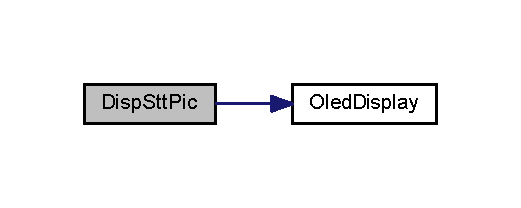
\includegraphics[width=250pt]{group___w_i_d_g_e_t_gaa4a2492358bbb448b4bd8e1b9792bdb2_cgraph}
\end{center}
\end{figure}


\hypertarget{group___w_i_d_g_e_t_ga9684de3b62426e0d486fbdebe0e759ed}{\index{\-Widget\-: A\-P\-P Group@{\-Widget\-: A\-P\-P Group}!\-Disp\-Text@{\-Disp\-Text}}
\index{\-Disp\-Text@{\-Disp\-Text}!Widget: APP Group@{\-Widget\-: A\-P\-P Group}}
\subsubsection[{\-Disp\-Text}]{\setlength{\rightskip}{0pt plus 5cm}void {\bf \-Disp\-Text} (
\begin{DoxyParamCaption}
\item[{{\bf \-S\-T\-R\-\_\-\-Text} $\ast$}]{text, }
\item[{int}]{x\-Offset}
\end{DoxyParamCaption}
)}}\label{group___w_i_d_g_e_t_ga9684de3b62426e0d486fbdebe0e759ed}


静态文本显示控件 


\begin{DoxyParams}[1]{\-Parameters}
 & {\em 参数名} & 参数说明 \\
\hline
\mbox{\tt in}  & {\em text} & 静态文本控件指针 \\
\hline
\mbox{\tt in}  & {\em x\-Offset} & x轴偏移, 页面滑入滑出时用 \\
\hline
\end{DoxyParams}

\begin{DoxyRetVals}{\-Return values}
{\em 无} & \\
\hline
\end{DoxyRetVals}
\begin{DoxyParagraph}{使用全局变量 }

\end{DoxyParagraph}
\begin{DoxyNote}{\-Note}
● 执行时间\-: \par
 ● 调用周期\-: 触发调用 \par
 ● 可否打断\-: 可以 \par

\end{DoxyNote}
\begin{DoxyParagraph}{注意\-:}
● 无 \par
 
\end{DoxyParagraph}


\-Here is the call graph for this function\-:\nopagebreak
\begin{figure}[H]
\begin{center}
\leavevmode
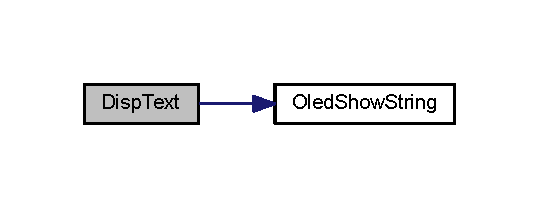
\includegraphics[width=258pt]{group___w_i_d_g_e_t_ga9684de3b62426e0d486fbdebe0e759ed_cgraph}
\end{center}
\end{figure}


\hypertarget{group___w_i_d_g_e_t_gaf4e0de6239412535e03e36cd804c57b0}{\index{\-Widget\-: A\-P\-P Group@{\-Widget\-: A\-P\-P Group}!\-Disp\-Value@{\-Disp\-Value}}
\index{\-Disp\-Value@{\-Disp\-Value}!Widget: APP Group@{\-Widget\-: A\-P\-P Group}}
\subsubsection[{\-Disp\-Value}]{\setlength{\rightskip}{0pt plus 5cm}void {\bf \-Disp\-Value} (
\begin{DoxyParamCaption}
\item[{{\bf \-S\-T\-R\-\_\-\-Value} $\ast$}]{value, }
\item[{int}]{x\-Offset}
\end{DoxyParamCaption}
)}}\label{group___w_i_d_g_e_t_gaf4e0de6239412535e03e36cd804c57b0}


数值显示控件 

显示数值控件


\begin{DoxyParams}[1]{\-Parameters}
 & {\em 参数名} & 参数说明 \\
\hline
\mbox{\tt in}  & {\em value} & 数值控件指针 \\
\hline
\mbox{\tt in}  & {\em x\-Offset} & x轴偏移, 页面滑入滑出时用 \\
\hline
\end{DoxyParams}

\begin{DoxyRetVals}{\-Return values}
{\em 无} & \\
\hline
\end{DoxyRetVals}
\begin{DoxyParagraph}{使用全局变量 }

\end{DoxyParagraph}
\begin{DoxyNote}{\-Note}
● 执行时间\-: \par
 ● 调用周期\-: 触发调用 \par
 ● 可否打断\-: 可以 \par

\end{DoxyNote}
\begin{DoxyParagraph}{注意\-:}
● 无 \par
 
\end{DoxyParagraph}


\-Here is the call graph for this function\-:\nopagebreak
\begin{figure}[H]
\begin{center}
\leavevmode
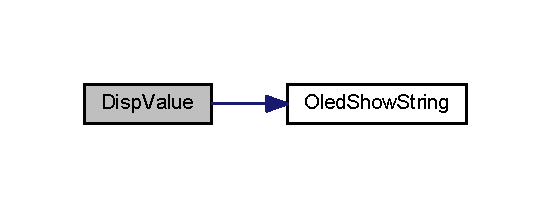
\includegraphics[width=264pt]{group___w_i_d_g_e_t_gaf4e0de6239412535e03e36cd804c57b0_cgraph}
\end{center}
\end{figure}


\hypertarget{group___w_i_d_g_e_t_ga7338b1b845ab8569f825f48754d4702c}{\index{\-Widget\-: A\-P\-P Group@{\-Widget\-: A\-P\-P Group}!\-Init\-Clock@{\-Init\-Clock}}
\index{\-Init\-Clock@{\-Init\-Clock}!Widget: APP Group@{\-Widget\-: A\-P\-P Group}}
\subsubsection[{\-Init\-Clock}]{\setlength{\rightskip}{0pt plus 5cm}void {\bf \-Init\-Clock} (
\begin{DoxyParamCaption}
\item[{{\bf u8}}]{x, }
\item[{{\bf u8}}]{y, }
\item[{{\bf u8}}]{style, }
\item[{{\bf \-S\-T\-R\-\_\-\-Time} $\ast$}]{time, }
\item[{{\bf \-S\-T\-R\-\_\-\-Clock} $\ast$}]{clock}
\end{DoxyParamCaption}
)}}\label{group___w_i_d_g_e_t_ga7338b1b845ab8569f825f48754d4702c}


初始化时钟控件 


\begin{DoxyParams}[1]{\-Parameters}
 & {\em 参数名} & 参数说明 \\
\hline
\mbox{\tt in}  & {\em x} & x轴坐标 \\
\hline
\mbox{\tt in}  & {\em y} & y轴坐标 \\
\hline
\mbox{\tt in}  & {\em style} & 显示样式 \\
\hline
\mbox{\tt in}  & {\em time} & 时间结构体指针 \\
\hline
\mbox{\tt out}  & {\em clock} & 时钟控件指针 \\
\hline
\end{DoxyParams}

\begin{DoxyRetVals}{\-Return values}
{\em 无} & \\
\hline
\end{DoxyRetVals}
\begin{DoxyParagraph}{使用全局变量 }

\end{DoxyParagraph}
\begin{DoxyNote}{\-Note}
● 执行时间\-: \par
 ● 调用周期\-: 触发调用, 初始化时调用 \par
 ● 可否打断\-: 可以 \par

\end{DoxyNote}
\begin{DoxyParagraph}{注意\-:}
● 无 \par
 
\end{DoxyParagraph}


\-Here is the caller graph for this function\-:\nopagebreak
\begin{figure}[H]
\begin{center}
\leavevmode
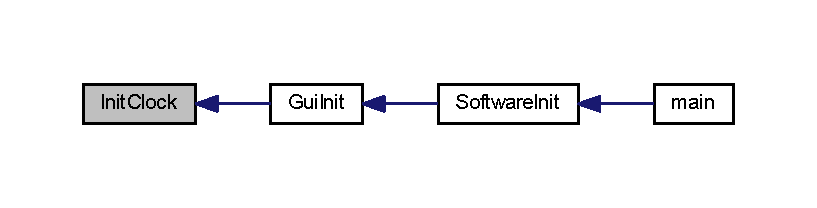
\includegraphics[width=350pt]{group___w_i_d_g_e_t_ga7338b1b845ab8569f825f48754d4702c_icgraph}
\end{center}
\end{figure}


\hypertarget{group___w_i_d_g_e_t_ga612551bd76b7c4640906e50cb9ee5f1e}{\index{\-Widget\-: A\-P\-P Group@{\-Widget\-: A\-P\-P Group}!\-Init\-Slider@{\-Init\-Slider}}
\index{\-Init\-Slider@{\-Init\-Slider}!Widget: APP Group@{\-Widget\-: A\-P\-P Group}}
\subsubsection[{\-Init\-Slider}]{\setlength{\rightskip}{0pt plus 5cm}void {\bf \-Init\-Slider} (
\begin{DoxyParamCaption}
\item[{{\bf u8}}]{x, }
\item[{{\bf u8}}]{y, }
\item[{{\bf u8}}]{len, }
\item[{char $\ast$}]{str, }
\item[{{\bf \-S\-T\-R\-\_\-\-Slider} $\ast$}]{slider}
\end{DoxyParamCaption}
)}}\label{group___w_i_d_g_e_t_ga612551bd76b7c4640906e50cb9ee5f1e}


初始化进度条控件 


\begin{DoxyParams}[1]{\-Parameters}
 & {\em 参数名} & 参数说明 \\
\hline
\mbox{\tt in}  & {\em x} & x轴坐标 \\
\hline
\mbox{\tt in}  & {\em y} & y轴坐标 \\
\hline
\mbox{\tt in}  & {\em len} & 进度条长度 \\
\hline
\mbox{\tt in}  & {\em str} & 单位字符串 \\
\hline
\mbox{\tt out}  & {\em slider} & 进度条控件指针 \\
\hline
\end{DoxyParams}

\begin{DoxyRetVals}{\-Return values}
{\em 无} & \\
\hline
\end{DoxyRetVals}
\begin{DoxyParagraph}{使用全局变量 }

\end{DoxyParagraph}
\begin{DoxyNote}{\-Note}
● 执行时间\-: \par
 ● 调用周期\-: 触发调用, 初始化时调用 \par
 ● 可否打断\-: 可以 \par

\end{DoxyNote}
\begin{DoxyParagraph}{注意\-:}
● 无 \par
 
\end{DoxyParagraph}


\-Here is the caller graph for this function\-:\nopagebreak
\begin{figure}[H]
\begin{center}
\leavevmode
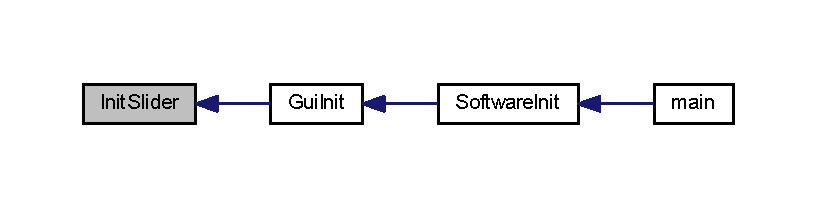
\includegraphics[width=350pt]{group___w_i_d_g_e_t_ga612551bd76b7c4640906e50cb9ee5f1e_icgraph}
\end{center}
\end{figure}


\hypertarget{group___w_i_d_g_e_t_ga5fa501fc4c260c0bd86b52471f33a411}{\index{\-Widget\-: A\-P\-P Group@{\-Widget\-: A\-P\-P Group}!\-Init\-Stt\-Pic@{\-Init\-Stt\-Pic}}
\index{\-Init\-Stt\-Pic@{\-Init\-Stt\-Pic}!Widget: APP Group@{\-Widget\-: A\-P\-P Group}}
\subsubsection[{\-Init\-Stt\-Pic}]{\setlength{\rightskip}{0pt plus 5cm}void {\bf \-Init\-Stt\-Pic} (
\begin{DoxyParamCaption}
\item[{{\bf u8}}]{x, }
\item[{{\bf u8}}]{y, }
\item[{{\bf u8}}]{width, }
\item[{{\bf u8}}]{height, }
\item[{{\bf u8} $\ast$}]{pic\-Base, }
\item[{{\bf \-S\-T\-R\-\_\-\-Stt\-Pic} $\ast$}]{stt\-Pic}
\end{DoxyParamCaption}
)}}\label{group___w_i_d_g_e_t_ga5fa501fc4c260c0bd86b52471f33a411}


初始化图片组控件 


\begin{DoxyParams}[1]{\-Parameters}
 & {\em 参数名} & 参数说明 \\
\hline
\mbox{\tt in}  & {\em x} & x轴坐标 \\
\hline
\mbox{\tt in}  & {\em y} & y轴坐标 \\
\hline
\mbox{\tt in}  & {\em width} & 宽 \\
\hline
\mbox{\tt in}  & {\em height} & 高 \\
\hline
\mbox{\tt in}  & {\em pic\-Base} & 图片指针 \\
\hline
\mbox{\tt out}  & {\em stt\-Pic} & 图片组控件指针 \\
\hline
\end{DoxyParams}

\begin{DoxyRetVals}{\-Return values}
{\em 无} & \\
\hline
\end{DoxyRetVals}
\begin{DoxyParagraph}{使用全局变量 }

\end{DoxyParagraph}
\begin{DoxyNote}{\-Note}
● 执行时间\-: \par
 ● 调用周期\-: 触发调用, 初始化时调用 \par
 ● 可否打断\-: 可以 \par

\end{DoxyNote}
\begin{DoxyParagraph}{注意\-:}
● 无 \par
 
\end{DoxyParagraph}


\-Here is the caller graph for this function\-:\nopagebreak
\begin{figure}[H]
\begin{center}
\leavevmode
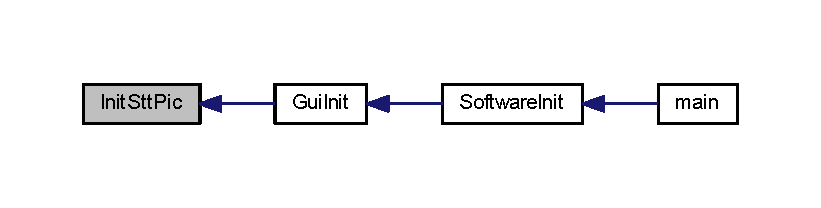
\includegraphics[width=350pt]{group___w_i_d_g_e_t_ga5fa501fc4c260c0bd86b52471f33a411_icgraph}
\end{center}
\end{figure}


\hypertarget{group___w_i_d_g_e_t_gac18895bdc14f553f346c2b01e6fcc119}{\index{\-Widget\-: A\-P\-P Group@{\-Widget\-: A\-P\-P Group}!\-Init\-Text@{\-Init\-Text}}
\index{\-Init\-Text@{\-Init\-Text}!Widget: APP Group@{\-Widget\-: A\-P\-P Group}}
\subsubsection[{\-Init\-Text}]{\setlength{\rightskip}{0pt plus 5cm}void {\bf \-Init\-Text} (
\begin{DoxyParamCaption}
\item[{{\bf u8}}]{x, }
\item[{{\bf u8}}]{y, }
\item[{char $\ast$}]{str, }
\item[{{\bf \-S\-T\-R\-\_\-\-Text} $\ast$}]{text}
\end{DoxyParamCaption}
)}}\label{group___w_i_d_g_e_t_gac18895bdc14f553f346c2b01e6fcc119}


初始化静态文本控件 


\begin{DoxyParams}[1]{\-Parameters}
 & {\em 参数名} & 参数说明 \\
\hline
\mbox{\tt in}  & {\em x} & x轴坐标 \\
\hline
\mbox{\tt in}  & {\em y} & y轴坐标 \\
\hline
\mbox{\tt in}  & {\em str} & 文本字符串 \\
\hline
\mbox{\tt out}  & {\em text} & 静态文本控件指针 \\
\hline
\end{DoxyParams}

\begin{DoxyRetVals}{\-Return values}
{\em 无} & \\
\hline
\end{DoxyRetVals}
\begin{DoxyParagraph}{使用全局变量 }

\end{DoxyParagraph}
\begin{DoxyNote}{\-Note}
● 执行时间\-: \par
 ● 调用周期\-: 触发调用, 初始化时调用 \par
 ● 可否打断\-: 可以 \par

\end{DoxyNote}
\begin{DoxyParagraph}{注意\-:}
● 无 \par
 
\end{DoxyParagraph}


\-Here is the caller graph for this function\-:\nopagebreak
\begin{figure}[H]
\begin{center}
\leavevmode
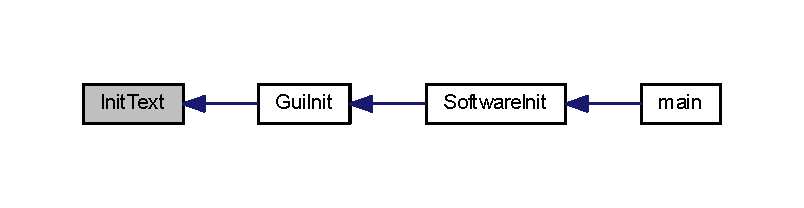
\includegraphics[width=350pt]{group___w_i_d_g_e_t_gac18895bdc14f553f346c2b01e6fcc119_icgraph}
\end{center}
\end{figure}


\hypertarget{group___w_i_d_g_e_t_ga7a6ad9f67f512cb71394be195152a1bc}{\index{\-Widget\-: A\-P\-P Group@{\-Widget\-: A\-P\-P Group}!\-Init\-Value@{\-Init\-Value}}
\index{\-Init\-Value@{\-Init\-Value}!Widget: APP Group@{\-Widget\-: A\-P\-P Group}}
\subsubsection[{\-Init\-Value}]{\setlength{\rightskip}{0pt plus 5cm}void {\bf \-Init\-Value} (
\begin{DoxyParamCaption}
\item[{{\bf u8}}]{x, }
\item[{{\bf u8}}]{y, }
\item[{{\bf u8}}]{dot, }
\item[{char $\ast$}]{str, }
\item[{{\bf \-S\-T\-R\-\_\-\-Value} $\ast$}]{value}
\end{DoxyParamCaption}
)}}\label{group___w_i_d_g_e_t_ga7a6ad9f67f512cb71394be195152a1bc}


初始化数值控件 


\begin{DoxyParams}[1]{\-Parameters}
 & {\em 参数名} & 参数说明 \\
\hline
\mbox{\tt in}  & {\em x} & x轴坐标 \\
\hline
\mbox{\tt in}  & {\em y} & y轴坐标 \\
\hline
\mbox{\tt in}  & {\em dot} & 小数点位数 \\
\hline
\mbox{\tt in}  & {\em str} & 单位字符串 \\
\hline
\mbox{\tt out}  & {\em value} & 数值控件指针 \\
\hline
\end{DoxyParams}

\begin{DoxyRetVals}{\-Return values}
{\em 无} & \\
\hline
\end{DoxyRetVals}
\begin{DoxyParagraph}{使用全局变量 }

\end{DoxyParagraph}
\begin{DoxyNote}{\-Note}
● 执行时间\-: \par
 ● 调用周期\-: 触发调用, 初始化时调用 \par
 ● 可否打断\-: 可以 \par

\end{DoxyNote}
\begin{DoxyParagraph}{注意\-:}
● 无 \par
 
\end{DoxyParagraph}


\-Here is the caller graph for this function\-:\nopagebreak
\begin{figure}[H]
\begin{center}
\leavevmode
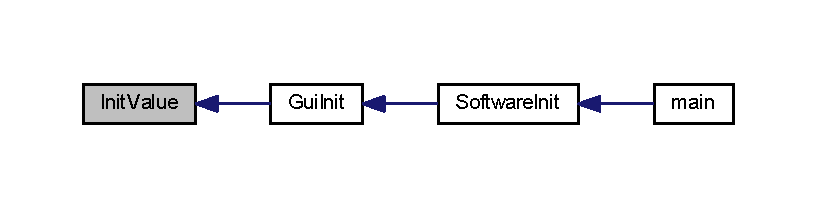
\includegraphics[width=350pt]{group___w_i_d_g_e_t_ga7a6ad9f67f512cb71394be195152a1bc_icgraph}
\end{center}
\end{figure}




\subsection{\-Variable \-Documentation}
\hypertarget{group___w_i_d_g_e_t_ga9cac21b10aac988fd92e2cd2c78a4319}{\index{\-Widget\-: A\-P\-P Group@{\-Widget\-: A\-P\-P Group}!font\-Battery@{font\-Battery}}
\index{font\-Battery@{font\-Battery}!Widget: APP Group@{\-Widget\-: A\-P\-P Group}}
\subsubsection[{font\-Battery}]{\setlength{\rightskip}{0pt plus 5cm}const unsigned char {\bf font\-Battery}\mbox{[}$\,$\mbox{]}\mbox{[}10\mbox{]}}}\label{group___w_i_d_g_e_t_ga9cac21b10aac988fd92e2cd2c78a4319}
{\bfseries \-Initial value\-:}
\begin{DoxyCode}
 
{

{0x00,0xFC,0x04,0x06,0x02,0x02,0x06,0x04,0xFC,0x00},
{0x00,0x7F,0x40,0x40,0x40,0x40,0x40,0x40,0x7F,0x00},

{0x00,0xFC,0x04,0x06,0x02,0x02,0x06,0x04,0xFC,0x00},
{0x00,0x7F,0x70,0x70,0x70,0x70,0x70,0x70,0x7F,0x00},

{0x00,0xFC,0x04,0x06,0x02,0x02,0x06,0x04,0xFC,0x00},
{0x00,0x7F,0x7C,0x7C,0x7C,0x7C,0x7C,0x7C,0x7F,0x00},

{0x00,0xFC,0x04,0x06,0x02,0x02,0x06,0x04,0xFC,0x00},
{0x00,0x7F,0x7F,0x7F,0x7F,0x7F,0x7F,0x7F,0x7F,0x00},

{0x00,0xFC,0xC4,0xC6,0xC2,0xC2,0xC6,0xC4,0xFC,0x00},
{0x00,0x7F,0x7F,0x7F,0x7F,0x7F,0x7F,0x7F,0x7F,0x00},

{0x00,0xFC,0xF4,0xF6,0xF2,0xF2,0xF6,0xF4,0xFC,0x00},
{0x00,0x7F,0x7F,0x7F,0x7F,0x7F,0x7F,0x7F,0x7F,0x00},

{0x00,0xFC,0xFC,0xFE,0xFE,0xFE,0xFE,0xFC,0xFC,0x00},
{0x00,0x7F,0x7F,0x7F,0x7F,0x7F,0x7F,0x7F,0x7F,0x00},

}
\end{DoxyCode}


电量显示图标 

\hypertarget{group___w_i_d_g_e_t_gae789ac73b9f8bf563ff477571af3e532}{\index{\-Widget\-: A\-P\-P Group@{\-Widget\-: A\-P\-P Group}!font\-B\-L\-E@{font\-B\-L\-E}}
\index{font\-B\-L\-E@{font\-B\-L\-E}!Widget: APP Group@{\-Widget\-: A\-P\-P Group}}
\subsubsection[{font\-B\-L\-E}]{\setlength{\rightskip}{0pt plus 5cm}const unsigned char {\bf font\-B\-L\-E}\mbox{[}$\,$\mbox{]}\mbox{[}10\mbox{]}}}\label{group___w_i_d_g_e_t_gae789ac73b9f8bf563ff477571af3e532}
{\bfseries \-Initial value\-:}
\begin{DoxyCode}
 
{

{0x00,0x00,0x00,0x00,0x00,0x00,0x00,0x00,0x00,0x00},
{0x00,0x00,0x00,0x00,0x00,0x00,0x00,0x00,0x00,0x00},

{0x10,0x20,0x40,0xFF,0x82,0x44,0x28,0x10,0x00,0x00},
{0x08,0x04,0x02,0x7F,0x20,0x11,0x0A,0x04,0x00,0x00},
}
\end{DoxyCode}


蓝牙图标 

\hypertarget{group___w_i_d_g_e_t_ga4281d2c990312a449f8115a73da5d4b6}{\index{\-Widget\-: A\-P\-P Group@{\-Widget\-: A\-P\-P Group}!font\-Delay@{font\-Delay}}
\index{font\-Delay@{font\-Delay}!Widget: APP Group@{\-Widget\-: A\-P\-P Group}}
\subsubsection[{font\-Delay}]{\setlength{\rightskip}{0pt plus 5cm}const unsigned char {\bf font\-Delay}\mbox{[}$\,$\mbox{]}\mbox{[}15\mbox{]}}}\label{group___w_i_d_g_e_t_ga4281d2c990312a449f8115a73da5d4b6}
{\bfseries \-Initial value\-:}
\begin{DoxyCode}
 
{

{0x00,0x00,0x00,0x00,0x00,0x00,0x00,0x00,0x00,0x00,0x00,0x00,0x00,0x00,0x00},
{0x00,0x00,0x00,0x00,0x00,0x00,0x00,0x00,0x00,0x00,0x00,0x00,0x00,0x00,0x00},

{0xC0,0x70,0x18,0x0C,0x24,0x46,0x82,0x02,0x02,0x06,0x04,0x0C,0x18,0x70,0xC0},
{0x07,0x1C,0x30,0x60,0x40,0xC0,0x80,0x81,0x81,0xC1,0x41,0x61,0x31,0x1C,0x07},
}
\end{DoxyCode}


时钟图标 

\hypertarget{group___w_i_d_g_e_t_ga7ef23e7312ba1eef34a75bae365cf3e3}{\index{\-Widget\-: A\-P\-P Group@{\-Widget\-: A\-P\-P Group}!font\-Enable@{font\-Enable}}
\index{font\-Enable@{font\-Enable}!Widget: APP Group@{\-Widget\-: A\-P\-P Group}}
\subsubsection[{font\-Enable}]{\setlength{\rightskip}{0pt plus 5cm}const unsigned char {\bf font\-Enable}\mbox{[}$\,$\mbox{]}\mbox{[}8\mbox{]}}}\label{group___w_i_d_g_e_t_ga7ef23e7312ba1eef34a75bae365cf3e3}
{\bfseries \-Initial value\-:}
\begin{DoxyCode}

{
{0x00,0x7F,0x41,0x41,0x41,0x41,0x41,0x7F},

{0x00,0x7F,0x51,0x61,0x51,0x49,0x45,0x7F},

}
\end{DoxyCode}


勾选框图标 

\hypertarget{group___w_i_d_g_e_t_ga934307f74cc38f1062d272ab796d7715}{\index{\-Widget\-: A\-P\-P Group@{\-Widget\-: A\-P\-P Group}!font\-Slide@{font\-Slide}}
\index{font\-Slide@{font\-Slide}!Widget: APP Group@{\-Widget\-: A\-P\-P Group}}
\subsubsection[{font\-Slide}]{\setlength{\rightskip}{0pt plus 5cm}const unsigned char {\bf font\-Slide}\mbox{[}$\,$\mbox{]}\mbox{[}100\mbox{]}}}\label{group___w_i_d_g_e_t_ga934307f74cc38f1062d272ab796d7715}
{\bfseries \-Initial value\-:}
\begin{DoxyCode}
 
{ 
    0x18, 0x18, 0x18, 0x18, 0x18, 0x18, 0x18, 0x18, 0x18, 0x18,
    0x18, 0x18, 0x18, 0x18, 0x18, 0x18, 0x18, 0x18, 0x18, 0x18,
    0x18, 0x18, 0x18, 0x18, 0x18, 0x18, 0x18, 0x18, 0x18, 0x18,
    0x18, 0x18, 0x18, 0x18, 0x18, 0x18, 0x18, 0x18, 0x18, 0x18,
    0x18, 0x18, 0x18, 0x18, 0x18, 0x18, 0x18, 0x18, 0x18, 0x18,
    0x18, 0x18, 0x18, 0x18, 0x18, 0x18, 0x18, 0x18, 0x18, 0x18,
    0x18, 0x18, 0x18, 0x18, 0x18, 0x18, 0x18, 0x18, 0x18, 0x18,
    0x18, 0x18, 0x18, 0x18, 0x18, 0x18, 0x18, 0x18, 0x18, 0x18,
    0x18, 0x18, 0x18, 0x18, 0x18, 0x18, 0x18, 0x18, 0x18, 0x18,
    0x18, 0x18, 0x18, 0x18, 0x18, 0x18, 0x18, 0x18, 0x18, 0x18, 
}
\end{DoxyCode}


进度条图标 

\hypertarget{group___w_i_d_g_e_t_ga934cfdf8aedca0ff9a8794005da8d5e0}{\index{\-Widget\-: A\-P\-P Group@{\-Widget\-: A\-P\-P Group}!font\-Time\-Colon@{font\-Time\-Colon}}
\index{font\-Time\-Colon@{font\-Time\-Colon}!Widget: APP Group@{\-Widget\-: A\-P\-P Group}}
\subsubsection[{font\-Time\-Colon}]{\setlength{\rightskip}{0pt plus 5cm}const unsigned char {\bf font\-Time\-Colon}\mbox{[}$\,$\mbox{]}\mbox{[}16\mbox{]}}}\label{group___w_i_d_g_e_t_ga934cfdf8aedca0ff9a8794005da8d5e0}
{\bfseries \-Initial value\-:}
\begin{DoxyCode}

{
        
{0x00,0x00,0x00,0x00,0x00,0x00,0x00,0x00,0x00,0x00,0x00,0x00,0x00,0x00,0x00,
      0x00},
{0x00,0x00,0x00,0x00,0x00,0xE0,0xF0,0xF0,0xF0,0xF0,0xF0,0xE0,0x00,0x00,0x00,
      0x00},
{0x00,0x00,0x00,0x00,0x00,0x00,0x01,0x01,0x01,0x01,0x01,0x00,0x00,0x00,0x00,
      0x00},
{0x00,0x00,0x00,0x00,0x00,0x00,0x80,0x80,0x80,0x80,0x80,0x00,0x00,0x00,0x00,
      0x00},
{0x00,0x00,0x00,0x00,0x00,0x07,0x0F,0x0F,0x0F,0x0F,0x0F,0x07,0x00,0x00,0x00,
      0x00},
{0x00,0x00,0x00,0x00,0x00,0x00,0x00,0x00,0x00,0x00,0x00,0x00,0x00,0x00,0x00,
      0x00},


{0x00,0x00,0x00,0x00,0x00,0x00,0x00,0x00,0x00,0x00,0x00,0x00,0x00,0x00,0x00,
      0x00},
{0x00,0x00,0x00,0x00,0x00,0x00,0x00,0x00,0x00,0x00,0x00,0x00,0x00,0x00,0x00,
      0x00},
{0x00,0x00,0x00,0x00,0x00,0x00,0x00,0x00,0x00,0x00,0x00,0x00,0x00,0x00,0x00,
      0x00},
{0x00,0x00,0x00,0x00,0x00,0x00,0x00,0x00,0x00,0x00,0x00,0x00,0x00,0x00,0x00,
      0x00},
{0x00,0x00,0x00,0x00,0x00,0x00,0x00,0x00,0x00,0x00,0x00,0x00,0x00,0x00,0x00,
      0x00},
{0x00,0x00,0x00,0x00,0x00,0x00,0x00,0x00,0x00,0x00,0x00,0x00,0x00,0x00,0x00,
      0x00},


}
\end{DoxyCode}


时间显示用的冒号 


\hypertarget{group___p_o_w_e_r}{\section{\-Power\-: \-A\-P\-P \-Group}
\label{group___p_o_w_e_r}\index{\-Power\-: A\-P\-P Group@{\-Power\-: A\-P\-P Group}}
}
\subsection*{\-Data \-Structures}
\begin{DoxyCompactItemize}
\item 
struct \hyperlink{struct_s_t_r___power}{\-S\-T\-R\-\_\-\-Power}
\begin{DoxyCompactList}\small\item\em 能耗控制结构体 \end{DoxyCompactList}\end{DoxyCompactItemize}
\subsection*{\-Enumerations}
\begin{DoxyCompactItemize}
\item 
enum \hyperlink{group___p_o_w_e_r_ga91eadf2d6779b6b61c085ca51be8e7fd}{\-E\-N\-U\-M\-\_\-\-Sys\-Stt} \{ \hyperlink{group___p_o_w_e_r_gga91eadf2d6779b6b61c085ca51be8e7fda50d1448013c6f17125caee18aa418af7}{\-N\-O\-R\-M\-A\-L} =  0, 
\hyperlink{group___p_o_w_e_r_gga91eadf2d6779b6b61c085ca51be8e7fda2a4641f94255505f52278dbcf43bb2dd}{\-O\-L\-E\-D\-O\-F\-F} =  1, 
\hyperlink{group___p_o_w_e_r_gga91eadf2d6779b6b61c085ca51be8e7fdad6137abebe4fdc59e2f0f2c84bdbe3fa}{\-S\-L\-E\-E\-P} =  2
 \}
\begin{DoxyCompactList}\small\item\em 系统功耗控制状态 \end{DoxyCompactList}\end{DoxyCompactItemize}
\subsection*{\-Functions}
\begin{DoxyCompactItemize}
\item 
void \hyperlink{group___p_o_w_e_r_ga11958ae64176cfbdd9f0fbcf81123c8d}{\-Power\-Manage} (\hyperlink{struct_s_t_r___power}{\-S\-T\-R\-\_\-\-Power} $\ast$power)
\begin{DoxyCompactList}\small\item\em 能耗管理函数 \end{DoxyCompactList}\end{DoxyCompactItemize}
\subsection*{\-Variables}
\begin{DoxyCompactItemize}
\item 
\hypertarget{group___p_o_w_e_r_gaaecab9adfce41ce80a1ff422608e52b1}{\hyperlink{struct_s_t_r___power}{\-S\-T\-R\-\_\-\-Power} \hyperlink{group___p_o_w_e_r_gaaecab9adfce41ce80a1ff422608e52b1}{\-Power}}\label{group___p_o_w_e_r_gaaecab9adfce41ce80a1ff422608e52b1}

\begin{DoxyCompactList}\small\item\em 能耗控制结构体 \end{DoxyCompactList}\item 
\hypertarget{group___p_o_w_e_r_gaaecab9adfce41ce80a1ff422608e52b1}{\hyperlink{struct_s_t_r___power}{\-S\-T\-R\-\_\-\-Power} \hyperlink{group___p_o_w_e_r_gaaecab9adfce41ce80a1ff422608e52b1}{\-Power}}\label{group___p_o_w_e_r_gaaecab9adfce41ce80a1ff422608e52b1}

\begin{DoxyCompactList}\small\item\em 能耗控制结构体 \end{DoxyCompactList}\end{DoxyCompactItemize}


\subsection{\-Enumeration \-Type \-Documentation}
\hypertarget{group___p_o_w_e_r_ga91eadf2d6779b6b61c085ca51be8e7fd}{\index{\-Power\-: A\-P\-P Group@{\-Power\-: A\-P\-P Group}!\-E\-N\-U\-M\-\_\-\-Sys\-Stt@{\-E\-N\-U\-M\-\_\-\-Sys\-Stt}}
\index{\-E\-N\-U\-M\-\_\-\-Sys\-Stt@{\-E\-N\-U\-M\-\_\-\-Sys\-Stt}!Power: APP Group@{\-Power\-: A\-P\-P Group}}
\subsubsection[{\-E\-N\-U\-M\-\_\-\-Sys\-Stt}]{\setlength{\rightskip}{0pt plus 5cm}enum {\bf \-E\-N\-U\-M\-\_\-\-Sys\-Stt}}}\label{group___p_o_w_e_r_ga91eadf2d6779b6b61c085ca51be8e7fd}


系统功耗控制状态 

\begin{Desc}
\item[\-Enumerator\-: ]\par
\begin{description}
\index{\-N\-O\-R\-M\-A\-L@{\-N\-O\-R\-M\-A\-L}!\-Power\-: A\-P\-P Group@{\-Power\-: A\-P\-P Group}}\index{\-Power\-: A\-P\-P Group@{\-Power\-: A\-P\-P Group}!\-N\-O\-R\-M\-A\-L@{\-N\-O\-R\-M\-A\-L}}\item[{\em 
\hypertarget{group___p_o_w_e_r_gga91eadf2d6779b6b61c085ca51be8e7fda50d1448013c6f17125caee18aa418af7}{\-N\-O\-R\-M\-A\-L}\label{group___p_o_w_e_r_gga91eadf2d6779b6b61c085ca51be8e7fda50d1448013c6f17125caee18aa418af7}
}]正常模式 \index{\-O\-L\-E\-D\-O\-F\-F@{\-O\-L\-E\-D\-O\-F\-F}!\-Power\-: A\-P\-P Group@{\-Power\-: A\-P\-P Group}}\index{\-Power\-: A\-P\-P Group@{\-Power\-: A\-P\-P Group}!\-O\-L\-E\-D\-O\-F\-F@{\-O\-L\-E\-D\-O\-F\-F}}\item[{\em 
\hypertarget{group___p_o_w_e_r_gga91eadf2d6779b6b61c085ca51be8e7fda2a4641f94255505f52278dbcf43bb2dd}{\-O\-L\-E\-D\-O\-F\-F}\label{group___p_o_w_e_r_gga91eadf2d6779b6b61c085ca51be8e7fda2a4641f94255505f52278dbcf43bb2dd}
}]熄屏模式 \index{\-S\-L\-E\-E\-P@{\-S\-L\-E\-E\-P}!\-Power\-: A\-P\-P Group@{\-Power\-: A\-P\-P Group}}\index{\-Power\-: A\-P\-P Group@{\-Power\-: A\-P\-P Group}!\-S\-L\-E\-E\-P@{\-S\-L\-E\-E\-P}}\item[{\em 
\hypertarget{group___p_o_w_e_r_gga91eadf2d6779b6b61c085ca51be8e7fdad6137abebe4fdc59e2f0f2c84bdbe3fa}{\-S\-L\-E\-E\-P}\label{group___p_o_w_e_r_gga91eadf2d6779b6b61c085ca51be8e7fdad6137abebe4fdc59e2f0f2c84bdbe3fa}
}]睡眠模式 \end{description}
\end{Desc}



\subsection{\-Function \-Documentation}
\hypertarget{group___p_o_w_e_r_ga11958ae64176cfbdd9f0fbcf81123c8d}{\index{\-Power\-: A\-P\-P Group@{\-Power\-: A\-P\-P Group}!\-Power\-Manage@{\-Power\-Manage}}
\index{\-Power\-Manage@{\-Power\-Manage}!Power: APP Group@{\-Power\-: A\-P\-P Group}}
\subsubsection[{\-Power\-Manage}]{\setlength{\rightskip}{0pt plus 5cm}void {\bf \-Power\-Manage} (
\begin{DoxyParamCaption}
\item[{{\bf \-S\-T\-R\-\_\-\-Power} $\ast$}]{power}
\end{DoxyParamCaption}
)}}\label{group___p_o_w_e_r_ga11958ae64176cfbdd9f0fbcf81123c8d}


能耗管理函数 


\begin{DoxyParams}[1]{\-Parameters}
 & {\em 参数名} & 参数说明 \\
\hline
\mbox{\tt in}  & {\em power} & 能耗管理结构体指针 \\
\hline
\end{DoxyParams}

\begin{DoxyRetVals}{\-Return values}
{\em 无} & \\
\hline
\end{DoxyRetVals}
\begin{DoxyParagraph}{使用全局变量 }

\end{DoxyParagraph}
\begin{DoxyNote}{\-Note}
● 执行时间\-: \par
 ● 调用周期\-: 100ms \par
 ● 可否打断\-: 可以 \par

\end{DoxyNote}
\begin{DoxyParagraph}{注意\-:}
● 无 \par
 
\end{DoxyParagraph}


\-Here is the call graph for this function\-:\nopagebreak
\begin{figure}[H]
\begin{center}
\leavevmode
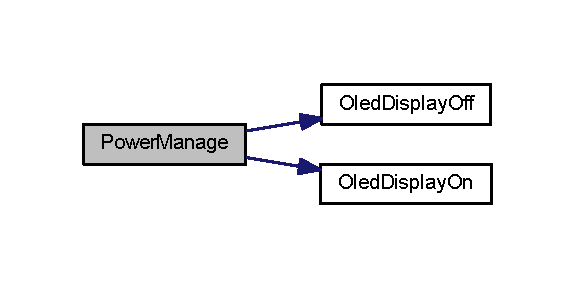
\includegraphics[width=276pt]{group___p_o_w_e_r_ga11958ae64176cfbdd9f0fbcf81123c8d_cgraph}
\end{center}
\end{figure}



\hypertarget{group___p_r_o_t_o_c_o_l}{\section{\-Protocol\-: \-A\-P\-P \-Group}
\label{group___p_r_o_t_o_c_o_l}\index{\-Protocol\-: A\-P\-P Group@{\-Protocol\-: A\-P\-P Group}}
}
\subsection*{\-Functions}
\begin{DoxyCompactItemize}
\item 
void \hyperlink{group___p_r_o_t_o_c_o_l_ga996a71b9cf063aedf04cff5d79b4c66e}{\-Uart\-Decode} (\hyperlink{struct_s_t_r___uart}{\-S\-T\-R\-\_\-\-Uart} $\ast$uart)
\begin{DoxyCompactList}\small\item\em 串口数据解析函数 \end{DoxyCompactList}\end{DoxyCompactItemize}


\subsection{\-Function \-Documentation}
\hypertarget{group___p_r_o_t_o_c_o_l_ga996a71b9cf063aedf04cff5d79b4c66e}{\index{\-Protocol\-: A\-P\-P Group@{\-Protocol\-: A\-P\-P Group}!\-Uart\-Decode@{\-Uart\-Decode}}
\index{\-Uart\-Decode@{\-Uart\-Decode}!Protocol: APP Group@{\-Protocol\-: A\-P\-P Group}}
\subsubsection[{\-Uart\-Decode}]{\setlength{\rightskip}{0pt plus 5cm}void {\bf \-Uart\-Decode} (
\begin{DoxyParamCaption}
\item[{{\bf \-S\-T\-R\-\_\-\-Uart} $\ast$}]{uart}
\end{DoxyParamCaption}
)}}\label{group___p_r_o_t_o_c_o_l_ga996a71b9cf063aedf04cff5d79b4c66e}


串口数据解析函数 


\begin{DoxyParams}[1]{\-Parameters}
 & {\em 参数名} & 参数说明 \\
\hline
\mbox{\tt in}  & {\em uart} & 串口结构体指针 \\
\hline
\end{DoxyParams}

\begin{DoxyRetVals}{\-Return values}
{\em 无} & \\
\hline
\end{DoxyRetVals}
\begin{DoxyParagraph}{使用全局变量 }

\end{DoxyParagraph}
\begin{DoxyNote}{\-Note}
● 执行时间\-: \par
 ● 调用周期\-: 4ms \par
 ● 可否打断\-: 可以 \par

\end{DoxyNote}
\begin{DoxyParagraph}{注意\-:}
● 无 \par
 
\end{DoxyParagraph}

\hypertarget{group___t_a_s_k}{\section{\-Task\-: \-A\-P\-P \-Group}
\label{group___t_a_s_k}\index{\-Task\-: A\-P\-P Group@{\-Task\-: A\-P\-P Group}}
}
\subsection*{\-Functions}
\begin{DoxyCompactItemize}
\item 
void \hyperlink{group___t_a_s_k_gad7f568b58dcae6573d84519c01f70516}{\-Task} (void)
\begin{DoxyCompactList}\small\item\em 任务分派函数 \end{DoxyCompactList}\end{DoxyCompactItemize}


\subsection{\-Function \-Documentation}
\hypertarget{group___t_a_s_k_gad7f568b58dcae6573d84519c01f70516}{\index{\-Task\-: A\-P\-P Group@{\-Task\-: A\-P\-P Group}!\-Task@{\-Task}}
\index{\-Task@{\-Task}!Task: APP Group@{\-Task\-: A\-P\-P Group}}
\subsubsection[{\-Task}]{\setlength{\rightskip}{0pt plus 5cm}void {\bf \-Task} (
\begin{DoxyParamCaption}
\item[{void}]{}
\end{DoxyParamCaption}
)}}\label{group___t_a_s_k_gad7f568b58dcae6573d84519c01f70516}


任务分派函数 


\begin{DoxyParams}{\-Parameters}
{\em 参数名} & 参数说明 \\
\hline
{\em 无} & \\
\hline
\end{DoxyParams}

\begin{DoxyRetVals}{\-Return values}
{\em 无} & \\
\hline
\end{DoxyRetVals}
\begin{DoxyNote}{\-Note}
● 调用周期\-: 500us调用\par
 $\ast$ 
\end{DoxyNote}
\begin{DoxyParagraph}{注意\-:}
● \par
 
\end{DoxyParagraph}


\-Here is the caller graph for this function\-:\nopagebreak
\begin{figure}[H]
\begin{center}
\leavevmode
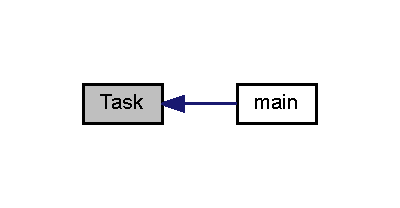
\includegraphics[width=192pt]{group___t_a_s_k_gad7f568b58dcae6573d84519c01f70516_icgraph}
\end{center}
\end{figure}



\hypertarget{group___b_s_p}{\section{\-Bsp\-: \-B\-S\-P \-Group}
\label{group___b_s_p}\index{\-Bsp\-: B\-S\-P Group@{\-Bsp\-: B\-S\-P Group}}
}
\subsection*{\-Typedefs}
\begin{DoxyCompactItemize}
\item 
\hypertarget{group___b_s_p_gaed742c436da53c1080638ce6ef7d13de}{typedef unsigned char \hyperlink{group___b_s_p_gaed742c436da53c1080638ce6ef7d13de}{u8}}\label{group___b_s_p_gaed742c436da53c1080638ce6ef7d13de}

\begin{DoxyCompactList}\small\item\em 8位无符号整形 \end{DoxyCompactList}\item 
\hypertarget{group___b_s_p_ga9e6c91d77e24643b888dbd1a1a590054}{typedef unsigned short \hyperlink{group___b_s_p_ga9e6c91d77e24643b888dbd1a1a590054}{u16}}\label{group___b_s_p_ga9e6c91d77e24643b888dbd1a1a590054}

\begin{DoxyCompactList}\small\item\em 16位无符号整形 \end{DoxyCompactList}\item 
\hypertarget{group___b_s_p_ga10e94b422ef0c20dcdec20d31a1f5049}{typedef unsigned int \hyperlink{group___b_s_p_ga10e94b422ef0c20dcdec20d31a1f5049}{u32}}\label{group___b_s_p_ga10e94b422ef0c20dcdec20d31a1f5049}

\begin{DoxyCompactList}\small\item\em 32位无符号整形 \end{DoxyCompactList}\item 
\hypertarget{group___b_s_p_gad758b7a5c3f18ed79d2fcd23d9f16357}{typedef unsigned long long \hyperlink{group___b_s_p_gad758b7a5c3f18ed79d2fcd23d9f16357}{u64}}\label{group___b_s_p_gad758b7a5c3f18ed79d2fcd23d9f16357}

\begin{DoxyCompactList}\small\item\em 64位无符号整形 \end{DoxyCompactList}\item 
\hypertarget{group___b_s_p_ga151f780fb455885061d3b77ec1c90c03}{typedef signed char \hyperlink{group___b_s_p_ga151f780fb455885061d3b77ec1c90c03}{s8}}\label{group___b_s_p_ga151f780fb455885061d3b77ec1c90c03}

\begin{DoxyCompactList}\small\item\em 8位有符号整形 \end{DoxyCompactList}\item 
\hypertarget{group___b_s_p_ga5ffa4f640862b25ba6d4f635b78bdbe1}{typedef signed short \hyperlink{group___b_s_p_ga5ffa4f640862b25ba6d4f635b78bdbe1}{s16}}\label{group___b_s_p_ga5ffa4f640862b25ba6d4f635b78bdbe1}

\begin{DoxyCompactList}\small\item\em 16位有符号整形 \end{DoxyCompactList}\item 
\hypertarget{group___b_s_p_ga0ce6887c26c1c49ad3be5710dd42bfd6}{typedef signed int \hyperlink{group___b_s_p_ga0ce6887c26c1c49ad3be5710dd42bfd6}{s32}}\label{group___b_s_p_ga0ce6887c26c1c49ad3be5710dd42bfd6}

\begin{DoxyCompactList}\small\item\em 32位有符号整形 \end{DoxyCompactList}\item 
\hypertarget{group___b_s_p_ga4258bfb2c3a440d06c4aaa3c2b450dde}{typedef signed long long \hyperlink{group___b_s_p_ga4258bfb2c3a440d06c4aaa3c2b450dde}{s64}}\label{group___b_s_p_ga4258bfb2c3a440d06c4aaa3c2b450dde}

\begin{DoxyCompactList}\small\item\em 64位有符号整形 \end{DoxyCompactList}\end{DoxyCompactItemize}
\subsection*{\-Functions}
\begin{DoxyCompactItemize}
\item 
void \hyperlink{group___b_s_p_ga93f514700ccf00d08dbdcff7f1224eb2}{\-System\-Init} (void)
\begin{DoxyCompactList}\small\item\em 硬件初始函数 \end{DoxyCompactList}\end{DoxyCompactItemize}


\subsection{\-Function \-Documentation}
\hypertarget{group___b_s_p_ga93f514700ccf00d08dbdcff7f1224eb2}{\index{\-Bsp\-: B\-S\-P Group@{\-Bsp\-: B\-S\-P Group}!\-System\-Init@{\-System\-Init}}
\index{\-System\-Init@{\-System\-Init}!Bsp: BSP Group@{\-Bsp\-: B\-S\-P Group}}
\subsubsection[{\-System\-Init}]{\setlength{\rightskip}{0pt plus 5cm}void {\bf \-System\-Init} (
\begin{DoxyParamCaption}
\item[{void}]{}
\end{DoxyParamCaption}
)}}\label{group___b_s_p_ga93f514700ccf00d08dbdcff7f1224eb2}


硬件初始函数 

硬件初始化函数


\begin{DoxyParams}{\-Parameters}
{\em 参数名} & 参数说明 \\
\hline
{\em 无} & \\
\hline
\end{DoxyParams}

\begin{DoxyRetVals}{\-Return values}
{\em 无} & \\
\hline
\end{DoxyRetVals}
\begin{DoxyParagraph}{使用全局变量 }

\end{DoxyParagraph}
\begin{DoxyNote}{\-Note}
● 执行时间\-: \par
 ● 调用周期\-: 触发调用, 初始化时调用 \par
 ● 可否打断\-: 可以 \par

\end{DoxyNote}
\begin{DoxyParagraph}{注意\-:}
● 无 \par
 
\end{DoxyParagraph}


\-Here is the call graph for this function\-:\nopagebreak
\begin{figure}[H]
\begin{center}
\leavevmode
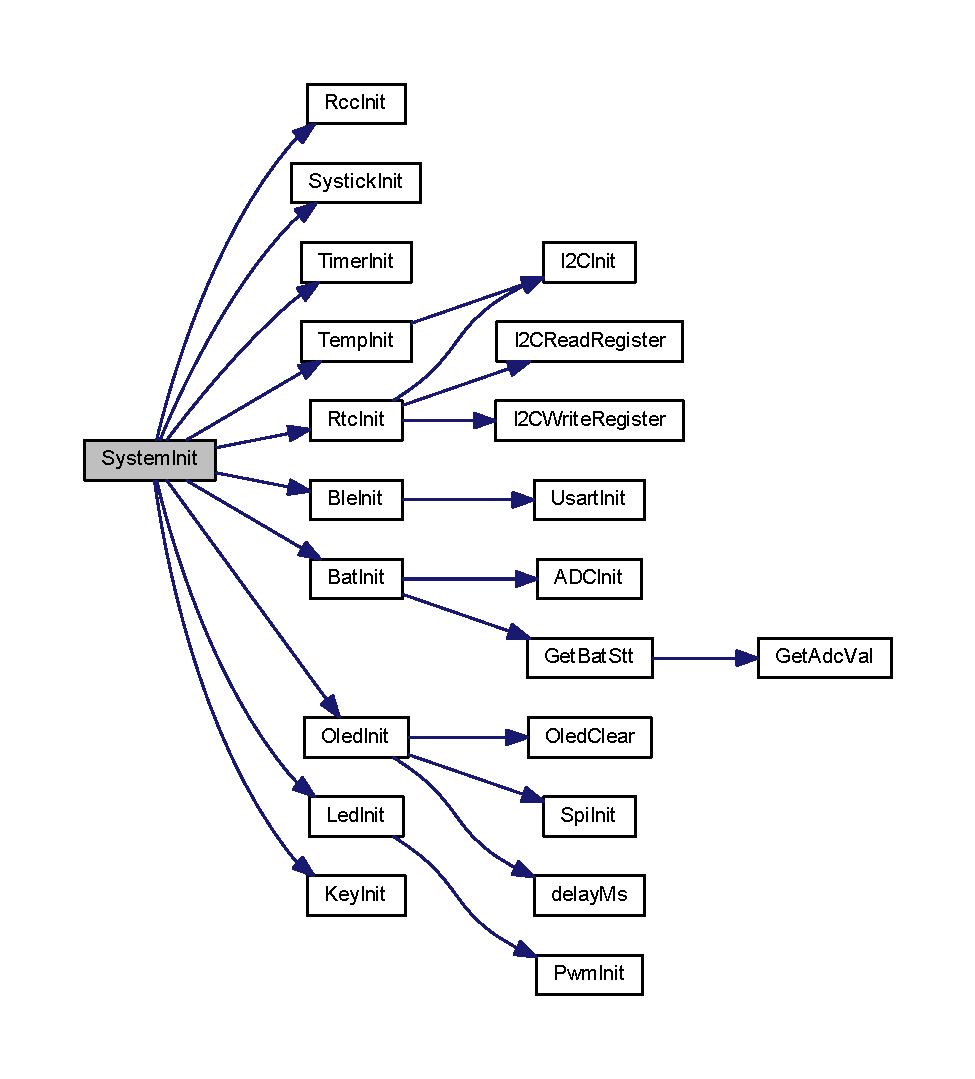
\includegraphics[width=350pt]{group___b_s_p_ga93f514700ccf00d08dbdcff7f1224eb2_cgraph}
\end{center}
\end{figure}




\-Here is the caller graph for this function\-:\nopagebreak
\begin{figure}[H]
\begin{center}
\leavevmode
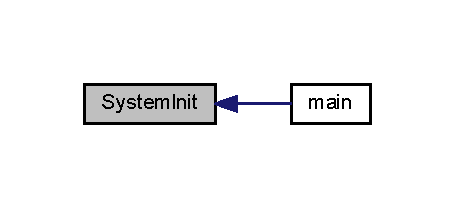
\includegraphics[width=218pt]{group___b_s_p_ga93f514700ccf00d08dbdcff7f1224eb2_icgraph}
\end{center}
\end{figure}



\hypertarget{group___b_e_t_t_e_r_y}{\section{\-Bsp\-Battery\-: \-B\-S\-P \-Group}
\label{group___b_e_t_t_e_r_y}\index{\-Bsp\-Battery\-: B\-S\-P Group@{\-Bsp\-Battery\-: B\-S\-P Group}}
}
\subsection*{\-Data \-Structures}
\begin{DoxyCompactItemize}
\item 
union \hyperlink{union_u_n___bat_stt}{\-U\-N\-\_\-\-Bat\-Stt}
\begin{DoxyCompactList}\small\item\em 电池状态联合体 \end{DoxyCompactList}\item 
struct \hyperlink{struct_s_t_r___b_a_t_t_e_r_y}{\-S\-T\-R\-\_\-\-B\-A\-T\-T\-E\-R\-Y}
\begin{DoxyCompactList}\small\item\em 电池信息结构体 \end{DoxyCompactList}\end{DoxyCompactItemize}
\subsection*{\-Functions}
\begin{DoxyCompactItemize}
\item 
void \hyperlink{group___b_e_t_t_e_r_y_ga9daea963d01ab321f8f2cb6f2b8932b2}{\-Bat\-Init} (void)
\begin{DoxyCompactList}\small\item\em 电池检测初始化函数 \end{DoxyCompactList}\item 
void \hyperlink{group___b_e_t_t_e_r_y_gad11b24ac1b2d2f4ad3c24201b9c7a244}{\-Get\-Bat\-Stt} (\hyperlink{struct_s_t_r___b_a_t_t_e_r_y}{\-S\-T\-R\-\_\-\-B\-A\-T\-T\-E\-R\-Y} $\ast$bat)
\begin{DoxyCompactList}\small\item\em 更新电池状态函数 \end{DoxyCompactList}\end{DoxyCompactItemize}
\subsection*{\-Variables}
\begin{DoxyCompactItemize}
\item 
\hypertarget{group___b_e_t_t_e_r_y_gab5241bc290b684da54ca6c714fc4bc00}{\hyperlink{struct_s_t_r___b_a_t_t_e_r_y}{\-S\-T\-R\-\_\-\-B\-A\-T\-T\-E\-R\-Y} \hyperlink{group___b_e_t_t_e_r_y_gab5241bc290b684da54ca6c714fc4bc00}{\-Bat}}\label{group___b_e_t_t_e_r_y_gab5241bc290b684da54ca6c714fc4bc00}

\begin{DoxyCompactList}\small\item\em 电池信息结构体 \end{DoxyCompactList}\item 
\hypertarget{group___b_e_t_t_e_r_y_gab5241bc290b684da54ca6c714fc4bc00}{\hyperlink{struct_s_t_r___b_a_t_t_e_r_y}{\-S\-T\-R\-\_\-\-B\-A\-T\-T\-E\-R\-Y} \hyperlink{group___b_e_t_t_e_r_y_gab5241bc290b684da54ca6c714fc4bc00}{\-Bat}}\label{group___b_e_t_t_e_r_y_gab5241bc290b684da54ca6c714fc4bc00}

\begin{DoxyCompactList}\small\item\em 电池信息结构体 \end{DoxyCompactList}\end{DoxyCompactItemize}


\subsection{\-Function \-Documentation}
\hypertarget{group___b_e_t_t_e_r_y_ga9daea963d01ab321f8f2cb6f2b8932b2}{\index{\-Bsp\-Battery\-: B\-S\-P Group@{\-Bsp\-Battery\-: B\-S\-P Group}!\-Bat\-Init@{\-Bat\-Init}}
\index{\-Bat\-Init@{\-Bat\-Init}!BspBattery: BSP Group@{\-Bsp\-Battery\-: B\-S\-P Group}}
\subsubsection[{\-Bat\-Init}]{\setlength{\rightskip}{0pt plus 5cm}void {\bf \-Bat\-Init} (
\begin{DoxyParamCaption}
\item[{void}]{}
\end{DoxyParamCaption}
)}}\label{group___b_e_t_t_e_r_y_ga9daea963d01ab321f8f2cb6f2b8932b2}


电池检测初始化函数 

电池状态检测初始化


\begin{DoxyParams}{\-Parameters}
{\em 参数名} & 参数说明 \\
\hline
{\em 无} & \\
\hline
\end{DoxyParams}

\begin{DoxyRetVals}{\-Return values}
{\em 无} & \\
\hline
\end{DoxyRetVals}
\begin{DoxyParagraph}{使用全局变量 }

\end{DoxyParagraph}
\begin{DoxyNote}{\-Note}
● 执行时间\-: \par
 ● 调用周期\-: 触发调用, 初始化时调用 \par
 ● 可否打断\-: 可以 \par

\end{DoxyNote}
\begin{DoxyParagraph}{注意\-:}
● 无 \par
 
\end{DoxyParagraph}


\-Here is the call graph for this function\-:\nopagebreak
\begin{figure}[H]
\begin{center}
\leavevmode
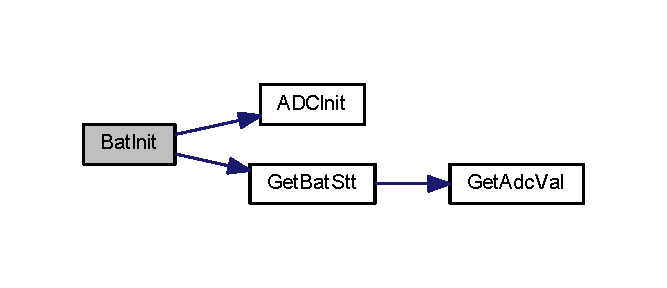
\includegraphics[width=320pt]{group___b_e_t_t_e_r_y_ga9daea963d01ab321f8f2cb6f2b8932b2_cgraph}
\end{center}
\end{figure}




\-Here is the caller graph for this function\-:\nopagebreak
\begin{figure}[H]
\begin{center}
\leavevmode
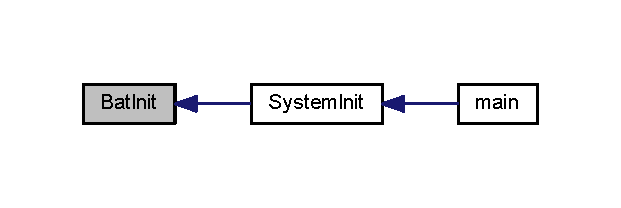
\includegraphics[width=298pt]{group___b_e_t_t_e_r_y_ga9daea963d01ab321f8f2cb6f2b8932b2_icgraph}
\end{center}
\end{figure}


\hypertarget{group___b_e_t_t_e_r_y_gad11b24ac1b2d2f4ad3c24201b9c7a244}{\index{\-Bsp\-Battery\-: B\-S\-P Group@{\-Bsp\-Battery\-: B\-S\-P Group}!\-Get\-Bat\-Stt@{\-Get\-Bat\-Stt}}
\index{\-Get\-Bat\-Stt@{\-Get\-Bat\-Stt}!BspBattery: BSP Group@{\-Bsp\-Battery\-: B\-S\-P Group}}
\subsubsection[{\-Get\-Bat\-Stt}]{\setlength{\rightskip}{0pt plus 5cm}void {\bf \-Get\-Bat\-Stt} (
\begin{DoxyParamCaption}
\item[{{\bf \-S\-T\-R\-\_\-\-B\-A\-T\-T\-E\-R\-Y} $\ast$}]{bat}
\end{DoxyParamCaption}
)}}\label{group___b_e_t_t_e_r_y_gad11b24ac1b2d2f4ad3c24201b9c7a244}


更新电池状态函数 

更新电池状态


\begin{DoxyParams}[1]{\-Parameters}
 & {\em 参数名} & 参数说明 \\
\hline
\mbox{\tt in}  & {\em bat} & 电池状态结构体指针 \\
\hline
\end{DoxyParams}

\begin{DoxyRetVals}{\-Return values}
{\em 无} & \\
\hline
\end{DoxyRetVals}
\begin{DoxyParagraph}{使用全局变量 }

\end{DoxyParagraph}
\begin{DoxyNote}{\-Note}
● 执行时间\-: \par
 ● 调用周期\-: 100ms \par
 ● 可否打断\-: 可以 \par

\end{DoxyNote}
\begin{DoxyParagraph}{注意\-:}
● 无 \par
 
\end{DoxyParagraph}


\-Here is the call graph for this function\-:\nopagebreak
\begin{figure}[H]
\begin{center}
\leavevmode
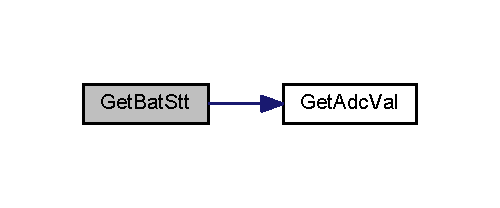
\includegraphics[width=240pt]{group___b_e_t_t_e_r_y_gad11b24ac1b2d2f4ad3c24201b9c7a244_cgraph}
\end{center}
\end{figure}




\-Here is the caller graph for this function\-:\nopagebreak
\begin{figure}[H]
\begin{center}
\leavevmode
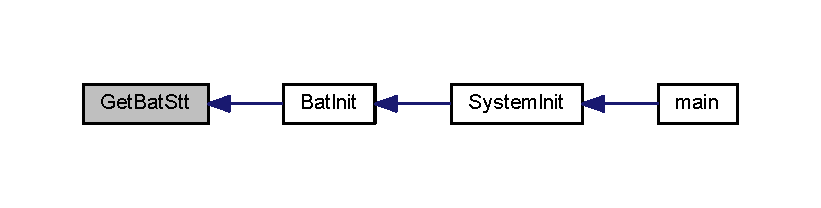
\includegraphics[width=350pt]{group___b_e_t_t_e_r_y_gad11b24ac1b2d2f4ad3c24201b9c7a244_icgraph}
\end{center}
\end{figure}



\hypertarget{group___b_l_e}{\section{\-Bsp\-Ble\-: \-B\-S\-P \-Group}
\label{group___b_l_e}\index{\-Bsp\-Ble\-: B\-S\-P Group@{\-Bsp\-Ble\-: B\-S\-P Group}}
}
\subsection*{\-Data \-Structures}
\begin{DoxyCompactItemize}
\item 
struct \hyperlink{struct_s_t_r___ble_msg}{\-S\-T\-R\-\_\-\-Ble\-Msg}
\begin{DoxyCompactList}\small\item\em 发送缓冲区中报文数量 \end{DoxyCompactList}\item 
struct \hyperlink{struct_s_t_r___ble}{\-S\-T\-R\-\_\-\-Ble}
\begin{DoxyCompactList}\small\item\em 低功耗蓝牙结构体 \end{DoxyCompactList}\end{DoxyCompactItemize}
\subsection*{\-Defines}
\begin{DoxyCompactItemize}
\item 
\hypertarget{group___b_l_e_gaa5ebd183ec26cf40bb11aa48a6b51349}{\#define \hyperlink{group___b_l_e_gaa5ebd183ec26cf40bb11aa48a6b51349}{\-B\-L\-E\-\_\-\-N\-V\-I\-C\-\_\-\-P\-R\-I\-O}~15;}\label{group___b_l_e_gaa5ebd183ec26cf40bb11aa48a6b51349}

\begin{DoxyCompactList}\small\item\em 蓝牙连接中断优先级,这里蓝牙连接优先级和下键共用一个中断, 故优先级相同 \end{DoxyCompactList}\item 
\hypertarget{group___b_l_e_ga404ec81438167db1999e16f77f79760d}{\#define \hyperlink{group___b_l_e_ga404ec81438167db1999e16f77f79760d}{\-B\-Y\-T\-E\-S\-\_\-\-P\-E\-R\-\_\-\-M\-S\-G}~20}\label{group___b_l_e_ga404ec81438167db1999e16f77f79760d}

\begin{DoxyCompactList}\small\item\em 每条报文缓存的大小 \end{DoxyCompactList}\item 
\#define \hyperlink{group___b_l_e_gaf5f8c77ba9a9819251362bc1d7f5f045}{\-B\-L\-E\-\_\-\-S\-E\-N\-D\-\_\-\-I\-D\-L\-E}~0
\begin{DoxyCompactList}\small\item\em 蓝牙发送状态 \end{DoxyCompactList}\item 
\hypertarget{group___b_l_e_gaff49a99d98227ed29cbb3f2776daded9}{\#define \hyperlink{group___b_l_e_gaff49a99d98227ed29cbb3f2776daded9}{\-B\-L\-E\-\_\-\-S\-E\-N\-D\-\_\-\-S\-T\-A\-R\-T}~1}\label{group___b_l_e_gaff49a99d98227ed29cbb3f2776daded9}

\begin{DoxyCompactList}\small\item\em 等待发送引脚置低 \end{DoxyCompactList}\item 
\hypertarget{group___b_l_e_ga18ddb70766e02bd63fe66869f9988fca}{\#define \hyperlink{group___b_l_e_ga18ddb70766e02bd63fe66869f9988fca}{\-B\-L\-E\-\_\-\-S\-E\-N\-D\-\_\-\-P\-R\-O\-C}~2}\label{group___b_l_e_ga18ddb70766e02bd63fe66869f9988fca}

\begin{DoxyCompactList}\small\item\em 正在发送 \end{DoxyCompactList}\item 
\hypertarget{group___b_l_e_gab8a7913edcd2e4a7616a5362354e7824}{\#define \hyperlink{group___b_l_e_gab8a7913edcd2e4a7616a5362354e7824}{\-B\-L\-E\-\_\-\-S\-E\-N\-D\-\_\-\-E\-N\-D}~3}\label{group___b_l_e_gab8a7913edcd2e4a7616a5362354e7824}

\begin{DoxyCompactList}\small\item\em 发送完成,等待发送引脚置高 \end{DoxyCompactList}\end{DoxyCompactItemize}
\subsection*{\-Functions}
\begin{DoxyCompactItemize}
\item 
void \hyperlink{group___b_l_e_gad65e0136086cff966fcbd14a10a8a313}{\-Ble\-Init} (void)
\begin{DoxyCompactList}\small\item\em 温度传感器初始化函数 \end{DoxyCompactList}\item 
void \hyperlink{group___b_l_e_ga916dc062a2f77f89cce44866507bdf52}{\-Ble\-Cmd} (\hyperlink{group___b_s_p_gaed742c436da53c1080638ce6ef7d13de}{u8} new\-State)
\begin{DoxyCompactList}\small\item\em 初始化\-U\-A\-R\-T,使用uart1+\-D\-M\-A,按\-R\-T\-U格式收发数据 \end{DoxyCompactList}\item 
\hyperlink{group___b_s_p_gaed742c436da53c1080638ce6ef7d13de}{u8} \hyperlink{group___b_l_e_ga3fc122f9e39ecffe66a227b87d6051eb}{\-Push\-Send\-Buf} (\hyperlink{group___b_s_p_gaed742c436da53c1080638ce6ef7d13de}{u8} $\ast$data, \hyperlink{group___b_s_p_gaed742c436da53c1080638ce6ef7d13de}{u8} len)
\begin{DoxyCompactList}\small\item\em 将需要发送的数据写入缓冲区 \end{DoxyCompactList}\item 
void \hyperlink{group___b_l_e_ga0c4cf6eee7dc11b12abf30972e242b05}{\-Ble\-Send} (void)
\begin{DoxyCompactList}\small\item\em 蓝牙发送状态机 \end{DoxyCompactList}\item 
void \hyperlink{group___b_l_e_ga738473a5b43f6c92b80ce1d3d6f77ed9}{\-E\-X\-T\-I15\-\_\-10\-\_\-\-I\-R\-Q\-Handler} (void)
\begin{DoxyCompactList}\small\item\em 10$\sim$15通道外部中断处理函数 \end{DoxyCompactList}\end{DoxyCompactItemize}
\subsection*{\-Variables}
\begin{DoxyCompactItemize}
\item 
\hypertarget{group___b_l_e_gabe0f82c09c4ace8e0767f4b4ab756c0a}{\hyperlink{struct_s_t_r___ble}{\-S\-T\-R\-\_\-\-Ble} \hyperlink{group___b_l_e_gabe0f82c09c4ace8e0767f4b4ab756c0a}{\-Ble} = \{0,\}}\label{group___b_l_e_gabe0f82c09c4ace8e0767f4b4ab756c0a}

\begin{DoxyCompactList}\small\item\em 低功耗蓝牙结构体 \end{DoxyCompactList}\item 
\hypertarget{group___b_l_e_gabe0f82c09c4ace8e0767f4b4ab756c0a}{\hyperlink{struct_s_t_r___ble}{\-S\-T\-R\-\_\-\-Ble} \hyperlink{group___b_l_e_gabe0f82c09c4ace8e0767f4b4ab756c0a}{\-Ble}}\label{group___b_l_e_gabe0f82c09c4ace8e0767f4b4ab756c0a}

\begin{DoxyCompactList}\small\item\em 低功耗蓝牙结构体 \end{DoxyCompactList}\end{DoxyCompactItemize}


\subsection{\-Define \-Documentation}
\hypertarget{group___b_l_e_gaf5f8c77ba9a9819251362bc1d7f5f045}{\index{\-Bsp\-Ble\-: B\-S\-P Group@{\-Bsp\-Ble\-: B\-S\-P Group}!\-B\-L\-E\-\_\-\-S\-E\-N\-D\-\_\-\-I\-D\-L\-E@{\-B\-L\-E\-\_\-\-S\-E\-N\-D\-\_\-\-I\-D\-L\-E}}
\index{\-B\-L\-E\-\_\-\-S\-E\-N\-D\-\_\-\-I\-D\-L\-E@{\-B\-L\-E\-\_\-\-S\-E\-N\-D\-\_\-\-I\-D\-L\-E}!BspBle: BSP Group@{\-Bsp\-Ble\-: B\-S\-P Group}}
\subsubsection[{\-B\-L\-E\-\_\-\-S\-E\-N\-D\-\_\-\-I\-D\-L\-E}]{\setlength{\rightskip}{0pt plus 5cm}\#define {\bf \-B\-L\-E\-\_\-\-S\-E\-N\-D\-\_\-\-I\-D\-L\-E}~0}}\label{group___b_l_e_gaf5f8c77ba9a9819251362bc1d7f5f045}


蓝牙发送状态 

空闲 

\subsection{\-Function \-Documentation}
\hypertarget{group___b_l_e_ga916dc062a2f77f89cce44866507bdf52}{\index{\-Bsp\-Ble\-: B\-S\-P Group@{\-Bsp\-Ble\-: B\-S\-P Group}!\-Ble\-Cmd@{\-Ble\-Cmd}}
\index{\-Ble\-Cmd@{\-Ble\-Cmd}!BspBle: BSP Group@{\-Bsp\-Ble\-: B\-S\-P Group}}
\subsubsection[{\-Ble\-Cmd}]{\setlength{\rightskip}{0pt plus 5cm}void {\bf \-Ble\-Cmd} (
\begin{DoxyParamCaption}
\item[{{\bf u8}}]{new\-State}
\end{DoxyParamCaption}
)}}\label{group___b_l_e_ga916dc062a2f77f89cce44866507bdf52}


初始化\-U\-A\-R\-T,使用uart1+\-D\-M\-A,按\-R\-T\-U格式收发数据 


\begin{DoxyParams}[1]{\-Parameters}
 & {\em 参数名} & 参数说明 \\
\hline
\mbox{\tt in}  & {\em new\-State} & 需要切换的状态 \-E\-N\-A\-B\-L\-E 开启蓝牙 \-D\-I\-S\-A\-B\-L\-E 关闭蓝牙 \\
\hline
\end{DoxyParams}

\begin{DoxyRetVals}{\-Return values}
{\em 无} & \\
\hline
\end{DoxyRetVals}
\begin{DoxyParagraph}{使用全局变量}
无 \par
 
\end{DoxyParagraph}
\begin{DoxyNote}{\-Note}
● 执行时间\-: \par
 ● 调用周期\-: 触发调用 \par
 ● 可否打断\-: 可以 \par

\end{DoxyNote}
\begin{DoxyParagraph}{注意\-:}
● 无 
\end{DoxyParagraph}
\hypertarget{group___b_l_e_gad65e0136086cff966fcbd14a10a8a313}{\index{\-Bsp\-Ble\-: B\-S\-P Group@{\-Bsp\-Ble\-: B\-S\-P Group}!\-Ble\-Init@{\-Ble\-Init}}
\index{\-Ble\-Init@{\-Ble\-Init}!BspBle: BSP Group@{\-Bsp\-Ble\-: B\-S\-P Group}}
\subsubsection[{\-Ble\-Init}]{\setlength{\rightskip}{0pt plus 5cm}void {\bf \-Ble\-Init} (
\begin{DoxyParamCaption}
\item[{void}]{}
\end{DoxyParamCaption}
)}}\label{group___b_l_e_gad65e0136086cff966fcbd14a10a8a313}


温度传感器初始化函数 

蓝牙初始化函数


\begin{DoxyParams}{\-Parameters}
{\em 参数名} & 参数说明 \\
\hline
{\em 无} & \\
\hline
\end{DoxyParams}

\begin{DoxyRetVals}{\-Return values}
{\em 无} & \\
\hline
\end{DoxyRetVals}
\begin{DoxyParagraph}{使用全局变量 }

\end{DoxyParagraph}
\begin{DoxyNote}{\-Note}
● 执行时间\-: \par
 ● 调用周期\-: 触发调用, 初始化时调用 \par
 ● 可否打断\-: 可以 \par

\end{DoxyNote}
\begin{DoxyParagraph}{注意\-:}
● 无 \par
 
\end{DoxyParagraph}


\-Here is the call graph for this function\-:\nopagebreak
\begin{figure}[H]
\begin{center}
\leavevmode
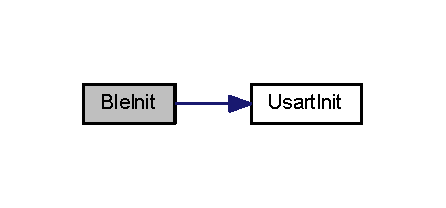
\includegraphics[width=214pt]{group___b_l_e_gad65e0136086cff966fcbd14a10a8a313_cgraph}
\end{center}
\end{figure}




\-Here is the caller graph for this function\-:\nopagebreak
\begin{figure}[H]
\begin{center}
\leavevmode
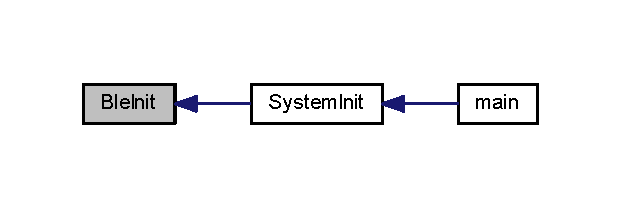
\includegraphics[width=298pt]{group___b_l_e_gad65e0136086cff966fcbd14a10a8a313_icgraph}
\end{center}
\end{figure}


\hypertarget{group___b_l_e_ga0c4cf6eee7dc11b12abf30972e242b05}{\index{\-Bsp\-Ble\-: B\-S\-P Group@{\-Bsp\-Ble\-: B\-S\-P Group}!\-Ble\-Send@{\-Ble\-Send}}
\index{\-Ble\-Send@{\-Ble\-Send}!BspBle: BSP Group@{\-Bsp\-Ble\-: B\-S\-P Group}}
\subsubsection[{\-Ble\-Send}]{\setlength{\rightskip}{0pt plus 5cm}void {\bf \-Ble\-Send} (
\begin{DoxyParamCaption}
\item[{void}]{}
\end{DoxyParamCaption}
)}}\label{group___b_l_e_ga0c4cf6eee7dc11b12abf30972e242b05}


蓝牙发送状态机 


\begin{DoxyParams}{\-Parameters}
{\em 参数名} & 参数说明 \\
\hline
{\em 无} & \\
\hline
\end{DoxyParams}

\begin{DoxyRetVals}{\-Return values}
{\em 无} & \\
\hline
\end{DoxyRetVals}
\begin{DoxyParagraph}{使用全局变量 }

\end{DoxyParagraph}
\begin{DoxyNote}{\-Note}
● 执行时间\-: \par
 ● 调用周期\-: 1ms \par
 ● 可否打断\-: 可以 \par

\end{DoxyNote}
\begin{DoxyParagraph}{注意\-:}
● 由于该蓝牙模块在发送数据前需先将发送引脚拉低至少500us,发送完成后需至少等待200us再将发送引脚拉高,故采用此状态机取代延时等待 \par
 
\end{DoxyParagraph}


\-Here is the call graph for this function\-:\nopagebreak
\begin{figure}[H]
\begin{center}
\leavevmode
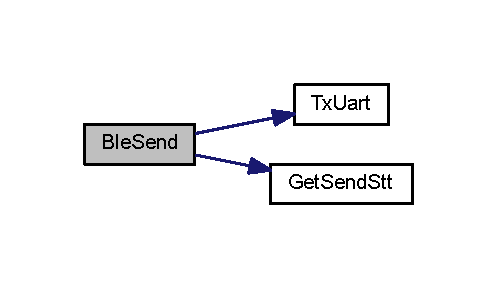
\includegraphics[width=238pt]{group___b_l_e_ga0c4cf6eee7dc11b12abf30972e242b05_cgraph}
\end{center}
\end{figure}


\hypertarget{group___b_l_e_ga738473a5b43f6c92b80ce1d3d6f77ed9}{\index{\-Bsp\-Ble\-: B\-S\-P Group@{\-Bsp\-Ble\-: B\-S\-P Group}!\-E\-X\-T\-I15\-\_\-10\-\_\-\-I\-R\-Q\-Handler@{\-E\-X\-T\-I15\-\_\-10\-\_\-\-I\-R\-Q\-Handler}}
\index{\-E\-X\-T\-I15\-\_\-10\-\_\-\-I\-R\-Q\-Handler@{\-E\-X\-T\-I15\-\_\-10\-\_\-\-I\-R\-Q\-Handler}!BspBle: BSP Group@{\-Bsp\-Ble\-: B\-S\-P Group}}
\subsubsection[{\-E\-X\-T\-I15\-\_\-10\-\_\-\-I\-R\-Q\-Handler}]{\setlength{\rightskip}{0pt plus 5cm}void {\bf \-E\-X\-T\-I15\-\_\-10\-\_\-\-I\-R\-Q\-Handler} (
\begin{DoxyParamCaption}
\item[{void}]{}
\end{DoxyParamCaption}
)}}\label{group___b_l_e_ga738473a5b43f6c92b80ce1d3d6f77ed9}


10$\sim$15通道外部中断处理函数 


\begin{DoxyParams}{\-Parameters}
{\em 参数名} & 参数说明 \\
\hline
{\em 无} & \\
\hline
\end{DoxyParams}

\begin{DoxyRetVals}{\-Return values}
{\em 无} & \\
\hline
\end{DoxyRetVals}
\begin{DoxyParagraph}{使用全局变量 }

\end{DoxyParagraph}
\begin{DoxyNote}{\-Note}
● 执行时间\-: \par
 ● 调用周期\-: 触发调用 \par
 ● 可否打断\-: 不可以 \par

\end{DoxyNote}
\begin{DoxyParagraph}{注意\-:}
● 12通道用于下键中断,仅在睡眠前开启,用于按键将系统从睡眠中唤醒 \par
 ● 10通道用于蓝牙连接状态变化断 \par
 
\end{DoxyParagraph}
\hypertarget{group___b_l_e_ga3fc122f9e39ecffe66a227b87d6051eb}{\index{\-Bsp\-Ble\-: B\-S\-P Group@{\-Bsp\-Ble\-: B\-S\-P Group}!\-Push\-Send\-Buf@{\-Push\-Send\-Buf}}
\index{\-Push\-Send\-Buf@{\-Push\-Send\-Buf}!BspBle: BSP Group@{\-Bsp\-Ble\-: B\-S\-P Group}}
\subsubsection[{\-Push\-Send\-Buf}]{\setlength{\rightskip}{0pt plus 5cm}{\bf u8} {\bf \-Push\-Send\-Buf} (
\begin{DoxyParamCaption}
\item[{{\bf u8} $\ast$}]{data, }
\item[{{\bf u8}}]{len}
\end{DoxyParamCaption}
)}}\label{group___b_l_e_ga3fc122f9e39ecffe66a227b87d6051eb}


将需要发送的数据写入缓冲区 


\begin{DoxyParams}[1]{\-Parameters}
 & {\em 参数名} & 参数说明 \\
\hline
\mbox{\tt in}  & {\em $\ast$data} & 发送的数据指针 \\
\hline
\mbox{\tt in}  & {\em len} & 发送的数据长度 \\
\hline
\end{DoxyParams}

\begin{DoxyRetVals}{\-Return values}
{\em 无} & \\
\hline
\end{DoxyRetVals}
\begin{DoxyParagraph}{使用全局变量}
无 \par
 
\end{DoxyParagraph}
\begin{DoxyNote}{\-Note}
● 执行时间\-: \par
 ● 调用周期\-: 触发调用 \par
 ● 可否打断\-: 可以 \par

\end{DoxyNote}
\begin{DoxyParagraph}{注意\-:}
● 无 
\end{DoxyParagraph}

\hypertarget{group___k_e_y}{\section{\-Bsp\-Key\-: \-B\-S\-P \-Group}
\label{group___k_e_y}\index{\-Bsp\-Key\-: B\-S\-P Group@{\-Bsp\-Key\-: B\-S\-P Group}}
}
\subsection*{\-Data \-Structures}
\begin{DoxyCompactItemize}
\item 
union \hyperlink{union_u_n___key_stt}{\-U\-N\-\_\-\-Key\-Stt}
\begin{DoxyCompactList}\small\item\em 按键状态联合体 \end{DoxyCompactList}\item 
struct \hyperlink{struct_s_t_r___key}{\-S\-T\-R\-\_\-\-Key}
\begin{DoxyCompactList}\small\item\em 按键状态结构体 \end{DoxyCompactList}\end{DoxyCompactItemize}
\subsection*{\-Defines}
\begin{DoxyCompactItemize}
\item 
\#define \hyperlink{group___k_e_y_ga38599380071fb33212aa3fd543bae31b}{\-K\-E\-Y\-\_\-\-D\-N\-\_\-\-F\-L\-T}~100
\begin{DoxyCompactList}\small\item\em 按键按下滤波次数,每次1ms \end{DoxyCompactList}\item 
\#define \hyperlink{group___k_e_y_gae1e078d7683b2244f76e0cec7526899d}{\-K\-E\-Y\-\_\-\-U\-P\-\_\-\-F\-L\-T}~50
\begin{DoxyCompactList}\small\item\em 按键弹起滤波次数,每次1ms \end{DoxyCompactList}\item 
\#define \hyperlink{group___k_e_y_ga69ed1676c835686c30dbdc821661954b}{\-K\-E\-Y\-\_\-\-L\-O\-N\-G}~900
\begin{DoxyCompactList}\small\item\em 按键长按滤波次数,每次1ms \end{DoxyCompactList}\item 
\hypertarget{group___k_e_y_gab3cfff9440c221292481854752c3bc13}{\#define \hyperlink{group___k_e_y_gab3cfff9440c221292481854752c3bc13}{\-K\-E\-Y\-\_\-\-N\-V\-I\-C\-\_\-\-P\-R\-I\-O}~15;}\label{group___k_e_y_gab3cfff9440c221292481854752c3bc13}

\begin{DoxyCompactList}\small\item\em 按键中断优先级 \end{DoxyCompactList}\end{DoxyCompactItemize}
\subsection*{\-Functions}
\begin{DoxyCompactItemize}
\item 
void \hyperlink{group___k_e_y_gae487e92ffd4829b2f098684a5e9b6738}{\-Key\-Init} (void)
\begin{DoxyCompactList}\small\item\em 按键初始化函数 \end{DoxyCompactList}\item 
void \hyperlink{group___k_e_y_gaee3a5acfe28e98d56137a5381fe731d2}{\-Set\-Key\-Int} (\hyperlink{group___b_s_p_gaed742c436da53c1080638ce6ef7d13de}{u8} new\-Stt)
\begin{DoxyCompactList}\small\item\em 设置按键中断函数 \end{DoxyCompactList}\item 
void \hyperlink{group___k_e_y_ga3270aa3bb293f0e41c049552f49b3f5c}{\-Key\-Scan} (\hyperlink{struct_s_t_r___key}{\-S\-T\-R\-\_\-\-Key} $\ast$key)
\begin{DoxyCompactList}\small\item\em 按键扫描函数 \end{DoxyCompactList}\item 
void \hyperlink{group___k_e_y_ga49cfdd46eb8d0ef3e1987514aa9343dc}{\-E\-X\-T\-I1\-\_\-\-I\-R\-Q\-Handler} (void)
\begin{DoxyCompactList}\small\item\em 1通道外部中断处理函数 \end{DoxyCompactList}\item 
void \hyperlink{group___k_e_y_ga7b2096b8b2643286dc3a7e5110e5ae85}{\-E\-X\-T\-I9\-\_\-5\-\_\-\-I\-R\-Q\-Handler} (void)
\begin{DoxyCompactList}\small\item\em 5$\sim$9通道外部中断处理函数 \end{DoxyCompactList}\end{DoxyCompactItemize}
\subsection*{\-Variables}
\begin{DoxyCompactItemize}
\item 
\hypertarget{group___k_e_y_ga16e6f341748e390fbbc27d40a89053a1}{\hyperlink{struct_s_t_r___key}{\-S\-T\-R\-\_\-\-Key} \hyperlink{group___k_e_y_ga16e6f341748e390fbbc27d40a89053a1}{\-Key\-Stt}}\label{group___k_e_y_ga16e6f341748e390fbbc27d40a89053a1}

\begin{DoxyCompactList}\small\item\em 按键状态结构体 \end{DoxyCompactList}\item 
\hypertarget{group___k_e_y_ga16e6f341748e390fbbc27d40a89053a1}{\hyperlink{struct_s_t_r___key}{\-S\-T\-R\-\_\-\-Key} \hyperlink{group___k_e_y_ga16e6f341748e390fbbc27d40a89053a1}{\-Key\-Stt}}\label{group___k_e_y_ga16e6f341748e390fbbc27d40a89053a1}

\begin{DoxyCompactList}\small\item\em 按键状态结构体 \end{DoxyCompactList}\end{DoxyCompactItemize}


\subsection{\-Define \-Documentation}
\hypertarget{group___k_e_y_ga38599380071fb33212aa3fd543bae31b}{\index{\-Bsp\-Key\-: B\-S\-P Group@{\-Bsp\-Key\-: B\-S\-P Group}!\-K\-E\-Y\-\_\-\-D\-N\-\_\-\-F\-L\-T@{\-K\-E\-Y\-\_\-\-D\-N\-\_\-\-F\-L\-T}}
\index{\-K\-E\-Y\-\_\-\-D\-N\-\_\-\-F\-L\-T@{\-K\-E\-Y\-\_\-\-D\-N\-\_\-\-F\-L\-T}!BspKey: BSP Group@{\-Bsp\-Key\-: B\-S\-P Group}}
\subsubsection[{\-K\-E\-Y\-\_\-\-D\-N\-\_\-\-F\-L\-T}]{\setlength{\rightskip}{0pt plus 5cm}\#define {\bf \-K\-E\-Y\-\_\-\-D\-N\-\_\-\-F\-L\-T}~100}}\label{group___k_e_y_ga38599380071fb33212aa3fd543bae31b}


按键按下滤波次数,每次1ms 

相当于 100ms \hypertarget{group___k_e_y_ga69ed1676c835686c30dbdc821661954b}{\index{\-Bsp\-Key\-: B\-S\-P Group@{\-Bsp\-Key\-: B\-S\-P Group}!\-K\-E\-Y\-\_\-\-L\-O\-N\-G@{\-K\-E\-Y\-\_\-\-L\-O\-N\-G}}
\index{\-K\-E\-Y\-\_\-\-L\-O\-N\-G@{\-K\-E\-Y\-\_\-\-L\-O\-N\-G}!BspKey: BSP Group@{\-Bsp\-Key\-: B\-S\-P Group}}
\subsubsection[{\-K\-E\-Y\-\_\-\-L\-O\-N\-G}]{\setlength{\rightskip}{0pt plus 5cm}\#define {\bf \-K\-E\-Y\-\_\-\-L\-O\-N\-G}~900}}\label{group___k_e_y_ga69ed1676c835686c30dbdc821661954b}


按键长按滤波次数,每次1ms 

相当于 900ms \hypertarget{group___k_e_y_gae1e078d7683b2244f76e0cec7526899d}{\index{\-Bsp\-Key\-: B\-S\-P Group@{\-Bsp\-Key\-: B\-S\-P Group}!\-K\-E\-Y\-\_\-\-U\-P\-\_\-\-F\-L\-T@{\-K\-E\-Y\-\_\-\-U\-P\-\_\-\-F\-L\-T}}
\index{\-K\-E\-Y\-\_\-\-U\-P\-\_\-\-F\-L\-T@{\-K\-E\-Y\-\_\-\-U\-P\-\_\-\-F\-L\-T}!BspKey: BSP Group@{\-Bsp\-Key\-: B\-S\-P Group}}
\subsubsection[{\-K\-E\-Y\-\_\-\-U\-P\-\_\-\-F\-L\-T}]{\setlength{\rightskip}{0pt plus 5cm}\#define {\bf \-K\-E\-Y\-\_\-\-U\-P\-\_\-\-F\-L\-T}~50}}\label{group___k_e_y_gae1e078d7683b2244f76e0cec7526899d}


按键弹起滤波次数,每次1ms 

相当于 50ms 

\subsection{\-Function \-Documentation}
\hypertarget{group___k_e_y_ga49cfdd46eb8d0ef3e1987514aa9343dc}{\index{\-Bsp\-Key\-: B\-S\-P Group@{\-Bsp\-Key\-: B\-S\-P Group}!\-E\-X\-T\-I1\-\_\-\-I\-R\-Q\-Handler@{\-E\-X\-T\-I1\-\_\-\-I\-R\-Q\-Handler}}
\index{\-E\-X\-T\-I1\-\_\-\-I\-R\-Q\-Handler@{\-E\-X\-T\-I1\-\_\-\-I\-R\-Q\-Handler}!BspKey: BSP Group@{\-Bsp\-Key\-: B\-S\-P Group}}
\subsubsection[{\-E\-X\-T\-I1\-\_\-\-I\-R\-Q\-Handler}]{\setlength{\rightskip}{0pt plus 5cm}void {\bf \-E\-X\-T\-I1\-\_\-\-I\-R\-Q\-Handler} (
\begin{DoxyParamCaption}
\item[{void}]{}
\end{DoxyParamCaption}
)}}\label{group___k_e_y_ga49cfdd46eb8d0ef3e1987514aa9343dc}


1通道外部中断处理函数 


\begin{DoxyParams}{\-Parameters}
{\em 参数名} & 参数说明 \\
\hline
{\em 无} & \\
\hline
\end{DoxyParams}

\begin{DoxyRetVals}{\-Return values}
{\em 无} & \\
\hline
\end{DoxyRetVals}
\begin{DoxyParagraph}{使用全局变量 }

\end{DoxyParagraph}
\begin{DoxyNote}{\-Note}
● 执行时间\-: \par
 ● 调用周期\-: 触发调用 \par
 ● 可否打断\-: 不可以 \par

\end{DoxyNote}
\begin{DoxyParagraph}{注意\-:}
● 1通道用于右键中断,仅在睡眠前开启,用于按键将系统从睡眠中唤醒 \par
 
\end{DoxyParagraph}
\hypertarget{group___k_e_y_ga7b2096b8b2643286dc3a7e5110e5ae85}{\index{\-Bsp\-Key\-: B\-S\-P Group@{\-Bsp\-Key\-: B\-S\-P Group}!\-E\-X\-T\-I9\-\_\-5\-\_\-\-I\-R\-Q\-Handler@{\-E\-X\-T\-I9\-\_\-5\-\_\-\-I\-R\-Q\-Handler}}
\index{\-E\-X\-T\-I9\-\_\-5\-\_\-\-I\-R\-Q\-Handler@{\-E\-X\-T\-I9\-\_\-5\-\_\-\-I\-R\-Q\-Handler}!BspKey: BSP Group@{\-Bsp\-Key\-: B\-S\-P Group}}
\subsubsection[{\-E\-X\-T\-I9\-\_\-5\-\_\-\-I\-R\-Q\-Handler}]{\setlength{\rightskip}{0pt plus 5cm}void {\bf \-E\-X\-T\-I9\-\_\-5\-\_\-\-I\-R\-Q\-Handler} (
\begin{DoxyParamCaption}
\item[{void}]{}
\end{DoxyParamCaption}
)}}\label{group___k_e_y_ga7b2096b8b2643286dc3a7e5110e5ae85}


5$\sim$9通道外部中断处理函数 


\begin{DoxyParams}{\-Parameters}
{\em 参数名} & 参数说明 \\
\hline
{\em 无} & \\
\hline
\end{DoxyParams}

\begin{DoxyRetVals}{\-Return values}
{\em 无} & \\
\hline
\end{DoxyRetVals}
\begin{DoxyParagraph}{使用全局变量 }

\end{DoxyParagraph}
\begin{DoxyNote}{\-Note}
● 执行时间\-: \par
 ● 调用周期\-: 触发调用 \par
 ● 可否打断\-: 不可以 \par

\end{DoxyNote}
\begin{DoxyParagraph}{注意\-:}
● 8通道用于左键中断,仅在睡眠前开启,用于按键将系统从睡眠中唤醒 \par
 
\end{DoxyParagraph}
\hypertarget{group___k_e_y_gae487e92ffd4829b2f098684a5e9b6738}{\index{\-Bsp\-Key\-: B\-S\-P Group@{\-Bsp\-Key\-: B\-S\-P Group}!\-Key\-Init@{\-Key\-Init}}
\index{\-Key\-Init@{\-Key\-Init}!BspKey: BSP Group@{\-Bsp\-Key\-: B\-S\-P Group}}
\subsubsection[{\-Key\-Init}]{\setlength{\rightskip}{0pt plus 5cm}void {\bf \-Key\-Init} (
\begin{DoxyParamCaption}
\item[{void}]{}
\end{DoxyParamCaption}
)}}\label{group___k_e_y_gae487e92ffd4829b2f098684a5e9b6738}


按键初始化函数 


\begin{DoxyParams}{\-Parameters}
{\em 参数名} & 参数说明 \\
\hline
{\em 无} & \\
\hline
\end{DoxyParams}

\begin{DoxyRetVals}{\-Return values}
{\em 无} & \\
\hline
\end{DoxyRetVals}
\begin{DoxyParagraph}{使用全局变量 }

\end{DoxyParagraph}
\begin{DoxyNote}{\-Note}
● 执行时间\-: \par
 ● 调用周期\-: 触发调用, 初始化时调用 \par
 ● 可否打断\-: 可以 \par

\end{DoxyNote}
\begin{DoxyParagraph}{注意\-:}
● 无 \par
 
\end{DoxyParagraph}


\-Here is the caller graph for this function\-:\nopagebreak
\begin{figure}[H]
\begin{center}
\leavevmode
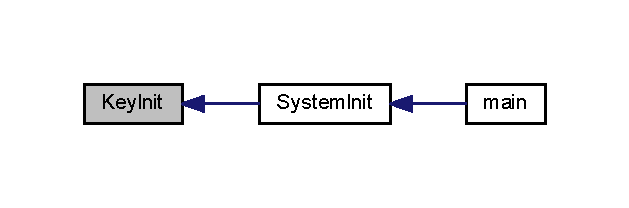
\includegraphics[width=302pt]{group___k_e_y_gae487e92ffd4829b2f098684a5e9b6738_icgraph}
\end{center}
\end{figure}


\hypertarget{group___k_e_y_ga3270aa3bb293f0e41c049552f49b3f5c}{\index{\-Bsp\-Key\-: B\-S\-P Group@{\-Bsp\-Key\-: B\-S\-P Group}!\-Key\-Scan@{\-Key\-Scan}}
\index{\-Key\-Scan@{\-Key\-Scan}!BspKey: BSP Group@{\-Bsp\-Key\-: B\-S\-P Group}}
\subsubsection[{\-Key\-Scan}]{\setlength{\rightskip}{0pt plus 5cm}void {\bf \-Key\-Scan} (
\begin{DoxyParamCaption}
\item[{{\bf \-S\-T\-R\-\_\-\-Key} $\ast$}]{key}
\end{DoxyParamCaption}
)}}\label{group___k_e_y_ga3270aa3bb293f0e41c049552f49b3f5c}


按键扫描函数 


\begin{DoxyParams}[1]{\-Parameters}
 & {\em 参数名} & 参数说明 \\
\hline
\mbox{\tt in}  & {\em key} & 按键结构体指针 \\
\hline
\end{DoxyParams}

\begin{DoxyRetVals}{\-Return values}
{\em 无} & \\
\hline
\end{DoxyRetVals}
\begin{DoxyParagraph}{使用全局变量 }

\end{DoxyParagraph}
\begin{DoxyNote}{\-Note}
● 执行时间\-: \par
 ● 调用周期\-: 1ms \par
 ● 可否打断\-: 可以 \par

\end{DoxyNote}
\begin{DoxyParagraph}{注意\-:}
● 无 \par
 
\end{DoxyParagraph}
\hypertarget{group___k_e_y_gaee3a5acfe28e98d56137a5381fe731d2}{\index{\-Bsp\-Key\-: B\-S\-P Group@{\-Bsp\-Key\-: B\-S\-P Group}!\-Set\-Key\-Int@{\-Set\-Key\-Int}}
\index{\-Set\-Key\-Int@{\-Set\-Key\-Int}!BspKey: BSP Group@{\-Bsp\-Key\-: B\-S\-P Group}}
\subsubsection[{\-Set\-Key\-Int}]{\setlength{\rightskip}{0pt plus 5cm}void {\bf \-Set\-Key\-Int} (
\begin{DoxyParamCaption}
\item[{{\bf u8}}]{new\-Stt}
\end{DoxyParamCaption}
)}}\label{group___k_e_y_gaee3a5acfe28e98d56137a5381fe731d2}


设置按键中断函数 


\begin{DoxyParams}[1]{\-Parameters}
 & {\em 参数名} & 参数说明 \\
\hline
\mbox{\tt in}  & {\em new\-Stt} & 需要设置的中断状态 \\
\hline
\end{DoxyParams}

\begin{DoxyRetVals}{\-Return values}
{\em 无} & \\
\hline
\end{DoxyRetVals}
\begin{DoxyParagraph}{使用全局变量 }

\end{DoxyParagraph}
\begin{DoxyNote}{\-Note}
● 执行时间\-: \par
 ● 调用周期\-: 触发调用 \par
 ● 可否打断\-: 可以 \par

\end{DoxyNote}
\begin{DoxyParagraph}{注意\-:}
● 无 \par
 
\end{DoxyParagraph}

\hypertarget{group___l_e_d}{\section{\-Bsp\-Led\-: \-B\-S\-P \-Group}
\label{group___l_e_d}\index{\-Bsp\-Led\-: B\-S\-P Group@{\-Bsp\-Led\-: B\-S\-P Group}}
}
\subsection*{\-Data \-Structures}
\begin{DoxyCompactItemize}
\item 
struct \hyperlink{struct_s_t_r___light}{\-S\-T\-R\-\_\-\-Light}
\begin{DoxyCompactList}\small\item\em \-L\-E\-D照明模式结构体 \end{DoxyCompactList}\item 
struct \hyperlink{struct_s_t_r___color}{\-S\-T\-R\-\_\-\-Color}
\begin{DoxyCompactList}\small\item\em \-L\-E\-D彩灯模式结构体 \end{DoxyCompactList}\item 
struct \hyperlink{struct_s_t_r___led}{\-S\-T\-R\-\_\-\-Led}
\begin{DoxyCompactList}\small\item\em \-L\-E\-D结构体 \end{DoxyCompactList}\end{DoxyCompactItemize}
\subsection*{\-Defines}
\begin{DoxyCompactItemize}
\item 
\hypertarget{group___l_e_d_ga2bb5240f10b359f924e69d10d1accd07}{\#define \hyperlink{group___l_e_d_ga2bb5240f10b359f924e69d10d1accd07}{\-L\-E\-D\-\_\-\-L\-I\-G\-H\-T}~0}\label{group___l_e_d_ga2bb5240f10b359f924e69d10d1accd07}

\begin{DoxyCompactList}\small\item\em 照明模式 \end{DoxyCompactList}\item 
\hypertarget{group___l_e_d_ga1a390ed4322d9bfdba9add7bba7a0c8d}{\#define \hyperlink{group___l_e_d_ga1a390ed4322d9bfdba9add7bba7a0c8d}{\-L\-E\-D\-\_\-\-C\-O\-L\-O\-R}~1}\label{group___l_e_d_ga1a390ed4322d9bfdba9add7bba7a0c8d}

\begin{DoxyCompactList}\small\item\em 彩灯模式 \end{DoxyCompactList}\item 
\hypertarget{group___l_e_d_ga9be8a14dcc537a96262bfbf707c8c7f2}{\#define \hyperlink{group___l_e_d_ga9be8a14dcc537a96262bfbf707c8c7f2}{\-L\-E\-D\-\_\-\-L\-O\-P\-W\-R}~2}\label{group___l_e_d_ga9be8a14dcc537a96262bfbf707c8c7f2}

\begin{DoxyCompactList}\small\item\em 低电量警告 \end{DoxyCompactList}\end{DoxyCompactItemize}
\subsection*{\-Functions}
\begin{DoxyCompactItemize}
\item 
void \hyperlink{group___l_e_d_ga1d5b4eaf7f01ae9557ba620158ebdfd9}{\-Led\-Init} (void)
\begin{DoxyCompactList}\small\item\em \-Led初始化函数 \end{DoxyCompactList}\item 
void \hyperlink{group___l_e_d_gae8b99ece48c700224bfdc62518a1a0ec}{\-Set\-Light} (\hyperlink{group___b_s_p_ga9e6c91d77e24643b888dbd1a1a590054}{u16} light, \hyperlink{group___b_s_p_ga10e94b422ef0c20dcdec20d31a1f5049}{u32} delay)
\begin{DoxyCompactList}\small\item\em 设置照明模式函数 \end{DoxyCompactList}\item 
void \hyperlink{group___l_e_d_gacc86e7dba3879210d60ccc467ae5e228}{\-Set\-Color} (\hyperlink{group___b_s_p_ga9e6c91d77e24643b888dbd1a1a590054}{u16} r, \hyperlink{group___b_s_p_ga9e6c91d77e24643b888dbd1a1a590054}{u16} g, \hyperlink{group___b_s_p_ga9e6c91d77e24643b888dbd1a1a590054}{u16} b, \hyperlink{group___b_s_p_gaed742c436da53c1080638ce6ef7d13de}{u8} breath)
\begin{DoxyCompactList}\small\item\em 设置照明模式函数 \end{DoxyCompactList}\item 
void \hyperlink{group___l_e_d_ga5e50d2839709fdab79e8efb08d9d69cd}{\-Led\-Upd\-Stt} (\hyperlink{struct_s_t_r___led}{\-S\-T\-R\-\_\-\-Led} $\ast$led)
\begin{DoxyCompactList}\small\item\em \-L\-E\-D状态更新函数 \end{DoxyCompactList}\end{DoxyCompactItemize}
\subsection*{\-Variables}
\begin{DoxyCompactItemize}
\item 
\hypertarget{group___l_e_d_ga4f3cfc9a345d42364106b78ccd152b93}{\hyperlink{struct_s_t_r___led}{\-S\-T\-R\-\_\-\-Led} \hyperlink{group___l_e_d_ga4f3cfc9a345d42364106b78ccd152b93}{\-Led} = \{0,\}}\label{group___l_e_d_ga4f3cfc9a345d42364106b78ccd152b93}

\begin{DoxyCompactList}\small\item\em \-L\-E\-D结构体 \end{DoxyCompactList}\item 
\hypertarget{group___l_e_d_ga4f3cfc9a345d42364106b78ccd152b93}{\hyperlink{struct_s_t_r___led}{\-S\-T\-R\-\_\-\-Led} \hyperlink{group___l_e_d_ga4f3cfc9a345d42364106b78ccd152b93}{\-Led}}\label{group___l_e_d_ga4f3cfc9a345d42364106b78ccd152b93}

\begin{DoxyCompactList}\small\item\em \-L\-E\-D结构体 \end{DoxyCompactList}\end{DoxyCompactItemize}


\subsection{\-Function \-Documentation}
\hypertarget{group___l_e_d_ga1d5b4eaf7f01ae9557ba620158ebdfd9}{\index{\-Bsp\-Led\-: B\-S\-P Group@{\-Bsp\-Led\-: B\-S\-P Group}!\-Led\-Init@{\-Led\-Init}}
\index{\-Led\-Init@{\-Led\-Init}!BspLed: BSP Group@{\-Bsp\-Led\-: B\-S\-P Group}}
\subsubsection[{\-Led\-Init}]{\setlength{\rightskip}{0pt plus 5cm}void {\bf \-Led\-Init} (
\begin{DoxyParamCaption}
\item[{void}]{}
\end{DoxyParamCaption}
)}}\label{group___l_e_d_ga1d5b4eaf7f01ae9557ba620158ebdfd9}


\-Led初始化函数 


\begin{DoxyParams}{\-Parameters}
{\em 参数名} & 参数说明 \\
\hline
{\em 无} & \\
\hline
\end{DoxyParams}

\begin{DoxyRetVals}{\-Return values}
{\em 无} & \\
\hline
\end{DoxyRetVals}
\begin{DoxyParagraph}{使用全局变量 }

\end{DoxyParagraph}
\begin{DoxyNote}{\-Note}
● 执行时间\-: \par
 ● 调用周期\-: 触发调用, 初始化时调用 \par
 ● 可否打断\-: 可以 \par

\end{DoxyNote}
\begin{DoxyParagraph}{注意\-:}
● 无 \par
 
\end{DoxyParagraph}


\-Here is the call graph for this function\-:\nopagebreak
\begin{figure}[H]
\begin{center}
\leavevmode
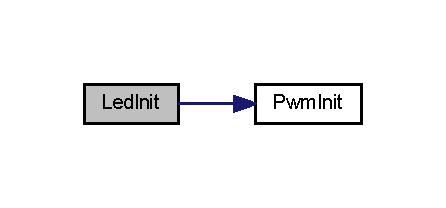
\includegraphics[width=214pt]{group___l_e_d_ga1d5b4eaf7f01ae9557ba620158ebdfd9_cgraph}
\end{center}
\end{figure}




\-Here is the caller graph for this function\-:\nopagebreak
\begin{figure}[H]
\begin{center}
\leavevmode
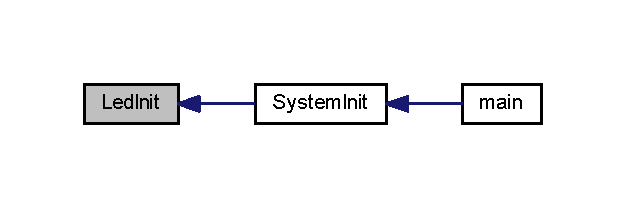
\includegraphics[width=300pt]{group___l_e_d_ga1d5b4eaf7f01ae9557ba620158ebdfd9_icgraph}
\end{center}
\end{figure}


\hypertarget{group___l_e_d_ga5e50d2839709fdab79e8efb08d9d69cd}{\index{\-Bsp\-Led\-: B\-S\-P Group@{\-Bsp\-Led\-: B\-S\-P Group}!\-Led\-Upd\-Stt@{\-Led\-Upd\-Stt}}
\index{\-Led\-Upd\-Stt@{\-Led\-Upd\-Stt}!BspLed: BSP Group@{\-Bsp\-Led\-: B\-S\-P Group}}
\subsubsection[{\-Led\-Upd\-Stt}]{\setlength{\rightskip}{0pt plus 5cm}void {\bf \-Led\-Upd\-Stt} (
\begin{DoxyParamCaption}
\item[{{\bf \-S\-T\-R\-\_\-\-Led} $\ast$}]{led}
\end{DoxyParamCaption}
)}}\label{group___l_e_d_ga5e50d2839709fdab79e8efb08d9d69cd}


\-L\-E\-D状态更新函数 


\begin{DoxyParams}[1]{\-Parameters}
 & {\em 参数名} & 参数说明 \\
\hline
\mbox{\tt in}  & {\em led} & \-L\-E\-D结构体指针 \\
\hline
\end{DoxyParams}

\begin{DoxyRetVals}{\-Return values}
{\em 无} & \\
\hline
\end{DoxyRetVals}
\begin{DoxyParagraph}{使用全局变量 }

\end{DoxyParagraph}
\begin{DoxyNote}{\-Note}
● 执行时间\-: \par
 ● 调用周期\-: 20ms \par
 ● 可否打断\-: 可以 \par

\end{DoxyNote}
\begin{DoxyParagraph}{注意\-:}
● 无 \par
 
\end{DoxyParagraph}


\-Here is the call graph for this function\-:\nopagebreak
\begin{figure}[H]
\begin{center}
\leavevmode
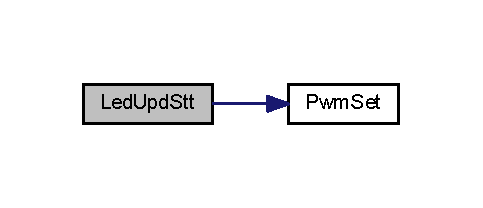
\includegraphics[width=232pt]{group___l_e_d_ga5e50d2839709fdab79e8efb08d9d69cd_cgraph}
\end{center}
\end{figure}


\hypertarget{group___l_e_d_gacc86e7dba3879210d60ccc467ae5e228}{\index{\-Bsp\-Led\-: B\-S\-P Group@{\-Bsp\-Led\-: B\-S\-P Group}!\-Set\-Color@{\-Set\-Color}}
\index{\-Set\-Color@{\-Set\-Color}!BspLed: BSP Group@{\-Bsp\-Led\-: B\-S\-P Group}}
\subsubsection[{\-Set\-Color}]{\setlength{\rightskip}{0pt plus 5cm}void {\bf \-Set\-Color} (
\begin{DoxyParamCaption}
\item[{{\bf u16}}]{r, }
\item[{{\bf u16}}]{g, }
\item[{{\bf u16}}]{b, }
\item[{{\bf u8}}]{breath}
\end{DoxyParamCaption}
)}}\label{group___l_e_d_gacc86e7dba3879210d60ccc467ae5e228}


设置照明模式函数 


\begin{DoxyParams}[1]{\-Parameters}
 & {\em 参数名} & 参数说明 \\
\hline
\mbox{\tt in}  & {\em r} & 红光亮度 \\
\hline
\mbox{\tt in}  & {\em g} & 绿光亮度 \\
\hline
\mbox{\tt in}  & {\em b} & 蓝光亮度 \\
\hline
\mbox{\tt in}  & {\em breath} & 呼吸灯使能 \\
\hline
\end{DoxyParams}

\begin{DoxyRetVals}{\-Return values}
{\em 无} & \\
\hline
\end{DoxyRetVals}
\begin{DoxyParagraph}{使用全局变量 }

\end{DoxyParagraph}
\begin{DoxyNote}{\-Note}
● 执行时间\-: \par
 ● 调用周期\-: 500us \par
 ● 可否打断\-: 可以 \par

\end{DoxyNote}
\begin{DoxyParagraph}{注意\-:}
● 无 \par
 
\end{DoxyParagraph}
\hypertarget{group___l_e_d_gae8b99ece48c700224bfdc62518a1a0ec}{\index{\-Bsp\-Led\-: B\-S\-P Group@{\-Bsp\-Led\-: B\-S\-P Group}!\-Set\-Light@{\-Set\-Light}}
\index{\-Set\-Light@{\-Set\-Light}!BspLed: BSP Group@{\-Bsp\-Led\-: B\-S\-P Group}}
\subsubsection[{\-Set\-Light}]{\setlength{\rightskip}{0pt plus 5cm}void {\bf \-Set\-Light} (
\begin{DoxyParamCaption}
\item[{{\bf u16}}]{light, }
\item[{{\bf u32}}]{delay}
\end{DoxyParamCaption}
)}}\label{group___l_e_d_gae8b99ece48c700224bfdc62518a1a0ec}


设置照明模式函数 


\begin{DoxyParams}[1]{\-Parameters}
 & {\em 参数名} & 参数说明 \\
\hline
\mbox{\tt in}  & {\em light} & 亮度 \\
\hline
\mbox{\tt in}  & {\em delay} & 延时, 单位\-: 秒 \\
\hline
\end{DoxyParams}

\begin{DoxyRetVals}{\-Return values}
{\em 无} & \\
\hline
\end{DoxyRetVals}
\begin{DoxyParagraph}{使用全局变量 }

\end{DoxyParagraph}
\begin{DoxyNote}{\-Note}
● 执行时间\-: \par
 ● 调用周期\-: 500us \par
 ● 可否打断\-: 可以 \par

\end{DoxyNote}
\begin{DoxyParagraph}{注意\-:}
● 无 \par
 
\end{DoxyParagraph}

\hypertarget{group___o_l_e_d}{\section{\-Bsp\-Oled\-: \-B\-S\-P \-Group}
\label{group___o_l_e_d}\index{\-Bsp\-Oled\-: B\-S\-P Group@{\-Bsp\-Oled\-: B\-S\-P Group}}
}
\subsection*{\-Defines}
\begin{DoxyCompactItemize}
\item 
\#define \hyperlink{group___o_l_e_d_ga7d467c1d283fdfa1f2081ba1e0d01b6e}{\-P\-A\-G\-E\-\_\-\-S\-I\-Z\-E}~1024
\begin{DoxyCompactList}\small\item\em 如果采用3线\-S\-P\-I, 每个字节除了8bit数据, 还需要发1bit的\-D/\-C信号; 而stm32f10x不支持9bit硬件\-S\-P\-I, 故手动将8bit扩充为9bit, 缓冲区是原来的 9/8 倍 \end{DoxyCompactList}\item 
\hypertarget{group___o_l_e_d_gaba889888734a8b272a51d444d70ad2fa}{\#define \hyperlink{group___o_l_e_d_gaba889888734a8b272a51d444d70ad2fa}{\-L\-I\-N\-E\-\_\-\-S\-I\-Z\-E}~128}\label{group___o_l_e_d_gaba889888734a8b272a51d444d70ad2fa}

\begin{DoxyCompactList}\small\item\em 1024 / 8 = 128; \end{DoxyCompactList}\item 
\#define \hyperlink{group___o_l_e_d_ga4c0102b3d63c7bd2d59a424ca3815ad1}{\-L\-I\-N\-E1}~0
\begin{DoxyCompactList}\small\item\em 每一行的第一个列在缓冲区中的偏移 \end{DoxyCompactList}\item 
\hypertarget{group___o_l_e_d_ga259e96afd23afb9e2fd9e97d5e07193c}{\#define \hyperlink{group___o_l_e_d_ga259e96afd23afb9e2fd9e97d5e07193c}{\-L\-I\-N\-E2}~128}\label{group___o_l_e_d_ga259e96afd23afb9e2fd9e97d5e07193c}

\begin{DoxyCompactList}\small\item\em 第二行 \end{DoxyCompactList}\item 
\hypertarget{group___o_l_e_d_ga27d3731f13f3206f556a2f2487f595ed}{\#define \hyperlink{group___o_l_e_d_ga27d3731f13f3206f556a2f2487f595ed}{\-L\-I\-N\-E3}~256}\label{group___o_l_e_d_ga27d3731f13f3206f556a2f2487f595ed}

\begin{DoxyCompactList}\small\item\em 第三行 \end{DoxyCompactList}\item 
\hypertarget{group___o_l_e_d_ga1edd97a0956c069976b9c24fd220e634}{\#define \hyperlink{group___o_l_e_d_ga1edd97a0956c069976b9c24fd220e634}{\-L\-I\-N\-E4}~384}\label{group___o_l_e_d_ga1edd97a0956c069976b9c24fd220e634}

\begin{DoxyCompactList}\small\item\em 第四行 \end{DoxyCompactList}\item 
\hypertarget{group___o_l_e_d_ga730634b2dfad9851902063cdecc7070b}{\#define \hyperlink{group___o_l_e_d_ga730634b2dfad9851902063cdecc7070b}{\-L\-I\-N\-E5}~512}\label{group___o_l_e_d_ga730634b2dfad9851902063cdecc7070b}

\begin{DoxyCompactList}\small\item\em 第五行 \end{DoxyCompactList}\item 
\hypertarget{group___o_l_e_d_ga6163a1f11c472b4938ed5cad86432987}{\#define \hyperlink{group___o_l_e_d_ga6163a1f11c472b4938ed5cad86432987}{\-L\-I\-N\-E6}~640}\label{group___o_l_e_d_ga6163a1f11c472b4938ed5cad86432987}

\begin{DoxyCompactList}\small\item\em 第六行 \end{DoxyCompactList}\item 
\hypertarget{group___o_l_e_d_ga51304c9e07d894192e75daee42af6ce6}{\#define \hyperlink{group___o_l_e_d_ga51304c9e07d894192e75daee42af6ce6}{\-L\-I\-N\-E7}~768}\label{group___o_l_e_d_ga51304c9e07d894192e75daee42af6ce6}

\begin{DoxyCompactList}\small\item\em 第七行 \end{DoxyCompactList}\item 
\hypertarget{group___o_l_e_d_ga4c1b6d157c8f8dc5e43b773dec2eac9e}{\#define \hyperlink{group___o_l_e_d_ga4c1b6d157c8f8dc5e43b773dec2eac9e}{\-L\-I\-N\-E8}~896}\label{group___o_l_e_d_ga4c1b6d157c8f8dc5e43b773dec2eac9e}

\begin{DoxyCompactList}\small\item\em 第八行 \end{DoxyCompactList}\item 
\hypertarget{group___o_l_e_d_ga5579d322713ed653de1f1281fab83e65}{\#define \hyperlink{group___o_l_e_d_ga5579d322713ed653de1f1281fab83e65}{\-Max\-\_\-\-Column}~128}\label{group___o_l_e_d_ga5579d322713ed653de1f1281fab83e65}

\begin{DoxyCompactList}\small\item\em 最大列数 \end{DoxyCompactList}\item 
\hypertarget{group___o_l_e_d_ga602fd8e5bfed41e97894b16baae07edd}{\#define \hyperlink{group___o_l_e_d_ga602fd8e5bfed41e97894b16baae07edd}{\-Max\-\_\-\-Row}~64}\label{group___o_l_e_d_ga602fd8e5bfed41e97894b16baae07edd}

\begin{DoxyCompactList}\small\item\em 最大行数 \end{DoxyCompactList}\item 
\hypertarget{group___o_l_e_d_ga8bde539cd7c96dcc9b52ea891b67dc51}{\#define \hyperlink{group___o_l_e_d_ga8bde539cd7c96dcc9b52ea891b67dc51}{\-S\-P\-I\-\_\-\-O\-U\-T\-\_\-\-P\-P}()~\-G\-P\-I\-O\-A-\/$>$\-C\-R\-L \&= 0x3f3fffff}\label{group___o_l_e_d_ga8bde539cd7c96dcc9b52ea891b67dc51}

\begin{DoxyCompactList}\small\item\em 将\-P\-A4,\-P\-A5,\-P\-A7引脚设置为推挽输出 \end{DoxyCompactList}\item 
\hypertarget{group___o_l_e_d_ga1c397043e8f38e336e5fcb60408b6a18}{\#define \hyperlink{group___o_l_e_d_ga1c397043e8f38e336e5fcb60408b6a18}{\-S\-P\-I\-\_\-\-A\-F\-\_\-\-P\-P}()~do\{\-G\-P\-I\-O\-A-\/$>$\-C\-R\-L \&= 0x3f3fffff; G\-P\-I\-O\-A-\/$>$\-C\-R\-L $|$= 0x80800000;\}while(0)}\label{group___o_l_e_d_ga1c397043e8f38e336e5fcb60408b6a18}

\begin{DoxyCompactList}\small\item\em 将\-P\-A5,\-P\-A7引脚设置为复用推挽输出 \end{DoxyCompactList}\item 
\hypertarget{group___o_l_e_d_gae9d49d65844eaecae8ae13538f5a796e}{\#define \hyperlink{group___o_l_e_d_gae9d49d65844eaecae8ae13538f5a796e}{\-O\-L\-E\-D\-\_\-\-R\-S\-T\-\_\-\-Clr}()~\-G\-P\-I\-O\-A-\/$>$\-B\-R\-R = \-G\-P\-I\-O\-\_\-\-Pin\-\_\-3}\label{group___o_l_e_d_gae9d49d65844eaecae8ae13538f5a796e}

\begin{DoxyCompactList}\small\item\em \-O\-L\-E\-D \-R\-S\-T引脚 置低 \end{DoxyCompactList}\item 
\hypertarget{group___o_l_e_d_ga00c8a25cd2eeedae315ee26287f4adda}{\#define \hyperlink{group___o_l_e_d_ga00c8a25cd2eeedae315ee26287f4adda}{\-O\-L\-E\-D\-\_\-\-R\-S\-T\-\_\-\-Set}()~\-G\-P\-I\-O\-A-\/$>$\-B\-S\-R\-R = \-G\-P\-I\-O\-\_\-\-Pin\-\_\-3}\label{group___o_l_e_d_ga00c8a25cd2eeedae315ee26287f4adda}

\begin{DoxyCompactList}\small\item\em \-O\-L\-E\-D \-R\-S\-T引脚 置高 \end{DoxyCompactList}\item 
\hypertarget{group___o_l_e_d_gad80d54768e18f0c9b69b67151b3a6a60}{\#define \hyperlink{group___o_l_e_d_gad80d54768e18f0c9b69b67151b3a6a60}{\-O\-L\-E\-D\-\_\-\-C\-S\-\_\-\-Clr}()~\-G\-P\-I\-O\-A-\/$>$\-B\-R\-R = \-G\-P\-I\-O\-\_\-\-Pin\-\_\-4}\label{group___o_l_e_d_gad80d54768e18f0c9b69b67151b3a6a60}

\begin{DoxyCompactList}\small\item\em \-O\-L\-E\-D \-C\-S引脚 置低 \end{DoxyCompactList}\item 
\hypertarget{group___o_l_e_d_gabbefb2479ce47e659b0b6753c695525b}{\#define \hyperlink{group___o_l_e_d_gabbefb2479ce47e659b0b6753c695525b}{\-O\-L\-E\-D\-\_\-\-C\-S\-\_\-\-Set}()~\-G\-P\-I\-O\-A-\/$>$\-B\-S\-R\-R = \-G\-P\-I\-O\-\_\-\-Pin\-\_\-4}\label{group___o_l_e_d_gabbefb2479ce47e659b0b6753c695525b}

\begin{DoxyCompactList}\small\item\em \-O\-L\-E\-D \-C\-S引脚 置高 \end{DoxyCompactList}\item 
\hypertarget{group___o_l_e_d_ga330cdac534159246b914bc977b9ff662}{\#define \hyperlink{group___o_l_e_d_ga330cdac534159246b914bc977b9ff662}{\-O\-L\-E\-D\-\_\-\-S\-C\-L\-K\-\_\-\-Clr}()~\-G\-P\-I\-O\-A-\/$>$\-B\-R\-R = \-G\-P\-I\-O\-\_\-\-Pin\-\_\-5}\label{group___o_l_e_d_ga330cdac534159246b914bc977b9ff662}

\begin{DoxyCompactList}\small\item\em \-O\-L\-E\-D \-C\-L\-K引脚 置低 \end{DoxyCompactList}\item 
\hypertarget{group___o_l_e_d_ga7ca04d572106ca826c92614d108b84f9}{\#define \hyperlink{group___o_l_e_d_ga7ca04d572106ca826c92614d108b84f9}{\-O\-L\-E\-D\-\_\-\-S\-C\-L\-K\-\_\-\-Set}()~\-G\-P\-I\-O\-A-\/$>$\-B\-S\-R\-R = \-G\-P\-I\-O\-\_\-\-Pin\-\_\-5}\label{group___o_l_e_d_ga7ca04d572106ca826c92614d108b84f9}

\begin{DoxyCompactList}\small\item\em \-O\-L\-E\-D \-C\-L\-K引脚 置高 \end{DoxyCompactList}\item 
\hypertarget{group___o_l_e_d_ga588d57ee0a3d08b4170da345fc132ea6}{\#define \hyperlink{group___o_l_e_d_ga588d57ee0a3d08b4170da345fc132ea6}{\-O\-L\-E\-D\-\_\-\-S\-D\-A\-\_\-\-Clr}()~\-G\-P\-I\-O\-A-\/$>$\-B\-R\-R = \-G\-P\-I\-O\-\_\-\-Pin\-\_\-7}\label{group___o_l_e_d_ga588d57ee0a3d08b4170da345fc132ea6}

\begin{DoxyCompactList}\small\item\em \-O\-L\-E\-D \-D\-A\-T\-A引脚 置低 \end{DoxyCompactList}\item 
\hypertarget{group___o_l_e_d_gac426659bc7bcd603e46ec9a208c22f13}{\#define \hyperlink{group___o_l_e_d_gac426659bc7bcd603e46ec9a208c22f13}{\-O\-L\-E\-D\-\_\-\-S\-D\-A\-\_\-\-Set}()~\-G\-P\-I\-O\-A-\/$>$\-B\-S\-R\-R = \-G\-P\-I\-O\-\_\-\-Pin\-\_\-7}\label{group___o_l_e_d_gac426659bc7bcd603e46ec9a208c22f13}

\begin{DoxyCompactList}\small\item\em \-O\-L\-E\-D \-D\-A\-T\-A引脚 置高 \end{DoxyCompactList}\end{DoxyCompactItemize}
\subsection*{\-Functions}
\begin{DoxyCompactItemize}
\item 
void \hyperlink{group___o_l_e_d_ga11720eb1002774b7a17f14b56ff44af8}{\-Oled\-Init} (void)
\begin{DoxyCompactList}\small\item\em \-O\-L\-E\-D初始化函数 \end{DoxyCompactList}\item 
void \hyperlink{group___o_l_e_d_gaa6948206248a6fc7672d9272afb31200}{\-Oled\-Display\-On} (void)
\begin{DoxyCompactList}\small\item\em \-O\-L\-E\-D使能显示函数 \end{DoxyCompactList}\item 
void \hyperlink{group___o_l_e_d_gaad39f47a4a67e81eb4682bc2dc77f7f0}{\-Oled\-Display\-Off} (void)
\begin{DoxyCompactList}\small\item\em \-O\-L\-E\-D失能显示函数 \end{DoxyCompactList}\item 
void \hyperlink{group___o_l_e_d_gac33652401561bede6a56b8ff6f9cc16f}{\-Oled\-Clear} (void)
\begin{DoxyCompactList}\small\item\em \-O\-L\-E\-D清屏函数 \end{DoxyCompactList}\item 
void \hyperlink{group___o_l_e_d_ga74eb47866c0626523716f372981e46f9}{\-Oled\-Disp} (void)
\begin{DoxyCompactList}\small\item\em \-O\-L\-E\-D显示一整屏函数 \end{DoxyCompactList}\item 
void \hyperlink{group___o_l_e_d_ga803969611b487ce2e64bb960be64ad26}{\-Oled\-Display} (\hyperlink{group___b_s_p_gaed742c436da53c1080638ce6ef7d13de}{u8} x, \hyperlink{group___b_s_p_gaed742c436da53c1080638ce6ef7d13de}{u8} y, char width, char hight, \hyperlink{group___b_s_p_gaed742c436da53c1080638ce6ef7d13de}{u8} $\ast$data, int x\-Offset, \hyperlink{group___b_s_p_gaed742c436da53c1080638ce6ef7d13de}{u8} inverse)
\begin{DoxyCompactList}\small\item\em \-O\-L\-E\-D图片显示函数 \end{DoxyCompactList}\item 
void \hyperlink{group___o_l_e_d_ga0e199e6945e270291c54aedda692d48c}{\-Oled\-Show\-String} (\hyperlink{group___b_s_p_gaed742c436da53c1080638ce6ef7d13de}{u8} x, \hyperlink{group___b_s_p_gaed742c436da53c1080638ce6ef7d13de}{u8} y, char $\ast$chr, int x\-Offset, \hyperlink{group___b_s_p_gaed742c436da53c1080638ce6ef7d13de}{u8} inverse)
\begin{DoxyCompactList}\small\item\em \-O\-L\-E\-D字符串显示函数 \end{DoxyCompactList}\end{DoxyCompactItemize}
\subsection*{\-Variables}
\begin{DoxyCompactItemize}
\item 
\hypertarget{group___o_l_e_d_ga69ba5856b5e9fee929f603131fe72d20}{\hyperlink{group___b_s_p_gaed742c436da53c1080638ce6ef7d13de}{u8} \hyperlink{group___o_l_e_d_ga69ba5856b5e9fee929f603131fe72d20}{\-Disp\-Buf} \mbox{[}\hyperlink{group___o_l_e_d_ga7d467c1d283fdfa1f2081ba1e0d01b6e}{\-P\-A\-G\-E\-\_\-\-S\-I\-Z\-E}\mbox{]}}\label{group___o_l_e_d_ga69ba5856b5e9fee929f603131fe72d20}

\begin{DoxyCompactList}\small\item\em 显存 \end{DoxyCompactList}\item 
\hypertarget{group___o_l_e_d_ga85c187875dc35639a25aad90bdb6fd06}{const unsigned char \hyperlink{group___o_l_e_d_ga85c187875dc35639a25aad90bdb6fd06}{\-F6x8} \mbox{[}$\,$\mbox{]}\mbox{[}6\mbox{]}}\label{group___o_l_e_d_ga85c187875dc35639a25aad90bdb6fd06}

\begin{DoxyCompactList}\small\item\em 小字体 \end{DoxyCompactList}\item 
\hypertarget{group___o_l_e_d_ga85c187875dc35639a25aad90bdb6fd06}{const unsigned char \hyperlink{group___o_l_e_d_ga85c187875dc35639a25aad90bdb6fd06}{\-F6x8} \mbox{[}$\,$\mbox{]}\mbox{[}6\mbox{]}}\label{group___o_l_e_d_ga85c187875dc35639a25aad90bdb6fd06}

\begin{DoxyCompactList}\small\item\em 小字体 \end{DoxyCompactList}\end{DoxyCompactItemize}


\subsection{\-Define \-Documentation}
\hypertarget{group___o_l_e_d_ga4c0102b3d63c7bd2d59a424ca3815ad1}{\index{\-Bsp\-Oled\-: B\-S\-P Group@{\-Bsp\-Oled\-: B\-S\-P Group}!\-L\-I\-N\-E1@{\-L\-I\-N\-E1}}
\index{\-L\-I\-N\-E1@{\-L\-I\-N\-E1}!BspOled: BSP Group@{\-Bsp\-Oled\-: B\-S\-P Group}}
\subsubsection[{\-L\-I\-N\-E1}]{\setlength{\rightskip}{0pt plus 5cm}\#define {\bf \-L\-I\-N\-E1}~0}}\label{group___o_l_e_d_ga4c0102b3d63c7bd2d59a424ca3815ad1}


每一行的第一个列在缓冲区中的偏移 

第一行 \hypertarget{group___o_l_e_d_ga7d467c1d283fdfa1f2081ba1e0d01b6e}{\index{\-Bsp\-Oled\-: B\-S\-P Group@{\-Bsp\-Oled\-: B\-S\-P Group}!\-P\-A\-G\-E\-\_\-\-S\-I\-Z\-E@{\-P\-A\-G\-E\-\_\-\-S\-I\-Z\-E}}
\index{\-P\-A\-G\-E\-\_\-\-S\-I\-Z\-E@{\-P\-A\-G\-E\-\_\-\-S\-I\-Z\-E}!BspOled: BSP Group@{\-Bsp\-Oled\-: B\-S\-P Group}}
\subsubsection[{\-P\-A\-G\-E\-\_\-\-S\-I\-Z\-E}]{\setlength{\rightskip}{0pt plus 5cm}\#define {\bf \-P\-A\-G\-E\-\_\-\-S\-I\-Z\-E}~1024}}\label{group___o_l_e_d_ga7d467c1d283fdfa1f2081ba1e0d01b6e}


如果采用3线\-S\-P\-I, 每个字节除了8bit数据, 还需要发1bit的\-D/\-C信号; 而stm32f10x不支持9bit硬件\-S\-P\-I, 故手动将8bit扩充为9bit, 缓冲区是原来的 9/8 倍 

一屏显示缓存大小, 128 $\ast$ 64 $\ast$ 1bit = 1024 byte 

\subsection{\-Function \-Documentation}
\hypertarget{group___o_l_e_d_gac33652401561bede6a56b8ff6f9cc16f}{\index{\-Bsp\-Oled\-: B\-S\-P Group@{\-Bsp\-Oled\-: B\-S\-P Group}!\-Oled\-Clear@{\-Oled\-Clear}}
\index{\-Oled\-Clear@{\-Oled\-Clear}!BspOled: BSP Group@{\-Bsp\-Oled\-: B\-S\-P Group}}
\subsubsection[{\-Oled\-Clear}]{\setlength{\rightskip}{0pt plus 5cm}void {\bf \-Oled\-Clear} (
\begin{DoxyParamCaption}
\item[{void}]{}
\end{DoxyParamCaption}
)}}\label{group___o_l_e_d_gac33652401561bede6a56b8ff6f9cc16f}


\-O\-L\-E\-D清屏函数 


\begin{DoxyParams}{\-Parameters}
{\em 参数名} & 参数说明 \\
\hline
{\em 无} & \\
\hline
\end{DoxyParams}

\begin{DoxyRetVals}{\-Return values}
{\em 无} & \\
\hline
\end{DoxyRetVals}
\begin{DoxyParagraph}{使用全局变量 }

\end{DoxyParagraph}
\begin{DoxyNote}{\-Note}
● 执行时间\-: \par
 ● 调用周期\-: 触发调用 \par
 ● 可否打断\-: 可以 \par

\end{DoxyNote}
\begin{DoxyParagraph}{注意\-:}
● 无 \par
 
\end{DoxyParagraph}


\-Here is the caller graph for this function\-:\nopagebreak
\begin{figure}[H]
\begin{center}
\leavevmode
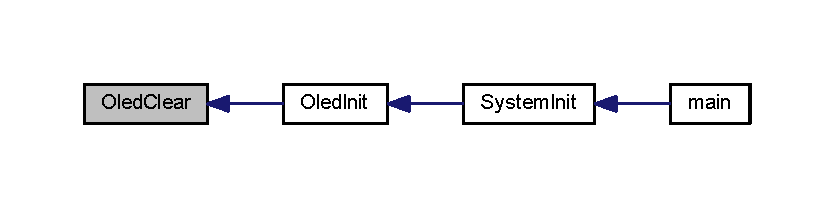
\includegraphics[width=350pt]{group___o_l_e_d_gac33652401561bede6a56b8ff6f9cc16f_icgraph}
\end{center}
\end{figure}


\hypertarget{group___o_l_e_d_ga74eb47866c0626523716f372981e46f9}{\index{\-Bsp\-Oled\-: B\-S\-P Group@{\-Bsp\-Oled\-: B\-S\-P Group}!\-Oled\-Disp@{\-Oled\-Disp}}
\index{\-Oled\-Disp@{\-Oled\-Disp}!BspOled: BSP Group@{\-Bsp\-Oled\-: B\-S\-P Group}}
\subsubsection[{\-Oled\-Disp}]{\setlength{\rightskip}{0pt plus 5cm}void {\bf \-Oled\-Disp} (
\begin{DoxyParamCaption}
\item[{void}]{}
\end{DoxyParamCaption}
)}}\label{group___o_l_e_d_ga74eb47866c0626523716f372981e46f9}


\-O\-L\-E\-D显示一整屏函数 

\-O\-L\-E\-D显示整屏


\begin{DoxyParams}{\-Parameters}
{\em 参数名} & 参数说明 \\
\hline
{\em 无} & \\
\hline
\end{DoxyParams}

\begin{DoxyRetVals}{\-Return values}
{\em 无} & \\
\hline
\end{DoxyRetVals}
\begin{DoxyParagraph}{使用全局变量 }

\end{DoxyParagraph}
\begin{DoxyNote}{\-Note}
● 执行时间\-: \par
 ● 调用周期\-: 触发调用 \par
 ● 可否打断\-: 可以 \par

\end{DoxyNote}
\begin{DoxyParagraph}{注意\-:}
● 无 \par
 
\end{DoxyParagraph}


\-Here is the call graph for this function\-:\nopagebreak
\begin{figure}[H]
\begin{center}
\leavevmode
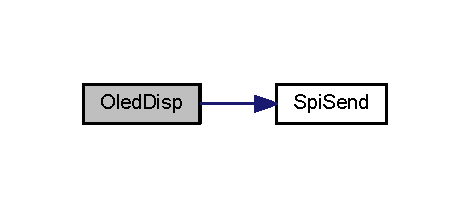
\includegraphics[width=226pt]{group___o_l_e_d_ga74eb47866c0626523716f372981e46f9_cgraph}
\end{center}
\end{figure}


\hypertarget{group___o_l_e_d_ga803969611b487ce2e64bb960be64ad26}{\index{\-Bsp\-Oled\-: B\-S\-P Group@{\-Bsp\-Oled\-: B\-S\-P Group}!\-Oled\-Display@{\-Oled\-Display}}
\index{\-Oled\-Display@{\-Oled\-Display}!BspOled: BSP Group@{\-Bsp\-Oled\-: B\-S\-P Group}}
\subsubsection[{\-Oled\-Display}]{\setlength{\rightskip}{0pt plus 5cm}void {\bf \-Oled\-Display} (
\begin{DoxyParamCaption}
\item[{{\bf u8}}]{x, }
\item[{{\bf u8}}]{y, }
\item[{char}]{width, }
\item[{char}]{hight, }
\item[{{\bf u8} $\ast$}]{data, }
\item[{int}]{x\-Offset, }
\item[{{\bf u8}}]{inverse}
\end{DoxyParamCaption}
)}}\label{group___o_l_e_d_ga803969611b487ce2e64bb960be64ad26}


\-O\-L\-E\-D图片显示函数 


\begin{DoxyParams}[1]{\-Parameters}
 & {\em 参数名} & 参数说明 \\
\hline
\mbox{\tt in}  & {\em x} & x坐标, 0$\sim$127 \\
\hline
\mbox{\tt in}  & {\em y} & y行数, 0$\sim$7 \\
\hline
\mbox{\tt in}  & {\em width} & x宽度, 单位\-:像素 0$\sim$127 \\
\hline
\mbox{\tt in}  & {\em hight} & y宽度, 单位\-:行 0$\sim$7 \\
\hline
\mbox{\tt in}  & {\em data} & 需要显示内容 \\
\hline
\mbox{\tt in}  & {\em x\-Offset} & x轴的偏移, 小于0表示向左偏移, 大于0表示向右偏移 \\
\hline
\mbox{\tt in}  & {\em inverse} & 是否反色 \\
\hline
\end{DoxyParams}

\begin{DoxyRetVals}{\-Return values}
{\em 无} & \\
\hline
\end{DoxyRetVals}
\begin{DoxyParagraph}{使用全局变量 }

\end{DoxyParagraph}
\begin{DoxyNote}{\-Note}
● 执行时间\-: \par
 ● 调用周期\-: 触发调用 \par
 ● 可否打断\-: 可以 \par

\end{DoxyNote}
\begin{DoxyParagraph}{注意\-:}
● 此处只是将要显示的内容加入到显示缓存区中,真正显示由\-Oled\-Disp()来做 \par
 
\end{DoxyParagraph}


\-Here is the caller graph for this function\-:\nopagebreak
\begin{figure}[H]
\begin{center}
\leavevmode
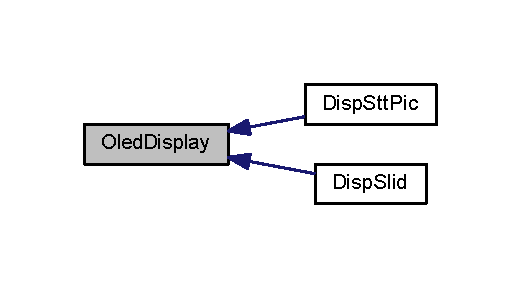
\includegraphics[width=250pt]{group___o_l_e_d_ga803969611b487ce2e64bb960be64ad26_icgraph}
\end{center}
\end{figure}


\hypertarget{group___o_l_e_d_gaad39f47a4a67e81eb4682bc2dc77f7f0}{\index{\-Bsp\-Oled\-: B\-S\-P Group@{\-Bsp\-Oled\-: B\-S\-P Group}!\-Oled\-Display\-Off@{\-Oled\-Display\-Off}}
\index{\-Oled\-Display\-Off@{\-Oled\-Display\-Off}!BspOled: BSP Group@{\-Bsp\-Oled\-: B\-S\-P Group}}
\subsubsection[{\-Oled\-Display\-Off}]{\setlength{\rightskip}{0pt plus 5cm}void {\bf \-Oled\-Display\-Off} (
\begin{DoxyParamCaption}
\item[{void}]{}
\end{DoxyParamCaption}
)}}\label{group___o_l_e_d_gaad39f47a4a67e81eb4682bc2dc77f7f0}


\-O\-L\-E\-D失能显示函数 


\begin{DoxyParams}{\-Parameters}
{\em 参数名} & 参数说明 \\
\hline
{\em 无} & \\
\hline
\end{DoxyParams}

\begin{DoxyRetVals}{\-Return values}
{\em 无} & \\
\hline
\end{DoxyRetVals}
\begin{DoxyParagraph}{使用全局变量 }

\end{DoxyParagraph}
\begin{DoxyNote}{\-Note}
● 执行时间\-: \par
 ● 调用周期\-: 触发调用 \par
 ● 可否打断\-: 可以 \par

\end{DoxyNote}
\begin{DoxyParagraph}{注意\-:}
● 无 \par
 
\end{DoxyParagraph}


\-Here is the caller graph for this function\-:\nopagebreak
\begin{figure}[H]
\begin{center}
\leavevmode
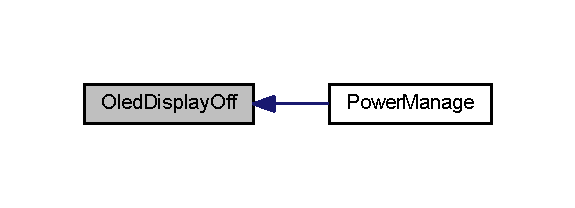
\includegraphics[width=276pt]{group___o_l_e_d_gaad39f47a4a67e81eb4682bc2dc77f7f0_icgraph}
\end{center}
\end{figure}


\hypertarget{group___o_l_e_d_gaa6948206248a6fc7672d9272afb31200}{\index{\-Bsp\-Oled\-: B\-S\-P Group@{\-Bsp\-Oled\-: B\-S\-P Group}!\-Oled\-Display\-On@{\-Oled\-Display\-On}}
\index{\-Oled\-Display\-On@{\-Oled\-Display\-On}!BspOled: BSP Group@{\-Bsp\-Oled\-: B\-S\-P Group}}
\subsubsection[{\-Oled\-Display\-On}]{\setlength{\rightskip}{0pt plus 5cm}void {\bf \-Oled\-Display\-On} (
\begin{DoxyParamCaption}
\item[{void}]{}
\end{DoxyParamCaption}
)}}\label{group___o_l_e_d_gaa6948206248a6fc7672d9272afb31200}


\-O\-L\-E\-D使能显示函数 


\begin{DoxyParams}{\-Parameters}
{\em 参数名} & 参数说明 \\
\hline
{\em 无} & \\
\hline
\end{DoxyParams}

\begin{DoxyRetVals}{\-Return values}
{\em 无} & \\
\hline
\end{DoxyRetVals}
\begin{DoxyParagraph}{使用全局变量 }

\end{DoxyParagraph}
\begin{DoxyNote}{\-Note}
● 执行时间\-: \par
 ● 调用周期\-: 触发调用 \par
 ● 可否打断\-: 可以 \par

\end{DoxyNote}
\begin{DoxyParagraph}{注意\-:}
● 无 \par
 
\end{DoxyParagraph}


\-Here is the caller graph for this function\-:\nopagebreak
\begin{figure}[H]
\begin{center}
\leavevmode
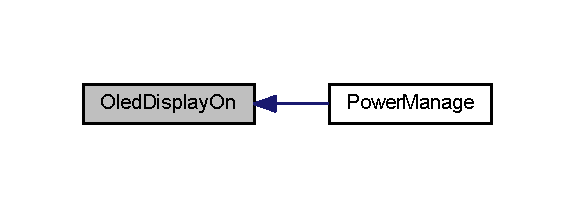
\includegraphics[width=276pt]{group___o_l_e_d_gaa6948206248a6fc7672d9272afb31200_icgraph}
\end{center}
\end{figure}


\hypertarget{group___o_l_e_d_ga11720eb1002774b7a17f14b56ff44af8}{\index{\-Bsp\-Oled\-: B\-S\-P Group@{\-Bsp\-Oled\-: B\-S\-P Group}!\-Oled\-Init@{\-Oled\-Init}}
\index{\-Oled\-Init@{\-Oled\-Init}!BspOled: BSP Group@{\-Bsp\-Oled\-: B\-S\-P Group}}
\subsubsection[{\-Oled\-Init}]{\setlength{\rightskip}{0pt plus 5cm}void {\bf \-Oled\-Init} (
\begin{DoxyParamCaption}
\item[{void}]{}
\end{DoxyParamCaption}
)}}\label{group___o_l_e_d_ga11720eb1002774b7a17f14b56ff44af8}


\-O\-L\-E\-D初始化函数 


\begin{DoxyParams}{\-Parameters}
{\em 参数名} & 参数说明 \\
\hline
{\em 无} & \\
\hline
\end{DoxyParams}

\begin{DoxyRetVals}{\-Return values}
{\em 无} & \\
\hline
\end{DoxyRetVals}
\begin{DoxyParagraph}{使用全局变量 }

\end{DoxyParagraph}
\begin{DoxyNote}{\-Note}
● 执行时间\-: \par
 ● 调用周期\-: 触发调用, 初始化时调用 \par
 ● 可否打断\-: 可以 \par

\end{DoxyNote}
\begin{DoxyParagraph}{注意\-:}
● 无 \par
 
\end{DoxyParagraph}


\-Here is the call graph for this function\-:\nopagebreak
\begin{figure}[H]
\begin{center}
\leavevmode
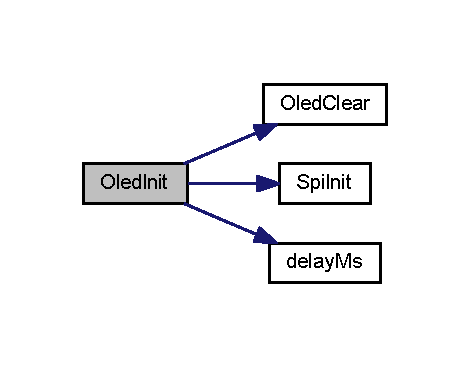
\includegraphics[width=226pt]{group___o_l_e_d_ga11720eb1002774b7a17f14b56ff44af8_cgraph}
\end{center}
\end{figure}




\-Here is the caller graph for this function\-:\nopagebreak
\begin{figure}[H]
\begin{center}
\leavevmode
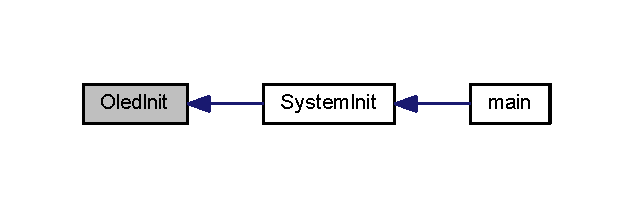
\includegraphics[width=304pt]{group___o_l_e_d_ga11720eb1002774b7a17f14b56ff44af8_icgraph}
\end{center}
\end{figure}


\hypertarget{group___o_l_e_d_ga0e199e6945e270291c54aedda692d48c}{\index{\-Bsp\-Oled\-: B\-S\-P Group@{\-Bsp\-Oled\-: B\-S\-P Group}!\-Oled\-Show\-String@{\-Oled\-Show\-String}}
\index{\-Oled\-Show\-String@{\-Oled\-Show\-String}!BspOled: BSP Group@{\-Bsp\-Oled\-: B\-S\-P Group}}
\subsubsection[{\-Oled\-Show\-String}]{\setlength{\rightskip}{0pt plus 5cm}void {\bf \-Oled\-Show\-String} (
\begin{DoxyParamCaption}
\item[{{\bf u8}}]{x, }
\item[{{\bf u8}}]{y, }
\item[{char $\ast$}]{chr, }
\item[{int}]{x\-Offset, }
\item[{{\bf u8}}]{inverse}
\end{DoxyParamCaption}
)}}\label{group___o_l_e_d_ga0e199e6945e270291c54aedda692d48c}


\-O\-L\-E\-D字符串显示函数 


\begin{DoxyParams}[1]{\-Parameters}
 & {\em 参数名} & 参数说明 \\
\hline
\mbox{\tt in}  & {\em x} & x坐标, 0$\sim$127 \\
\hline
\mbox{\tt in}  & {\em y} & y行数, 0$\sim$7 \\
\hline
\mbox{\tt in}  & {\em chr} & 需要显示的字符串指针 \\
\hline
\mbox{\tt in}  & {\em x\-Offset} & x轴的偏移, 小于0表示向左偏移, 大于0表示向右偏移 \\
\hline
\mbox{\tt in}  & {\em inverse} & 是否反色 \\
\hline
\end{DoxyParams}

\begin{DoxyRetVals}{\-Return values}
{\em 无} & \\
\hline
\end{DoxyRetVals}
\begin{DoxyParagraph}{使用全局变量 }

\end{DoxyParagraph}
\begin{DoxyNote}{\-Note}
● 执行时间\-: \par
 ● 调用周期\-: 触发调用 \par
 ● 可否打断\-: 可以 \par

\end{DoxyNote}
\begin{DoxyParagraph}{注意\-:}
● 无 \par
 
\end{DoxyParagraph}


\-Here is the caller graph for this function\-:\nopagebreak
\begin{figure}[H]
\begin{center}
\leavevmode
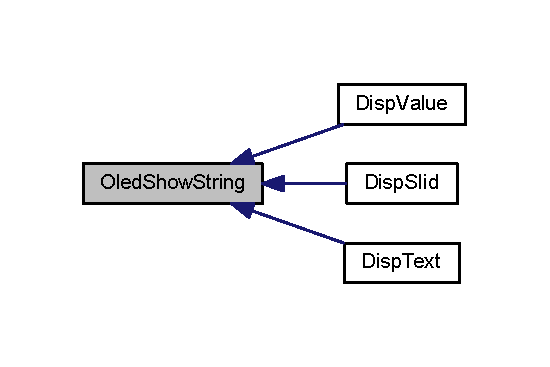
\includegraphics[width=264pt]{group___o_l_e_d_ga0e199e6945e270291c54aedda692d48c_icgraph}
\end{center}
\end{figure}



\hypertarget{group___r_t_c}{\section{\-Bsp\-Rtc\-: \-B\-S\-P \-Group}
\label{group___r_t_c}\index{\-Bsp\-Rtc\-: B\-S\-P Group@{\-Bsp\-Rtc\-: B\-S\-P Group}}
}
\subsection*{\-Data \-Structures}
\begin{DoxyCompactItemize}
\item 
struct \hyperlink{struct_s_t_r___time}{\-S\-T\-R\-\_\-\-Time}
\begin{DoxyCompactList}\small\item\em 时间结构体 \end{DoxyCompactList}\item 
struct \hyperlink{struct_s_t_r___rtc}{\-S\-T\-R\-\_\-\-Rtc}
\begin{DoxyCompactList}\small\item\em 实时时钟结构体 \end{DoxyCompactList}\end{DoxyCompactItemize}
\subsection*{\-Defines}
\begin{DoxyCompactItemize}
\item 
\hypertarget{group___r_t_c_gafd32b987540dc4ff9a42b0f38f5714e2}{\#define \hyperlink{group___r_t_c_gafd32b987540dc4ff9a42b0f38f5714e2}{\-R\-X8025\-\_\-\-A\-D\-D\-R}~0x64}\label{group___r_t_c_gafd32b987540dc4ff9a42b0f38f5714e2}

\begin{DoxyCompactList}\small\item\em \-I2\-C设备地址 \end{DoxyCompactList}\item 
\#define \hyperlink{group___r_t_c_ga8c3426877a1caf234a667f0c0e58fd2e}{\-R\-X8025\-\_\-\-A\-D\-D\-R\-\_\-\-S\-E\-C\-O\-N\-D\-S}~0x00
\begin{DoxyCompactList}\small\item\em 设备寄存器地址 \end{DoxyCompactList}\item 
\hypertarget{group___r_t_c_ga3ee94c0bc1a53d58526f48b41ed44d2f}{\#define \hyperlink{group___r_t_c_ga3ee94c0bc1a53d58526f48b41ed44d2f}{\-R\-X8025\-\_\-\-A\-D\-D\-R\-\_\-\-W\-E\-E\-K}~0x30}\label{group___r_t_c_ga3ee94c0bc1a53d58526f48b41ed44d2f}

\begin{DoxyCompactList}\small\item\em 星期寄存器 \end{DoxyCompactList}\item 
\hypertarget{group___r_t_c_ga0f805e684493aa7d586ff1fac6b794e6}{\#define \hyperlink{group___r_t_c_ga0f805e684493aa7d586ff1fac6b794e6}{\-R\-X8025\-\_\-\-A\-D\-D\-R\-\_\-\-D\-A\-T\-E\-S}~0x40}\label{group___r_t_c_ga0f805e684493aa7d586ff1fac6b794e6}

\begin{DoxyCompactList}\small\item\em 日期寄存器 \end{DoxyCompactList}\item 
\hypertarget{group___r_t_c_ga561666ebab18081a04d0a64fd9d1805d}{\#define \hyperlink{group___r_t_c_ga561666ebab18081a04d0a64fd9d1805d}{\-R\-X8025\-\_\-\-A\-D\-D\-R\-\_\-\-M\-O\-N\-T\-H}~0x50}\label{group___r_t_c_ga561666ebab18081a04d0a64fd9d1805d}

\begin{DoxyCompactList}\small\item\em 月寄存器 \end{DoxyCompactList}\item 
\hypertarget{group___r_t_c_ga303d3794c823d33caf68cc580c6344a9}{\#define \hyperlink{group___r_t_c_ga303d3794c823d33caf68cc580c6344a9}{\-R\-X8025\-\_\-\-A\-D\-D\-R\-\_\-\-M\-I\-N\-U\-T\-E\-S}~0x80}\label{group___r_t_c_ga303d3794c823d33caf68cc580c6344a9}

\begin{DoxyCompactList}\small\item\em 分钟寄存器 \end{DoxyCompactList}\item 
\hypertarget{group___r_t_c_gaed871931d582bd8e566fe78ab63de303}{\#define \hyperlink{group___r_t_c_gaed871931d582bd8e566fe78ab63de303}{\-R\-X8025\-\_\-\-A\-D\-D\-R\-\_\-\-E\-X\-T\-E\-N\-S\-I\-O\-N}~0x\-D0}\label{group___r_t_c_gaed871931d582bd8e566fe78ab63de303}

\begin{DoxyCompactList}\small\item\em 扩展寄存器 \end{DoxyCompactList}\item 
\hypertarget{group___r_t_c_ga1aff3dd19320a3ba36ac48fe1af6eeb7}{\#define \hyperlink{group___r_t_c_ga1aff3dd19320a3ba36ac48fe1af6eeb7}{\-R\-X8025\-\_\-\-A\-D\-D\-R\-\_\-\-F\-L\-A\-G}~0x\-E0}\label{group___r_t_c_ga1aff3dd19320a3ba36ac48fe1af6eeb7}

\begin{DoxyCompactList}\small\item\em 标志位寄存器 \end{DoxyCompactList}\item 
\hypertarget{group___r_t_c_ga3462d91191aa01f9d3605bde19cc418d}{\#define \hyperlink{group___r_t_c_ga3462d91191aa01f9d3605bde19cc418d}{\-R\-X8025\-\_\-\-A\-D\-D\-R\-\_\-\-C\-O\-N\-T\-R\-O\-L}~0x\-F0}\label{group___r_t_c_ga3462d91191aa01f9d3605bde19cc418d}

\begin{DoxyCompactList}\small\item\em 控制寄存器 \end{DoxyCompactList}\item 
\#define \hyperlink{group___r_t_c_ga85b5a97fce88a05c8211049ab07be590}{\-R\-X8025\-\_\-\-W\-R\-I\-T\-E\-\_\-\-M\-O\-D\-E}~0x\-F0
\begin{DoxyCompactList}\small\item\em 设备操作模式 \end{DoxyCompactList}\item 
\hypertarget{group___r_t_c_ga783718aa6e959ed6f154c56060438164}{\#define \hyperlink{group___r_t_c_ga783718aa6e959ed6f154c56060438164}{\-R\-X8025\-\_\-\-R\-E\-A\-D\-\_\-\-M\-O\-D\-E}~0x\-F0}\label{group___r_t_c_ga783718aa6e959ed6f154c56060438164}

\begin{DoxyCompactList}\small\item\em 读模式 \end{DoxyCompactList}\item 
\#define \hyperlink{group___r_t_c_ga6764dc0bd7e59b4eca8d525f8136fd86}{\-S\-U\-N\-D\-A\-Y}~0x01
\begin{DoxyCompactList}\small\item\em 星期设置 \end{DoxyCompactList}\item 
\hypertarget{group___r_t_c_ga7170de6ea0ab27a44b607e025eeda10b}{\#define \hyperlink{group___r_t_c_ga7170de6ea0ab27a44b607e025eeda10b}{\-M\-O\-N\-D\-A\-Y}~0x02}\label{group___r_t_c_ga7170de6ea0ab27a44b607e025eeda10b}

\begin{DoxyCompactList}\small\item\em 周一 \end{DoxyCompactList}\item 
\hypertarget{group___r_t_c_ga7e614639937b5dc668fb843882ddf895}{\#define \hyperlink{group___r_t_c_ga7e614639937b5dc668fb843882ddf895}{\-T\-U\-E\-S\-D\-A\-Y}~0x04}\label{group___r_t_c_ga7e614639937b5dc668fb843882ddf895}

\begin{DoxyCompactList}\small\item\em 周二 \end{DoxyCompactList}\item 
\hypertarget{group___r_t_c_gabc50400fb4fc6d0b982a22b5e9644a8c}{\#define \hyperlink{group___r_t_c_gabc50400fb4fc6d0b982a22b5e9644a8c}{\-W\-E\-D\-N\-E\-S\-D\-A\-Y}~0x08}\label{group___r_t_c_gabc50400fb4fc6d0b982a22b5e9644a8c}

\begin{DoxyCompactList}\small\item\em 周三 \end{DoxyCompactList}\item 
\hypertarget{group___r_t_c_ga4383b2bef864f3be7c45bdbfced40e4d}{\#define \hyperlink{group___r_t_c_ga4383b2bef864f3be7c45bdbfced40e4d}{\-T\-H\-U\-R\-S\-D\-A\-Y}~0x10}\label{group___r_t_c_ga4383b2bef864f3be7c45bdbfced40e4d}

\begin{DoxyCompactList}\small\item\em 周四 \end{DoxyCompactList}\item 
\hypertarget{group___r_t_c_gabe9db6f3a1fb60fa435c899c00dd0987}{\#define \hyperlink{group___r_t_c_gabe9db6f3a1fb60fa435c899c00dd0987}{\-F\-R\-I\-D\-A\-Y}~0x20}\label{group___r_t_c_gabe9db6f3a1fb60fa435c899c00dd0987}

\begin{DoxyCompactList}\small\item\em 周五 \end{DoxyCompactList}\item 
\hypertarget{group___r_t_c_gab211cb1e7ca439c7d2c6cc675b0dcc88}{\#define \hyperlink{group___r_t_c_gab211cb1e7ca439c7d2c6cc675b0dcc88}{\-S\-A\-T\-U\-R\-D\-A\-Y}~0x40}\label{group___r_t_c_gab211cb1e7ca439c7d2c6cc675b0dcc88}

\begin{DoxyCompactList}\small\item\em 周六 \end{DoxyCompactList}\end{DoxyCompactItemize}
\subsection*{\-Functions}
\begin{DoxyCompactItemize}
\item 
void \hyperlink{group___r_t_c_gaa884644b359833678d1f4bde7c214e32}{\-Rtc\-Init} (void)
\begin{DoxyCompactList}\small\item\em 实时时钟初始化函数 \end{DoxyCompactList}\item 
\hyperlink{group___b_s_p_gaed742c436da53c1080638ce6ef7d13de}{u8} \hyperlink{group___r_t_c_gad69809279bbf3aba7d8e066605e8950d}{\-Time\-Set} (\hyperlink{struct_s_t_r___time}{\-S\-T\-R\-\_\-\-Time} $\ast$time)
\begin{DoxyCompactList}\small\item\em 设置时间 \end{DoxyCompactList}\item 
\hyperlink{group___b_s_p_gaed742c436da53c1080638ce6ef7d13de}{u8} \hyperlink{group___r_t_c_gad9a05048b632c9b164c3735a93a07e98}{\-Get\-Time} (\hyperlink{struct_s_t_r___time}{\-S\-T\-R\-\_\-\-Time} $\ast$time)
\begin{DoxyCompactList}\small\item\em 读取时间 \end{DoxyCompactList}\item 
void \hyperlink{group___r_t_c_gad63ba0576495490f98a46bbd85e9ad49}{\-Read\-Time\-D\-M\-A} (\hyperlink{struct_s_t_r___rtc}{\-S\-T\-R\-\_\-\-Rtc} $\ast$rtc)
\begin{DoxyCompactList}\small\item\em 读取时间 \end{DoxyCompactList}\item 
void \hyperlink{group___r_t_c_gaf889c27a181d6c5c14b9c3e0c5a3e58f}{\-Get\-Time\-D\-M\-A} (\hyperlink{struct_s_t_r___rtc}{\-S\-T\-R\-\_\-\-Rtc} $\ast$rtc)
\begin{DoxyCompactList}\small\item\em 读取时间 \end{DoxyCompactList}\item 
void \hyperlink{group___r_t_c_gab14f1be5febcc98f825a51a2ed15e7fc}{\-Get\-Time\-String} (\hyperlink{struct_s_t_r___time}{\-S\-T\-R\-\_\-\-Time} $\ast$time, char $\ast$string)
\begin{DoxyCompactList}\small\item\em 获取时间字符串用于显示 \end{DoxyCompactList}\item 
void \hyperlink{group___r_t_c_ga4f14b7b7736d3f689f1abecd195458f1}{\-Get\-Date\-String} (\hyperlink{struct_s_t_r___time}{\-S\-T\-R\-\_\-\-Time} $\ast$time, char $\ast$string)
\begin{DoxyCompactList}\small\item\em 获取日期字符串用于显示 \end{DoxyCompactList}\item 
\hypertarget{group___r_t_c_gac03799b56ed83e28e102088590349d25}{\hyperlink{group___b_s_p_gaed742c436da53c1080638ce6ef7d13de}{u8} \hyperlink{group___r_t_c_gac03799b56ed83e28e102088590349d25}{\-Time\-Read} (\hyperlink{struct_s_t_r___time}{\-S\-T\-R\-\_\-\-Time} $\ast$time)}\label{group___r_t_c_gac03799b56ed83e28e102088590349d25}

\begin{DoxyCompactList}\small\item\em 读取时间 \end{DoxyCompactList}\end{DoxyCompactItemize}
\subsection*{\-Variables}
\begin{DoxyCompactItemize}
\item 
\hypertarget{group___r_t_c_gac4564180c5a6381255467f7e41f2fdc0}{\hyperlink{struct_s_t_r___rtc}{\-S\-T\-R\-\_\-\-Rtc} \hyperlink{group___r_t_c_gac4564180c5a6381255467f7e41f2fdc0}{\-Rtc}}\label{group___r_t_c_gac4564180c5a6381255467f7e41f2fdc0}

\begin{DoxyCompactList}\small\item\em 实时时钟结构体 \end{DoxyCompactList}\item 
\hypertarget{group___r_t_c_gac4564180c5a6381255467f7e41f2fdc0}{\hyperlink{struct_s_t_r___rtc}{\-S\-T\-R\-\_\-\-Rtc} \hyperlink{group___r_t_c_gac4564180c5a6381255467f7e41f2fdc0}{\-Rtc}}\label{group___r_t_c_gac4564180c5a6381255467f7e41f2fdc0}

\begin{DoxyCompactList}\small\item\em 实时时钟结构体 \end{DoxyCompactList}\end{DoxyCompactItemize}


\subsection{\-Define \-Documentation}
\hypertarget{group___r_t_c_ga8c3426877a1caf234a667f0c0e58fd2e}{\index{\-Bsp\-Rtc\-: B\-S\-P Group@{\-Bsp\-Rtc\-: B\-S\-P Group}!\-R\-X8025\-\_\-\-A\-D\-D\-R\-\_\-\-S\-E\-C\-O\-N\-D\-S@{\-R\-X8025\-\_\-\-A\-D\-D\-R\-\_\-\-S\-E\-C\-O\-N\-D\-S}}
\index{\-R\-X8025\-\_\-\-A\-D\-D\-R\-\_\-\-S\-E\-C\-O\-N\-D\-S@{\-R\-X8025\-\_\-\-A\-D\-D\-R\-\_\-\-S\-E\-C\-O\-N\-D\-S}!BspRtc: BSP Group@{\-Bsp\-Rtc\-: B\-S\-P Group}}
\subsubsection[{\-R\-X8025\-\_\-\-A\-D\-D\-R\-\_\-\-S\-E\-C\-O\-N\-D\-S}]{\setlength{\rightskip}{0pt plus 5cm}\#define {\bf \-R\-X8025\-\_\-\-A\-D\-D\-R\-\_\-\-S\-E\-C\-O\-N\-D\-S}~0x00}}\label{group___r_t_c_ga8c3426877a1caf234a667f0c0e58fd2e}


设备寄存器地址 

秒寄存器 \hypertarget{group___r_t_c_ga85b5a97fce88a05c8211049ab07be590}{\index{\-Bsp\-Rtc\-: B\-S\-P Group@{\-Bsp\-Rtc\-: B\-S\-P Group}!\-R\-X8025\-\_\-\-W\-R\-I\-T\-E\-\_\-\-M\-O\-D\-E@{\-R\-X8025\-\_\-\-W\-R\-I\-T\-E\-\_\-\-M\-O\-D\-E}}
\index{\-R\-X8025\-\_\-\-W\-R\-I\-T\-E\-\_\-\-M\-O\-D\-E@{\-R\-X8025\-\_\-\-W\-R\-I\-T\-E\-\_\-\-M\-O\-D\-E}!BspRtc: BSP Group@{\-Bsp\-Rtc\-: B\-S\-P Group}}
\subsubsection[{\-R\-X8025\-\_\-\-W\-R\-I\-T\-E\-\_\-\-M\-O\-D\-E}]{\setlength{\rightskip}{0pt plus 5cm}\#define {\bf \-R\-X8025\-\_\-\-W\-R\-I\-T\-E\-\_\-\-M\-O\-D\-E}~0x\-F0}}\label{group___r_t_c_ga85b5a97fce88a05c8211049ab07be590}


设备操作模式 

写模式 \hypertarget{group___r_t_c_ga6764dc0bd7e59b4eca8d525f8136fd86}{\index{\-Bsp\-Rtc\-: B\-S\-P Group@{\-Bsp\-Rtc\-: B\-S\-P Group}!\-S\-U\-N\-D\-A\-Y@{\-S\-U\-N\-D\-A\-Y}}
\index{\-S\-U\-N\-D\-A\-Y@{\-S\-U\-N\-D\-A\-Y}!BspRtc: BSP Group@{\-Bsp\-Rtc\-: B\-S\-P Group}}
\subsubsection[{\-S\-U\-N\-D\-A\-Y}]{\setlength{\rightskip}{0pt plus 5cm}\#define {\bf \-S\-U\-N\-D\-A\-Y}~0x01}}\label{group___r_t_c_ga6764dc0bd7e59b4eca8d525f8136fd86}


星期设置 

周日 

\subsection{\-Function \-Documentation}
\hypertarget{group___r_t_c_ga4f14b7b7736d3f689f1abecd195458f1}{\index{\-Bsp\-Rtc\-: B\-S\-P Group@{\-Bsp\-Rtc\-: B\-S\-P Group}!\-Get\-Date\-String@{\-Get\-Date\-String}}
\index{\-Get\-Date\-String@{\-Get\-Date\-String}!BspRtc: BSP Group@{\-Bsp\-Rtc\-: B\-S\-P Group}}
\subsubsection[{\-Get\-Date\-String}]{\setlength{\rightskip}{0pt plus 5cm}void {\bf \-Get\-Date\-String} (
\begin{DoxyParamCaption}
\item[{{\bf \-S\-T\-R\-\_\-\-Time} $\ast$}]{time, }
\item[{char $\ast$}]{string}
\end{DoxyParamCaption}
)}}\label{group___r_t_c_ga4f14b7b7736d3f689f1abecd195458f1}


获取日期字符串用于显示 


\begin{DoxyParams}[1]{\-Parameters}
 & {\em 参数名} & 参数说明 \\
\hline
\mbox{\tt in}  & {\em time} & 时间结构体指针 \\
\hline
\mbox{\tt out}  & {\em string} & 字符串指针 \\
\hline
\end{DoxyParams}

\begin{DoxyRetVals}{\-Return values}
{\em 0-\/失败} & 1-\/成功 \\
\hline
\end{DoxyRetVals}
\begin{DoxyParagraph}{使用全局变量 }

\end{DoxyParagraph}
\begin{DoxyNote}{\-Note}
● 执行时间\-: \par
 ● 调用周期\-: 100ms调用 \par
 ● 可否打断\-: 可以 \par

\end{DoxyNote}
\begin{DoxyParagraph}{注意\-:}
● 无 \par
 
\end{DoxyParagraph}
\hypertarget{group___r_t_c_gad9a05048b632c9b164c3735a93a07e98}{\index{\-Bsp\-Rtc\-: B\-S\-P Group@{\-Bsp\-Rtc\-: B\-S\-P Group}!\-Get\-Time@{\-Get\-Time}}
\index{\-Get\-Time@{\-Get\-Time}!BspRtc: BSP Group@{\-Bsp\-Rtc\-: B\-S\-P Group}}
\subsubsection[{\-Get\-Time}]{\setlength{\rightskip}{0pt plus 5cm}{\bf u8} {\bf \-Get\-Time} (
\begin{DoxyParamCaption}
\item[{{\bf \-S\-T\-R\-\_\-\-Time} $\ast$}]{time}
\end{DoxyParamCaption}
)}}\label{group___r_t_c_gad9a05048b632c9b164c3735a93a07e98}


读取时间 


\begin{DoxyParams}[1]{\-Parameters}
 & {\em 参数名} & 参数说明 \\
\hline
\mbox{\tt out}  & {\em time} & 时间结构体指针 \\
\hline
\end{DoxyParams}

\begin{DoxyRetVals}{\-Return values}
{\em 0-\/失败} & 1-\/成功 \\
\hline
\end{DoxyRetVals}
\begin{DoxyParagraph}{使用全局变量 }

\end{DoxyParagraph}
\begin{DoxyNote}{\-Note}
● 执行时间\-: \par
 ● 调用周期\-: 100ms调用 \par
 ● 可否打断\-: 可以 \par

\end{DoxyNote}
\begin{DoxyParagraph}{注意\-:}
● 等待方式\-I2\-C读取数据,耗时较长,2.0以上版本已经不再使用 \par
 
\end{DoxyParagraph}


\-Here is the call graph for this function\-:\nopagebreak
\begin{figure}[H]
\begin{center}
\leavevmode
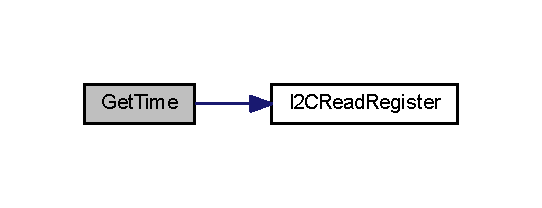
\includegraphics[width=260pt]{group___r_t_c_gad9a05048b632c9b164c3735a93a07e98_cgraph}
\end{center}
\end{figure}


\hypertarget{group___r_t_c_gaf889c27a181d6c5c14b9c3e0c5a3e58f}{\index{\-Bsp\-Rtc\-: B\-S\-P Group@{\-Bsp\-Rtc\-: B\-S\-P Group}!\-Get\-Time\-D\-M\-A@{\-Get\-Time\-D\-M\-A}}
\index{\-Get\-Time\-D\-M\-A@{\-Get\-Time\-D\-M\-A}!BspRtc: BSP Group@{\-Bsp\-Rtc\-: B\-S\-P Group}}
\subsubsection[{\-Get\-Time\-D\-M\-A}]{\setlength{\rightskip}{0pt plus 5cm}void {\bf \-Get\-Time\-D\-M\-A} (
\begin{DoxyParamCaption}
\item[{{\bf \-S\-T\-R\-\_\-\-Rtc} $\ast$}]{rtc}
\end{DoxyParamCaption}
)}}\label{group___r_t_c_gaf889c27a181d6c5c14b9c3e0c5a3e58f}


读取时间 


\begin{DoxyParams}[1]{\-Parameters}
 & {\em 参数名} & 参数说明 \\
\hline
\mbox{\tt out}  & {\em rtc} & 时间结构体指针 \\
\hline
\end{DoxyParams}

\begin{DoxyRetVals}{\-Return values}
{\em 无} & \\
\hline
\end{DoxyRetVals}
\begin{DoxyParagraph}{使用全局变量 }

\end{DoxyParagraph}
\begin{DoxyNote}{\-Note}
● 执行时间\-: \par
 ● 调用周期\-: 100ms调用 \par
 ● 可否打断\-: 可以 \par

\end{DoxyNote}
\begin{DoxyParagraph}{注意\-:}
● 根据\-Time\-Now.\-i2c\-Buf中读到的寄存器值, 更新时间结构体中的各个变量 \par
 
\end{DoxyParagraph}
\hypertarget{group___r_t_c_gab14f1be5febcc98f825a51a2ed15e7fc}{\index{\-Bsp\-Rtc\-: B\-S\-P Group@{\-Bsp\-Rtc\-: B\-S\-P Group}!\-Get\-Time\-String@{\-Get\-Time\-String}}
\index{\-Get\-Time\-String@{\-Get\-Time\-String}!BspRtc: BSP Group@{\-Bsp\-Rtc\-: B\-S\-P Group}}
\subsubsection[{\-Get\-Time\-String}]{\setlength{\rightskip}{0pt plus 5cm}void {\bf \-Get\-Time\-String} (
\begin{DoxyParamCaption}
\item[{{\bf \-S\-T\-R\-\_\-\-Time} $\ast$}]{time, }
\item[{char $\ast$}]{string}
\end{DoxyParamCaption}
)}}\label{group___r_t_c_gab14f1be5febcc98f825a51a2ed15e7fc}


获取时间字符串用于显示 


\begin{DoxyParams}[1]{\-Parameters}
 & {\em 参数名} & 参数说明 \\
\hline
\mbox{\tt in}  & {\em time} & 时间结构体指针 \\
\hline
\mbox{\tt out}  & {\em string} & 字符串指针 \\
\hline
\end{DoxyParams}

\begin{DoxyRetVals}{\-Return values}
{\em 0-\/失败} & 1-\/成功 \\
\hline
\end{DoxyRetVals}
\begin{DoxyParagraph}{使用全局变量 }

\end{DoxyParagraph}
\begin{DoxyNote}{\-Note}
● 执行时间\-: \par
 ● 调用周期\-: 100ms调用 \par
 ● 可否打断\-: 可以 \par

\end{DoxyNote}
\begin{DoxyParagraph}{注意\-:}
● 无 \par
 
\end{DoxyParagraph}
\hypertarget{group___r_t_c_gad63ba0576495490f98a46bbd85e9ad49}{\index{\-Bsp\-Rtc\-: B\-S\-P Group@{\-Bsp\-Rtc\-: B\-S\-P Group}!\-Read\-Time\-D\-M\-A@{\-Read\-Time\-D\-M\-A}}
\index{\-Read\-Time\-D\-M\-A@{\-Read\-Time\-D\-M\-A}!BspRtc: BSP Group@{\-Bsp\-Rtc\-: B\-S\-P Group}}
\subsubsection[{\-Read\-Time\-D\-M\-A}]{\setlength{\rightskip}{0pt plus 5cm}void {\bf \-Read\-Time\-D\-M\-A} (
\begin{DoxyParamCaption}
\item[{{\bf \-S\-T\-R\-\_\-\-Rtc} $\ast$}]{rtc}
\end{DoxyParamCaption}
)}}\label{group___r_t_c_gad63ba0576495490f98a46bbd85e9ad49}


读取时间 


\begin{DoxyParams}[1]{\-Parameters}
 & {\em 参数名} & 参数说明 \\
\hline
\mbox{\tt out}  & {\em rtc} & 时间结构体指针 \\
\hline
\end{DoxyParams}

\begin{DoxyRetVals}{\-Return values}
{\em 无} & \\
\hline
\end{DoxyRetVals}
\begin{DoxyParagraph}{使用全局变量 }

\end{DoxyParagraph}
\begin{DoxyNote}{\-Note}
● 执行时间\-: \par
 ● 调用周期\-: 100ms调用 \par
 ● 可否打断\-: 可以 \par

\end{DoxyNote}
\begin{DoxyParagraph}{注意\-:}
● 通过\-D\-M\-A \-I2\-C读取\-R\-X8025的寄存器,结果存储在\-Time\-Now.\-i2c\-Buf中 \par
 
\end{DoxyParagraph}


\-Here is the call graph for this function\-:\nopagebreak
\begin{figure}[H]
\begin{center}
\leavevmode
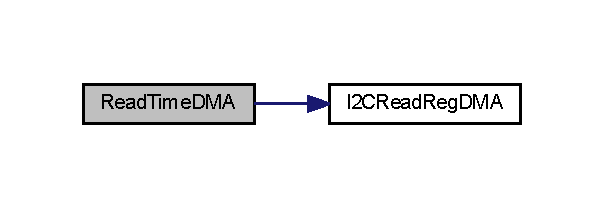
\includegraphics[width=290pt]{group___r_t_c_gad63ba0576495490f98a46bbd85e9ad49_cgraph}
\end{center}
\end{figure}


\hypertarget{group___r_t_c_gaa884644b359833678d1f4bde7c214e32}{\index{\-Bsp\-Rtc\-: B\-S\-P Group@{\-Bsp\-Rtc\-: B\-S\-P Group}!\-Rtc\-Init@{\-Rtc\-Init}}
\index{\-Rtc\-Init@{\-Rtc\-Init}!BspRtc: BSP Group@{\-Bsp\-Rtc\-: B\-S\-P Group}}
\subsubsection[{\-Rtc\-Init}]{\setlength{\rightskip}{0pt plus 5cm}void {\bf \-Rtc\-Init} (
\begin{DoxyParamCaption}
\item[{void}]{}
\end{DoxyParamCaption}
)}}\label{group___r_t_c_gaa884644b359833678d1f4bde7c214e32}


实时时钟初始化函数 

实时时钟初始函数


\begin{DoxyParams}{\-Parameters}
{\em 参数名} & 参数说明 \\
\hline
{\em 无} & \\
\hline
\end{DoxyParams}

\begin{DoxyRetVals}{\-Return values}
{\em 无} & \\
\hline
\end{DoxyRetVals}
\begin{DoxyParagraph}{使用全局变量 }

\end{DoxyParagraph}
\begin{DoxyNote}{\-Note}
● 执行时间\-: \par
 ● 调用周期\-: 触发调用, 初始化时调用 \par
 ● 可否打断\-: 可以 \par

\end{DoxyNote}
\begin{DoxyParagraph}{注意\-:}
● 无 \par
 
\end{DoxyParagraph}


\-Here is the call graph for this function\-:\nopagebreak
\begin{figure}[H]
\begin{center}
\leavevmode
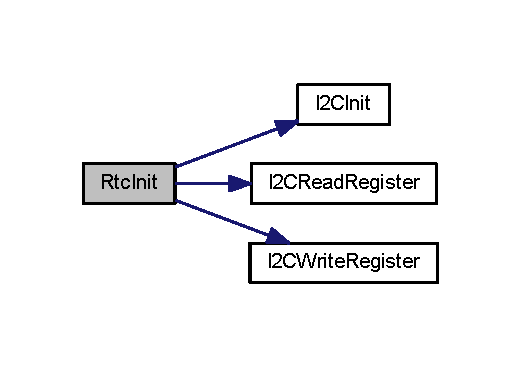
\includegraphics[width=250pt]{group___r_t_c_gaa884644b359833678d1f4bde7c214e32_cgraph}
\end{center}
\end{figure}




\-Here is the caller graph for this function\-:\nopagebreak
\begin{figure}[H]
\begin{center}
\leavevmode
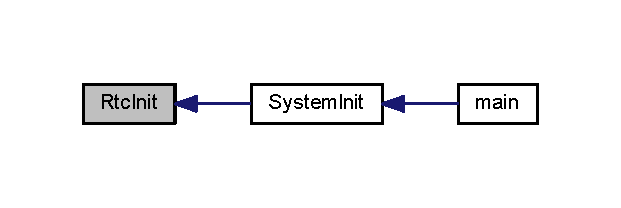
\includegraphics[width=298pt]{group___r_t_c_gaa884644b359833678d1f4bde7c214e32_icgraph}
\end{center}
\end{figure}


\hypertarget{group___r_t_c_gad69809279bbf3aba7d8e066605e8950d}{\index{\-Bsp\-Rtc\-: B\-S\-P Group@{\-Bsp\-Rtc\-: B\-S\-P Group}!\-Time\-Set@{\-Time\-Set}}
\index{\-Time\-Set@{\-Time\-Set}!BspRtc: BSP Group@{\-Bsp\-Rtc\-: B\-S\-P Group}}
\subsubsection[{\-Time\-Set}]{\setlength{\rightskip}{0pt plus 5cm}{\bf u8} {\bf \-Time\-Set} (
\begin{DoxyParamCaption}
\item[{{\bf \-S\-T\-R\-\_\-\-Time} $\ast$}]{time}
\end{DoxyParamCaption}
)}}\label{group___r_t_c_gad69809279bbf3aba7d8e066605e8950d}


设置时间 


\begin{DoxyParams}[1]{\-Parameters}
 & {\em 参数名} & 参数说明 \\
\hline
\mbox{\tt in}  & {\em time} & 时间结构体指针 \\
\hline
\end{DoxyParams}

\begin{DoxyRetVals}{\-Return values}
{\em 0-\/失败} & 1-\/成功 \\
\hline
\end{DoxyRetVals}
\begin{DoxyParagraph}{使用全局变量 }

\end{DoxyParagraph}
\begin{DoxyNote}{\-Note}
● 执行时间\-: \par
 ● 调用周期\-: 触发调用 \par
 ● 可否打断\-: 可以 \par

\end{DoxyNote}
\begin{DoxyParagraph}{注意\-:}
● \par
 
\end{DoxyParagraph}


\-Here is the call graph for this function\-:\nopagebreak
\begin{figure}[H]
\begin{center}
\leavevmode
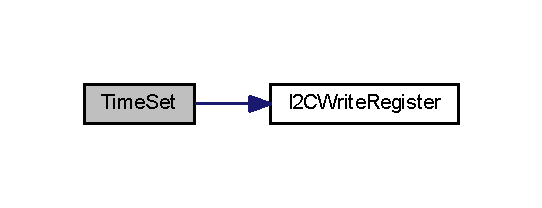
\includegraphics[width=260pt]{group___r_t_c_gad69809279bbf3aba7d8e066605e8950d_cgraph}
\end{center}
\end{figure}



\hypertarget{group___t_e_m_p}{\section{\-Bsp\-Temp\-: \-B\-S\-P \-Group}
\label{group___t_e_m_p}\index{\-Bsp\-Temp\-: B\-S\-P Group@{\-Bsp\-Temp\-: B\-S\-P Group}}
}
\subsection*{\-Data \-Structures}
\begin{DoxyCompactItemize}
\item 
struct \hyperlink{struct_s_t_r___temperture}{\-S\-T\-R\-\_\-\-Temperture}
\begin{DoxyCompactList}\small\item\em 温度结构体 \end{DoxyCompactList}\end{DoxyCompactItemize}
\subsection*{\-Defines}
\begin{DoxyCompactItemize}
\item 
\hypertarget{group___t_e_m_p_gadb290c36c68a4bb03df896f80563ee3d}{\#define \hyperlink{group___t_e_m_p_gadb290c36c68a4bb03df896f80563ee3d}{\-I2\-C\-\_\-\-A\-D\-D\-R\-E\-S\-S\-\_\-\-L\-M75}~0x90}\label{group___t_e_m_p_gadb290c36c68a4bb03df896f80563ee3d}

\begin{DoxyCompactList}\small\item\em 设备地址 \end{DoxyCompactList}\item 
\hypertarget{group___t_e_m_p_ga43486373af16c49d9f843fc8d75e7beb}{\#define \hyperlink{group___t_e_m_p_ga43486373af16c49d9f843fc8d75e7beb}{\-R\-E\-G\-\_\-\-A\-D\-D\-R\-E\-S\-S\-\_\-\-T\-E\-M\-P\-E\-R\-A\-T\-U\-R\-E}~0x00}\label{group___t_e_m_p_ga43486373af16c49d9f843fc8d75e7beb}

\begin{DoxyCompactList}\small\item\em 温度寄存器地址 \end{DoxyCompactList}\end{DoxyCompactItemize}
\subsection*{\-Functions}
\begin{DoxyCompactItemize}
\item 
void \hyperlink{group___t_e_m_p_ga57159917434e76ddd7c731318a358dd6}{\-Temp\-Init} (void)
\begin{DoxyCompactList}\small\item\em 温度传感器初始化函数 \end{DoxyCompactList}\item 
void \hyperlink{group___t_e_m_p_gab76473fe3a17b767072178901b184618}{\-Read\-Temperature} (\hyperlink{struct_s_t_r___temperture}{\-S\-T\-R\-\_\-\-Temperture} $\ast$temp)
\begin{DoxyCompactList}\small\item\em 读取温度 \end{DoxyCompactList}\item 
void \hyperlink{group___t_e_m_p_ga4a656ecef26ec3aa858327776b49d7d2}{\-Read\-Temp\-D\-M\-A} (\hyperlink{struct_s_t_r___temperture}{\-S\-T\-R\-\_\-\-Temperture} $\ast$temp)
\begin{DoxyCompactList}\small\item\em 读取温度 \end{DoxyCompactList}\item 
void \hyperlink{group___t_e_m_p_ga338e9bad1febde8db4ce214d47aff717}{\-Get\-Temp\-D\-M\-A} (\hyperlink{struct_s_t_r___temperture}{\-S\-T\-R\-\_\-\-Temperture} $\ast$temp)
\begin{DoxyCompactList}\small\item\em 读取温度 \end{DoxyCompactList}\end{DoxyCompactItemize}
\subsection*{\-Variables}
\begin{DoxyCompactItemize}
\item 
\hypertarget{group___t_e_m_p_ga8237918ba9ee854c74fa0ec6655eb9a6}{\hyperlink{struct_s_t_r___temperture}{\-S\-T\-R\-\_\-\-Temperture} \hyperlink{group___t_e_m_p_ga8237918ba9ee854c74fa0ec6655eb9a6}{\-Temp}}\label{group___t_e_m_p_ga8237918ba9ee854c74fa0ec6655eb9a6}

\begin{DoxyCompactList}\small\item\em 温度结构体 \end{DoxyCompactList}\item 
\hypertarget{group___t_e_m_p_ga8237918ba9ee854c74fa0ec6655eb9a6}{\hyperlink{struct_s_t_r___temperture}{\-S\-T\-R\-\_\-\-Temperture} \hyperlink{group___t_e_m_p_ga8237918ba9ee854c74fa0ec6655eb9a6}{\-Temp}}\label{group___t_e_m_p_ga8237918ba9ee854c74fa0ec6655eb9a6}

\begin{DoxyCompactList}\small\item\em 温度结构体 \end{DoxyCompactList}\end{DoxyCompactItemize}


\subsection{\-Function \-Documentation}
\hypertarget{group___t_e_m_p_ga338e9bad1febde8db4ce214d47aff717}{\index{\-Bsp\-Temp\-: B\-S\-P Group@{\-Bsp\-Temp\-: B\-S\-P Group}!\-Get\-Temp\-D\-M\-A@{\-Get\-Temp\-D\-M\-A}}
\index{\-Get\-Temp\-D\-M\-A@{\-Get\-Temp\-D\-M\-A}!BspTemp: BSP Group@{\-Bsp\-Temp\-: B\-S\-P Group}}
\subsubsection[{\-Get\-Temp\-D\-M\-A}]{\setlength{\rightskip}{0pt plus 5cm}void {\bf \-Get\-Temp\-D\-M\-A} (
\begin{DoxyParamCaption}
\item[{{\bf \-S\-T\-R\-\_\-\-Temperture} $\ast$}]{temp}
\end{DoxyParamCaption}
)}}\label{group___t_e_m_p_ga338e9bad1febde8db4ce214d47aff717}


读取温度 


\begin{DoxyParams}[1]{\-Parameters}
 & {\em 参数名} & 参数说明 \\
\hline
\mbox{\tt in}  & {\em temp} & 温度结构体 \\
\hline
\end{DoxyParams}

\begin{DoxyRetVals}{\-Return values}
{\em 无} & \\
\hline
\end{DoxyRetVals}
\begin{DoxyParagraph}{使用全局变量 }

\end{DoxyParagraph}
\begin{DoxyNote}{\-Note}
● 执行时间\-: \par
 ● 调用周期\-: 1s \par
 ● 可否打断\-: 可以 \par

\end{DoxyNote}
\begin{DoxyParagraph}{注意\-:}
● 根据i2c\-Buf中读取的寄存器值,更新温度值 \par
 
\end{DoxyParagraph}
\hypertarget{group___t_e_m_p_ga4a656ecef26ec3aa858327776b49d7d2}{\index{\-Bsp\-Temp\-: B\-S\-P Group@{\-Bsp\-Temp\-: B\-S\-P Group}!\-Read\-Temp\-D\-M\-A@{\-Read\-Temp\-D\-M\-A}}
\index{\-Read\-Temp\-D\-M\-A@{\-Read\-Temp\-D\-M\-A}!BspTemp: BSP Group@{\-Bsp\-Temp\-: B\-S\-P Group}}
\subsubsection[{\-Read\-Temp\-D\-M\-A}]{\setlength{\rightskip}{0pt plus 5cm}void {\bf \-Read\-Temp\-D\-M\-A} (
\begin{DoxyParamCaption}
\item[{{\bf \-S\-T\-R\-\_\-\-Temperture} $\ast$}]{temp}
\end{DoxyParamCaption}
)}}\label{group___t_e_m_p_ga4a656ecef26ec3aa858327776b49d7d2}


读取温度 


\begin{DoxyParams}[1]{\-Parameters}
 & {\em 参数名} & 参数说明 \\
\hline
\mbox{\tt in}  & {\em temp} & 温度结构体 \\
\hline
\end{DoxyParams}

\begin{DoxyRetVals}{\-Return values}
{\em 无} & \\
\hline
\end{DoxyRetVals}
\begin{DoxyParagraph}{使用全局变量 }

\end{DoxyParagraph}
\begin{DoxyNote}{\-Note}
● 执行时间\-: \par
 ● 调用周期\-: 1s \par
 ● 可否打断\-: 可以 \par

\end{DoxyNote}
\begin{DoxyParagraph}{注意\-:}
● 通过\-D\-M\-A方式\-I2\-C读取温度, 读取的寄存器值存放于 \-Temp.\-i2c\-Buf中 \par
 
\end{DoxyParagraph}


\-Here is the call graph for this function\-:\nopagebreak
\begin{figure}[H]
\begin{center}
\leavevmode
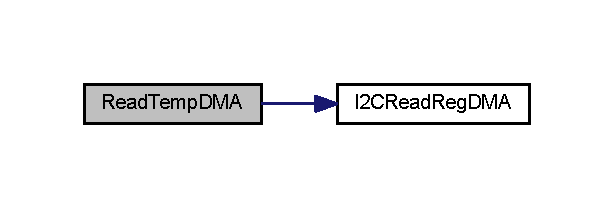
\includegraphics[width=294pt]{group___t_e_m_p_ga4a656ecef26ec3aa858327776b49d7d2_cgraph}
\end{center}
\end{figure}


\hypertarget{group___t_e_m_p_gab76473fe3a17b767072178901b184618}{\index{\-Bsp\-Temp\-: B\-S\-P Group@{\-Bsp\-Temp\-: B\-S\-P Group}!\-Read\-Temperature@{\-Read\-Temperature}}
\index{\-Read\-Temperature@{\-Read\-Temperature}!BspTemp: BSP Group@{\-Bsp\-Temp\-: B\-S\-P Group}}
\subsubsection[{\-Read\-Temperature}]{\setlength{\rightskip}{0pt plus 5cm}void {\bf \-Read\-Temperature} (
\begin{DoxyParamCaption}
\item[{{\bf \-S\-T\-R\-\_\-\-Temperture} $\ast$}]{temp}
\end{DoxyParamCaption}
)}}\label{group___t_e_m_p_gab76473fe3a17b767072178901b184618}


读取温度 


\begin{DoxyParams}[1]{\-Parameters}
 & {\em 参数名} & 参数说明 \\
\hline
\mbox{\tt in}  & {\em temp} & 温度结构体 \\
\hline
\end{DoxyParams}

\begin{DoxyRetVals}{\-Return values}
{\em 无} & \\
\hline
\end{DoxyRetVals}
\begin{DoxyParagraph}{使用全局变量 }

\end{DoxyParagraph}
\begin{DoxyNote}{\-Note}
● 执行时间\-: \par
 ● 调用周期\-: 1s \par
 ● 可否打断\-: 可以 \par

\end{DoxyNote}
\begin{DoxyParagraph}{注意\-:}
● 通过等待方式\-I2\-C读取温度, 耗时较长, 2.\-0版本以上不再使用 \par
 
\end{DoxyParagraph}


\-Here is the call graph for this function\-:\nopagebreak
\begin{figure}[H]
\begin{center}
\leavevmode
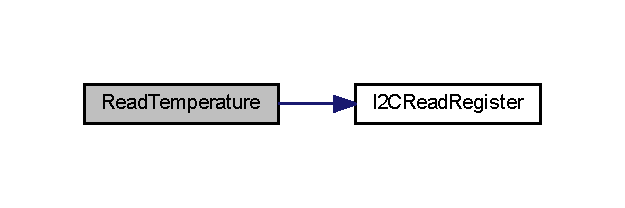
\includegraphics[width=300pt]{group___t_e_m_p_gab76473fe3a17b767072178901b184618_cgraph}
\end{center}
\end{figure}


\hypertarget{group___t_e_m_p_ga57159917434e76ddd7c731318a358dd6}{\index{\-Bsp\-Temp\-: B\-S\-P Group@{\-Bsp\-Temp\-: B\-S\-P Group}!\-Temp\-Init@{\-Temp\-Init}}
\index{\-Temp\-Init@{\-Temp\-Init}!BspTemp: BSP Group@{\-Bsp\-Temp\-: B\-S\-P Group}}
\subsubsection[{\-Temp\-Init}]{\setlength{\rightskip}{0pt plus 5cm}void {\bf \-Temp\-Init} (
\begin{DoxyParamCaption}
\item[{void}]{}
\end{DoxyParamCaption}
)}}\label{group___t_e_m_p_ga57159917434e76ddd7c731318a358dd6}


温度传感器初始化函数 

初始化温度传感器


\begin{DoxyParams}{\-Parameters}
{\em 参数名} & 参数说明 \\
\hline
{\em 无} & \\
\hline
\end{DoxyParams}

\begin{DoxyRetVals}{\-Return values}
{\em 无} & \\
\hline
\end{DoxyRetVals}
\begin{DoxyParagraph}{使用全局变量 }

\end{DoxyParagraph}
\begin{DoxyNote}{\-Note}
● 执行时间\-: \par
 ● 调用周期\-: 触发调用, 初始化时调用 \par
 ● 可否打断\-: 可以 \par

\end{DoxyNote}
\begin{DoxyParagraph}{注意\-:}
● 无 \par
 
\end{DoxyParagraph}


\-Here is the call graph for this function\-:\nopagebreak
\begin{figure}[H]
\begin{center}
\leavevmode
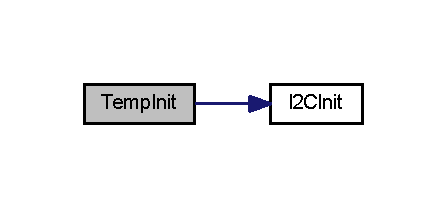
\includegraphics[width=214pt]{group___t_e_m_p_ga57159917434e76ddd7c731318a358dd6_cgraph}
\end{center}
\end{figure}




\-Here is the caller graph for this function\-:\nopagebreak
\begin{figure}[H]
\begin{center}
\leavevmode
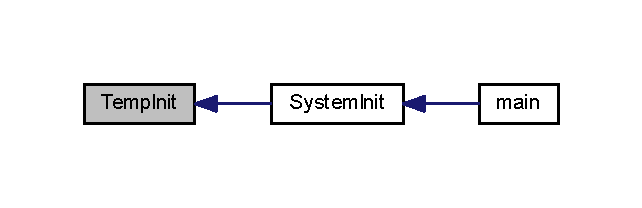
\includegraphics[width=308pt]{group___t_e_m_p_ga57159917434e76ddd7c731318a358dd6_icgraph}
\end{center}
\end{figure}



\hypertarget{group___t_i_m_e_r}{\section{\-Bsp\-Timer\-: \-B\-S\-P \-Group}
\label{group___t_i_m_e_r}\index{\-Bsp\-Timer\-: B\-S\-P Group@{\-Bsp\-Timer\-: B\-S\-P Group}}
}
\subsection*{\-Defines}
\begin{DoxyCompactItemize}
\item 
\hypertarget{group___t_i_m_e_r_gaad1f42280cb1e57ac9a12ceb897ab7f5}{\#define \hyperlink{group___t_i_m_e_r_gaad1f42280cb1e57ac9a12ceb897ab7f5}{\-T\-I\-M\-\_\-\-N\-V\-I\-C\-\_\-\-P\-R\-I\-O}~0;}\label{group___t_i_m_e_r_gaad1f42280cb1e57ac9a12ceb897ab7f5}

\begin{DoxyCompactList}\small\item\em 定时器中断优先级 \end{DoxyCompactList}\end{DoxyCompactItemize}
\subsection*{\-Functions}
\begin{DoxyCompactItemize}
\item 
void \hyperlink{group___t_i_m_e_r_ga5499adb17edb227885abaccd47631df4}{\-Timer\-Init} (void)
\begin{DoxyCompactList}\small\item\em 定时器初始化函数 \end{DoxyCompactList}\item 
void \hyperlink{group___t_i_m_e_r_ga38ad4725462bdc5e86c4ead4f04b9fc2}{\-T\-I\-M2\-\_\-\-I\-R\-Q\-Handler} (void)
\begin{DoxyCompactList}\small\item\em \-T\-I\-M2中断处理函数 \end{DoxyCompactList}\end{DoxyCompactItemize}
\subsection*{\-Variables}
\begin{DoxyCompactItemize}
\item 
\hypertarget{group___t_i_m_e_r_gabc3d26a66e3f9233e767ad6eb4dc4815}{\hyperlink{group___b_s_p_gaed742c436da53c1080638ce6ef7d13de}{u8} \hyperlink{group___t_i_m_e_r_gabc3d26a66e3f9233e767ad6eb4dc4815}{\-Req\-Heart\-Beat} = 0}\label{group___t_i_m_e_r_gabc3d26a66e3f9233e767ad6eb4dc4815}

\begin{DoxyCompactList}\small\item\em 1ms心跳定时标志位 \end{DoxyCompactList}\item 
\hypertarget{group___t_i_m_e_r_ga37b5776c7314d248dc743707d809e454}{unsigned char \hyperlink{group___t_i_m_e_r_ga37b5776c7314d248dc743707d809e454}{\-Req\-Heart\-Beat}}\label{group___t_i_m_e_r_ga37b5776c7314d248dc743707d809e454}

\begin{DoxyCompactList}\small\item\em 1ms心跳定时标志位 \end{DoxyCompactList}\end{DoxyCompactItemize}


\subsection{\-Function \-Documentation}
\hypertarget{group___t_i_m_e_r_ga38ad4725462bdc5e86c4ead4f04b9fc2}{\index{\-Bsp\-Timer\-: B\-S\-P Group@{\-Bsp\-Timer\-: B\-S\-P Group}!\-T\-I\-M2\-\_\-\-I\-R\-Q\-Handler@{\-T\-I\-M2\-\_\-\-I\-R\-Q\-Handler}}
\index{\-T\-I\-M2\-\_\-\-I\-R\-Q\-Handler@{\-T\-I\-M2\-\_\-\-I\-R\-Q\-Handler}!BspTimer: BSP Group@{\-Bsp\-Timer\-: B\-S\-P Group}}
\subsubsection[{\-T\-I\-M2\-\_\-\-I\-R\-Q\-Handler}]{\setlength{\rightskip}{0pt plus 5cm}void {\bf \-T\-I\-M2\-\_\-\-I\-R\-Q\-Handler} (
\begin{DoxyParamCaption}
\item[{void}]{}
\end{DoxyParamCaption}
)}}\label{group___t_i_m_e_r_ga38ad4725462bdc5e86c4ead4f04b9fc2}


\-T\-I\-M2中断处理函数 


\begin{DoxyParams}{\-Parameters}
{\em 参数名} & 参数说明 \\
\hline
{\em 无} & \\
\hline
\end{DoxyParams}

\begin{DoxyRetVals}{\-Return values}
{\em 无} & \\
\hline
\end{DoxyRetVals}
\begin{DoxyParagraph}{使用全局变量 }

\end{DoxyParagraph}
\begin{DoxyNote}{\-Note}
● 执行时间\-: \par
 ● 调用周期\-: 1ms, \-T\-I\-M2中断时调用 \par
 ● 可否打断\-: 可以 \par

\end{DoxyNote}
\begin{DoxyParagraph}{注意\-:}
● 无 \par
 
\end{DoxyParagraph}
\hypertarget{group___t_i_m_e_r_ga5499adb17edb227885abaccd47631df4}{\index{\-Bsp\-Timer\-: B\-S\-P Group@{\-Bsp\-Timer\-: B\-S\-P Group}!\-Timer\-Init@{\-Timer\-Init}}
\index{\-Timer\-Init@{\-Timer\-Init}!BspTimer: BSP Group@{\-Bsp\-Timer\-: B\-S\-P Group}}
\subsubsection[{\-Timer\-Init}]{\setlength{\rightskip}{0pt plus 5cm}void {\bf \-Timer\-Init} (
\begin{DoxyParamCaption}
\item[{void}]{}
\end{DoxyParamCaption}
)}}\label{group___t_i_m_e_r_ga5499adb17edb227885abaccd47631df4}


定时器初始化函数 


\begin{DoxyParams}{\-Parameters}
{\em 参数名} & 参数说明 \\
\hline
{\em 无} & \\
\hline
\end{DoxyParams}

\begin{DoxyRetVals}{\-Return values}
{\em 无} & \\
\hline
\end{DoxyRetVals}
\begin{DoxyParagraph}{使用全局变量 }

\end{DoxyParagraph}
\begin{DoxyNote}{\-Note}
● 执行时间\-: \par
 ● 调用周期\-: 触发调用, 初始化时调用 \par
 ● 可否打断\-: 可以 \par

\end{DoxyNote}
\begin{DoxyParagraph}{注意\-:}
● 无 \par
 
\end{DoxyParagraph}


\-Here is the caller graph for this function\-:\nopagebreak
\begin{figure}[H]
\begin{center}
\leavevmode
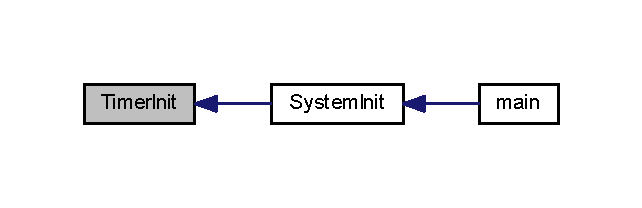
\includegraphics[width=308pt]{group___t_i_m_e_r_ga5499adb17edb227885abaccd47631df4_icgraph}
\end{center}
\end{figure}



\hypertarget{group___a_d_c}{\section{stm32\-\_\-adc\-: \-C\-P\-U \-Group}
\label{group___a_d_c}\index{stm32\-\_\-adc\-: C\-P\-U Group@{stm32\-\_\-adc\-: C\-P\-U Group}}
}
\subsection*{\-Defines}
\begin{DoxyCompactItemize}
\item 
\hypertarget{group___a_d_c_gaa594cbd44be0c5885a36c06805aefa0e}{\#define \hyperlink{group___a_d_c_gaa594cbd44be0c5885a36c06805aefa0e}{\-A\-D\-C1\-\_\-\-D\-R\-\_\-\-Address}~((\hyperlink{group___b_s_p_ga10e94b422ef0c20dcdec20d31a1f5049}{u32})0x4001244\-C)}\label{group___a_d_c_gaa594cbd44be0c5885a36c06805aefa0e}

\begin{DoxyCompactList}\small\item\em \-A\-D\-C1结果寄存器地址 \end{DoxyCompactList}\end{DoxyCompactItemize}
\subsection*{\-Functions}
\begin{DoxyCompactItemize}
\item 
\hyperlink{group___b_s_p_ga9e6c91d77e24643b888dbd1a1a590054}{u16} \hyperlink{group___a_d_c_gacb456636a61c9e02bc860319fa06f64e}{\-Get\-Adc\-Val} (void)
\begin{DoxyCompactList}\small\item\em 读取\-A\-D\-C采样值 \end{DoxyCompactList}\item 
void \hyperlink{group___a_d_c_ga39150f192703c8fc5f1885bc21deee7f}{\-A\-D\-C\-Init} (void)
\begin{DoxyCompactList}\small\item\em \-A\-D\-C初始化函数 \end{DoxyCompactList}\end{DoxyCompactItemize}


\subsection{\-Function \-Documentation}
\hypertarget{group___a_d_c_ga39150f192703c8fc5f1885bc21deee7f}{\index{stm32\-\_\-adc\-: C\-P\-U Group@{stm32\-\_\-adc\-: C\-P\-U Group}!\-A\-D\-C\-Init@{\-A\-D\-C\-Init}}
\index{\-A\-D\-C\-Init@{\-A\-D\-C\-Init}!stm32_adc: CPU Group@{stm32\-\_\-adc\-: C\-P\-U Group}}
\subsubsection[{\-A\-D\-C\-Init}]{\setlength{\rightskip}{0pt plus 5cm}void {\bf \-A\-D\-C\-Init} (
\begin{DoxyParamCaption}
\item[{void}]{}
\end{DoxyParamCaption}
)}}\label{group___a_d_c_ga39150f192703c8fc5f1885bc21deee7f}


\-A\-D\-C初始化函数 


\begin{DoxyParams}{\-Parameters}
{\em 参数名} & 参数说明 \\
\hline
{\em 无} & \\
\hline
\end{DoxyParams}

\begin{DoxyRetVals}{\-Return values}
{\em 无} & \\
\hline
\end{DoxyRetVals}
\begin{DoxyParagraph}{使用全局变量 }

\end{DoxyParagraph}
\begin{DoxyNote}{\-Note}
● 执行时间\-: \par
 ● 调用周期\-: 触发调用, 初始化时调用 \par
 ● 可否打断\-: 可以 \par

\end{DoxyNote}
\begin{DoxyParagraph}{注意\-:}
● 无 \par
 
\end{DoxyParagraph}


\-Here is the caller graph for this function\-:\nopagebreak
\begin{figure}[H]
\begin{center}
\leavevmode
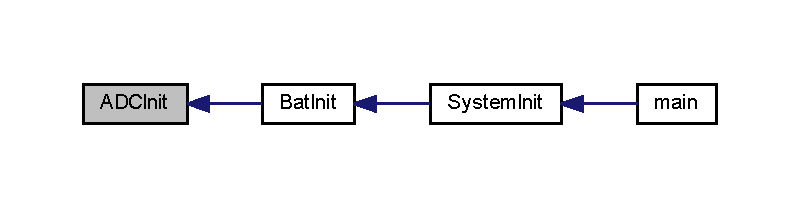
\includegraphics[width=350pt]{group___a_d_c_ga39150f192703c8fc5f1885bc21deee7f_icgraph}
\end{center}
\end{figure}


\hypertarget{group___a_d_c_gacb456636a61c9e02bc860319fa06f64e}{\index{stm32\-\_\-adc\-: C\-P\-U Group@{stm32\-\_\-adc\-: C\-P\-U Group}!\-Get\-Adc\-Val@{\-Get\-Adc\-Val}}
\index{\-Get\-Adc\-Val@{\-Get\-Adc\-Val}!stm32_adc: CPU Group@{stm32\-\_\-adc\-: C\-P\-U Group}}
\subsubsection[{\-Get\-Adc\-Val}]{\setlength{\rightskip}{0pt plus 5cm}{\bf u16} {\bf \-Get\-Adc\-Val} (
\begin{DoxyParamCaption}
\item[{void}]{}
\end{DoxyParamCaption}
)}}\label{group___a_d_c_gacb456636a61c9e02bc860319fa06f64e}


读取\-A\-D\-C采样值 


\begin{DoxyParams}{\-Parameters}
{\em 参数名} & 参数说明 \\
\hline
{\em 无} & \\
\hline
\end{DoxyParams}

\begin{DoxyRetVals}{\-Return values}
{\em \-A\-D\-C采样值} & 0$\sim$4096 \\
\hline
\end{DoxyRetVals}
\begin{DoxyParagraph}{使用全局变量 }

\end{DoxyParagraph}
\begin{DoxyNote}{\-Note}
● 执行时间\-: \par
 ● 调用周期\-: 触发调用 \par
 ● 可否打断\-: 可以 \par

\end{DoxyNote}
\begin{DoxyParagraph}{注意\-:}
● 无 \par
 
\end{DoxyParagraph}


\-Here is the caller graph for this function\-:\nopagebreak
\begin{figure}[H]
\begin{center}
\leavevmode
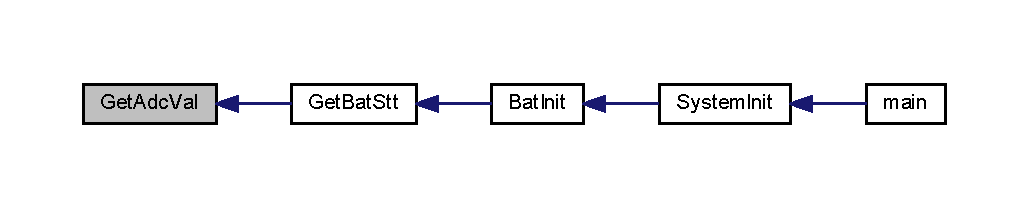
\includegraphics[width=350pt]{group___a_d_c_gacb456636a61c9e02bc860319fa06f64e_icgraph}
\end{center}
\end{figure}



\hypertarget{group___i2_c}{\section{stm32\-\_\-i2c\-: \-C\-P\-U \-Group}
\label{group___i2_c}\index{stm32\-\_\-i2c\-: C\-P\-U Group@{stm32\-\_\-i2c\-: C\-P\-U Group}}
}
\subsection*{\-Data \-Structures}
\begin{DoxyCompactItemize}
\item 
struct \hyperlink{struct_s_t_r___i2c_proc}{\-S\-T\-R\-\_\-\-I2c\-Proc}
\begin{DoxyCompactList}\small\item\em \-I2\-C收发过程相关中间变量结构体 \end{DoxyCompactList}\item 
struct \hyperlink{struct_s_t_r___i2_c}{\-S\-T\-R\-\_\-\-I2\-C}
\begin{DoxyCompactList}\small\item\em \-I2\-C收发结构体 \end{DoxyCompactList}\end{DoxyCompactItemize}
\subsection*{\-Defines}
\begin{DoxyCompactItemize}
\item 
\hypertarget{group___i2_c_gabf2bd419e88218ef9ad3a3a7dd2b145c}{\#define \hyperlink{group___i2_c_gabf2bd419e88218ef9ad3a3a7dd2b145c}{\-I2\-C1\-\_\-\-D\-R\-\_\-\-Address}~0x40005410}\label{group___i2_c_gabf2bd419e88218ef9ad3a3a7dd2b145c}

\begin{DoxyCompactList}\small\item\em \-I2\-C1数据寄存器地址 \end{DoxyCompactList}\item 
\hypertarget{group___i2_c_gacb13e35c5e812ea51d29e833be1b72be}{\#define \hyperlink{group___i2_c_gacb13e35c5e812ea51d29e833be1b72be}{\-I2\-C\-\_\-\-R\-D}~0}\label{group___i2_c_gacb13e35c5e812ea51d29e833be1b72be}

\begin{DoxyCompactList}\small\item\em 读寄存器 \end{DoxyCompactList}\item 
\hypertarget{group___i2_c_ga5a3e7b03fa275ec2d334e95a2caf6477}{\#define \hyperlink{group___i2_c_ga5a3e7b03fa275ec2d334e95a2caf6477}{\-I2\-C\-\_\-\-W\-R}~1}\label{group___i2_c_ga5a3e7b03fa275ec2d334e95a2caf6477}

\begin{DoxyCompactList}\small\item\em 写寄存器 \end{DoxyCompactList}\item 
\hypertarget{group___i2_c_ga7c7e0c31bae2ea1fef32d39d61c61166}{\#define \hyperlink{group___i2_c_ga7c7e0c31bae2ea1fef32d39d61c61166}{\-T\-I\-M\-E\-O\-U\-T\-I2\-C}~5000}\label{group___i2_c_ga7c7e0c31bae2ea1fef32d39d61c61166}

\begin{DoxyCompactList}\small\item\em i2c超时时间 \end{DoxyCompactList}\end{DoxyCompactItemize}
\subsection*{\-Typedefs}
\begin{DoxyCompactItemize}
\item 
\hypertarget{group___i2_c_gaed499a25832ba009a4a212e310ddac45}{typedef enum \hyperlink{group___i2_c_ga3acd3f8324118cb8c44f79b0fa24190a}{i2c\-\_\-state} \hyperlink{group___i2_c_gaed499a25832ba009a4a212e310ddac45}{\-I2\-C\-\_\-\-S\-T\-A\-T\-E}}\label{group___i2_c_gaed499a25832ba009a4a212e310ddac45}

\begin{DoxyCompactList}\small\item\em \-I2\-C收发过程状态 \end{DoxyCompactList}\end{DoxyCompactItemize}
\subsection*{\-Enumerations}
\begin{DoxyCompactItemize}
\item 
enum \hyperlink{group___i2_c_ga3acd3f8324118cb8c44f79b0fa24190a}{i2c\-\_\-state} \{ \*
\hyperlink{group___i2_c_gga3acd3f8324118cb8c44f79b0fa24190aa775c023b24ee56b90ca660f91522b78a}{\-C\-O\-M\-M\-\_\-\-D\-O\-N\-E} =  0, 
\hyperlink{group___i2_c_gga3acd3f8324118cb8c44f79b0fa24190aa671d1da07d0d895d5fdc1897b059bdc3}{\-C\-O\-M\-M\-\_\-\-P\-R\-E} =  1, 
{\bfseries \-C\-O\-M\-M\-\_\-\-I\-N\-\_\-\-P\-R\-O\-C\-E\-S\-S} =  2, 
{\bfseries \-C\-H\-E\-C\-K\-\_\-\-I\-N\-\_\-\-P\-R\-O\-C\-E\-S\-S} =  3, 
\*
\hyperlink{group___i2_c_gga3acd3f8324118cb8c44f79b0fa24190aa4a81f9df06f1e648593f415eba9eb1d0}{\-C\-O\-M\-M\-\_\-\-E\-X\-I\-T} =  4
 \}
\begin{DoxyCompactList}\small\item\em \-I2\-C收发过程状态 \end{DoxyCompactList}\end{DoxyCompactItemize}
\subsection*{\-Functions}
\begin{DoxyCompactItemize}
\item 
\hyperlink{group___b_s_p_gaed742c436da53c1080638ce6ef7d13de}{u8} \hyperlink{group___i2_c_ga03d622963958101e7a276a3188365c21}{\-I2\-C\-Read\-Register} (\hyperlink{group___b_s_p_gaed742c436da53c1080638ce6ef7d13de}{u8} slave\-Address, \hyperlink{group___b_s_p_gaed742c436da53c1080638ce6ef7d13de}{u8} register\-Address, \hyperlink{group___b_s_p_gaed742c436da53c1080638ce6ef7d13de}{u8} $\ast$buf, \hyperlink{group___b_s_p_gaed742c436da53c1080638ce6ef7d13de}{u8} num)
\begin{DoxyCompactList}\small\item\em 读取i2c设备的寄存器 \end{DoxyCompactList}\item 
\hyperlink{group___b_s_p_gaed742c436da53c1080638ce6ef7d13de}{u8} \hyperlink{group___i2_c_gae595c5041521bcb3d1d19a2d97bdf365}{\-I2\-C\-Write\-Register} (\hyperlink{group___b_s_p_gaed742c436da53c1080638ce6ef7d13de}{u8} slave\-Address, \hyperlink{group___b_s_p_gaed742c436da53c1080638ce6ef7d13de}{u8} register\-Address, \hyperlink{group___b_s_p_gaed742c436da53c1080638ce6ef7d13de}{u8} $\ast$buf, \hyperlink{group___b_s_p_gaed742c436da53c1080638ce6ef7d13de}{u8} num)
\begin{DoxyCompactList}\small\item\em 写i2c设备的寄存器 \end{DoxyCompactList}\item 
void \hyperlink{group___i2_c_ga7d23473bd5eb72909c1a3588a70bb237}{\-I2\-C\-Init} (void)
\begin{DoxyCompactList}\small\item\em i2c控制器初始化函数 \end{DoxyCompactList}\item 
void \hyperlink{group___i2_c_ga8d90041eb72157c18ceaf840e22945a3}{\-I2\-C\-Read\-Reg\-D\-M\-A} (\hyperlink{group___b_s_p_gaed742c436da53c1080638ce6ef7d13de}{u8} slave\-Addr, \hyperlink{group___b_s_p_gaed742c436da53c1080638ce6ef7d13de}{u8} reg\-Addr, \hyperlink{group___b_s_p_gaed742c436da53c1080638ce6ef7d13de}{u8} $\ast$buf, \hyperlink{group___b_s_p_gaed742c436da53c1080638ce6ef7d13de}{u8} num)
\begin{DoxyCompactList}\small\item\em \-D\-M\-A方式读取i2c设备的寄存器 \end{DoxyCompactList}\item 
void \hyperlink{group___i2_c_ga5ecce9ad43038ccd3847f2f9b90bbc36}{\-I2\-C\-Write\-Reg\-D\-M\-A} (\hyperlink{group___b_s_p_gaed742c436da53c1080638ce6ef7d13de}{u8} slave\-Addr, \hyperlink{group___b_s_p_gaed742c436da53c1080638ce6ef7d13de}{u8} reg\-Addr, \hyperlink{group___b_s_p_gaed742c436da53c1080638ce6ef7d13de}{u8} $\ast$buf, \hyperlink{group___b_s_p_gaed742c436da53c1080638ce6ef7d13de}{u8} num)
\begin{DoxyCompactList}\small\item\em \-D\-M\-A方式写i2c设备的寄存器 \end{DoxyCompactList}\item 
void \hyperlink{group___i2_c_ga272ffa65eb8ff5c4a065b0d3473611cd}{\-I2\-C1\-\_\-\-E\-V\-\_\-\-I\-R\-Q\-Handler} (void)
\begin{DoxyCompactList}\small\item\em \-I2\-C1事件中断处理函数 \end{DoxyCompactList}\item 
void \hyperlink{group___i2_c_gad25274aece51e7f5b821f5d32b31bddf}{\-I2\-C1\-\_\-\-E\-R\-\_\-\-I\-R\-Q\-Handler} (void)
\begin{DoxyCompactList}\small\item\em \-I2\-C1错误中断处理函数 \end{DoxyCompactList}\item 
void \hyperlink{group___i2_c_gab74311855aee10304ffc57c319c91ed3}{\-D\-M\-A1\-\_\-\-Channel6\-\_\-\-I\-R\-Q\-Handler} (void)
\begin{DoxyCompactList}\small\item\em \-D\-M\-A1\-\_\-\-C\-H6中断处理函数 \end{DoxyCompactList}\item 
void \hyperlink{group___i2_c_ga7a964205d5b1ce4b9c69ae6a105145ca}{\-D\-M\-A1\-\_\-\-Channel7\-\_\-\-I\-R\-Q\-Handler} (void)
\begin{DoxyCompactList}\small\item\em \-D\-M\-A1\-\_\-\-C\-H7中断处理函数 \end{DoxyCompactList}\end{DoxyCompactItemize}
\subsection*{\-Variables}
\begin{DoxyCompactItemize}
\item 
\hypertarget{group___i2_c_ga74d3522c7f760f53f9a042059dae0488}{\hyperlink{struct_s_t_r___i2_c}{\-S\-T\-R\-\_\-\-I2\-C} \hyperlink{group___i2_c_ga74d3522c7f760f53f9a042059dae0488}{\-I2c} = \{0,\}}\label{group___i2_c_ga74d3522c7f760f53f9a042059dae0488}

\begin{DoxyCompactList}\small\item\em \-I2\-C收发结构体 \end{DoxyCompactList}\item 
\hypertarget{group___i2_c_ga74d3522c7f760f53f9a042059dae0488}{\hyperlink{struct_s_t_r___i2_c}{\-S\-T\-R\-\_\-\-I2\-C} \hyperlink{group___i2_c_ga74d3522c7f760f53f9a042059dae0488}{\-I2c}}\label{group___i2_c_ga74d3522c7f760f53f9a042059dae0488}

\begin{DoxyCompactList}\small\item\em \-I2\-C收发结构体 \end{DoxyCompactList}\end{DoxyCompactItemize}


\subsection{\-Enumeration \-Type \-Documentation}
\hypertarget{group___i2_c_ga3acd3f8324118cb8c44f79b0fa24190a}{\index{stm32\-\_\-i2c\-: C\-P\-U Group@{stm32\-\_\-i2c\-: C\-P\-U Group}!i2c\-\_\-state@{i2c\-\_\-state}}
\index{i2c\-\_\-state@{i2c\-\_\-state}!stm32_i2c: CPU Group@{stm32\-\_\-i2c\-: C\-P\-U Group}}
\subsubsection[{i2c\-\_\-state}]{\setlength{\rightskip}{0pt plus 5cm}enum {\bf i2c\-\_\-state}}}\label{group___i2_c_ga3acd3f8324118cb8c44f79b0fa24190a}


\-I2\-C收发过程状态 

\begin{Desc}
\item[\-Enumerator\-: ]\par
\begin{description}
\index{\-C\-O\-M\-M\-\_\-\-D\-O\-N\-E@{\-C\-O\-M\-M\-\_\-\-D\-O\-N\-E}!stm32\-\_\-i2c\-: C\-P\-U Group@{stm32\-\_\-i2c\-: C\-P\-U Group}}\index{stm32\-\_\-i2c\-: C\-P\-U Group@{stm32\-\_\-i2c\-: C\-P\-U Group}!\-C\-O\-M\-M\-\_\-\-D\-O\-N\-E@{\-C\-O\-M\-M\-\_\-\-D\-O\-N\-E}}\item[{\em 
\hypertarget{group___i2_c_gga3acd3f8324118cb8c44f79b0fa24190aa775c023b24ee56b90ca660f91522b78a}{\-C\-O\-M\-M\-\_\-\-D\-O\-N\-E}\label{group___i2_c_gga3acd3f8324118cb8c44f79b0fa24190aa775c023b24ee56b90ca660f91522b78a}
}]成功 \index{\-C\-O\-M\-M\-\_\-\-P\-R\-E@{\-C\-O\-M\-M\-\_\-\-P\-R\-E}!stm32\-\_\-i2c\-: C\-P\-U Group@{stm32\-\_\-i2c\-: C\-P\-U Group}}\index{stm32\-\_\-i2c\-: C\-P\-U Group@{stm32\-\_\-i2c\-: C\-P\-U Group}!\-C\-O\-M\-M\-\_\-\-P\-R\-E@{\-C\-O\-M\-M\-\_\-\-P\-R\-E}}\item[{\em 
\hypertarget{group___i2_c_gga3acd3f8324118cb8c44f79b0fa24190aa671d1da07d0d895d5fdc1897b059bdc3}{\-C\-O\-M\-M\-\_\-\-P\-R\-E}\label{group___i2_c_gga3acd3f8324118cb8c44f79b0fa24190aa671d1da07d0d895d5fdc1897b059bdc3}
}]准备 \index{\-C\-O\-M\-M\-\_\-\-E\-X\-I\-T@{\-C\-O\-M\-M\-\_\-\-E\-X\-I\-T}!stm32\-\_\-i2c\-: C\-P\-U Group@{stm32\-\_\-i2c\-: C\-P\-U Group}}\index{stm32\-\_\-i2c\-: C\-P\-U Group@{stm32\-\_\-i2c\-: C\-P\-U Group}!\-C\-O\-M\-M\-\_\-\-E\-X\-I\-T@{\-C\-O\-M\-M\-\_\-\-E\-X\-I\-T}}\item[{\em 
\hypertarget{group___i2_c_gga3acd3f8324118cb8c44f79b0fa24190aa4a81f9df06f1e648593f415eba9eb1d0}{\-C\-O\-M\-M\-\_\-\-E\-X\-I\-T}\label{group___i2_c_gga3acd3f8324118cb8c44f79b0fa24190aa4a81f9df06f1e648593f415eba9eb1d0}
}]失败退出 \end{description}
\end{Desc}



\subsection{\-Function \-Documentation}
\hypertarget{group___i2_c_gab74311855aee10304ffc57c319c91ed3}{\index{stm32\-\_\-i2c\-: C\-P\-U Group@{stm32\-\_\-i2c\-: C\-P\-U Group}!\-D\-M\-A1\-\_\-\-Channel6\-\_\-\-I\-R\-Q\-Handler@{\-D\-M\-A1\-\_\-\-Channel6\-\_\-\-I\-R\-Q\-Handler}}
\index{\-D\-M\-A1\-\_\-\-Channel6\-\_\-\-I\-R\-Q\-Handler@{\-D\-M\-A1\-\_\-\-Channel6\-\_\-\-I\-R\-Q\-Handler}!stm32_i2c: CPU Group@{stm32\-\_\-i2c\-: C\-P\-U Group}}
\subsubsection[{\-D\-M\-A1\-\_\-\-Channel6\-\_\-\-I\-R\-Q\-Handler}]{\setlength{\rightskip}{0pt plus 5cm}void {\bf \-D\-M\-A1\-\_\-\-Channel6\-\_\-\-I\-R\-Q\-Handler} (
\begin{DoxyParamCaption}
\item[{void}]{}
\end{DoxyParamCaption}
)}}\label{group___i2_c_gab74311855aee10304ffc57c319c91ed3}


\-D\-M\-A1\-\_\-\-C\-H6中断处理函数 


\begin{DoxyParams}{\-Parameters}
{\em 参数名} & 参数说明 \\
\hline
{\em 无} & \\
\hline
\end{DoxyParams}

\begin{DoxyRetVals}{\-Return values}
{\em 无} & \\
\hline
\end{DoxyRetVals}
\begin{DoxyParagraph}{使用全局变量 }

\end{DoxyParagraph}
\begin{DoxyNote}{\-Note}
● 执行时间\-: \par
 ● 调用周期\-: i2c1发送完成后,\-D\-M\-A1\-\_\-\-C\-H6传输完成中断时调用 \par
 ● 可否打断\-: 可以 \par

\end{DoxyNote}
\begin{DoxyParagraph}{注意\-:}
● 无 \par
 
\end{DoxyParagraph}
\hypertarget{group___i2_c_ga7a964205d5b1ce4b9c69ae6a105145ca}{\index{stm32\-\_\-i2c\-: C\-P\-U Group@{stm32\-\_\-i2c\-: C\-P\-U Group}!\-D\-M\-A1\-\_\-\-Channel7\-\_\-\-I\-R\-Q\-Handler@{\-D\-M\-A1\-\_\-\-Channel7\-\_\-\-I\-R\-Q\-Handler}}
\index{\-D\-M\-A1\-\_\-\-Channel7\-\_\-\-I\-R\-Q\-Handler@{\-D\-M\-A1\-\_\-\-Channel7\-\_\-\-I\-R\-Q\-Handler}!stm32_i2c: CPU Group@{stm32\-\_\-i2c\-: C\-P\-U Group}}
\subsubsection[{\-D\-M\-A1\-\_\-\-Channel7\-\_\-\-I\-R\-Q\-Handler}]{\setlength{\rightskip}{0pt plus 5cm}void {\bf \-D\-M\-A1\-\_\-\-Channel7\-\_\-\-I\-R\-Q\-Handler} (
\begin{DoxyParamCaption}
\item[{void}]{}
\end{DoxyParamCaption}
)}}\label{group___i2_c_ga7a964205d5b1ce4b9c69ae6a105145ca}


\-D\-M\-A1\-\_\-\-C\-H7中断处理函数 


\begin{DoxyParams}{\-Parameters}
{\em 参数名} & 参数说明 \\
\hline
{\em 无} & \\
\hline
\end{DoxyParams}

\begin{DoxyRetVals}{\-Return values}
{\em 无} & \\
\hline
\end{DoxyRetVals}
\begin{DoxyParagraph}{使用全局变量 }

\end{DoxyParagraph}
\begin{DoxyNote}{\-Note}
● 执行时间\-: \par
 ● 调用周期\-: i2c1接收完成后,\-D\-M\-A1\-\_\-\-C\-H7传输完成中断时调用 \par
 ● 可否打断\-: 可以 \par

\end{DoxyNote}
\begin{DoxyParagraph}{注意\-:}
● 无 \par
 
\end{DoxyParagraph}
\hypertarget{group___i2_c_gad25274aece51e7f5b821f5d32b31bddf}{\index{stm32\-\_\-i2c\-: C\-P\-U Group@{stm32\-\_\-i2c\-: C\-P\-U Group}!\-I2\-C1\-\_\-\-E\-R\-\_\-\-I\-R\-Q\-Handler@{\-I2\-C1\-\_\-\-E\-R\-\_\-\-I\-R\-Q\-Handler}}
\index{\-I2\-C1\-\_\-\-E\-R\-\_\-\-I\-R\-Q\-Handler@{\-I2\-C1\-\_\-\-E\-R\-\_\-\-I\-R\-Q\-Handler}!stm32_i2c: CPU Group@{stm32\-\_\-i2c\-: C\-P\-U Group}}
\subsubsection[{\-I2\-C1\-\_\-\-E\-R\-\_\-\-I\-R\-Q\-Handler}]{\setlength{\rightskip}{0pt plus 5cm}void {\bf \-I2\-C1\-\_\-\-E\-R\-\_\-\-I\-R\-Q\-Handler} (
\begin{DoxyParamCaption}
\item[{void}]{}
\end{DoxyParamCaption}
)}}\label{group___i2_c_gad25274aece51e7f5b821f5d32b31bddf}


\-I2\-C1错误中断处理函数 


\begin{DoxyParams}{\-Parameters}
{\em 参数名} & 参数说明 \\
\hline
{\em 无} & \\
\hline
\end{DoxyParams}

\begin{DoxyRetVals}{\-Return values}
{\em 无} & \\
\hline
\end{DoxyRetVals}
\begin{DoxyParagraph}{使用全局变量 }

\end{DoxyParagraph}
\begin{DoxyNote}{\-Note}
● 执行时间\-: \par
 ● 调用周期\-: \-I2\-C1发生错误时调用 \par
 ● 可否打断\-: 可以 \par

\end{DoxyNote}
\begin{DoxyParagraph}{注意\-:}
● 无 \par
 
\end{DoxyParagraph}
\hypertarget{group___i2_c_ga272ffa65eb8ff5c4a065b0d3473611cd}{\index{stm32\-\_\-i2c\-: C\-P\-U Group@{stm32\-\_\-i2c\-: C\-P\-U Group}!\-I2\-C1\-\_\-\-E\-V\-\_\-\-I\-R\-Q\-Handler@{\-I2\-C1\-\_\-\-E\-V\-\_\-\-I\-R\-Q\-Handler}}
\index{\-I2\-C1\-\_\-\-E\-V\-\_\-\-I\-R\-Q\-Handler@{\-I2\-C1\-\_\-\-E\-V\-\_\-\-I\-R\-Q\-Handler}!stm32_i2c: CPU Group@{stm32\-\_\-i2c\-: C\-P\-U Group}}
\subsubsection[{\-I2\-C1\-\_\-\-E\-V\-\_\-\-I\-R\-Q\-Handler}]{\setlength{\rightskip}{0pt plus 5cm}void {\bf \-I2\-C1\-\_\-\-E\-V\-\_\-\-I\-R\-Q\-Handler} (
\begin{DoxyParamCaption}
\item[{void}]{}
\end{DoxyParamCaption}
)}}\label{group___i2_c_ga272ffa65eb8ff5c4a065b0d3473611cd}


\-I2\-C1事件中断处理函数 


\begin{DoxyParams}{\-Parameters}
{\em 参数名} & 参数说明 \\
\hline
{\em 无} & \\
\hline
\end{DoxyParams}

\begin{DoxyRetVals}{\-Return values}
{\em 无} & \\
\hline
\end{DoxyRetVals}
\begin{DoxyParagraph}{使用全局变量 }

\end{DoxyParagraph}
\begin{DoxyNote}{\-Note}
● 执行时间\-: \par
 ● 调用周期\-: \-I2\-C1状态发生变化时调用 \par
 ● 可否打断\-: 可以 \par

\end{DoxyNote}
\begin{DoxyParagraph}{注意\-:}
● 无 \par
 
\end{DoxyParagraph}
\hypertarget{group___i2_c_ga7d23473bd5eb72909c1a3588a70bb237}{\index{stm32\-\_\-i2c\-: C\-P\-U Group@{stm32\-\_\-i2c\-: C\-P\-U Group}!\-I2\-C\-Init@{\-I2\-C\-Init}}
\index{\-I2\-C\-Init@{\-I2\-C\-Init}!stm32_i2c: CPU Group@{stm32\-\_\-i2c\-: C\-P\-U Group}}
\subsubsection[{\-I2\-C\-Init}]{\setlength{\rightskip}{0pt plus 5cm}void {\bf \-I2\-C\-Init} (
\begin{DoxyParamCaption}
\item[{void}]{}
\end{DoxyParamCaption}
)}}\label{group___i2_c_ga7d23473bd5eb72909c1a3588a70bb237}


i2c控制器初始化函数 


\begin{DoxyParams}{\-Parameters}
{\em 参数名} & 参数说明 \\
\hline
{\em 无} & \\
\hline
\end{DoxyParams}

\begin{DoxyRetVals}{\-Return values}
{\em 无} & \\
\hline
\end{DoxyRetVals}
\begin{DoxyParagraph}{使用全局变量 }

\end{DoxyParagraph}
\begin{DoxyNote}{\-Note}
● 执行时间\-: \par
 ● 调用周期\-: 触发调用, 初始化时调用 \par
 ● 可否打断\-: 可以 \par

\end{DoxyNote}
\begin{DoxyParagraph}{注意\-:}
● 无 \par
 
\end{DoxyParagraph}


\-Here is the caller graph for this function\-:\nopagebreak
\begin{figure}[H]
\begin{center}
\leavevmode
\includegraphics[width=350pt]{group___i2_c_ga7d23473bd5eb72909c1a3588a70bb237_icgraph}
\end{center}
\end{figure}


\hypertarget{group___i2_c_ga8d90041eb72157c18ceaf840e22945a3}{\index{stm32\-\_\-i2c\-: C\-P\-U Group@{stm32\-\_\-i2c\-: C\-P\-U Group}!\-I2\-C\-Read\-Reg\-D\-M\-A@{\-I2\-C\-Read\-Reg\-D\-M\-A}}
\index{\-I2\-C\-Read\-Reg\-D\-M\-A@{\-I2\-C\-Read\-Reg\-D\-M\-A}!stm32_i2c: CPU Group@{stm32\-\_\-i2c\-: C\-P\-U Group}}
\subsubsection[{\-I2\-C\-Read\-Reg\-D\-M\-A}]{\setlength{\rightskip}{0pt plus 5cm}void {\bf \-I2\-C\-Read\-Reg\-D\-M\-A} (
\begin{DoxyParamCaption}
\item[{{\bf u8}}]{slave\-Addr, }
\item[{{\bf u8}}]{reg\-Addr, }
\item[{{\bf u8} $\ast$}]{buf, }
\item[{{\bf u8}}]{num}
\end{DoxyParamCaption}
)}}\label{group___i2_c_ga8d90041eb72157c18ceaf840e22945a3}


\-D\-M\-A方式读取i2c设备的寄存器 


\begin{DoxyParams}[1]{\-Parameters}
 & {\em 参数名} & 参数说明 \\
\hline
\mbox{\tt in}  & {\em slave\-Addr} & 从设备地址 \\
\hline
\mbox{\tt in}  & {\em reg\-Addr} & 寄存器地址 \\
\hline
\mbox{\tt out}  & {\em $\ast$buf} & 读取的值存放的缓存区 \\
\hline
\mbox{\tt in}  & {\em num} & 需要读取的字节数 \\
\hline
\end{DoxyParams}

\begin{DoxyRetVals}{\-Return values}
{\em 无} & \\
\hline
\end{DoxyRetVals}
\begin{DoxyParagraph}{使用全局变量 }

\end{DoxyParagraph}
\begin{DoxyNote}{\-Note}
● 执行时间\-: \par
 ● 调用周期\-: 触发调用, 初始化时调用 \par
 ● 可否打断\-: 可以 \par

\end{DoxyNote}
\begin{DoxyParagraph}{注意\-:}
● 无 \par
 
\end{DoxyParagraph}


\-Here is the caller graph for this function\-:\nopagebreak
\begin{figure}[H]
\begin{center}
\leavevmode
\includegraphics[width=294pt]{group___i2_c_ga8d90041eb72157c18ceaf840e22945a3_icgraph}
\end{center}
\end{figure}


\hypertarget{group___i2_c_ga03d622963958101e7a276a3188365c21}{\index{stm32\-\_\-i2c\-: C\-P\-U Group@{stm32\-\_\-i2c\-: C\-P\-U Group}!\-I2\-C\-Read\-Register@{\-I2\-C\-Read\-Register}}
\index{\-I2\-C\-Read\-Register@{\-I2\-C\-Read\-Register}!stm32_i2c: CPU Group@{stm32\-\_\-i2c\-: C\-P\-U Group}}
\subsubsection[{\-I2\-C\-Read\-Register}]{\setlength{\rightskip}{0pt plus 5cm}{\bf u8} {\bf \-I2\-C\-Read\-Register} (
\begin{DoxyParamCaption}
\item[{{\bf u8}}]{slave\-Address, }
\item[{{\bf u8}}]{register\-Address, }
\item[{{\bf u8} $\ast$}]{buf, }
\item[{{\bf u8}}]{num}
\end{DoxyParamCaption}
)}}\label{group___i2_c_ga03d622963958101e7a276a3188365c21}


读取i2c设备的寄存器 


\begin{DoxyParams}[1]{\-Parameters}
 & {\em 参数名} & 参数说明 \\
\hline
\mbox{\tt in}  & {\em slave\-Address} & 从设备地址 \\
\hline
\mbox{\tt in}  & {\em register\-Address} & 寄存器地址 \\
\hline
\mbox{\tt out}  & {\em $\ast$buf} & 读取的值存放的缓存区 \\
\hline
\mbox{\tt in}  & {\em num} & 需要读取的字节数 \\
\hline
\end{DoxyParams}

\begin{DoxyRetVals}{\-Return values}
{\em 0-\/失败} & 1-\/成功 \\
\hline
\end{DoxyRetVals}
\begin{DoxyParagraph}{使用全局变量 }

\end{DoxyParagraph}
\begin{DoxyNote}{\-Note}
● 执行时间\-: \par
 ● 调用周期\-: 触发调用, 初始化时调用 \par
 ● 可否打断\-: 可以 \par

\end{DoxyNote}
\begin{DoxyParagraph}{注意\-:}
● 无 \par
 
\end{DoxyParagraph}


\-Here is the caller graph for this function\-:\nopagebreak
\begin{figure}[H]
\begin{center}
\leavevmode
\includegraphics[width=350pt]{group___i2_c_ga03d622963958101e7a276a3188365c21_icgraph}
\end{center}
\end{figure}


\hypertarget{group___i2_c_ga5ecce9ad43038ccd3847f2f9b90bbc36}{\index{stm32\-\_\-i2c\-: C\-P\-U Group@{stm32\-\_\-i2c\-: C\-P\-U Group}!\-I2\-C\-Write\-Reg\-D\-M\-A@{\-I2\-C\-Write\-Reg\-D\-M\-A}}
\index{\-I2\-C\-Write\-Reg\-D\-M\-A@{\-I2\-C\-Write\-Reg\-D\-M\-A}!stm32_i2c: CPU Group@{stm32\-\_\-i2c\-: C\-P\-U Group}}
\subsubsection[{\-I2\-C\-Write\-Reg\-D\-M\-A}]{\setlength{\rightskip}{0pt plus 5cm}void {\bf \-I2\-C\-Write\-Reg\-D\-M\-A} (
\begin{DoxyParamCaption}
\item[{{\bf u8}}]{slave\-Addr, }
\item[{{\bf u8}}]{reg\-Addr, }
\item[{{\bf u8} $\ast$}]{buf, }
\item[{{\bf u8}}]{num}
\end{DoxyParamCaption}
)}}\label{group___i2_c_ga5ecce9ad43038ccd3847f2f9b90bbc36}


\-D\-M\-A方式写i2c设备的寄存器 


\begin{DoxyParams}[1]{\-Parameters}
 & {\em 参数名} & 参数说明 \\
\hline
\mbox{\tt in}  & {\em slave\-Addr} & 从设备地址 \\
\hline
\mbox{\tt in}  & {\em reg\-Addr} & 寄存器地址 \\
\hline
\mbox{\tt in}  & {\em $\ast$buf} & 写入的值存放的缓存区 \\
\hline
\mbox{\tt in}  & {\em num} & 需要读取的字节数 \\
\hline
\end{DoxyParams}

\begin{DoxyRetVals}{\-Return values}
{\em 0-\/失败} & 1-\/成功 \\
\hline
\end{DoxyRetVals}
\begin{DoxyParagraph}{使用全局变量 }

\end{DoxyParagraph}
\begin{DoxyNote}{\-Note}
● 执行时间\-: \par
 ● 调用周期\-: 触发调用, 初始化时调用 \par
 ● 可否打断\-: 可以 \par

\end{DoxyNote}
\begin{DoxyParagraph}{注意\-:}
● 无 \par
 
\end{DoxyParagraph}
\hypertarget{group___i2_c_gae595c5041521bcb3d1d19a2d97bdf365}{\index{stm32\-\_\-i2c\-: C\-P\-U Group@{stm32\-\_\-i2c\-: C\-P\-U Group}!\-I2\-C\-Write\-Register@{\-I2\-C\-Write\-Register}}
\index{\-I2\-C\-Write\-Register@{\-I2\-C\-Write\-Register}!stm32_i2c: CPU Group@{stm32\-\_\-i2c\-: C\-P\-U Group}}
\subsubsection[{\-I2\-C\-Write\-Register}]{\setlength{\rightskip}{0pt plus 5cm}{\bf u8} {\bf \-I2\-C\-Write\-Register} (
\begin{DoxyParamCaption}
\item[{{\bf u8}}]{slave\-Address, }
\item[{{\bf u8}}]{register\-Address, }
\item[{{\bf u8} $\ast$}]{buf, }
\item[{{\bf u8}}]{num}
\end{DoxyParamCaption}
)}}\label{group___i2_c_gae595c5041521bcb3d1d19a2d97bdf365}


写i2c设备的寄存器 


\begin{DoxyParams}[1]{\-Parameters}
 & {\em 参数名} & 参数说明 \\
\hline
\mbox{\tt in}  & {\em slave\-Address} & 从设备地址 \\
\hline
\mbox{\tt in}  & {\em register\-Address} & 寄存器地址 \\
\hline
\mbox{\tt in}  & {\em $\ast$buf} & 写入的值存放的缓存区 \\
\hline
\mbox{\tt in}  & {\em num} & 需要读取的字节数 \\
\hline
\end{DoxyParams}

\begin{DoxyRetVals}{\-Return values}
{\em 0-\/失败} & 1-\/成功 \\
\hline
\end{DoxyRetVals}
\begin{DoxyParagraph}{使用全局变量 }

\end{DoxyParagraph}
\begin{DoxyNote}{\-Note}
● 执行时间\-: \par
 ● 调用周期\-: 触发调用, 初始化时调用 \par
 ● 可否打断\-: 可以 \par

\end{DoxyNote}
\begin{DoxyParagraph}{注意\-:}
● 无 \par
 
\end{DoxyParagraph}


\-Here is the caller graph for this function\-:\nopagebreak
\begin{figure}[H]
\begin{center}
\leavevmode
\includegraphics[width=350pt]{group___i2_c_gae595c5041521bcb3d1d19a2d97bdf365_icgraph}
\end{center}
\end{figure}



\hypertarget{group___p_w_m}{\section{stm32\-\_\-pwm\-: \-C\-P\-U \-Group}
\label{group___p_w_m}\index{stm32\-\_\-pwm\-: C\-P\-U Group@{stm32\-\_\-pwm\-: C\-P\-U Group}}
}
\subsection*{\-Functions}
\begin{DoxyCompactItemize}
\item 
void \hyperlink{group___p_w_m_ga2a5f4a56e66fe7a6115e8042b1d9eb92}{\-Pwm\-Init} (void)
\begin{DoxyCompactList}\small\item\em \-P\-W\-M初始化函数 \end{DoxyCompactList}\item 
void \hyperlink{group___p_w_m_ga2e07f7252bebe119d8a5120fb9ef86fe}{\-Pwm\-Set} (\hyperlink{group___b_s_p_ga9e6c91d77e24643b888dbd1a1a590054}{u16} pwm\-Ch1, \hyperlink{group___b_s_p_ga9e6c91d77e24643b888dbd1a1a590054}{u16} pwm\-Ch2, \hyperlink{group___b_s_p_ga9e6c91d77e24643b888dbd1a1a590054}{u16} pwm\-Ch3)
\begin{DoxyCompactList}\small\item\em \-P\-W\-M占空比设置 \end{DoxyCompactList}\end{DoxyCompactItemize}


\subsection{\-Function \-Documentation}
\hypertarget{group___p_w_m_ga2a5f4a56e66fe7a6115e8042b1d9eb92}{\index{stm32\-\_\-pwm\-: C\-P\-U Group@{stm32\-\_\-pwm\-: C\-P\-U Group}!\-Pwm\-Init@{\-Pwm\-Init}}
\index{\-Pwm\-Init@{\-Pwm\-Init}!stm32_pwm: CPU Group@{stm32\-\_\-pwm\-: C\-P\-U Group}}
\subsubsection[{\-Pwm\-Init}]{\setlength{\rightskip}{0pt plus 5cm}void {\bf \-Pwm\-Init} (
\begin{DoxyParamCaption}
\item[{void}]{}
\end{DoxyParamCaption}
)}}\label{group___p_w_m_ga2a5f4a56e66fe7a6115e8042b1d9eb92}


\-P\-W\-M初始化函数 


\begin{DoxyParams}{\-Parameters}
{\em 参数名} & 参数说明 \\
\hline
{\em 无} & \\
\hline
\end{DoxyParams}

\begin{DoxyRetVals}{\-Return values}
{\em 无} & \\
\hline
\end{DoxyRetVals}
\begin{DoxyParagraph}{使用全局变量 }

\end{DoxyParagraph}
\begin{DoxyNote}{\-Note}
● 执行时间\-: \par
 ● 调用周期\-: 触发调用, 初始化时调用 \par
 ● 可否打断\-: 可以 \par

\end{DoxyNote}
\begin{DoxyParagraph}{注意\-:}
● 无 \par
 
\end{DoxyParagraph}


\-Here is the caller graph for this function\-:\nopagebreak
\begin{figure}[H]
\begin{center}
\leavevmode
\includegraphics[width=350pt]{group___p_w_m_ga2a5f4a56e66fe7a6115e8042b1d9eb92_icgraph}
\end{center}
\end{figure}


\hypertarget{group___p_w_m_ga2e07f7252bebe119d8a5120fb9ef86fe}{\index{stm32\-\_\-pwm\-: C\-P\-U Group@{stm32\-\_\-pwm\-: C\-P\-U Group}!\-Pwm\-Set@{\-Pwm\-Set}}
\index{\-Pwm\-Set@{\-Pwm\-Set}!stm32_pwm: CPU Group@{stm32\-\_\-pwm\-: C\-P\-U Group}}
\subsubsection[{\-Pwm\-Set}]{\setlength{\rightskip}{0pt plus 5cm}void {\bf \-Pwm\-Set} (
\begin{DoxyParamCaption}
\item[{{\bf u16}}]{pwm\-Ch1, }
\item[{{\bf u16}}]{pwm\-Ch2, }
\item[{{\bf u16}}]{pwm\-Ch3}
\end{DoxyParamCaption}
)}}\label{group___p_w_m_ga2e07f7252bebe119d8a5120fb9ef86fe}


\-P\-W\-M占空比设置 


\begin{DoxyParams}[1]{\-Parameters}
 & {\em 参数名} & 参数说明 \\
\hline
\mbox{\tt in}  & {\em pwm\-Ch1} & 通道1占空比, 单位\-: ‰ \\
\hline
\mbox{\tt in}  & {\em pwm\-Ch2} & 通道2占空比, 单位\-: ‰ \\
\hline
\mbox{\tt in}  & {\em pwm\-Ch3} & 通道3占空比, 单位\-: ‰ \\
\hline
\end{DoxyParams}

\begin{DoxyRetVals}{\-Return values}
{\em 无} & \\
\hline
\end{DoxyRetVals}
\begin{DoxyParagraph}{使用全局变量 }

\end{DoxyParagraph}
\begin{DoxyNote}{\-Note}
● 执行时间\-: \par
 ● 调用周期\-: 触发调用, 初始化时调用 \par
 ● 可否打断\-: 可以 \par

\end{DoxyNote}
\begin{DoxyParagraph}{注意\-:}
● 无 \par
 
\end{DoxyParagraph}


\-Here is the caller graph for this function\-:\nopagebreak
\begin{figure}[H]
\begin{center}
\leavevmode
\includegraphics[width=232pt]{group___p_w_m_ga2e07f7252bebe119d8a5120fb9ef86fe_icgraph}
\end{center}
\end{figure}



\hypertarget{group___r_c_c}{\section{stm32\-\_\-rcc\-: \-C\-P\-U \-Group}
\label{group___r_c_c}\index{stm32\-\_\-rcc\-: C\-P\-U Group@{stm32\-\_\-rcc\-: C\-P\-U Group}}
}
\subsection*{\-Functions}
\begin{DoxyCompactItemize}
\item 
void \hyperlink{group___r_c_c_ga0ff14ec65645b6cad3d04ccf8cdc638a}{\-Rcc\-Init} (void)
\begin{DoxyCompactList}\small\item\em \-Rcc初始函数 \end{DoxyCompactList}\item 
void \hyperlink{group___r_c_c_ga6ae21a567d8b7f88c319620bd458f1e2}{\-Sleep} (void)
\begin{DoxyCompactList}\small\item\em stm32进入睡眠状态函数 \end{DoxyCompactList}\end{DoxyCompactItemize}


\subsection{\-Function \-Documentation}
\hypertarget{group___r_c_c_ga0ff14ec65645b6cad3d04ccf8cdc638a}{\index{stm32\-\_\-rcc\-: C\-P\-U Group@{stm32\-\_\-rcc\-: C\-P\-U Group}!\-Rcc\-Init@{\-Rcc\-Init}}
\index{\-Rcc\-Init@{\-Rcc\-Init}!stm32_rcc: CPU Group@{stm32\-\_\-rcc\-: C\-P\-U Group}}
\subsubsection[{\-Rcc\-Init}]{\setlength{\rightskip}{0pt plus 5cm}void {\bf \-Rcc\-Init} (
\begin{DoxyParamCaption}
\item[{void}]{}
\end{DoxyParamCaption}
)}}\label{group___r_c_c_ga0ff14ec65645b6cad3d04ccf8cdc638a}


\-Rcc初始函数 


\begin{DoxyParams}{\-Parameters}
{\em 参数名} & 参数说明 \\
\hline
{\em 无} & \\
\hline
\end{DoxyParams}

\begin{DoxyRetVals}{\-Return values}
{\em 无} & \\
\hline
\end{DoxyRetVals}
\begin{DoxyParagraph}{使用全局变量 }

\end{DoxyParagraph}
\begin{DoxyNote}{\-Note}
● 执行时间\-: \par
 ● 调用周期\-: 触发调用, 初始化时调用 \par
 ● 可否打断\-: 可以 \par

\end{DoxyNote}
\begin{DoxyParagraph}{注意\-:}
● 无 \par
 
\end{DoxyParagraph}


\-Here is the caller graph for this function\-:\nopagebreak
\begin{figure}[H]
\begin{center}
\leavevmode
\includegraphics[width=302pt]{group___r_c_c_ga0ff14ec65645b6cad3d04ccf8cdc638a_icgraph}
\end{center}
\end{figure}


\hypertarget{group___r_c_c_ga6ae21a567d8b7f88c319620bd458f1e2}{\index{stm32\-\_\-rcc\-: C\-P\-U Group@{stm32\-\_\-rcc\-: C\-P\-U Group}!\-Sleep@{\-Sleep}}
\index{\-Sleep@{\-Sleep}!stm32_rcc: CPU Group@{stm32\-\_\-rcc\-: C\-P\-U Group}}
\subsubsection[{\-Sleep}]{\setlength{\rightskip}{0pt plus 5cm}void {\bf \-Sleep} (
\begin{DoxyParamCaption}
\item[{void}]{}
\end{DoxyParamCaption}
)}}\label{group___r_c_c_ga6ae21a567d8b7f88c319620bd458f1e2}


stm32进入睡眠状态函数 


\begin{DoxyParams}{\-Parameters}
{\em 参数名} & 参数说明 \\
\hline
{\em 无} & \\
\hline
\end{DoxyParams}

\begin{DoxyRetVals}{\-Return values}
{\em 无} & \\
\hline
\end{DoxyRetVals}
\begin{DoxyParagraph}{使用全局变量 }

\end{DoxyParagraph}
\begin{DoxyNote}{\-Note}
● 执行时间\-: \par
 ● 调用周期\-: 触发调用 \par
 ● 可否打断\-: 可以 \par

\end{DoxyNote}
\begin{DoxyParagraph}{注意\-:}
● 无 \par
 
\end{DoxyParagraph}

\hypertarget{group___s_p_i}{\section{stm32\-\_\-spi\-: \-C\-P\-U \-Group}
\label{group___s_p_i}\index{stm32\-\_\-spi\-: C\-P\-U Group@{stm32\-\_\-spi\-: C\-P\-U Group}}
}
\subsection*{\-Functions}
\begin{DoxyCompactItemize}
\item 
void \hyperlink{group___s_p_i_ga265aab3aabfbb0ad2cc16bdd840394d5}{\-Spi\-Init} (void)
\begin{DoxyCompactList}\small\item\em \-S\-P\-I初始函数 \end{DoxyCompactList}\item 
void \hyperlink{group___s_p_i_gadc8b7fe006d76b33d64c8babe7b690ff}{\-Spi\-Send} (\hyperlink{group___b_s_p_gaed742c436da53c1080638ce6ef7d13de}{u8} $\ast$buf, \hyperlink{group___b_s_p_ga9e6c91d77e24643b888dbd1a1a590054}{u16} len)
\begin{DoxyCompactList}\small\item\em \-S\-P\-I通过\-D\-M\-A方式发送数据 \end{DoxyCompactList}\end{DoxyCompactItemize}
\subsection*{\-Variables}
\begin{DoxyCompactItemize}
\item 
\hypertarget{group___s_p_i_gac32fd85ee6d72a6937c6912dcc230efc}{\hyperlink{group___b_s_p_gaed742c436da53c1080638ce6ef7d13de}{u8} \hyperlink{group___s_p_i_gac32fd85ee6d72a6937c6912dcc230efc}{dummy\-Byte} = 0}\label{group___s_p_i_gac32fd85ee6d72a6937c6912dcc230efc}

\begin{DoxyCompactList}\small\item\em 无效字节 \end{DoxyCompactList}\end{DoxyCompactItemize}


\subsection{\-Function \-Documentation}
\hypertarget{group___s_p_i_ga265aab3aabfbb0ad2cc16bdd840394d5}{\index{stm32\-\_\-spi\-: C\-P\-U Group@{stm32\-\_\-spi\-: C\-P\-U Group}!\-Spi\-Init@{\-Spi\-Init}}
\index{\-Spi\-Init@{\-Spi\-Init}!stm32_spi: CPU Group@{stm32\-\_\-spi\-: C\-P\-U Group}}
\subsubsection[{\-Spi\-Init}]{\setlength{\rightskip}{0pt plus 5cm}void {\bf \-Spi\-Init} (
\begin{DoxyParamCaption}
\item[{void}]{}
\end{DoxyParamCaption}
)}}\label{group___s_p_i_ga265aab3aabfbb0ad2cc16bdd840394d5}


\-S\-P\-I初始函数 


\begin{DoxyParams}{\-Parameters}
{\em 参数名} & 参数说明 \\
\hline
{\em 无} & \\
\hline
\end{DoxyParams}

\begin{DoxyRetVals}{\-Return values}
{\em 无} & \\
\hline
\end{DoxyRetVals}
\begin{DoxyParagraph}{使用全局变量 }

\end{DoxyParagraph}
\begin{DoxyNote}{\-Note}
● 执行时间\-: \par
 ● 调用周期\-: 触发调用, 初始化时调用 \par
 ● 可否打断\-: 可以 \par

\end{DoxyNote}
\begin{DoxyParagraph}{注意\-:}
● 无 \par
 
\end{DoxyParagraph}


\-Here is the caller graph for this function\-:\nopagebreak
\begin{figure}[H]
\begin{center}
\leavevmode
\includegraphics[width=350pt]{group___s_p_i_ga265aab3aabfbb0ad2cc16bdd840394d5_icgraph}
\end{center}
\end{figure}


\hypertarget{group___s_p_i_gadc8b7fe006d76b33d64c8babe7b690ff}{\index{stm32\-\_\-spi\-: C\-P\-U Group@{stm32\-\_\-spi\-: C\-P\-U Group}!\-Spi\-Send@{\-Spi\-Send}}
\index{\-Spi\-Send@{\-Spi\-Send}!stm32_spi: CPU Group@{stm32\-\_\-spi\-: C\-P\-U Group}}
\subsubsection[{\-Spi\-Send}]{\setlength{\rightskip}{0pt plus 5cm}void {\bf \-Spi\-Send} (
\begin{DoxyParamCaption}
\item[{{\bf u8} $\ast$}]{buf, }
\item[{{\bf u16}}]{len}
\end{DoxyParamCaption}
)}}\label{group___s_p_i_gadc8b7fe006d76b33d64c8babe7b690ff}


\-S\-P\-I通过\-D\-M\-A方式发送数据 


\begin{DoxyParams}[1]{\-Parameters}
 & {\em 参数名} & 参数说明 \\
\hline
\mbox{\tt in}  & {\em buf} & 发送数据缓存指针 \\
\hline
\mbox{\tt in}  & {\em len} & 发送长度 \\
\hline
\end{DoxyParams}
\begin{DoxyParagraph}{使用全局变量 }

\end{DoxyParagraph}
\begin{DoxyNote}{\-Note}
● 执行时间\-: \par
 ● 调用周期\-: 触发调用 \par
 ● 可否打断\-: 可以 \par

\end{DoxyNote}
\begin{DoxyParagraph}{注意\-:}
● 无 \par
 
\end{DoxyParagraph}


\-Here is the caller graph for this function\-:\nopagebreak
\begin{figure}[H]
\begin{center}
\leavevmode
\includegraphics[width=226pt]{group___s_p_i_gadc8b7fe006d76b33d64c8babe7b690ff_icgraph}
\end{center}
\end{figure}



\hypertarget{group___s_y_s_t_i_c_k}{\section{stm32\-\_\-systick\-: \-C\-P\-U \-Group}
\label{group___s_y_s_t_i_c_k}\index{stm32\-\_\-systick\-: C\-P\-U Group@{stm32\-\_\-systick\-: C\-P\-U Group}}
}
\subsection*{\-Data \-Structures}
\begin{DoxyCompactItemize}
\item 
struct \hyperlink{struct_s_t_r___systick}{\-S\-T\-R\-\_\-\-Systick}
\begin{DoxyCompactList}\small\item\em 系统滴答定时器结构体 \end{DoxyCompactList}\end{DoxyCompactItemize}
\subsection*{\-Functions}
\begin{DoxyCompactItemize}
\item 
void \hyperlink{group___s_y_s_t_i_c_k_ga6a4dda3916b88b3f9865a6139918cd51}{\-Systick\-Init} (unsigned char sys\-Clk)
\begin{DoxyCompactList}\small\item\em \-Sys\-Tick初始函数 \end{DoxyCompactList}\item 
void \hyperlink{group___s_y_s_t_i_c_k_ga123f135e69ea11715b56e407cd33cde1}{delay\-Ms} (unsigned long nms)
\begin{DoxyCompactList}\small\item\em 毫秒级延时函数 \end{DoxyCompactList}\item 
void \hyperlink{group___s_y_s_t_i_c_k_ga4a8afb6879fabf019480205f103a09e2}{delay\-Us} (unsigned long nus)
\begin{DoxyCompactList}\small\item\em 微秒级延时函数 \end{DoxyCompactList}\end{DoxyCompactItemize}
\subsection*{\-Variables}
\begin{DoxyCompactItemize}
\item 
\hypertarget{group___s_y_s_t_i_c_k_ga178215598e5c5fe2dd22c3cf008eadf4}{\hyperlink{struct_s_t_r___systick}{\-S\-T\-R\-\_\-\-Systick} \hyperlink{group___s_y_s_t_i_c_k_ga178215598e5c5fe2dd22c3cf008eadf4}{\-Systick} = \{0,\}}\label{group___s_y_s_t_i_c_k_ga178215598e5c5fe2dd22c3cf008eadf4}

\begin{DoxyCompactList}\small\item\em 系统滴答定时器结构体 \end{DoxyCompactList}\item 
\hypertarget{group___s_y_s_t_i_c_k_ga178215598e5c5fe2dd22c3cf008eadf4}{\hyperlink{struct_s_t_r___systick}{\-S\-T\-R\-\_\-\-Systick} \hyperlink{group___s_y_s_t_i_c_k_ga178215598e5c5fe2dd22c3cf008eadf4}{\-Systick}}\label{group___s_y_s_t_i_c_k_ga178215598e5c5fe2dd22c3cf008eadf4}

\begin{DoxyCompactList}\small\item\em 系统滴答定时器结构体 \end{DoxyCompactList}\end{DoxyCompactItemize}


\subsection{\-Function \-Documentation}
\hypertarget{group___s_y_s_t_i_c_k_ga123f135e69ea11715b56e407cd33cde1}{\index{stm32\-\_\-systick\-: C\-P\-U Group@{stm32\-\_\-systick\-: C\-P\-U Group}!delay\-Ms@{delay\-Ms}}
\index{delay\-Ms@{delay\-Ms}!stm32_systick: CPU Group@{stm32\-\_\-systick\-: C\-P\-U Group}}
\subsubsection[{delay\-Ms}]{\setlength{\rightskip}{0pt plus 5cm}void {\bf delay\-Ms} (
\begin{DoxyParamCaption}
\item[{unsigned long}]{nms}
\end{DoxyParamCaption}
)}}\label{group___s_y_s_t_i_c_k_ga123f135e69ea11715b56e407cd33cde1}


毫秒级延时函数 

\-Systick毫秒级延时函数


\begin{DoxyParams}[1]{\-Parameters}
 & {\em 参数名} & 参数说明 \\
\hline
\mbox{\tt in}  & {\em nms} & 延时的毫秒数, 单位\-: ms \\
\hline
\end{DoxyParams}

\begin{DoxyRetVals}{\-Return values}
{\em 无} & \\
\hline
\end{DoxyRetVals}
\begin{DoxyParagraph}{使用全局变量 }

\end{DoxyParagraph}
\begin{DoxyNote}{\-Note}
● 执行时间\-: \par
 ● 调用周期\-: 触发调用 \par
 ● 可否打断\-: 可以 \par

\end{DoxyNote}
\begin{DoxyParagraph}{注意\-:}
● 注意最大延时时间, 系统频率72\-M\-H\-Z时,最大延时1864毫秒 \-Sys\-Tick-\/$>$\-L\-O\-A\-D为24位寄存器,所以,最大延时为\-: nms $<$= 0xffffff $\ast$ 8 $\ast$ 1000 / sys\-Clk sys\-Clk单位为 \-Hz, nms单位为 ms, 对72\-M条件下, nms $<$= 1864 \par
 
\end{DoxyParagraph}


\-Here is the caller graph for this function\-:\nopagebreak
\begin{figure}[H]
\begin{center}
\leavevmode
\includegraphics[width=350pt]{group___s_y_s_t_i_c_k_ga123f135e69ea11715b56e407cd33cde1_icgraph}
\end{center}
\end{figure}


\hypertarget{group___s_y_s_t_i_c_k_ga4a8afb6879fabf019480205f103a09e2}{\index{stm32\-\_\-systick\-: C\-P\-U Group@{stm32\-\_\-systick\-: C\-P\-U Group}!delay\-Us@{delay\-Us}}
\index{delay\-Us@{delay\-Us}!stm32_systick: CPU Group@{stm32\-\_\-systick\-: C\-P\-U Group}}
\subsubsection[{delay\-Us}]{\setlength{\rightskip}{0pt plus 5cm}void {\bf delay\-Us} (
\begin{DoxyParamCaption}
\item[{unsigned long}]{nus}
\end{DoxyParamCaption}
)}}\label{group___s_y_s_t_i_c_k_ga4a8afb6879fabf019480205f103a09e2}


微秒级延时函数 

\-Systick微秒级延时函数


\begin{DoxyParams}[1]{\-Parameters}
 & {\em 参数名} & 参数说明 \\
\hline
\mbox{\tt in}  & {\em nus} & 延时的微秒数, 单位\-: us \\
\hline
\end{DoxyParams}

\begin{DoxyRetVals}{\-Return values}
{\em 无} & \\
\hline
\end{DoxyRetVals}
\begin{DoxyParagraph}{使用全局变量 }

\end{DoxyParagraph}
\begin{DoxyNote}{\-Note}
● 执行时间\-: \par
 ● 调用周期\-: 触发调用 \par
 ● 可否打断\-: 可以 \par

\end{DoxyNote}
\begin{DoxyParagraph}{注意\-:}
● 注意最大延时时间, 系统频率72\-M\-H\-Z时,最大延时1864000微秒 
\end{DoxyParagraph}
\hypertarget{group___s_y_s_t_i_c_k_ga6a4dda3916b88b3f9865a6139918cd51}{\index{stm32\-\_\-systick\-: C\-P\-U Group@{stm32\-\_\-systick\-: C\-P\-U Group}!\-Systick\-Init@{\-Systick\-Init}}
\index{\-Systick\-Init@{\-Systick\-Init}!stm32_systick: CPU Group@{stm32\-\_\-systick\-: C\-P\-U Group}}
\subsubsection[{\-Systick\-Init}]{\setlength{\rightskip}{0pt plus 5cm}void {\bf \-Systick\-Init} (
\begin{DoxyParamCaption}
\item[{unsigned char}]{sys\-Clk}
\end{DoxyParamCaption}
)}}\label{group___s_y_s_t_i_c_k_ga6a4dda3916b88b3f9865a6139918cd51}


\-Sys\-Tick初始函数 

\-Systick定时器初始化函数


\begin{DoxyParams}[1]{\-Parameters}
 & {\em 参数名} & 参数说明 \\
\hline
\mbox{\tt in}  & {\em sys\-Clk} & 系统时钟, 单位\-: \-M\-Hz \\
\hline
\end{DoxyParams}

\begin{DoxyRetVals}{\-Return values}
{\em 无} & \\
\hline
\end{DoxyRetVals}
\begin{DoxyParagraph}{使用全局变量 }

\end{DoxyParagraph}
\begin{DoxyNote}{\-Note}
● 执行时间\-: \par
 ● 调用周期\-: 触发调用, 初始化时调用 \par
 ● 可否打断\-: 可以 \par

\end{DoxyNote}
\begin{DoxyParagraph}{注意\-:}
● 无 \par
 
\end{DoxyParagraph}


\-Here is the caller graph for this function\-:\nopagebreak
\begin{figure}[H]
\begin{center}
\leavevmode
\includegraphics[width=316pt]{group___s_y_s_t_i_c_k_ga6a4dda3916b88b3f9865a6139918cd51_icgraph}
\end{center}
\end{figure}



\hypertarget{group___u_a_r_t}{\section{stm32\-\_\-uart\-: \-C\-P\-U \-Group}
\label{group___u_a_r_t}\index{stm32\-\_\-uart\-: C\-P\-U Group@{stm32\-\_\-uart\-: C\-P\-U Group}}
}
\subsection*{\-Data \-Structures}
\begin{DoxyCompactItemize}
\item 
struct \hyperlink{struct_s_t_r___uart}{\-S\-T\-R\-\_\-\-Uart}
\begin{DoxyCompactList}\small\item\em 串口收发数据结构体 \end{DoxyCompactList}\end{DoxyCompactItemize}
\subsection*{\-Defines}
\begin{DoxyCompactItemize}
\item 
\hypertarget{group___u_a_r_t_gaa3d5bffde9e408292f931efff3860213}{\#define \hyperlink{group___u_a_r_t_gaa3d5bffde9e408292f931efff3860213}{\-U\-S\-A\-R\-T1\-\_\-\-D\-R\-\_\-\-Base}~0x40013804}\label{group___u_a_r_t_gaa3d5bffde9e408292f931efff3860213}

\begin{DoxyCompactList}\small\item\em 串口1数据寄存器地址 \end{DoxyCompactList}\item 
\hypertarget{group___u_a_r_t_ga24372e8f343b57a91bf48cdd2fd4a5dd}{\#define \hyperlink{group___u_a_r_t_ga24372e8f343b57a91bf48cdd2fd4a5dd}{\-U\-A\-R\-T\-\_\-\-B\-U\-F\-\_\-\-M\-A\-X}~200}\label{group___u_a_r_t_ga24372e8f343b57a91bf48cdd2fd4a5dd}

\begin{DoxyCompactList}\small\item\em 串口缓存区大小 \end{DoxyCompactList}\end{DoxyCompactItemize}
\subsection*{\-Typedefs}
\begin{DoxyCompactItemize}
\item 
\hypertarget{group___u_a_r_t_gacf0df3a8e9e8a2adfd954a81e7a894ec}{typedef void($\ast$ \hyperlink{group___u_a_r_t_gacf0df3a8e9e8a2adfd954a81e7a894ec}{\-Uart\-Handler} )(\hyperlink{struct_s_t_r___uart}{\-S\-T\-R\-\_\-\-Uart} $\ast$uart)}\label{group___u_a_r_t_gacf0df3a8e9e8a2adfd954a81e7a894ec}

\begin{DoxyCompactList}\small\item\em 串口数据处理回调函数指针类型 \end{DoxyCompactList}\end{DoxyCompactItemize}
\subsection*{\-Functions}
\begin{DoxyCompactItemize}
\item 
void \hyperlink{group___u_a_r_t_gaa4ad4280e1468dfe3e2f3c30cfe1947a}{\-Usart\-Init} (\hyperlink{group___b_s_p_ga9e6c91d77e24643b888dbd1a1a590054}{u16} baud)
\begin{DoxyCompactList}\small\item\em 初始化\-U\-A\-R\-T,使用uart1+\-D\-M\-A,按\-R\-T\-U格式收发数据 \end{DoxyCompactList}\item 
void \hyperlink{group___u_a_r_t_ga25d30fac5e8dbe52d5ba2b28e76beb03}{\-Rx\-Uart} (\hyperlink{group___u_a_r_t_gacf0df3a8e9e8a2adfd954a81e7a894ec}{\-Uart\-Handler} handle)
\begin{DoxyCompactList}\small\item\em \-U\-A\-R\-T1数据接收程序,每20ms执行一次,检查数据接收进度,如果大于4ms没有新的数据被接收, \par
 则认为,当前数据包接收结束,等待处理进程处理数据. 接收方式为\-D\-M\-A,数据包的分辨使用间隔时间分辨。 \end{DoxyCompactList}\item 
void \hyperlink{group___u_a_r_t_ga34c7b2209242d4a50fddc81065cabba1}{\-Tx\-Uart} (void)
\begin{DoxyCompactList}\small\item\em 串口1发送数据。 \end{DoxyCompactList}\item 
\hyperlink{group___b_s_p_gaed742c436da53c1080638ce6ef7d13de}{u8} \hyperlink{group___u_a_r_t_ga2b08673358b93138c1ca1e5585c1260e}{\-Get\-Send\-Stt} (void)
\begin{DoxyCompactList}\small\item\em 获取串口发送状态 \end{DoxyCompactList}\end{DoxyCompactItemize}
\subsection*{\-Variables}
\begin{DoxyCompactItemize}
\item 
\hypertarget{group___u_a_r_t_ga51dfc3a415d9b974b2aee3ce3f695910}{\hyperlink{struct_s_t_r___uart}{\-S\-T\-R\-\_\-\-Uart} \hyperlink{group___u_a_r_t_ga51dfc3a415d9b974b2aee3ce3f695910}{\-Uart}}\label{group___u_a_r_t_ga51dfc3a415d9b974b2aee3ce3f695910}

\begin{DoxyCompactList}\small\item\em 串口结构体 \end{DoxyCompactList}\item 
\hypertarget{group___u_a_r_t_ga51dfc3a415d9b974b2aee3ce3f695910}{\hyperlink{struct_s_t_r___uart}{\-S\-T\-R\-\_\-\-Uart} \hyperlink{group___u_a_r_t_ga51dfc3a415d9b974b2aee3ce3f695910}{\-Uart}}\label{group___u_a_r_t_ga51dfc3a415d9b974b2aee3ce3f695910}

\begin{DoxyCompactList}\small\item\em 串口结构体 \end{DoxyCompactList}\end{DoxyCompactItemize}


\subsection{\-Function \-Documentation}
\hypertarget{group___u_a_r_t_ga2b08673358b93138c1ca1e5585c1260e}{\index{stm32\-\_\-uart\-: C\-P\-U Group@{stm32\-\_\-uart\-: C\-P\-U Group}!\-Get\-Send\-Stt@{\-Get\-Send\-Stt}}
\index{\-Get\-Send\-Stt@{\-Get\-Send\-Stt}!stm32_uart: CPU Group@{stm32\-\_\-uart\-: C\-P\-U Group}}
\subsubsection[{\-Get\-Send\-Stt}]{\setlength{\rightskip}{0pt plus 5cm}{\bf u8} {\bf \-Get\-Send\-Stt} (
\begin{DoxyParamCaption}
\item[{void}]{}
\end{DoxyParamCaption}
)}}\label{group___u_a_r_t_ga2b08673358b93138c1ca1e5585c1260e}


获取串口发送状态 


\begin{DoxyParams}{\-Parameters}
{\em 参数名} & 参数说明 \\
\hline
{\em 无} & \\
\hline
\end{DoxyParams}

\begin{DoxyRetVals}{\-Return values}
{\em 0} & -\/ 正在发送 非0 -\/ 发送完成 \\
\hline
\end{DoxyRetVals}
\begin{DoxyParagraph}{使用全局变量}
无 \par
 
\end{DoxyParagraph}
\begin{DoxyNote}{\-Note}
● 执行时间\-: \par
 ● 调用周期\-: 触发调用 \par
 ● 可否打断\-: 可以 \par

\end{DoxyNote}
\begin{DoxyParagraph}{注意\-:}
● \par
 
\end{DoxyParagraph}


\-Here is the caller graph for this function\-:\nopagebreak
\begin{figure}[H]
\begin{center}
\leavevmode
\includegraphics[width=238pt]{group___u_a_r_t_ga2b08673358b93138c1ca1e5585c1260e_icgraph}
\end{center}
\end{figure}


\hypertarget{group___u_a_r_t_ga25d30fac5e8dbe52d5ba2b28e76beb03}{\index{stm32\-\_\-uart\-: C\-P\-U Group@{stm32\-\_\-uart\-: C\-P\-U Group}!\-Rx\-Uart@{\-Rx\-Uart}}
\index{\-Rx\-Uart@{\-Rx\-Uart}!stm32_uart: CPU Group@{stm32\-\_\-uart\-: C\-P\-U Group}}
\subsubsection[{\-Rx\-Uart}]{\setlength{\rightskip}{0pt plus 5cm}void {\bf \-Rx\-Uart} (
\begin{DoxyParamCaption}
\item[{{\bf \-Uart\-Handler}}]{handle}
\end{DoxyParamCaption}
)}}\label{group___u_a_r_t_ga25d30fac5e8dbe52d5ba2b28e76beb03}


\-U\-A\-R\-T1数据接收程序,每20ms执行一次,检查数据接收进度,如果大于4ms没有新的数据被接收, \par
 则认为,当前数据包接收结束,等待处理进程处理数据. 接收方式为\-D\-M\-A,数据包的分辨使用间隔时间分辨。 

串口接收数据


\begin{DoxyParams}[1]{\-Parameters}
 & {\em 参数名} & 参数说明 \\
\hline
\mbox{\tt in}  & {\em handle} & 串口数据处理函数指针 \\
\hline
\end{DoxyParams}

\begin{DoxyRetVals}{\-Return values}
{\em 无} & \\
\hline
\end{DoxyRetVals}
\begin{DoxyParagraph}{使用全局变量}
\-Uart\-: 串口1结构体 \par
 
\end{DoxyParagraph}
\begin{DoxyNote}{\-Note}
● 执行时间\-: \par
 ● 调用周期\-: 4ms \par
 ● 可否打断\-: 可以 \par

\end{DoxyNote}
\begin{DoxyParagraph}{注意\-:}
● \par
 
\end{DoxyParagraph}
\hypertarget{group___u_a_r_t_ga34c7b2209242d4a50fddc81065cabba1}{\index{stm32\-\_\-uart\-: C\-P\-U Group@{stm32\-\_\-uart\-: C\-P\-U Group}!\-Tx\-Uart@{\-Tx\-Uart}}
\index{\-Tx\-Uart@{\-Tx\-Uart}!stm32_uart: CPU Group@{stm32\-\_\-uart\-: C\-P\-U Group}}
\subsubsection[{\-Tx\-Uart}]{\setlength{\rightskip}{0pt plus 5cm}void {\bf \-Tx\-Uart} (
\begin{DoxyParamCaption}
\item[{void}]{}
\end{DoxyParamCaption}
)}}\label{group___u_a_r_t_ga34c7b2209242d4a50fddc81065cabba1}


串口1发送数据。 

串口发送数据


\begin{DoxyParams}{\-Parameters}
{\em 参数名} & 参数说明 \\
\hline
{\em 无} & \\
\hline
\end{DoxyParams}

\begin{DoxyRetVals}{\-Return values}
{\em 无} & \\
\hline
\end{DoxyRetVals}
\begin{DoxyParagraph}{使用全局变量}
无 \par
 
\end{DoxyParagraph}
\begin{DoxyNote}{\-Note}
● 执行时间\-: \par
 ● 调用周期\-: 触发调用 \par
 ● 可否打断\-: 可以 \par

\end{DoxyNote}
\begin{DoxyParagraph}{注意\-:}
● 发送前先将要发送的数据放入缓冲区 \-Uart\mbox{[}\mbox{]}.tx\-Buf,赋值发送长度 \-Uart\mbox{[}\mbox{]}.t\-Ptr,将发送标志位\-Uart\mbox{[}\mbox{]}.tx\-Flg置1。 \par
 
\end{DoxyParagraph}


\-Here is the caller graph for this function\-:\nopagebreak
\begin{figure}[H]
\begin{center}
\leavevmode
\includegraphics[width=216pt]{group___u_a_r_t_ga34c7b2209242d4a50fddc81065cabba1_icgraph}
\end{center}
\end{figure}


\hypertarget{group___u_a_r_t_gaa4ad4280e1468dfe3e2f3c30cfe1947a}{\index{stm32\-\_\-uart\-: C\-P\-U Group@{stm32\-\_\-uart\-: C\-P\-U Group}!\-Usart\-Init@{\-Usart\-Init}}
\index{\-Usart\-Init@{\-Usart\-Init}!stm32_uart: CPU Group@{stm32\-\_\-uart\-: C\-P\-U Group}}
\subsubsection[{\-Usart\-Init}]{\setlength{\rightskip}{0pt plus 5cm}void {\bf \-Usart\-Init} (
\begin{DoxyParamCaption}
\item[{{\bf u16}}]{baud}
\end{DoxyParamCaption}
)}}\label{group___u_a_r_t_gaa4ad4280e1468dfe3e2f3c30cfe1947a}


初始化\-U\-A\-R\-T,使用uart1+\-D\-M\-A,按\-R\-T\-U格式收发数据 

初始化串口


\begin{DoxyParams}[1]{\-Parameters}
 & {\em 参数名} & 参数说明 \\
\hline
\mbox{\tt in}  & {\em baud} & usart1的波特率bps(2400$\sim$115200bps) \\
\hline
\end{DoxyParams}

\begin{DoxyRetVals}{\-Return values}
{\em 无} & \\
\hline
\end{DoxyRetVals}
\begin{DoxyParagraph}{使用全局变量}
无 \par
 
\end{DoxyParagraph}
\begin{DoxyNote}{\-Note}
● 执行时间\-: \par
 ● 调用周期\-: 上电初始化 \par
 ● 可否打断\-: 可以 \par

\end{DoxyNote}
\begin{DoxyParagraph}{注意\-:}
● \par
 
\end{DoxyParagraph}


\-Here is the caller graph for this function\-:\nopagebreak
\begin{figure}[H]
\begin{center}
\leavevmode
\includegraphics[width=350pt]{group___u_a_r_t_gaa4ad4280e1468dfe3e2f3c30cfe1947a_icgraph}
\end{center}
\end{figure}



\chapter{\-Data \-Structure \-Documentation}
\hypertarget{struct_s_t_r___b_a_t_t_e_r_y}{\section{\-S\-T\-R\-\_\-\-B\-A\-T\-T\-E\-R\-Y \-Struct \-Reference}
\label{struct_s_t_r___b_a_t_t_e_r_y}\index{\-S\-T\-R\-\_\-\-B\-A\-T\-T\-E\-R\-Y@{\-S\-T\-R\-\_\-\-B\-A\-T\-T\-E\-R\-Y}}
}


电池信息结构体  




{\ttfamily \#include $<$\-Bsp\-Battery.\-h$>$}



\-Collaboration diagram for \-S\-T\-R\-\_\-\-B\-A\-T\-T\-E\-R\-Y\-:\nopagebreak
\begin{figure}[H]
\begin{center}
\leavevmode
\includegraphics[width=164pt]{struct_s_t_r___b_a_t_t_e_r_y__coll__graph}
\end{center}
\end{figure}
\subsection*{\-Data \-Fields}
\begin{DoxyCompactItemize}
\item 
\hypertarget{struct_s_t_r___b_a_t_t_e_r_y_a6055612f6fb11b95727b3641b73a469e}{\hyperlink{union_u_n___bat_stt}{\-U\-N\-\_\-\-Bat\-Stt} \hyperlink{struct_s_t_r___b_a_t_t_e_r_y_a6055612f6fb11b95727b3641b73a469e}{stt}}\label{struct_s_t_r___b_a_t_t_e_r_y_a6055612f6fb11b95727b3641b73a469e}

\begin{DoxyCompactList}\small\item\em 电池状态 bit0\-: 充电状态 bit1\-: 是否充满 \end{DoxyCompactList}\item 
\hypertarget{struct_s_t_r___b_a_t_t_e_r_y_a5e0dbf40a4ddaa1fd67a6b11092de0bf}{\hyperlink{group___b_s_p_gaed742c436da53c1080638ce6ef7d13de}{u8} \hyperlink{struct_s_t_r___b_a_t_t_e_r_y_a5e0dbf40a4ddaa1fd67a6b11092de0bf}{lvl}}\label{struct_s_t_r___b_a_t_t_e_r_y_a5e0dbf40a4ddaa1fd67a6b11092de0bf}

\begin{DoxyCompactList}\small\item\em 电量等级 0$\sim$6 \end{DoxyCompactList}\item 
\hypertarget{struct_s_t_r___b_a_t_t_e_r_y_a3240a8b8d7943569e983257915b3a2ef}{\hyperlink{group___b_s_p_ga9e6c91d77e24643b888dbd1a1a590054}{u16} \hyperlink{struct_s_t_r___b_a_t_t_e_r_y_a3240a8b8d7943569e983257915b3a2ef}{vol}}\label{struct_s_t_r___b_a_t_t_e_r_y_a3240a8b8d7943569e983257915b3a2ef}

\begin{DoxyCompactList}\small\item\em 电池电压 单位\-: \-V 2dot \end{DoxyCompactList}\end{DoxyCompactItemize}


\subsection{\-Detailed \-Description}
电池信息结构体 

\-The documentation for this struct was generated from the following file\-:\begin{DoxyCompactItemize}
\item 
\-C\-:/\-Users/admin/\-Documents/\-Git\-Hub/\-Smart\-Led/1\-\_\-\-Software/0\-\_\-stm32/20160325\-\_\-\-V2.\-0/\-Code/\-Board/\hyperlink{_bsp_battery_8h}{\-Bsp\-Battery.\-h}\end{DoxyCompactItemize}

\hypertarget{struct_s_t_r___ble}{\section{\-S\-T\-R\-\_\-\-Ble \-Struct \-Reference}
\label{struct_s_t_r___ble}\index{\-S\-T\-R\-\_\-\-Ble@{\-S\-T\-R\-\_\-\-Ble}}
}


低功耗蓝牙结构体  




{\ttfamily \#include $<$\-Bsp\-Ble.\-h$>$}



\-Collaboration diagram for \-S\-T\-R\-\_\-\-Ble\-:\nopagebreak
\begin{figure}[H]
\begin{center}
\leavevmode
\includegraphics[width=154pt]{struct_s_t_r___ble__coll__graph}
\end{center}
\end{figure}
\subsection*{\-Data \-Fields}
\begin{DoxyCompactItemize}
\item 
\hypertarget{struct_s_t_r___ble_a543c992269af2f3a9483997edec0658b}{\hyperlink{group___b_s_p_gaed742c436da53c1080638ce6ef7d13de}{u8} \hyperlink{struct_s_t_r___ble_a543c992269af2f3a9483997edec0658b}{en}}\label{struct_s_t_r___ble_a543c992269af2f3a9483997edec0658b}

\begin{DoxyCompactList}\small\item\em 蓝牙是否使能 \end{DoxyCompactList}\item 
\hypertarget{struct_s_t_r___ble_a8fad178d0a840fbb54d7a37eb4083356}{\hyperlink{group___b_s_p_gaed742c436da53c1080638ce6ef7d13de}{u8} \hyperlink{struct_s_t_r___ble_a8fad178d0a840fbb54d7a37eb4083356}{con\-Stt}}\label{struct_s_t_r___ble_a8fad178d0a840fbb54d7a37eb4083356}

\begin{DoxyCompactList}\small\item\em 连接状态 \end{DoxyCompactList}\item 
\hypertarget{struct_s_t_r___ble_ad7dbb51ab95ad5dfa8709bbba94d79b5}{\hyperlink{group___b_s_p_gaed742c436da53c1080638ce6ef7d13de}{u8} \hyperlink{struct_s_t_r___ble_ad7dbb51ab95ad5dfa8709bbba94d79b5}{send\-Stt}}\label{struct_s_t_r___ble_ad7dbb51ab95ad5dfa8709bbba94d79b5}

\begin{DoxyCompactList}\small\item\em 发送状态 0\-: 空闲 1\-:等待发送引脚置低 2\-: 正在发送 3\-: 发送完成, 等待发送引脚置高 \end{DoxyCompactList}\item 
\hypertarget{struct_s_t_r___ble_a67d320b424fbcf9097a3f10c06b8ddf7}{\hyperlink{group___b_s_p_gaed742c436da53c1080638ce6ef7d13de}{u8} \hyperlink{struct_s_t_r___ble_a67d320b424fbcf9097a3f10c06b8ddf7}{tx\-Cur\-Ptr}}\label{struct_s_t_r___ble_a67d320b424fbcf9097a3f10c06b8ddf7}

\begin{DoxyCompactList}\small\item\em 当前发送报文 \end{DoxyCompactList}\item 
\hypertarget{struct_s_t_r___ble_a22eb8d28b5148f2cc277566378919bfb}{\hyperlink{group___b_s_p_gaed742c436da53c1080638ce6ef7d13de}{u8} \hyperlink{struct_s_t_r___ble_a22eb8d28b5148f2cc277566378919bfb}{tx\-Need\-Ptr}}\label{struct_s_t_r___ble_a22eb8d28b5148f2cc277566378919bfb}

\begin{DoxyCompactList}\small\item\em 需要发送的报文 \end{DoxyCompactList}\item 
\hypertarget{struct_s_t_r___ble_a8b59a479137ca60e5d64bbd782c27fe1}{\hyperlink{struct_s_t_r___ble_msg}{\-S\-T\-R\-\_\-\-Ble\-Msg} \hyperlink{struct_s_t_r___ble_a8b59a479137ca60e5d64bbd782c27fe1}{msg\-Tx} \mbox{[}16\mbox{]}}\label{struct_s_t_r___ble_a8b59a479137ca60e5d64bbd782c27fe1}

\begin{DoxyCompactList}\small\item\em 蓝牙发送数据缓冲区 \end{DoxyCompactList}\item 
\hypertarget{struct_s_t_r___ble_aa0366643cc18f4c29366c515f108b68e}{void($\ast$ \hyperlink{struct_s_t_r___ble_aa0366643cc18f4c29366c515f108b68e}{on\-Conn} )(void)}\label{struct_s_t_r___ble_aa0366643cc18f4c29366c515f108b68e}

\begin{DoxyCompactList}\small\item\em 连接响应函数 \end{DoxyCompactList}\item 
\hypertarget{struct_s_t_r___ble_ad3781c9ee9a8b27aa303029e797984f0}{void($\ast$ \hyperlink{struct_s_t_r___ble_ad3781c9ee9a8b27aa303029e797984f0}{on\-Disconn} )(void)}\label{struct_s_t_r___ble_ad3781c9ee9a8b27aa303029e797984f0}

\begin{DoxyCompactList}\small\item\em 断开链接响应函数 \end{DoxyCompactList}\end{DoxyCompactItemize}


\subsection{\-Detailed \-Description}
低功耗蓝牙结构体 

\-The documentation for this struct was generated from the following file\-:\begin{DoxyCompactItemize}
\item 
\-C\-:/\-Users/admin/\-Documents/\-Git\-Hub/\-Smart\-Led/1\-\_\-\-Software/0\-\_\-stm32/20160325\-\_\-\-V2.\-0/\-Code/\-Board/\hyperlink{_bsp_ble_8h}{\-Bsp\-Ble.\-h}\end{DoxyCompactItemize}

\hypertarget{struct_s_t_r___ble_msg}{\section{\-S\-T\-R\-\_\-\-Ble\-Msg \-Struct \-Reference}
\label{struct_s_t_r___ble_msg}\index{\-S\-T\-R\-\_\-\-Ble\-Msg@{\-S\-T\-R\-\_\-\-Ble\-Msg}}
}


发送缓冲区中报文数量  




{\ttfamily \#include $<$\-Bsp\-Ble.\-h$>$}

\subsection*{\-Data \-Fields}
\begin{DoxyCompactItemize}
\item 
\hypertarget{struct_s_t_r___ble_msg_a4f944cec6014c985b0d4807028bd7dbc}{\hyperlink{group___b_s_p_gaed742c436da53c1080638ce6ef7d13de}{u8} \hyperlink{struct_s_t_r___ble_msg_a4f944cec6014c985b0d4807028bd7dbc}{data} \mbox{[}\hyperlink{group___b_l_e_ga404ec81438167db1999e16f77f79760d}{\-B\-Y\-T\-E\-S\-\_\-\-P\-E\-R\-\_\-\-M\-S\-G}\mbox{]}}\label{struct_s_t_r___ble_msg_a4f944cec6014c985b0d4807028bd7dbc}

\begin{DoxyCompactList}\small\item\em 需要发送的数据指针 \end{DoxyCompactList}\item 
\hypertarget{struct_s_t_r___ble_msg_afbf3f3230446569534d5f466aaf4c23b}{\hyperlink{group___b_s_p_gaed742c436da53c1080638ce6ef7d13de}{u8} \hyperlink{struct_s_t_r___ble_msg_afbf3f3230446569534d5f466aaf4c23b}{len}}\label{struct_s_t_r___ble_msg_afbf3f3230446569534d5f466aaf4c23b}

\begin{DoxyCompactList}\small\item\em 长度 \end{DoxyCompactList}\end{DoxyCompactItemize}


\subsection{\-Detailed \-Description}
发送缓冲区中报文数量 

蓝牙报文 

\-The documentation for this struct was generated from the following file\-:\begin{DoxyCompactItemize}
\item 
\-C\-:/\-Users/admin/\-Documents/\-Git\-Hub/\-Smart\-Led/1\-\_\-\-Software/0\-\_\-stm32/20160325\-\_\-\-V2.\-0/\-Code/\-Board/\hyperlink{_bsp_ble_8h}{\-Bsp\-Ble.\-h}\end{DoxyCompactItemize}

\hypertarget{struct_s_t_r___clock}{\section{\-S\-T\-R\-\_\-\-Clock \-Struct \-Reference}
\label{struct_s_t_r___clock}\index{\-S\-T\-R\-\_\-\-Clock@{\-S\-T\-R\-\_\-\-Clock}}
}


时钟控件结构体  




{\ttfamily \#include $<$\-Widget.\-h$>$}



\-Collaboration diagram for \-S\-T\-R\-\_\-\-Clock\-:\nopagebreak
\begin{figure}[H]
\begin{center}
\leavevmode
\includegraphics[width=148pt]{struct_s_t_r___clock__coll__graph}
\end{center}
\end{figure}
\subsection*{\-Data \-Fields}
\begin{DoxyCompactItemize}
\item 
\hypertarget{struct_s_t_r___clock_a66ab7498cbcfba822aa9a2891beffae2}{\hyperlink{group___b_s_p_gaed742c436da53c1080638ce6ef7d13de}{u8} \hyperlink{struct_s_t_r___clock_a66ab7498cbcfba822aa9a2891beffae2}{x}}\label{struct_s_t_r___clock_a66ab7498cbcfba822aa9a2891beffae2}

\begin{DoxyCompactList}\small\item\em x坐标 0$\sim$127 \end{DoxyCompactList}\item 
\hypertarget{struct_s_t_r___clock_ad87f9078b74ef74a58041131d06283c2}{\hyperlink{group___b_s_p_gaed742c436da53c1080638ce6ef7d13de}{u8} \hyperlink{struct_s_t_r___clock_ad87f9078b74ef74a58041131d06283c2}{y}}\label{struct_s_t_r___clock_ad87f9078b74ef74a58041131d06283c2}

\begin{DoxyCompactList}\small\item\em y坐标 0$\sim$7 \end{DoxyCompactList}\item 
\hypertarget{struct_s_t_r___clock_a70f704b92411670f99563a59c6f9a4b5}{\hyperlink{group___b_s_p_gaed742c436da53c1080638ce6ef7d13de}{u8} \hyperlink{struct_s_t_r___clock_a70f704b92411670f99563a59c6f9a4b5}{upd}}\label{struct_s_t_r___clock_a70f704b92411670f99563a59c6f9a4b5}

\begin{DoxyCompactList}\small\item\em 强制更新标志位 \end{DoxyCompactList}\item 
\hypertarget{struct_s_t_r___clock_a3ede4f5186d08d1d2b0f8edb3640ef66}{\hyperlink{group___b_s_p_gaed742c436da53c1080638ce6ef7d13de}{u8} \hyperlink{struct_s_t_r___clock_a3ede4f5186d08d1d2b0f8edb3640ef66}{style}}\label{struct_s_t_r___clock_a3ede4f5186d08d1d2b0f8edb3640ef66}

\begin{DoxyCompactList}\small\item\em 样式 \end{DoxyCompactList}\item 
\hypertarget{struct_s_t_r___clock_a512195d8de94b163b7913ca72593f195}{\hyperlink{group___b_s_p_gaed742c436da53c1080638ce6ef7d13de}{u8} \hyperlink{struct_s_t_r___clock_a512195d8de94b163b7913ca72593f195}{focus}}\label{struct_s_t_r___clock_a512195d8de94b163b7913ca72593f195}

\begin{DoxyCompactList}\small\item\em 选中状态 0\-: 未选中 1\-: 选中年 2\-: 选中月 3\-: 选中日 4\-: 选中时 5\-: 选中分 6\-: 选中秒 \end{DoxyCompactList}\item 
\hypertarget{struct_s_t_r___clock_a56b2126aaa45ff97f9408d5648925f68}{\hyperlink{group___b_s_p_gaed742c436da53c1080638ce6ef7d13de}{u8} \hyperlink{struct_s_t_r___clock_a56b2126aaa45ff97f9408d5648925f68}{pre\-Focus}}\label{struct_s_t_r___clock_a56b2126aaa45ff97f9408d5648925f68}

\begin{DoxyCompactList}\small\item\em 上一次的选中状态 \end{DoxyCompactList}\item 
\hypertarget{struct_s_t_r___clock_ac980407979a9f0fcb10de1b0bd0de467}{\hyperlink{struct_s_t_r___time}{\-S\-T\-R\-\_\-\-Time} $\ast$ \hyperlink{struct_s_t_r___clock_ac980407979a9f0fcb10de1b0bd0de467}{time}}\label{struct_s_t_r___clock_ac980407979a9f0fcb10de1b0bd0de467}

\begin{DoxyCompactList}\small\item\em 需要显示的时间指针 \end{DoxyCompactList}\item 
\hypertarget{struct_s_t_r___clock_a619c250be6a21c2a097ba990775eda66}{\hyperlink{struct_s_t_r___time}{\-S\-T\-R\-\_\-\-Time} \hyperlink{struct_s_t_r___clock_a619c250be6a21c2a097ba990775eda66}{pre\-Time}}\label{struct_s_t_r___clock_a619c250be6a21c2a097ba990775eda66}

\begin{DoxyCompactList}\small\item\em 上次显示的时间 \end{DoxyCompactList}\end{DoxyCompactItemize}


\subsection{\-Detailed \-Description}
时钟控件结构体 

\-The documentation for this struct was generated from the following file\-:\begin{DoxyCompactItemize}
\item 
\-C\-:/\-Users/admin/\-Documents/\-Git\-Hub/\-Smart\-Led/1\-\_\-\-Software/0\-\_\-stm32/20160325\-\_\-\-V2.\-0/\-Code/\-App/\hyperlink{_widget_8h}{\-Widget.\-h}\end{DoxyCompactItemize}

\hypertarget{struct_s_t_r___color}{\section{\-S\-T\-R\-\_\-\-Color \-Struct \-Reference}
\label{struct_s_t_r___color}\index{\-S\-T\-R\-\_\-\-Color@{\-S\-T\-R\-\_\-\-Color}}
}


\-L\-E\-D彩灯模式结构体  




{\ttfamily \#include $<$\-Bsp\-Led.\-h$>$}

\subsection*{\-Data \-Fields}
\begin{DoxyCompactItemize}
\item 
\hypertarget{struct_s_t_r___color_aa3a8cb2ed4ec77801ff48e1cceb3839a}{\hyperlink{group___b_s_p_gaed742c436da53c1080638ce6ef7d13de}{u8} \hyperlink{struct_s_t_r___color_aa3a8cb2ed4ec77801ff48e1cceb3839a}{breath}}\label{struct_s_t_r___color_aa3a8cb2ed4ec77801ff48e1cceb3839a}

\begin{DoxyCompactList}\small\item\em 呼吸灯使能 \end{DoxyCompactList}\item 
\hypertarget{struct_s_t_r___color_a21e86e3880876d2188d444dbbca3f5ad}{\hyperlink{group___b_s_p_gaed742c436da53c1080638ce6ef7d13de}{u8} \hyperlink{struct_s_t_r___color_a21e86e3880876d2188d444dbbca3f5ad}{step\-R}}\label{struct_s_t_r___color_a21e86e3880876d2188d444dbbca3f5ad}

\begin{DoxyCompactList}\small\item\em 呼吸灯红灯亮度步进 \end{DoxyCompactList}\item 
\hypertarget{struct_s_t_r___color_a3256025cac9812e991fa7692b3feba73}{\hyperlink{group___b_s_p_gaed742c436da53c1080638ce6ef7d13de}{u8} \hyperlink{struct_s_t_r___color_a3256025cac9812e991fa7692b3feba73}{step\-G}}\label{struct_s_t_r___color_a3256025cac9812e991fa7692b3feba73}

\begin{DoxyCompactList}\small\item\em 呼吸灯绿灯亮度步进 \end{DoxyCompactList}\item 
\hypertarget{struct_s_t_r___color_a43d73267b6444994dde4302916f7a6cf}{\hyperlink{group___b_s_p_gaed742c436da53c1080638ce6ef7d13de}{u8} \hyperlink{struct_s_t_r___color_a43d73267b6444994dde4302916f7a6cf}{step\-B}}\label{struct_s_t_r___color_a43d73267b6444994dde4302916f7a6cf}

\begin{DoxyCompactList}\small\item\em 呼吸灯蓝灯亮度步进 \end{DoxyCompactList}\item 
\hypertarget{struct_s_t_r___color_a165615babb79a43c9253b3a51471cb6d}{\hyperlink{group___b_s_p_ga9e6c91d77e24643b888dbd1a1a590054}{u16} \hyperlink{struct_s_t_r___color_a165615babb79a43c9253b3a51471cb6d}{pwm\-R}}\label{struct_s_t_r___color_a165615babb79a43c9253b3a51471cb6d}

\begin{DoxyCompactList}\small\item\em 红光亮度 \end{DoxyCompactList}\item 
\hypertarget{struct_s_t_r___color_a19030f7f975c816b6a80316b50867c1a}{\hyperlink{group___b_s_p_ga9e6c91d77e24643b888dbd1a1a590054}{u16} \hyperlink{struct_s_t_r___color_a19030f7f975c816b6a80316b50867c1a}{pwm\-G}}\label{struct_s_t_r___color_a19030f7f975c816b6a80316b50867c1a}

\begin{DoxyCompactList}\small\item\em 绿光亮度 \end{DoxyCompactList}\item 
\hypertarget{struct_s_t_r___color_a63032bb8a69caa94ea190ea2c2f17545}{\hyperlink{group___b_s_p_ga9e6c91d77e24643b888dbd1a1a590054}{u16} \hyperlink{struct_s_t_r___color_a63032bb8a69caa94ea190ea2c2f17545}{pwm\-B}}\label{struct_s_t_r___color_a63032bb8a69caa94ea190ea2c2f17545}

\begin{DoxyCompactList}\small\item\em 蓝光亮度 \end{DoxyCompactList}\end{DoxyCompactItemize}


\subsection{\-Detailed \-Description}
\-L\-E\-D彩灯模式结构体 

\-The documentation for this struct was generated from the following file\-:\begin{DoxyCompactItemize}
\item 
\-C\-:/\-Users/admin/\-Documents/\-Git\-Hub/\-Smart\-Led/1\-\_\-\-Software/0\-\_\-stm32/20160325\-\_\-\-V2.\-0/\-Code/\-Board/\hyperlink{_bsp_led_8h}{\-Bsp\-Led.\-h}\end{DoxyCompactItemize}

\hypertarget{struct_s_t_r___gui}{\section{\-S\-T\-R\-\_\-\-Gui \-Struct \-Reference}
\label{struct_s_t_r___gui}\index{\-S\-T\-R\-\_\-\-Gui@{\-S\-T\-R\-\_\-\-Gui}}
}


\-G\-U\-I显示结构体  




{\ttfamily \#include $<$\-G\-U\-I.\-h$>$}



\-Collaboration diagram for \-S\-T\-R\-\_\-\-Gui\-:\nopagebreak
\begin{figure}[H]
\begin{center}
\leavevmode
\includegraphics[width=350pt]{struct_s_t_r___gui__coll__graph}
\end{center}
\end{figure}
\subsection*{\-Data \-Fields}
\begin{DoxyCompactItemize}
\item 
\hypertarget{struct_s_t_r___gui_a80fabf8814bb01529f412455604bd324}{\hyperlink{group___b_s_p_gaed742c436da53c1080638ce6ef7d13de}{u8} \hyperlink{struct_s_t_r___gui_a80fabf8814bb01529f412455604bd324}{stt}}\label{struct_s_t_r___gui_a80fabf8814bb01529f412455604bd324}

\begin{DoxyCompactList}\small\item\em \-G\-U\-I页面状态 \end{DoxyCompactList}\item 
\hypertarget{struct_s_t_r___gui_a70f704b92411670f99563a59c6f9a4b5}{\hyperlink{group___b_s_p_gaed742c436da53c1080638ce6ef7d13de}{u8} \hyperlink{struct_s_t_r___gui_a70f704b92411670f99563a59c6f9a4b5}{upd}}\label{struct_s_t_r___gui_a70f704b92411670f99563a59c6f9a4b5}

\begin{DoxyCompactList}\small\item\em 强制更新整个页面标志位 \end{DoxyCompactList}\item 
\hypertarget{struct_s_t_r___gui_a6679c0e69c2bc1e349b19acdecda7f37}{\hyperlink{struct_s_t_r___slip}{\-S\-T\-R\-\_\-\-Slip} \hyperlink{struct_s_t_r___gui_a6679c0e69c2bc1e349b19acdecda7f37}{slip}}\label{struct_s_t_r___gui_a6679c0e69c2bc1e349b19acdecda7f37}

\begin{DoxyCompactList}\small\item\em 滑动动画结构体 \end{DoxyCompactList}\item 
\hypertarget{struct_s_t_r___gui_ad8dfbf960bdb3f206275371a66e98022}{\hyperlink{struct_s_t_r___gui_main}{\-S\-T\-R\-\_\-\-Gui\-Main} \hyperlink{struct_s_t_r___gui_ad8dfbf960bdb3f206275371a66e98022}{main}}\label{struct_s_t_r___gui_ad8dfbf960bdb3f206275371a66e98022}

\begin{DoxyCompactList}\small\item\em 主界面显示结构体 \end{DoxyCompactList}\item 
\hypertarget{struct_s_t_r___gui_a274620a718fbb3898840c45cc459d4dc}{\hyperlink{struct_s_t_r___gui_setting}{\-S\-T\-R\-\_\-\-Gui\-Setting} \hyperlink{struct_s_t_r___gui_a274620a718fbb3898840c45cc459d4dc}{setting}}\label{struct_s_t_r___gui_a274620a718fbb3898840c45cc459d4dc}

\begin{DoxyCompactList}\small\item\em 设置界面显示结构体 \end{DoxyCompactList}\item 
\hypertarget{struct_s_t_r___gui_a737bf82538d58b10a511a2966c388b19}{\hyperlink{struct_s_t_r___gui_info}{\-S\-T\-R\-\_\-\-Gui\-Info} \hyperlink{struct_s_t_r___gui_a737bf82538d58b10a511a2966c388b19}{info}}\label{struct_s_t_r___gui_a737bf82538d58b10a511a2966c388b19}

\begin{DoxyCompactList}\small\item\em 信息界面显示结构体 \end{DoxyCompactList}\item 
\hypertarget{struct_s_t_r___gui_affea732ed8b60757268a14b42c67c339}{\hyperlink{struct_s_t_r___led_set}{\-S\-T\-R\-\_\-\-Led\-Set} \hyperlink{struct_s_t_r___gui_affea732ed8b60757268a14b42c67c339}{led}}\label{struct_s_t_r___gui_affea732ed8b60757268a14b42c67c339}

\begin{DoxyCompactList}\small\item\em \-L\-E\-D设置界面结构体 \end{DoxyCompactList}\end{DoxyCompactItemize}


\subsection{\-Detailed \-Description}
\-G\-U\-I显示结构体 

\-The documentation for this struct was generated from the following file\-:\begin{DoxyCompactItemize}
\item 
\-C\-:/\-Users/admin/\-Documents/\-Git\-Hub/\-Smart\-Led/1\-\_\-\-Software/0\-\_\-stm32/20160325\-\_\-\-V2.\-0/\-Code/\-App/\hyperlink{_g_u_i_8h}{\-G\-U\-I.\-h}\end{DoxyCompactItemize}

\hypertarget{struct_s_t_r___gui_info}{\section{\-S\-T\-R\-\_\-\-Gui\-Info \-Struct \-Reference}
\label{struct_s_t_r___gui_info}\index{\-S\-T\-R\-\_\-\-Gui\-Info@{\-S\-T\-R\-\_\-\-Gui\-Info}}
}


信息界面显示结构体  




{\ttfamily \#include $<$\-G\-U\-I.\-h$>$}



\-Collaboration diagram for \-S\-T\-R\-\_\-\-Gui\-Info\-:\nopagebreak
\begin{figure}[H]
\begin{center}
\leavevmode
\includegraphics[height=550pt]{struct_s_t_r___gui_info__coll__graph}
\end{center}
\end{figure}
\subsection*{\-Data \-Fields}
\begin{DoxyCompactItemize}
\item 
\hypertarget{struct_s_t_r___gui_info_a84420cef1802e8ce7db21ce79bfa4105}{\hyperlink{group___b_s_p_gaed742c436da53c1080638ce6ef7d13de}{u8} \hyperlink{struct_s_t_r___gui_info_a84420cef1802e8ce7db21ce79bfa4105}{page\-Ptr}}\label{struct_s_t_r___gui_info_a84420cef1802e8ce7db21ce79bfa4105}

\begin{DoxyCompactList}\small\item\em 当前信息页 \end{DoxyCompactList}\item 
\hypertarget{struct_s_t_r___gui_info_ac6dbe2041d92673e9f41c6616e4fbee1}{\hyperlink{struct_s_t_r___clock}{\-S\-T\-R\-\_\-\-Clock} \hyperlink{struct_s_t_r___gui_info_ac6dbe2041d92673e9f41c6616e4fbee1}{time}}\label{struct_s_t_r___gui_info_ac6dbe2041d92673e9f41c6616e4fbee1}

\begin{DoxyCompactList}\small\item\em 当前时间 \end{DoxyCompactList}\item 
\hypertarget{struct_s_t_r___gui_info_a63ad4f6dad0f863dcb56ca026d45d101}{\hyperlink{struct_s_t_r___value}{\-S\-T\-R\-\_\-\-Value} \hyperlink{struct_s_t_r___gui_info_a63ad4f6dad0f863dcb56ca026d45d101}{temp}}\label{struct_s_t_r___gui_info_a63ad4f6dad0f863dcb56ca026d45d101}

\begin{DoxyCompactList}\small\item\em 温度 \end{DoxyCompactList}\item 
\hypertarget{struct_s_t_r___gui_info_aa05fd4ff38141cb73e495e9a1d5714d8}{\hyperlink{struct_s_t_r___value}{\-S\-T\-R\-\_\-\-Value} \hyperlink{struct_s_t_r___gui_info_aa05fd4ff38141cb73e495e9a1d5714d8}{sec\-Dly}}\label{struct_s_t_r___gui_info_aa05fd4ff38141cb73e495e9a1d5714d8}

\begin{DoxyCompactList}\small\item\em 延时关灯时间 \end{DoxyCompactList}\item 
\hypertarget{struct_s_t_r___gui_info_aa4f3de224b75e6bf293cb69f678b8e68}{\hyperlink{struct_s_t_r___value}{\-S\-T\-R\-\_\-\-Value} \hyperlink{struct_s_t_r___gui_info_aa4f3de224b75e6bf293cb69f678b8e68}{bat\-Vol}}\label{struct_s_t_r___gui_info_aa4f3de224b75e6bf293cb69f678b8e68}

\begin{DoxyCompactList}\small\item\em 电池电压 \end{DoxyCompactList}\item 
\hypertarget{struct_s_t_r___gui_info_a8645c7a5bd76213c908f13cc3216f3ee}{\hyperlink{struct_s_t_r___stt_pic}{\-S\-T\-R\-\_\-\-Stt\-Pic} \hyperlink{struct_s_t_r___gui_info_a8645c7a5bd76213c908f13cc3216f3ee}{bat}}\label{struct_s_t_r___gui_info_a8645c7a5bd76213c908f13cc3216f3ee}

\begin{DoxyCompactList}\small\item\em 电池电量 \end{DoxyCompactList}\item 
\hypertarget{struct_s_t_r___gui_info_a03951e6770c7de86e0c73a643521dc5f}{\hyperlink{struct_s_t_r___text}{\-S\-T\-R\-\_\-\-Text} \hyperlink{struct_s_t_r___gui_info_a03951e6770c7de86e0c73a643521dc5f}{bat\-Chrg}}\label{struct_s_t_r___gui_info_a03951e6770c7de86e0c73a643521dc5f}

\begin{DoxyCompactList}\small\item\em \char`\"{}电池充电状态\char`\"{} \end{DoxyCompactList}\item 
\hypertarget{struct_s_t_r___gui_info_aea8d6356dcb2ffc19f218b75c918acbc}{\hyperlink{struct_s_t_r___text}{\-S\-T\-R\-\_\-\-Text} \hyperlink{struct_s_t_r___gui_info_aea8d6356dcb2ffc19f218b75c918acbc}{bat\-Full}}\label{struct_s_t_r___gui_info_aea8d6356dcb2ffc19f218b75c918acbc}

\begin{DoxyCompactList}\small\item\em \char`\"{}电池充满状态\char`\"{} \end{DoxyCompactList}\item 
\hypertarget{struct_s_t_r___gui_info_a8e599fb343b744f94094839d9ca19709}{\hyperlink{struct_s_t_r___text}{\-S\-T\-R\-\_\-\-Text} \hyperlink{struct_s_t_r___gui_info_a8e599fb343b744f94094839d9ca19709}{ble\-Stt}}\label{struct_s_t_r___gui_info_a8e599fb343b744f94094839d9ca19709}

\begin{DoxyCompactList}\small\item\em \char`\"{}蓝牙使能状态\char`\"{} \end{DoxyCompactList}\item 
\hypertarget{struct_s_t_r___gui_info_a957f369ac3791ca3bf8beb302057b687}{\hyperlink{struct_s_t_r___text}{\-S\-T\-R\-\_\-\-Text} \hyperlink{struct_s_t_r___gui_info_a957f369ac3791ca3bf8beb302057b687}{ble\-Conn}}\label{struct_s_t_r___gui_info_a957f369ac3791ca3bf8beb302057b687}

\begin{DoxyCompactList}\small\item\em \char`\"{}蓝牙连接状态\char`\"{} \end{DoxyCompactList}\item 
\hypertarget{struct_s_t_r___gui_info_a3db55d7e859c5a56d11f6aea7d2bc5b2}{\hyperlink{struct_s_t_r___text}{\-S\-T\-R\-\_\-\-Text} \hyperlink{struct_s_t_r___gui_info_a3db55d7e859c5a56d11f6aea7d2bc5b2}{led\-Dly}}\label{struct_s_t_r___gui_info_a3db55d7e859c5a56d11f6aea7d2bc5b2}

\begin{DoxyCompactList}\small\item\em \char`\"{}延时关灯\char`\"{} \end{DoxyCompactList}\item 
\hypertarget{struct_s_t_r___gui_info_a2ed23f3f2bf610670b9853de3fbbbfd5}{\hyperlink{struct_s_t_r___text}{\-S\-T\-R\-\_\-\-Text} \hyperlink{struct_s_t_r___gui_info_a2ed23f3f2bf610670b9853de3fbbbfd5}{ver}}\label{struct_s_t_r___gui_info_a2ed23f3f2bf610670b9853de3fbbbfd5}

\begin{DoxyCompactList}\small\item\em \char`\"{}版本信息\char`\"{} \end{DoxyCompactList}\item 
\hypertarget{struct_s_t_r___gui_info_ac8e01372697c2f1d32696bef360b92c0}{\hyperlink{struct_s_t_r___text}{\-S\-T\-R\-\_\-\-Text} \hyperlink{struct_s_t_r___gui_info_ac8e01372697c2f1d32696bef360b92c0}{author}}\label{struct_s_t_r___gui_info_ac8e01372697c2f1d32696bef360b92c0}

\begin{DoxyCompactList}\small\item\em \char`\"{}作者\char`\"{} \end{DoxyCompactList}\end{DoxyCompactItemize}


\subsection{\-Detailed \-Description}
信息界面显示结构体 

\-The documentation for this struct was generated from the following file\-:\begin{DoxyCompactItemize}
\item 
\-C\-:/\-Users/admin/\-Documents/\-Git\-Hub/\-Smart\-Led/1\-\_\-\-Software/0\-\_\-stm32/20160325\-\_\-\-V2.\-0/\-Code/\-App/\hyperlink{_g_u_i_8h}{\-G\-U\-I.\-h}\end{DoxyCompactItemize}

\hypertarget{struct_s_t_r___gui_main}{\section{\-S\-T\-R\-\_\-\-Gui\-Main \-Struct \-Reference}
\label{struct_s_t_r___gui_main}\index{\-S\-T\-R\-\_\-\-Gui\-Main@{\-S\-T\-R\-\_\-\-Gui\-Main}}
}


主界面显示结构体  




{\ttfamily \#include $<$\-G\-U\-I.\-h$>$}



\-Collaboration diagram for \-S\-T\-R\-\_\-\-Gui\-Main\-:\nopagebreak
\begin{figure}[H]
\begin{center}
\leavevmode
\includegraphics[height=550pt]{struct_s_t_r___gui_main__coll__graph}
\end{center}
\end{figure}
\subsection*{\-Data \-Fields}
\begin{DoxyCompactItemize}
\item 
\hypertarget{struct_s_t_r___gui_main_adbcb31a28d03e1fab1ac68a91a70cb66}{\hyperlink{struct_s_t_r___stt_pic}{\-S\-T\-R\-\_\-\-Stt\-Pic} \hyperlink{struct_s_t_r___gui_main_adbcb31a28d03e1fab1ac68a91a70cb66}{ble}}\label{struct_s_t_r___gui_main_adbcb31a28d03e1fab1ac68a91a70cb66}

\begin{DoxyCompactList}\small\item\em 蓝牙图标 \end{DoxyCompactList}\item 
\hypertarget{struct_s_t_r___gui_main_aa2725d56dd15fe94de8b7b5a33dff6c9}{\hyperlink{struct_s_t_r___stt_pic}{\-S\-T\-R\-\_\-\-Stt\-Pic} \hyperlink{struct_s_t_r___gui_main_aa2725d56dd15fe94de8b7b5a33dff6c9}{dly}}\label{struct_s_t_r___gui_main_aa2725d56dd15fe94de8b7b5a33dff6c9}

\begin{DoxyCompactList}\small\item\em 延时关灯图标 \end{DoxyCompactList}\item 
\hypertarget{struct_s_t_r___gui_main_a8645c7a5bd76213c908f13cc3216f3ee}{\hyperlink{struct_s_t_r___stt_pic}{\-S\-T\-R\-\_\-\-Stt\-Pic} \hyperlink{struct_s_t_r___gui_main_a8645c7a5bd76213c908f13cc3216f3ee}{bat}}\label{struct_s_t_r___gui_main_a8645c7a5bd76213c908f13cc3216f3ee}

\begin{DoxyCompactList}\small\item\em 电量图标 \end{DoxyCompactList}\item 
\hypertarget{struct_s_t_r___gui_main_a63ad4f6dad0f863dcb56ca026d45d101}{\hyperlink{struct_s_t_r___value}{\-S\-T\-R\-\_\-\-Value} \hyperlink{struct_s_t_r___gui_main_a63ad4f6dad0f863dcb56ca026d45d101}{temp}}\label{struct_s_t_r___gui_main_a63ad4f6dad0f863dcb56ca026d45d101}

\begin{DoxyCompactList}\small\item\em 温度 \end{DoxyCompactList}\item 
\hypertarget{struct_s_t_r___gui_main_a2f6c22a6acb09799f613f560cc36a936}{\hyperlink{struct_s_t_r___clock}{\-S\-T\-R\-\_\-\-Clock} \hyperlink{struct_s_t_r___gui_main_a2f6c22a6acb09799f613f560cc36a936}{big\-Clock}}\label{struct_s_t_r___gui_main_a2f6c22a6acb09799f613f560cc36a936}

\begin{DoxyCompactList}\small\item\em 大时钟 \end{DoxyCompactList}\item 
\hypertarget{struct_s_t_r___gui_main_a0a2f31fa95aa5adc890350ccd73157f3}{\hyperlink{struct_s_t_r___clock}{\-S\-T\-R\-\_\-\-Clock} \hyperlink{struct_s_t_r___gui_main_a0a2f31fa95aa5adc890350ccd73157f3}{date}}\label{struct_s_t_r___gui_main_a0a2f31fa95aa5adc890350ccd73157f3}

\begin{DoxyCompactList}\small\item\em 日期 \end{DoxyCompactList}\end{DoxyCompactItemize}


\subsection{\-Detailed \-Description}
主界面显示结构体 

\-The documentation for this struct was generated from the following file\-:\begin{DoxyCompactItemize}
\item 
\-C\-:/\-Users/admin/\-Documents/\-Git\-Hub/\-Smart\-Led/1\-\_\-\-Software/0\-\_\-stm32/20160325\-\_\-\-V2.\-0/\-Code/\-App/\hyperlink{_g_u_i_8h}{\-G\-U\-I.\-h}\end{DoxyCompactItemize}

\hypertarget{struct_s_t_r___gui_setting}{\section{\-S\-T\-R\-\_\-\-Gui\-Setting \-Struct \-Reference}
\label{struct_s_t_r___gui_setting}\index{\-S\-T\-R\-\_\-\-Gui\-Setting@{\-S\-T\-R\-\_\-\-Gui\-Setting}}
}


设置界面显示结构体  




{\ttfamily \#include $<$\-G\-U\-I.\-h$>$}



\-Collaboration diagram for \-S\-T\-R\-\_\-\-Gui\-Setting\-:\nopagebreak
\begin{figure}[H]
\begin{center}
\leavevmode
\includegraphics[height=550pt]{struct_s_t_r___gui_setting__coll__graph}
\end{center}
\end{figure}
\subsection*{\-Data \-Fields}
\begin{DoxyCompactItemize}
\item 
\hypertarget{struct_s_t_r___gui_setting_a43363487ca956b7b52e9441d6ca95a5d}{\hyperlink{group___b_s_p_gaed742c436da53c1080638ce6ef7d13de}{u8} \hyperlink{struct_s_t_r___gui_setting_a43363487ca956b7b52e9441d6ca95a5d}{edit\-Ptr}}\label{struct_s_t_r___gui_setting_a43363487ca956b7b52e9441d6ca95a5d}

\begin{DoxyCompactList}\small\item\em 当前编辑项 \end{DoxyCompactList}\item 
\hypertarget{struct_s_t_r___gui_setting_a0c20401ee8b584b0538299e7925812e2}{\hyperlink{struct_s_t_r___text}{\-S\-T\-R\-\_\-\-Text} \hyperlink{struct_s_t_r___gui_setting_a0c20401ee8b584b0538299e7925812e2}{ble}}\label{struct_s_t_r___gui_setting_a0c20401ee8b584b0538299e7925812e2}

\begin{DoxyCompactList}\small\item\em \char`\"{}蓝牙\char`\"{} \end{DoxyCompactList}\item 
\hypertarget{struct_s_t_r___gui_setting_afdca3bb358eae09b6ca4d8d3a58fe76b}{\hyperlink{struct_s_t_r___text}{\-S\-T\-R\-\_\-\-Text} \hyperlink{struct_s_t_r___gui_setting_afdca3bb358eae09b6ca4d8d3a58fe76b}{sleep}}\label{struct_s_t_r___gui_setting_afdca3bb358eae09b6ca4d8d3a58fe76b}

\begin{DoxyCompactList}\small\item\em \char`\"{}关屏时间\char`\"{} \end{DoxyCompactList}\item 
\hypertarget{struct_s_t_r___gui_setting_a3cd9d4c63dba75f00050da8e0bd85cd0}{\hyperlink{struct_s_t_r___text}{\-S\-T\-R\-\_\-\-Text} \hyperlink{struct_s_t_r___gui_setting_a3cd9d4c63dba75f00050da8e0bd85cd0}{time}}\label{struct_s_t_r___gui_setting_a3cd9d4c63dba75f00050da8e0bd85cd0}

\begin{DoxyCompactList}\small\item\em \char`\"{}时间设置\char`\"{} \end{DoxyCompactList}\item 
\hypertarget{struct_s_t_r___gui_setting_a2c0fa7db976a16aec9eeaa9abb4bd987}{\hyperlink{struct_s_t_r___text}{\-S\-T\-R\-\_\-\-Text} \hyperlink{struct_s_t_r___gui_setting_a2c0fa7db976a16aec9eeaa9abb4bd987}{save}}\label{struct_s_t_r___gui_setting_a2c0fa7db976a16aec9eeaa9abb4bd987}

\begin{DoxyCompactList}\small\item\em \char`\"{}保存\char`\"{} \end{DoxyCompactList}\item 
\hypertarget{struct_s_t_r___gui_setting_a767aee104b7cfaa75da1d111a915f5ca}{\hyperlink{struct_s_t_r___text}{\-S\-T\-R\-\_\-\-Text} \hyperlink{struct_s_t_r___gui_setting_a767aee104b7cfaa75da1d111a915f5ca}{exit}}\label{struct_s_t_r___gui_setting_a767aee104b7cfaa75da1d111a915f5ca}

\begin{DoxyCompactList}\small\item\em \char`\"{}退出\char`\"{} \end{DoxyCompactList}\item 
\hypertarget{struct_s_t_r___gui_setting_af9d50560aa055904cb8ec7d86e41babf}{\hyperlink{struct_s_t_r___stt_pic}{\-S\-T\-R\-\_\-\-Stt\-Pic} \hyperlink{struct_s_t_r___gui_setting_af9d50560aa055904cb8ec7d86e41babf}{ble\-En}}\label{struct_s_t_r___gui_setting_af9d50560aa055904cb8ec7d86e41babf}

\begin{DoxyCompactList}\small\item\em 蓝牙使能勾选框 \end{DoxyCompactList}\item 
\hypertarget{struct_s_t_r___gui_setting_a62e4bd03fd127672bd76ffc761744071}{\hyperlink{struct_s_t_r___slider}{\-S\-T\-R\-\_\-\-Slider} \hyperlink{struct_s_t_r___gui_setting_a62e4bd03fd127672bd76ffc761744071}{sec\-Sleep}}\label{struct_s_t_r___gui_setting_a62e4bd03fd127672bd76ffc761744071}

\begin{DoxyCompactList}\small\item\em 关屏时间滑动条 \end{DoxyCompactList}\item 
\hypertarget{struct_s_t_r___gui_setting_aa2a1d9462d1b3912d8a67d0844d74379}{\hyperlink{struct_s_t_r___clock}{\-S\-T\-R\-\_\-\-Clock} \hyperlink{struct_s_t_r___gui_setting_aa2a1d9462d1b3912d8a67d0844d74379}{time\-Set}}\label{struct_s_t_r___gui_setting_aa2a1d9462d1b3912d8a67d0844d74379}

\begin{DoxyCompactList}\small\item\em 时间设置 \end{DoxyCompactList}\end{DoxyCompactItemize}


\subsection{\-Detailed \-Description}
设置界面显示结构体 

\-The documentation for this struct was generated from the following file\-:\begin{DoxyCompactItemize}
\item 
\-C\-:/\-Users/admin/\-Documents/\-Git\-Hub/\-Smart\-Led/1\-\_\-\-Software/0\-\_\-stm32/20160325\-\_\-\-V2.\-0/\-Code/\-App/\hyperlink{_g_u_i_8h}{\-G\-U\-I.\-h}\end{DoxyCompactItemize}

\hypertarget{struct_s_t_r___i2_c}{\section{\-S\-T\-R\-\_\-\-I2\-C \-Struct \-Reference}
\label{struct_s_t_r___i2_c}\index{\-S\-T\-R\-\_\-\-I2\-C@{\-S\-T\-R\-\_\-\-I2\-C}}
}


\-I2\-C收发结构体  




{\ttfamily \#include $<$stm32\-\_\-i2c.\-h$>$}

\subsection*{\-Data \-Fields}
\begin{DoxyCompactItemize}
\item 
\hypertarget{struct_s_t_r___i2_c_a1d41a2e0fbc5b759ca6bceaa2951c387}{\hyperlink{group___b_s_p_gaed742c436da53c1080638ce6ef7d13de}{u8} \hyperlink{struct_s_t_r___i2_c_a1d41a2e0fbc5b759ca6bceaa2951c387}{busy}}\label{struct_s_t_r___i2_c_a1d41a2e0fbc5b759ca6bceaa2951c387}

\begin{DoxyCompactList}\small\item\em \-I2\-C处于忙碌状态 \end{DoxyCompactList}\item 
\hypertarget{struct_s_t_r___i2_c_a9871aed563293c2ece8b424e1d91848f}{\hyperlink{group___b_s_p_gaed742c436da53c1080638ce6ef7d13de}{u8} \hyperlink{struct_s_t_r___i2_c_a9871aed563293c2ece8b424e1d91848f}{buf\-Tx} \mbox{[}30\mbox{]}}\label{struct_s_t_r___i2_c_a9871aed563293c2ece8b424e1d91848f}

\begin{DoxyCompactList}\small\item\em 发送缓冲区 \end{DoxyCompactList}\item 
\hypertarget{struct_s_t_r___i2_c_abfc6ec3d4a1f17bbed0691cb3ef29a04}{\hyperlink{group___b_s_p_gaed742c436da53c1080638ce6ef7d13de}{u8} \hyperlink{struct_s_t_r___i2_c_abfc6ec3d4a1f17bbed0691cb3ef29a04}{buf\-Rx} \mbox{[}30\mbox{]}}\label{struct_s_t_r___i2_c_abfc6ec3d4a1f17bbed0691cb3ef29a04}

\begin{DoxyCompactList}\small\item\em 接收缓冲区 \end{DoxyCompactList}\end{DoxyCompactItemize}


\subsection{\-Detailed \-Description}
\-I2\-C收发结构体 

\-The documentation for this struct was generated from the following file\-:\begin{DoxyCompactItemize}
\item 
\-C\-:/\-Users/admin/\-Documents/\-Git\-Hub/\-Smart\-Led/1\-\_\-\-Software/0\-\_\-stm32/20160325\-\_\-\-V2.\-0/\-Code/\-Cpu/\hyperlink{stm32__i2c_8h}{stm32\-\_\-i2c.\-h}\end{DoxyCompactItemize}

\hypertarget{struct_s_t_r___i2c_proc}{\section{\-S\-T\-R\-\_\-\-I2c\-Proc \-Struct \-Reference}
\label{struct_s_t_r___i2c_proc}\index{\-S\-T\-R\-\_\-\-I2c\-Proc@{\-S\-T\-R\-\_\-\-I2c\-Proc}}
}


\-I2\-C收发过程相关中间变量结构体  


\subsection*{\-Data \-Fields}
\begin{DoxyCompactItemize}
\item 
\hypertarget{struct_s_t_r___i2c_proc_a854a07ef2984c401cad2427cc51c93fa}{\hyperlink{group___b_s_p_gaed742c436da53c1080638ce6ef7d13de}{u8} \hyperlink{struct_s_t_r___i2c_proc_a854a07ef2984c401cad2427cc51c93fa}{slave\-Addr}}\label{struct_s_t_r___i2c_proc_a854a07ef2984c401cad2427cc51c93fa}

\begin{DoxyCompactList}\small\item\em 从设备地址 \end{DoxyCompactList}\item 
\hypertarget{struct_s_t_r___i2c_proc_adb730252ccdbdf412597e5bd074e69ec}{\hyperlink{group___b_s_p_gaed742c436da53c1080638ce6ef7d13de}{u8} \hyperlink{struct_s_t_r___i2c_proc_adb730252ccdbdf412597e5bd074e69ec}{reg\-Addr}}\label{struct_s_t_r___i2c_proc_adb730252ccdbdf412597e5bd074e69ec}

\begin{DoxyCompactList}\small\item\em 寄存器地址 \end{DoxyCompactList}\item 
\hypertarget{struct_s_t_r___i2c_proc_ae26b0cd8e52a77fbd75ff074e5274d6c}{\hyperlink{group___b_s_p_gaed742c436da53c1080638ce6ef7d13de}{u8} \hyperlink{struct_s_t_r___i2c_proc_ae26b0cd8e52a77fbd75ff074e5274d6c}{dir}}\label{struct_s_t_r___i2c_proc_ae26b0cd8e52a77fbd75ff074e5274d6c}

\begin{DoxyCompactList}\small\item\em 用于标志读还是写寄存器 0\-:读 1\-:写 \end{DoxyCompactList}\item 
\hypertarget{struct_s_t_r___i2c_proc_a80fabf8814bb01529f412455604bd324}{\hyperlink{group___b_s_p_gaed742c436da53c1080638ce6ef7d13de}{u8} \hyperlink{struct_s_t_r___i2c_proc_a80fabf8814bb01529f412455604bd324}{stt}}\label{struct_s_t_r___i2c_proc_a80fabf8814bb01529f412455604bd324}

\begin{DoxyCompactList}\small\item\em \-I2\-C处于收发过程中的何状态 \end{DoxyCompactList}\item 
\hypertarget{struct_s_t_r___i2c_proc_a0b23703dbeda0b854bd67455246415ad}{\hyperlink{group___b_s_p_gaed742c436da53c1080638ce6ef7d13de}{u8} \hyperlink{struct_s_t_r___i2c_proc_a0b23703dbeda0b854bd67455246415ad}{reg\-Addr\-Done}}\label{struct_s_t_r___i2c_proc_a0b23703dbeda0b854bd67455246415ad}

\begin{DoxyCompactList}\small\item\em 用于标志是否已发送过寄存器地址 \end{DoxyCompactList}\end{DoxyCompactItemize}


\subsection{\-Detailed \-Description}
\-I2\-C收发过程相关中间变量结构体 

\-The documentation for this struct was generated from the following file\-:\begin{DoxyCompactItemize}
\item 
\-C\-:/\-Users/admin/\-Documents/\-Git\-Hub/\-Smart\-Led/1\-\_\-\-Software/0\-\_\-stm32/20160325\-\_\-\-V2.\-0/\-Code/\-Cpu/\hyperlink{stm32__i2c_8c}{stm32\-\_\-i2c.\-c}\end{DoxyCompactItemize}

\hypertarget{struct_s_t_r___key}{\section{\-S\-T\-R\-\_\-\-Key \-Struct \-Reference}
\label{struct_s_t_r___key}\index{\-S\-T\-R\-\_\-\-Key@{\-S\-T\-R\-\_\-\-Key}}
}


按键状态结构体  




{\ttfamily \#include $<$\-Bsp\-Key.\-h$>$}



\-Collaboration diagram for \-S\-T\-R\-\_\-\-Key\-:\nopagebreak
\begin{figure}[H]
\begin{center}
\leavevmode
\includegraphics[width=202pt]{struct_s_t_r___key__coll__graph}
\end{center}
\end{figure}
\subsection*{\-Data \-Fields}
\begin{DoxyCompactItemize}
\item 
\hypertarget{struct_s_t_r___key_af19b472d62ae5609b5c3292753a76c87}{\hyperlink{union_u_n___key_stt}{\-U\-N\-\_\-\-Key\-Stt} \hyperlink{struct_s_t_r___key_af19b472d62ae5609b5c3292753a76c87}{key\-Pressing}}\label{struct_s_t_r___key_af19b472d62ae5609b5c3292753a76c87}

\begin{DoxyCompactList}\small\item\em 按键正在按下 \end{DoxyCompactList}\item 
\hypertarget{struct_s_t_r___key_a32e9b226cd87c3f95df07f5095359bb3}{\hyperlink{union_u_n___key_stt}{\-U\-N\-\_\-\-Key\-Stt} \hyperlink{struct_s_t_r___key_a32e9b226cd87c3f95df07f5095359bb3}{key\-Pressed}}\label{struct_s_t_r___key_a32e9b226cd87c3f95df07f5095359bb3}

\begin{DoxyCompactList}\small\item\em 按键弹起 \end{DoxyCompactList}\item 
\hypertarget{struct_s_t_r___key_aaf45faf796194c4c505c4954ca043a52}{\hyperlink{union_u_n___key_stt}{\-U\-N\-\_\-\-Key\-Stt} \hyperlink{struct_s_t_r___key_aaf45faf796194c4c505c4954ca043a52}{key\-Long\-Pressed}}\label{struct_s_t_r___key_aaf45faf796194c4c505c4954ca043a52}

\begin{DoxyCompactList}\small\item\em 按键常按后弹起 \end{DoxyCompactList}\end{DoxyCompactItemize}


\subsection{\-Detailed \-Description}
按键状态结构体 

\-The documentation for this struct was generated from the following file\-:\begin{DoxyCompactItemize}
\item 
\-C\-:/\-Users/admin/\-Documents/\-Git\-Hub/\-Smart\-Led/1\-\_\-\-Software/0\-\_\-stm32/20160325\-\_\-\-V2.\-0/\-Code/\-Board/\hyperlink{_bsp_key_8h}{\-Bsp\-Key.\-h}\end{DoxyCompactItemize}

\hypertarget{struct_s_t_r___led}{\section{\-S\-T\-R\-\_\-\-Led \-Struct \-Reference}
\label{struct_s_t_r___led}\index{\-S\-T\-R\-\_\-\-Led@{\-S\-T\-R\-\_\-\-Led}}
}


\-L\-E\-D结构体  




{\ttfamily \#include $<$\-Bsp\-Led.\-h$>$}



\-Collaboration diagram for \-S\-T\-R\-\_\-\-Led\-:\nopagebreak
\begin{figure}[H]
\begin{center}
\leavevmode
\includegraphics[width=227pt]{struct_s_t_r___led__coll__graph}
\end{center}
\end{figure}
\subsection*{\-Data \-Fields}
\begin{DoxyCompactItemize}
\item 
\hypertarget{struct_s_t_r___led_a7cea6ae40aa46b41e3806213a39718c6}{\hyperlink{group___b_s_p_gaed742c436da53c1080638ce6ef7d13de}{u8} \hyperlink{struct_s_t_r___led_a7cea6ae40aa46b41e3806213a39718c6}{mode}}\label{struct_s_t_r___led_a7cea6ae40aa46b41e3806213a39718c6}

\begin{DoxyCompactList}\small\item\em 模式 0\-: 照明模式 1\-: 彩灯模式 \end{DoxyCompactList}\item 
\hypertarget{struct_s_t_r___led_a3374be72e62e43e5be161064634e0d47}{\hyperlink{group___b_s_p_gaed742c436da53c1080638ce6ef7d13de}{u8} \hyperlink{struct_s_t_r___led_a3374be72e62e43e5be161064634e0d47}{low\-Pwr}}\label{struct_s_t_r___led_a3374be72e62e43e5be161064634e0d47}

\begin{DoxyCompactList}\small\item\em 低电量警告 \end{DoxyCompactList}\item 
\hypertarget{struct_s_t_r___led_a4d1c6fc5132497927800baf393059b9c}{\hyperlink{struct_s_t_r___light}{\-S\-T\-R\-\_\-\-Light} \hyperlink{struct_s_t_r___led_a4d1c6fc5132497927800baf393059b9c}{light}}\label{struct_s_t_r___led_a4d1c6fc5132497927800baf393059b9c}

\begin{DoxyCompactList}\small\item\em 照明模式 \end{DoxyCompactList}\item 
\hypertarget{struct_s_t_r___led_a49cdb3444aea60f4974aea29c9e652e9}{\hyperlink{struct_s_t_r___color}{\-S\-T\-R\-\_\-\-Color} \hyperlink{struct_s_t_r___led_a49cdb3444aea60f4974aea29c9e652e9}{color}}\label{struct_s_t_r___led_a49cdb3444aea60f4974aea29c9e652e9}

\begin{DoxyCompactList}\small\item\em 彩灯模式 \end{DoxyCompactList}\end{DoxyCompactItemize}


\subsection{\-Detailed \-Description}
\-L\-E\-D结构体 

\-The documentation for this struct was generated from the following file\-:\begin{DoxyCompactItemize}
\item 
\-C\-:/\-Users/admin/\-Documents/\-Git\-Hub/\-Smart\-Led/1\-\_\-\-Software/0\-\_\-stm32/20160325\-\_\-\-V2.\-0/\-Code/\-Board/\hyperlink{_bsp_led_8h}{\-Bsp\-Led.\-h}\end{DoxyCompactItemize}

\hypertarget{struct_s_t_r___led_set}{\section{\-S\-T\-R\-\_\-\-Led\-Set \-Struct \-Reference}
\label{struct_s_t_r___led_set}\index{\-S\-T\-R\-\_\-\-Led\-Set@{\-S\-T\-R\-\_\-\-Led\-Set}}
}


\-L\-E\-D设置界面显示结构体  




{\ttfamily \#include $<$\-G\-U\-I.\-h$>$}



\-Collaboration diagram for \-S\-T\-R\-\_\-\-Led\-Set\-:\nopagebreak
\begin{figure}[H]
\begin{center}
\leavevmode
\includegraphics[width=316pt]{struct_s_t_r___led_set__coll__graph}
\end{center}
\end{figure}
\subsection*{\-Data \-Fields}
\begin{DoxyCompactItemize}
\item 
\hypertarget{struct_s_t_r___led_set_a43363487ca956b7b52e9441d6ca95a5d}{\hyperlink{group___b_s_p_gaed742c436da53c1080638ce6ef7d13de}{u8} \hyperlink{struct_s_t_r___led_set_a43363487ca956b7b52e9441d6ca95a5d}{edit\-Ptr}}\label{struct_s_t_r___led_set_a43363487ca956b7b52e9441d6ca95a5d}

\begin{DoxyCompactList}\small\item\em 当前编辑项 \end{DoxyCompactList}\item 
\hypertarget{struct_s_t_r___led_set_afaec77e5ba082dc8821cdd7b21e8d46b}{\hyperlink{struct_s_t_r___stt_pic}{\-S\-T\-R\-\_\-\-Stt\-Pic} \hyperlink{struct_s_t_r___led_set_afaec77e5ba082dc8821cdd7b21e8d46b}{led\-Mode}}\label{struct_s_t_r___led_set_afaec77e5ba082dc8821cdd7b21e8d46b}

\begin{DoxyCompactList}\small\item\em 模式 \end{DoxyCompactList}\item 
\hypertarget{struct_s_t_r___led_set_a96693509cb7d1840175f3282cdf8c3e1}{\hyperlink{struct_s_t_r___text}{\-S\-T\-R\-\_\-\-Text} \hyperlink{struct_s_t_r___led_set_a96693509cb7d1840175f3282cdf8c3e1}{color\-Led}}\label{struct_s_t_r___led_set_a96693509cb7d1840175f3282cdf8c3e1}

\begin{DoxyCompactList}\small\item\em \char`\"{}彩灯模式\char`\"{} \end{DoxyCompactList}\item 
\hypertarget{struct_s_t_r___led_set_a7c09f1ed65486784fcd4c1380d5dfd3a}{\hyperlink{struct_s_t_r___text}{\-S\-T\-R\-\_\-\-Text} \hyperlink{struct_s_t_r___led_set_a7c09f1ed65486784fcd4c1380d5dfd3a}{dly}}\label{struct_s_t_r___led_set_a7c09f1ed65486784fcd4c1380d5dfd3a}

\begin{DoxyCompactList}\small\item\em \char`\"{}延时关灯\char`\"{} \end{DoxyCompactList}\item 
\hypertarget{struct_s_t_r___led_set_a8bcb12d83bc0053a4af39dd953473519}{\hyperlink{struct_s_t_r___slider}{\-S\-T\-R\-\_\-\-Slider} \hyperlink{struct_s_t_r___led_set_a8bcb12d83bc0053a4af39dd953473519}{min\-Dly}}\label{struct_s_t_r___led_set_a8bcb12d83bc0053a4af39dd953473519}

\begin{DoxyCompactList}\small\item\em 延时关灯时间 \end{DoxyCompactList}\item 
\hypertarget{struct_s_t_r___led_set_a6f02297b5497c8121865c98f61165e9c}{\hyperlink{struct_s_t_r___text}{\-S\-T\-R\-\_\-\-Text} \hyperlink{struct_s_t_r___led_set_a6f02297b5497c8121865c98f61165e9c}{light}}\label{struct_s_t_r___led_set_a6f02297b5497c8121865c98f61165e9c}

\begin{DoxyCompactList}\small\item\em \char`\"{}亮度\char`\"{} \end{DoxyCompactList}\item 
\hypertarget{struct_s_t_r___led_set_a3350366ff53548e4d7048546ad4642ad}{\hyperlink{struct_s_t_r___slider}{\-S\-T\-R\-\_\-\-Slider} \hyperlink{struct_s_t_r___led_set_a3350366ff53548e4d7048546ad4642ad}{pwm\-W}}\label{struct_s_t_r___led_set_a3350366ff53548e4d7048546ad4642ad}

\begin{DoxyCompactList}\small\item\em 亮度 \end{DoxyCompactList}\item 
\hypertarget{struct_s_t_r___led_set_a88cf7226aa15cac3c29e6bb7843b4b6c}{\hyperlink{struct_s_t_r___stt_pic}{\-S\-T\-R\-\_\-\-Stt\-Pic} \hyperlink{struct_s_t_r___led_set_a88cf7226aa15cac3c29e6bb7843b4b6c}{breath\-En}}\label{struct_s_t_r___led_set_a88cf7226aa15cac3c29e6bb7843b4b6c}

\begin{DoxyCompactList}\small\item\em 呼吸灯使能 \end{DoxyCompactList}\item 
\hypertarget{struct_s_t_r___led_set_a0aa64b65d26c75daae4e6105551fbbf4}{\hyperlink{struct_s_t_r___text}{\-S\-T\-R\-\_\-\-Text} \hyperlink{struct_s_t_r___led_set_a0aa64b65d26c75daae4e6105551fbbf4}{breath}}\label{struct_s_t_r___led_set_a0aa64b65d26c75daae4e6105551fbbf4}

\begin{DoxyCompactList}\small\item\em \char`\"{}呼吸灯\char`\"{} \end{DoxyCompactList}\item 
\hypertarget{struct_s_t_r___led_set_a5313c39ed9bdc4485d158467c1c135a4}{\hyperlink{struct_s_t_r___text}{\-S\-T\-R\-\_\-\-Text} \hyperlink{struct_s_t_r___led_set_a5313c39ed9bdc4485d158467c1c135a4}{red}}\label{struct_s_t_r___led_set_a5313c39ed9bdc4485d158467c1c135a4}

\begin{DoxyCompactList}\small\item\em \char`\"{}红色\char`\"{} \end{DoxyCompactList}\item 
\hypertarget{struct_s_t_r___led_set_a1d95fde0d41b95c177c7276460f4338e}{\hyperlink{struct_s_t_r___slider}{\-S\-T\-R\-\_\-\-Slider} \hyperlink{struct_s_t_r___led_set_a1d95fde0d41b95c177c7276460f4338e}{pwm\-R}}\label{struct_s_t_r___led_set_a1d95fde0d41b95c177c7276460f4338e}

\begin{DoxyCompactList}\small\item\em 红灯亮度 \end{DoxyCompactList}\item 
\hypertarget{struct_s_t_r___led_set_adad51d97b7d58d53480108a55798d771}{\hyperlink{struct_s_t_r___text}{\-S\-T\-R\-\_\-\-Text} \hyperlink{struct_s_t_r___led_set_adad51d97b7d58d53480108a55798d771}{green}}\label{struct_s_t_r___led_set_adad51d97b7d58d53480108a55798d771}

\begin{DoxyCompactList}\small\item\em \char`\"{}绿色\char`\"{} \end{DoxyCompactList}\item 
\hypertarget{struct_s_t_r___led_set_a9641a24f0b7e95f3afa1d4a9237e1d64}{\hyperlink{struct_s_t_r___slider}{\-S\-T\-R\-\_\-\-Slider} \hyperlink{struct_s_t_r___led_set_a9641a24f0b7e95f3afa1d4a9237e1d64}{pwm\-G}}\label{struct_s_t_r___led_set_a9641a24f0b7e95f3afa1d4a9237e1d64}

\begin{DoxyCompactList}\small\item\em 绿灯亮度 \end{DoxyCompactList}\item 
\hypertarget{struct_s_t_r___led_set_a844d713986bac496c2665481b03b697e}{\hyperlink{struct_s_t_r___text}{\-S\-T\-R\-\_\-\-Text} \hyperlink{struct_s_t_r___led_set_a844d713986bac496c2665481b03b697e}{blue}}\label{struct_s_t_r___led_set_a844d713986bac496c2665481b03b697e}

\begin{DoxyCompactList}\small\item\em \char`\"{}蓝色\char`\"{} \end{DoxyCompactList}\item 
\hypertarget{struct_s_t_r___led_set_ad6c4f06ac334f8e74dbe8dcc85d0cc60}{\hyperlink{struct_s_t_r___slider}{\-S\-T\-R\-\_\-\-Slider} \hyperlink{struct_s_t_r___led_set_ad6c4f06ac334f8e74dbe8dcc85d0cc60}{pwm\-B}}\label{struct_s_t_r___led_set_ad6c4f06ac334f8e74dbe8dcc85d0cc60}

\begin{DoxyCompactList}\small\item\em 蓝灯亮度 \end{DoxyCompactList}\item 
\hypertarget{struct_s_t_r___led_set_a767aee104b7cfaa75da1d111a915f5ca}{\hyperlink{struct_s_t_r___text}{\-S\-T\-R\-\_\-\-Text} \hyperlink{struct_s_t_r___led_set_a767aee104b7cfaa75da1d111a915f5ca}{exit}}\label{struct_s_t_r___led_set_a767aee104b7cfaa75da1d111a915f5ca}

\begin{DoxyCompactList}\small\item\em \char`\"{}退出\char`\"{} \end{DoxyCompactList}\item 
\hypertarget{struct_s_t_r___led_set_a2c0fa7db976a16aec9eeaa9abb4bd987}{\hyperlink{struct_s_t_r___text}{\-S\-T\-R\-\_\-\-Text} \hyperlink{struct_s_t_r___led_set_a2c0fa7db976a16aec9eeaa9abb4bd987}{save}}\label{struct_s_t_r___led_set_a2c0fa7db976a16aec9eeaa9abb4bd987}

\begin{DoxyCompactList}\small\item\em \char`\"{}保存\char`\"{} \end{DoxyCompactList}\end{DoxyCompactItemize}


\subsection{\-Detailed \-Description}
\-L\-E\-D设置界面显示结构体 

\-The documentation for this struct was generated from the following file\-:\begin{DoxyCompactItemize}
\item 
\-C\-:/\-Users/admin/\-Documents/\-Git\-Hub/\-Smart\-Led/1\-\_\-\-Software/0\-\_\-stm32/20160325\-\_\-\-V2.\-0/\-Code/\-App/\hyperlink{_g_u_i_8h}{\-G\-U\-I.\-h}\end{DoxyCompactItemize}

\hypertarget{struct_s_t_r___light}{\section{\-S\-T\-R\-\_\-\-Light \-Struct \-Reference}
\label{struct_s_t_r___light}\index{\-S\-T\-R\-\_\-\-Light@{\-S\-T\-R\-\_\-\-Light}}
}


\-L\-E\-D照明模式结构体  




{\ttfamily \#include $<$\-Bsp\-Led.\-h$>$}

\subsection*{\-Data \-Fields}
\begin{DoxyCompactItemize}
\item 
\hypertarget{struct_s_t_r___light_a0006ad1f3129f0f007790efcf6fd4dd2}{\hyperlink{group___b_s_p_ga9e6c91d77e24643b888dbd1a1a590054}{u16} \hyperlink{struct_s_t_r___light_a0006ad1f3129f0f007790efcf6fd4dd2}{pwm\-W}}\label{struct_s_t_r___light_a0006ad1f3129f0f007790efcf6fd4dd2}

\begin{DoxyCompactList}\small\item\em 照明亮度, 单位\-: ‰ \end{DoxyCompactList}\item 
\hypertarget{struct_s_t_r___light_aec99ed1ab5c55ca62ed6ae636fb0c20a}{\hyperlink{group___b_s_p_ga9e6c91d77e24643b888dbd1a1a590054}{u16} \hyperlink{struct_s_t_r___light_aec99ed1ab5c55ca62ed6ae636fb0c20a}{delay\-En}}\label{struct_s_t_r___light_aec99ed1ab5c55ca62ed6ae636fb0c20a}

\begin{DoxyCompactList}\small\item\em 延时关灯使能 \end{DoxyCompactList}\item 
\hypertarget{struct_s_t_r___light_ab193458d2d3c1f22bc754aa35ab1ddda}{\hyperlink{group___b_s_p_ga10e94b422ef0c20dcdec20d31a1f5049}{u32} \hyperlink{struct_s_t_r___light_ab193458d2d3c1f22bc754aa35ab1ddda}{delay\-Sec}}\label{struct_s_t_r___light_ab193458d2d3c1f22bc754aa35ab1ddda}

\begin{DoxyCompactList}\small\item\em 延时关灯剩余秒数 \end{DoxyCompactList}\end{DoxyCompactItemize}


\subsection{\-Detailed \-Description}
\-L\-E\-D照明模式结构体 

\-The documentation for this struct was generated from the following file\-:\begin{DoxyCompactItemize}
\item 
\-C\-:/\-Users/admin/\-Documents/\-Git\-Hub/\-Smart\-Led/1\-\_\-\-Software/0\-\_\-stm32/20160325\-\_\-\-V2.\-0/\-Code/\-Board/\hyperlink{_bsp_led_8h}{\-Bsp\-Led.\-h}\end{DoxyCompactItemize}

\hypertarget{struct_s_t_r___power}{\section{\-S\-T\-R\-\_\-\-Power \-Struct \-Reference}
\label{struct_s_t_r___power}\index{\-S\-T\-R\-\_\-\-Power@{\-S\-T\-R\-\_\-\-Power}}
}


能耗控制结构体  




{\ttfamily \#include $<$\-Power.\-h$>$}

\subsection*{\-Data \-Fields}
\begin{DoxyCompactItemize}
\item 
\hypertarget{struct_s_t_r___power_a79e6c32c42d5d84ede43fd91791e82ee}{\hyperlink{group___b_s_p_gaed742c436da53c1080638ce6ef7d13de}{u8} \hyperlink{struct_s_t_r___power_a79e6c32c42d5d84ede43fd91791e82ee}{sys\-Stt}}\label{struct_s_t_r___power_a79e6c32c42d5d84ede43fd91791e82ee}

\begin{DoxyCompactList}\small\item\em 系统状态 \end{DoxyCompactList}\item 
\hypertarget{struct_s_t_r___power_ae975d5225f9438af06f30fa8697f2a64}{\hyperlink{group___b_s_p_gaed742c436da53c1080638ce6ef7d13de}{u8} \hyperlink{struct_s_t_r___power_ae975d5225f9438af06f30fa8697f2a64}{tar\-Stt}}\label{struct_s_t_r___power_ae975d5225f9438af06f30fa8697f2a64}

\begin{DoxyCompactList}\small\item\em 目标状态 \end{DoxyCompactList}\end{DoxyCompactItemize}


\subsection{\-Detailed \-Description}
能耗控制结构体 

\-The documentation for this struct was generated from the following file\-:\begin{DoxyCompactItemize}
\item 
\-C\-:/\-Users/admin/\-Documents/\-Git\-Hub/\-Smart\-Led/1\-\_\-\-Software/0\-\_\-stm32/20160325\-\_\-\-V2.\-0/\-Code/\-App/\hyperlink{_power_8h}{\-Power.\-h}\end{DoxyCompactItemize}

\hypertarget{struct_s_t_r___rtc}{\section{\-S\-T\-R\-\_\-\-Rtc \-Struct \-Reference}
\label{struct_s_t_r___rtc}\index{\-S\-T\-R\-\_\-\-Rtc@{\-S\-T\-R\-\_\-\-Rtc}}
}


实时时钟结构体  




{\ttfamily \#include $<$\-Bsp\-Rtc.\-h$>$}



\-Collaboration diagram for \-S\-T\-R\-\_\-\-Rtc\-:\nopagebreak
\begin{figure}[H]
\begin{center}
\leavevmode
\includegraphics[width=142pt]{struct_s_t_r___rtc__coll__graph}
\end{center}
\end{figure}
\subsection*{\-Data \-Fields}
\begin{DoxyCompactItemize}
\item 
\hypertarget{struct_s_t_r___rtc_a543c992269af2f3a9483997edec0658b}{\hyperlink{group___b_s_p_gaed742c436da53c1080638ce6ef7d13de}{u8} \hyperlink{struct_s_t_r___rtc_a543c992269af2f3a9483997edec0658b}{en}}\label{struct_s_t_r___rtc_a543c992269af2f3a9483997edec0658b}

\begin{DoxyCompactList}\small\item\em 使能 \end{DoxyCompactList}\item 
\hypertarget{struct_s_t_r___rtc_a8d90e1a148c09a2b7077fcd50c8a6d82}{\hyperlink{group___b_s_p_gaed742c436da53c1080638ce6ef7d13de}{u8} \hyperlink{struct_s_t_r___rtc_a8d90e1a148c09a2b7077fcd50c8a6d82}{i2c\-Buf} \mbox{[}16\mbox{]}}\label{struct_s_t_r___rtc_a8d90e1a148c09a2b7077fcd50c8a6d82}

\begin{DoxyCompactList}\small\item\em \-I2c通讯接收buf. \end{DoxyCompactList}\item 
\hypertarget{struct_s_t_r___rtc_a91abb016510d15822fe117a4b1d839f5}{\hyperlink{struct_s_t_r___time}{\-S\-T\-R\-\_\-\-Time} \hyperlink{struct_s_t_r___rtc_a91abb016510d15822fe117a4b1d839f5}{time}}\label{struct_s_t_r___rtc_a91abb016510d15822fe117a4b1d839f5}

\begin{DoxyCompactList}\small\item\em 实时时间 \end{DoxyCompactList}\end{DoxyCompactItemize}


\subsection{\-Detailed \-Description}
实时时钟结构体 

\-The documentation for this struct was generated from the following file\-:\begin{DoxyCompactItemize}
\item 
\-C\-:/\-Users/admin/\-Documents/\-Git\-Hub/\-Smart\-Led/1\-\_\-\-Software/0\-\_\-stm32/20160325\-\_\-\-V2.\-0/\-Code/\-Board/\hyperlink{_bsp_rtc_8h}{\-Bsp\-Rtc.\-h}\end{DoxyCompactItemize}

\hypertarget{struct_s_t_r___slider}{\section{\-S\-T\-R\-\_\-\-Slider \-Struct \-Reference}
\label{struct_s_t_r___slider}\index{\-S\-T\-R\-\_\-\-Slider@{\-S\-T\-R\-\_\-\-Slider}}
}


滑动条结构体  




{\ttfamily \#include $<$\-Widget.\-h$>$}

\subsection*{\-Data \-Fields}
\begin{DoxyCompactItemize}
\item 
\hypertarget{struct_s_t_r___slider_a66ab7498cbcfba822aa9a2891beffae2}{\hyperlink{group___b_s_p_gaed742c436da53c1080638ce6ef7d13de}{u8} \hyperlink{struct_s_t_r___slider_a66ab7498cbcfba822aa9a2891beffae2}{x}}\label{struct_s_t_r___slider_a66ab7498cbcfba822aa9a2891beffae2}

\begin{DoxyCompactList}\small\item\em x坐标 0$\sim$127 \end{DoxyCompactList}\item 
\hypertarget{struct_s_t_r___slider_ad87f9078b74ef74a58041131d06283c2}{\hyperlink{group___b_s_p_gaed742c436da53c1080638ce6ef7d13de}{u8} \hyperlink{struct_s_t_r___slider_ad87f9078b74ef74a58041131d06283c2}{y}}\label{struct_s_t_r___slider_ad87f9078b74ef74a58041131d06283c2}

\begin{DoxyCompactList}\small\item\em y坐标 0$\sim$7 \end{DoxyCompactList}\item 
\hypertarget{struct_s_t_r___slider_afbf3f3230446569534d5f466aaf4c23b}{\hyperlink{group___b_s_p_gaed742c436da53c1080638ce6ef7d13de}{u8} \hyperlink{struct_s_t_r___slider_afbf3f3230446569534d5f466aaf4c23b}{len}}\label{struct_s_t_r___slider_afbf3f3230446569534d5f466aaf4c23b}

\begin{DoxyCompactList}\small\item\em 进度条长度 0$\sim$100 \end{DoxyCompactList}\item 
\hypertarget{struct_s_t_r___slider_aac27b711cb5c70694c86b54ecc15a545}{\hyperlink{group___b_s_p_gaed742c436da53c1080638ce6ef7d13de}{u8} \hyperlink{struct_s_t_r___slider_aac27b711cb5c70694c86b54ecc15a545}{pos}}\label{struct_s_t_r___slider_aac27b711cb5c70694c86b54ecc15a545}

\begin{DoxyCompactList}\small\item\em 进度块位置 \end{DoxyCompactList}\item 
\hypertarget{struct_s_t_r___slider_a31d64eab4a6eb91981e1241cdb11e11e}{\hyperlink{group___b_s_p_gaed742c436da53c1080638ce6ef7d13de}{u8} \hyperlink{struct_s_t_r___slider_a31d64eab4a6eb91981e1241cdb11e11e}{pre\-Pos}}\label{struct_s_t_r___slider_a31d64eab4a6eb91981e1241cdb11e11e}

\begin{DoxyCompactList}\small\item\em 之前的进度块位置 \end{DoxyCompactList}\item 
\hypertarget{struct_s_t_r___slider_a512195d8de94b163b7913ca72593f195}{\hyperlink{group___b_s_p_gaed742c436da53c1080638ce6ef7d13de}{u8} \hyperlink{struct_s_t_r___slider_a512195d8de94b163b7913ca72593f195}{focus}}\label{struct_s_t_r___slider_a512195d8de94b163b7913ca72593f195}

\begin{DoxyCompactList}\small\item\em 0 未选中 1 选中(会显示反色) \end{DoxyCompactList}\item 
\hypertarget{struct_s_t_r___slider_a56b2126aaa45ff97f9408d5648925f68}{\hyperlink{group___b_s_p_gaed742c436da53c1080638ce6ef7d13de}{u8} \hyperlink{struct_s_t_r___slider_a56b2126aaa45ff97f9408d5648925f68}{pre\-Focus}}\label{struct_s_t_r___slider_a56b2126aaa45ff97f9408d5648925f68}

\begin{DoxyCompactList}\small\item\em 之前的状态 \end{DoxyCompactList}\item 
\hypertarget{struct_s_t_r___slider_a70f704b92411670f99563a59c6f9a4b5}{\hyperlink{group___b_s_p_gaed742c436da53c1080638ce6ef7d13de}{u8} \hyperlink{struct_s_t_r___slider_a70f704b92411670f99563a59c6f9a4b5}{upd}}\label{struct_s_t_r___slider_a70f704b92411670f99563a59c6f9a4b5}

\begin{DoxyCompactList}\small\item\em 强制更新标志位 \end{DoxyCompactList}\item 
\hypertarget{struct_s_t_r___slider_a5d0cde7a426451812b691b5ae4a01560}{\hyperlink{group___b_s_p_gaed742c436da53c1080638ce6ef7d13de}{u8} \hyperlink{struct_s_t_r___slider_a5d0cde7a426451812b691b5ae4a01560}{val}}\label{struct_s_t_r___slider_a5d0cde7a426451812b691b5ae4a01560}

\begin{DoxyCompactList}\small\item\em 值 \end{DoxyCompactList}\item 
\hypertarget{struct_s_t_r___slider_a20ac27c69f2b46f610a222d1262a533a}{\hyperlink{group___b_s_p_gaed742c436da53c1080638ce6ef7d13de}{u8} \hyperlink{struct_s_t_r___slider_a20ac27c69f2b46f610a222d1262a533a}{str} \mbox{[}7\mbox{]}}\label{struct_s_t_r___slider_a20ac27c69f2b46f610a222d1262a533a}

\begin{DoxyCompactList}\small\item\em 数值单位 \end{DoxyCompactList}\end{DoxyCompactItemize}


\subsection{\-Detailed \-Description}
滑动条结构体 

\-The documentation for this struct was generated from the following file\-:\begin{DoxyCompactItemize}
\item 
\-C\-:/\-Users/admin/\-Documents/\-Git\-Hub/\-Smart\-Led/1\-\_\-\-Software/0\-\_\-stm32/20160325\-\_\-\-V2.\-0/\-Code/\-App/\hyperlink{_widget_8h}{\-Widget.\-h}\end{DoxyCompactItemize}

\hypertarget{struct_s_t_r___slip}{\section{\-S\-T\-R\-\_\-\-Slip \-Struct \-Reference}
\label{struct_s_t_r___slip}\index{\-S\-T\-R\-\_\-\-Slip@{\-S\-T\-R\-\_\-\-Slip}}
}


页面滑入滑出动画结构体  




{\ttfamily \#include $<$\-G\-U\-I.\-h$>$}

\subsection*{\-Data \-Fields}
\begin{DoxyCompactItemize}
\item 
\hypertarget{struct_s_t_r___slip_a80fabf8814bb01529f412455604bd324}{\hyperlink{group___b_s_p_gaed742c436da53c1080638ce6ef7d13de}{u8} \hyperlink{struct_s_t_r___slip_a80fabf8814bb01529f412455604bd324}{stt}}\label{struct_s_t_r___slip_a80fabf8814bb01529f412455604bd324}

\begin{DoxyCompactList}\small\item\em 状态\-: 0\-: 静止 1\-: 向左滑出 2\-: 向右滑出 3\-: 向左滑入 4\-: 向右滑入 \end{DoxyCompactList}\item 
\hypertarget{struct_s_t_r___slip_acef1777f39b5ac1699412f16b9f1f9ca}{\hyperlink{group___b_s_p_gaed742c436da53c1080638ce6ef7d13de}{u8} \hyperlink{struct_s_t_r___slip_acef1777f39b5ac1699412f16b9f1f9ca}{step}}\label{struct_s_t_r___slip_acef1777f39b5ac1699412f16b9f1f9ca}

\begin{DoxyCompactList}\small\item\em 每一帧的偏移步进, 最大为2 \end{DoxyCompactList}\item 
\hypertarget{struct_s_t_r___slip_ab05596059e02d148e2b86bf84bccc43b}{\hyperlink{group___b_s_p_gaed742c436da53c1080638ce6ef7d13de}{u8} \hyperlink{struct_s_t_r___slip_ab05596059e02d148e2b86bf84bccc43b}{dest}}\label{struct_s_t_r___slip_ab05596059e02d148e2b86bf84bccc43b}

\begin{DoxyCompactList}\small\item\em 目标界面 \end{DoxyCompactList}\item 
\hypertarget{struct_s_t_r___slip_a0d9e2e9984f21129b2b54a114600b57b}{\hyperlink{group___b_s_p_ga5ffa4f640862b25ba6d4f635b78bdbe1}{s16} \hyperlink{struct_s_t_r___slip_a0d9e2e9984f21129b2b54a114600b57b}{offset}}\label{struct_s_t_r___slip_a0d9e2e9984f21129b2b54a114600b57b}

\begin{DoxyCompactList}\small\item\em 当前帧显示的x坐标偏移 \end{DoxyCompactList}\end{DoxyCompactItemize}


\subsection{\-Detailed \-Description}
页面滑入滑出动画结构体 

\-The documentation for this struct was generated from the following file\-:\begin{DoxyCompactItemize}
\item 
\-C\-:/\-Users/admin/\-Documents/\-Git\-Hub/\-Smart\-Led/1\-\_\-\-Software/0\-\_\-stm32/20160325\-\_\-\-V2.\-0/\-Code/\-App/\hyperlink{_g_u_i_8h}{\-G\-U\-I.\-h}\end{DoxyCompactItemize}

\hypertarget{struct_s_t_r___stt_pic}{\section{\-S\-T\-R\-\_\-\-Stt\-Pic \-Struct \-Reference}
\label{struct_s_t_r___stt_pic}\index{\-S\-T\-R\-\_\-\-Stt\-Pic@{\-S\-T\-R\-\_\-\-Stt\-Pic}}
}


状态图片组结构体  




{\ttfamily \#include $<$\-Widget.\-h$>$}

\subsection*{\-Data \-Fields}
\begin{DoxyCompactItemize}
\item 
\hypertarget{struct_s_t_r___stt_pic_a66ab7498cbcfba822aa9a2891beffae2}{\hyperlink{group___b_s_p_gaed742c436da53c1080638ce6ef7d13de}{u8} \hyperlink{struct_s_t_r___stt_pic_a66ab7498cbcfba822aa9a2891beffae2}{x}}\label{struct_s_t_r___stt_pic_a66ab7498cbcfba822aa9a2891beffae2}

\begin{DoxyCompactList}\small\item\em x坐标 0$\sim$127 \end{DoxyCompactList}\item 
\hypertarget{struct_s_t_r___stt_pic_ad87f9078b74ef74a58041131d06283c2}{\hyperlink{group___b_s_p_gaed742c436da53c1080638ce6ef7d13de}{u8} \hyperlink{struct_s_t_r___stt_pic_ad87f9078b74ef74a58041131d06283c2}{y}}\label{struct_s_t_r___stt_pic_ad87f9078b74ef74a58041131d06283c2}

\begin{DoxyCompactList}\small\item\em y坐标 0$\sim$7 \end{DoxyCompactList}\item 
\hypertarget{struct_s_t_r___stt_pic_a2c1d87ba049f447519d1a92e6550f822}{\hyperlink{group___b_s_p_gaed742c436da53c1080638ce6ef7d13de}{u8} \hyperlink{struct_s_t_r___stt_pic_a2c1d87ba049f447519d1a92e6550f822}{width}}\label{struct_s_t_r___stt_pic_a2c1d87ba049f447519d1a92e6550f822}

\begin{DoxyCompactList}\small\item\em 宽 \end{DoxyCompactList}\item 
\hypertarget{struct_s_t_r___stt_pic_ac3f221619d1bd1d6f1d46727f0c913a2}{\hyperlink{group___b_s_p_gaed742c436da53c1080638ce6ef7d13de}{u8} \hyperlink{struct_s_t_r___stt_pic_ac3f221619d1bd1d6f1d46727f0c913a2}{height}}\label{struct_s_t_r___stt_pic_ac3f221619d1bd1d6f1d46727f0c913a2}

\begin{DoxyCompactList}\small\item\em 高 \end{DoxyCompactList}\item 
\hypertarget{struct_s_t_r___stt_pic_a80fabf8814bb01529f412455604bd324}{\hyperlink{group___b_s_p_gaed742c436da53c1080638ce6ef7d13de}{u8} \hyperlink{struct_s_t_r___stt_pic_a80fabf8814bb01529f412455604bd324}{stt}}\label{struct_s_t_r___stt_pic_a80fabf8814bb01529f412455604bd324}

\begin{DoxyCompactList}\small\item\em 状态 \end{DoxyCompactList}\item 
\hypertarget{struct_s_t_r___stt_pic_a499a03417bffd6e7b4d86e8448657f4d}{\hyperlink{group___b_s_p_gaed742c436da53c1080638ce6ef7d13de}{u8} \hyperlink{struct_s_t_r___stt_pic_a499a03417bffd6e7b4d86e8448657f4d}{pre\-Stt}}\label{struct_s_t_r___stt_pic_a499a03417bffd6e7b4d86e8448657f4d}

\begin{DoxyCompactList}\small\item\em 之前的状态 \end{DoxyCompactList}\item 
\hypertarget{struct_s_t_r___stt_pic_a70f704b92411670f99563a59c6f9a4b5}{\hyperlink{group___b_s_p_gaed742c436da53c1080638ce6ef7d13de}{u8} \hyperlink{struct_s_t_r___stt_pic_a70f704b92411670f99563a59c6f9a4b5}{upd}}\label{struct_s_t_r___stt_pic_a70f704b92411670f99563a59c6f9a4b5}

\begin{DoxyCompactList}\small\item\em 强制更新标志位 \end{DoxyCompactList}\item 
\hypertarget{struct_s_t_r___stt_pic_a02bd89230705fe46d77cb967b1751eec}{\hyperlink{group___b_s_p_gaed742c436da53c1080638ce6ef7d13de}{u8} $\ast$ \hyperlink{struct_s_t_r___stt_pic_a02bd89230705fe46d77cb967b1751eec}{pic\-Base}}\label{struct_s_t_r___stt_pic_a02bd89230705fe46d77cb967b1751eec}

\begin{DoxyCompactList}\small\item\em 图片组首地址 \end{DoxyCompactList}\end{DoxyCompactItemize}


\subsection{\-Detailed \-Description}
状态图片组结构体 

\-The documentation for this struct was generated from the following file\-:\begin{DoxyCompactItemize}
\item 
\-C\-:/\-Users/admin/\-Documents/\-Git\-Hub/\-Smart\-Led/1\-\_\-\-Software/0\-\_\-stm32/20160325\-\_\-\-V2.\-0/\-Code/\-App/\hyperlink{_widget_8h}{\-Widget.\-h}\end{DoxyCompactItemize}

\hypertarget{struct_s_t_r___sys}{\section{\-S\-T\-R\-\_\-\-Sys \-Struct \-Reference}
\label{struct_s_t_r___sys}\index{\-S\-T\-R\-\_\-\-Sys@{\-S\-T\-R\-\_\-\-Sys}}
}


系统结构体  




{\ttfamily \#include $<$\-Manage.\-h$>$}



\-Collaboration diagram for \-S\-T\-R\-\_\-\-Sys\-:\nopagebreak
\begin{figure}[H]
\begin{center}
\leavevmode
\includegraphics[width=350pt]{struct_s_t_r___sys__coll__graph}
\end{center}
\end{figure}
\subsection*{\-Data \-Fields}
\begin{DoxyCompactItemize}
\item 
\hypertarget{struct_s_t_r___sys_af0935e034361b4b078eb9a7d42f618f3}{\hyperlink{group___b_s_p_gaed742c436da53c1080638ce6ef7d13de}{u8} \hyperlink{struct_s_t_r___sys_af0935e034361b4b078eb9a7d42f618f3}{sec\-Sleep}}\label{struct_s_t_r___sys_af0935e034361b4b078eb9a7d42f618f3}

\begin{DoxyCompactList}\small\item\em 关屏时间 \end{DoxyCompactList}\item 
\hypertarget{struct_s_t_r___sys_acbbfc7759c7b90c160da048e2c5689d5}{\hyperlink{group___b_s_p_ga10e94b422ef0c20dcdec20d31a1f5049}{u32} \hyperlink{struct_s_t_r___sys_acbbfc7759c7b90c160da048e2c5689d5}{sec\-Sys}}\label{struct_s_t_r___sys_acbbfc7759c7b90c160da048e2c5689d5}

\begin{DoxyCompactList}\small\item\em 系统时间 \end{DoxyCompactList}\item 
\hypertarget{struct_s_t_r___sys_a38f6711922eb7de877f3aff7d5722f05}{\hyperlink{group___b_s_p_ga10e94b422ef0c20dcdec20d31a1f5049}{u32} \hyperlink{struct_s_t_r___sys_a38f6711922eb7de877f3aff7d5722f05}{sec\-Last\-Key}}\label{struct_s_t_r___sys_a38f6711922eb7de877f3aff7d5722f05}

\begin{DoxyCompactList}\small\item\em 上次按键时间 \end{DoxyCompactList}\item 
\hypertarget{struct_s_t_r___sys_a393be87823042850b1e9447cd0985e54}{\hyperlink{struct_s_t_r___ble}{\-S\-T\-R\-\_\-\-Ble} $\ast$ \hyperlink{struct_s_t_r___sys_a393be87823042850b1e9447cd0985e54}{ble}}\label{struct_s_t_r___sys_a393be87823042850b1e9447cd0985e54}

\begin{DoxyCompactList}\small\item\em 蓝牙 \end{DoxyCompactList}\item 
\hypertarget{struct_s_t_r___sys_af7b24eea09032b15d85aad56471aec4a}{\hyperlink{struct_s_t_r___b_a_t_t_e_r_y}{\-S\-T\-R\-\_\-\-B\-A\-T\-T\-E\-R\-Y} $\ast$ \hyperlink{struct_s_t_r___sys_af7b24eea09032b15d85aad56471aec4a}{bat}}\label{struct_s_t_r___sys_af7b24eea09032b15d85aad56471aec4a}

\begin{DoxyCompactList}\small\item\em 电池 \end{DoxyCompactList}\item 
\hypertarget{struct_s_t_r___sys_ae44498e997e2d5c3aafa6cc857336158}{\hyperlink{struct_s_t_r___key}{\-S\-T\-R\-\_\-\-Key} $\ast$ \hyperlink{struct_s_t_r___sys_ae44498e997e2d5c3aafa6cc857336158}{key}}\label{struct_s_t_r___sys_ae44498e997e2d5c3aafa6cc857336158}

\begin{DoxyCompactList}\small\item\em 按键 \end{DoxyCompactList}\item 
\hypertarget{struct_s_t_r___sys_a18e0055ae8bcdc2e21d8e18f0d1ced1e}{\hyperlink{struct_s_t_r___led}{\-S\-T\-R\-\_\-\-Led} $\ast$ \hyperlink{struct_s_t_r___sys_a18e0055ae8bcdc2e21d8e18f0d1ced1e}{led}}\label{struct_s_t_r___sys_a18e0055ae8bcdc2e21d8e18f0d1ced1e}

\begin{DoxyCompactList}\small\item\em \-L\-E\-D. \end{DoxyCompactList}\item 
\hypertarget{struct_s_t_r___sys_adf0007dce5635484a92aaca197c167f0}{\hyperlink{struct_s_t_r___temperture}{\-S\-T\-R\-\_\-\-Temperture} $\ast$ \hyperlink{struct_s_t_r___sys_adf0007dce5635484a92aaca197c167f0}{temp}}\label{struct_s_t_r___sys_adf0007dce5635484a92aaca197c167f0}

\begin{DoxyCompactList}\small\item\em 温度 \end{DoxyCompactList}\item 
\hypertarget{struct_s_t_r___sys_a283e7371af400089280e5919a201bdf5}{\hyperlink{struct_s_t_r___rtc}{\-S\-T\-R\-\_\-\-Rtc} $\ast$ \hyperlink{struct_s_t_r___sys_a283e7371af400089280e5919a201bdf5}{rtc}}\label{struct_s_t_r___sys_a283e7371af400089280e5919a201bdf5}

\begin{DoxyCompactList}\small\item\em 时钟 \end{DoxyCompactList}\item 
\hypertarget{struct_s_t_r___sys_a3046b34040666e1f66bd88f73cacb7f0}{\hyperlink{struct_s_t_r___power}{\-S\-T\-R\-\_\-\-Power} $\ast$ \hyperlink{struct_s_t_r___sys_a3046b34040666e1f66bd88f73cacb7f0}{power}}\label{struct_s_t_r___sys_a3046b34040666e1f66bd88f73cacb7f0}

\begin{DoxyCompactList}\small\item\em 能耗管理 \end{DoxyCompactList}\item 
\hypertarget{struct_s_t_r___sys_a2d54de2609e10c374b86ee87c1212b09}{\hyperlink{struct_s_t_r___gui}{\-S\-T\-R\-\_\-\-Gui} $\ast$ \hyperlink{struct_s_t_r___sys_a2d54de2609e10c374b86ee87c1212b09}{gui}}\label{struct_s_t_r___sys_a2d54de2609e10c374b86ee87c1212b09}

\begin{DoxyCompactList}\small\item\em 人机交互 \end{DoxyCompactList}\end{DoxyCompactItemize}


\subsection{\-Detailed \-Description}
系统结构体 

\-The documentation for this struct was generated from the following file\-:\begin{DoxyCompactItemize}
\item 
\-C\-:/\-Users/admin/\-Documents/\-Git\-Hub/\-Smart\-Led/1\-\_\-\-Software/0\-\_\-stm32/20160325\-\_\-\-V2.\-0/\-Code/\-App/\hyperlink{_manage_8h}{\-Manage.\-h}\end{DoxyCompactItemize}

\hypertarget{struct_s_t_r___systick}{\section{\-S\-T\-R\-\_\-\-Systick \-Struct \-Reference}
\label{struct_s_t_r___systick}\index{\-S\-T\-R\-\_\-\-Systick@{\-S\-T\-R\-\_\-\-Systick}}
}


系统滴答定时器结构体  




{\ttfamily \#include $<$stm32\-\_\-systick.\-h$>$}

\subsection*{\-Data \-Fields}
\begin{DoxyCompactItemize}
\item 
\hypertarget{struct_s_t_r___systick_aaf84cd74aef4f30d13b230f924762850}{unsigned short \hyperlink{struct_s_t_r___systick_aaf84cd74aef4f30d13b230f924762850}{fac\-Us}}\label{struct_s_t_r___systick_aaf84cd74aef4f30d13b230f924762850}

\begin{DoxyCompactList}\small\item\em us延时倍乘数,每10微秒\-Sys\-Tick递减多少 \end{DoxyCompactList}\item 
\hypertarget{struct_s_t_r___systick_a14ff2edc3bac64beab647de08f0833f1}{unsigned short \hyperlink{struct_s_t_r___systick_a14ff2edc3bac64beab647de08f0833f1}{fac\-Ms}}\label{struct_s_t_r___systick_a14ff2edc3bac64beab647de08f0833f1}

\begin{DoxyCompactList}\small\item\em ms延时倍乘数,每1毫秒\-Sys\-Tick递减多少 \end{DoxyCompactList}\item 
\hypertarget{struct_s_t_r___systick_ab8f7f05e73a7909a8b0d5fc1045dc284}{unsigned long \hyperlink{struct_s_t_r___systick_ab8f7f05e73a7909a8b0d5fc1045dc284}{max\-Us}}\label{struct_s_t_r___systick_ab8f7f05e73a7909a8b0d5fc1045dc284}

\begin{DoxyCompactList}\small\item\em 微秒最长延时 \end{DoxyCompactList}\item 
\hypertarget{struct_s_t_r___systick_aef6cae79491b3f097febf0f26e07e36e}{unsigned long \hyperlink{struct_s_t_r___systick_aef6cae79491b3f097febf0f26e07e36e}{max\-Ms}}\label{struct_s_t_r___systick_aef6cae79491b3f097febf0f26e07e36e}

\begin{DoxyCompactList}\small\item\em 毫秒最长延时 \end{DoxyCompactList}\end{DoxyCompactItemize}


\subsection{\-Detailed \-Description}
系统滴答定时器结构体 

\-The documentation for this struct was generated from the following file\-:\begin{DoxyCompactItemize}
\item 
\-C\-:/\-Users/admin/\-Documents/\-Git\-Hub/\-Smart\-Led/1\-\_\-\-Software/0\-\_\-stm32/20160325\-\_\-\-V2.\-0/\-Code/\-Cpu/\hyperlink{stm32__systick_8h}{stm32\-\_\-systick.\-h}\end{DoxyCompactItemize}

\hypertarget{struct_s_t_r___temperture}{\section{\-S\-T\-R\-\_\-\-Temperture \-Struct \-Reference}
\label{struct_s_t_r___temperture}\index{\-S\-T\-R\-\_\-\-Temperture@{\-S\-T\-R\-\_\-\-Temperture}}
}


温度结构体  




{\ttfamily \#include $<$\-Bsp\-Temp.\-h$>$}

\subsection*{\-Data \-Fields}
\begin{DoxyCompactItemize}
\item 
\hypertarget{struct_s_t_r___temperture_a543c992269af2f3a9483997edec0658b}{\hyperlink{group___b_s_p_gaed742c436da53c1080638ce6ef7d13de}{u8} \hyperlink{struct_s_t_r___temperture_a543c992269af2f3a9483997edec0658b}{en}}\label{struct_s_t_r___temperture_a543c992269af2f3a9483997edec0658b}

\begin{DoxyCompactList}\small\item\em 采样使能 \end{DoxyCompactList}\item 
\hypertarget{struct_s_t_r___temperture_a49e1cc48894efd47131ead2498de1022}{\hyperlink{group___b_s_p_gaed742c436da53c1080638ce6ef7d13de}{u8} \hyperlink{struct_s_t_r___temperture_a49e1cc48894efd47131ead2498de1022}{i2c\-Buf} \mbox{[}2\mbox{]}}\label{struct_s_t_r___temperture_a49e1cc48894efd47131ead2498de1022}

\begin{DoxyCompactList}\small\item\em \-I2\-C通讯缓存 \end{DoxyCompactList}\item 
\hypertarget{struct_s_t_r___temperture_ac6713636039f345915aca851420e5aa5}{\hyperlink{group___b_s_p_ga5ffa4f640862b25ba6d4f635b78bdbe1}{s16} \hyperlink{struct_s_t_r___temperture_ac6713636039f345915aca851420e5aa5}{val}}\label{struct_s_t_r___temperture_ac6713636039f345915aca851420e5aa5}

\begin{DoxyCompactList}\small\item\em 温度值, 单位\-: 摄氏度, 2 dot \end{DoxyCompactList}\end{DoxyCompactItemize}


\subsection{\-Detailed \-Description}
温度结构体 

\-The documentation for this struct was generated from the following file\-:\begin{DoxyCompactItemize}
\item 
\-C\-:/\-Users/admin/\-Documents/\-Git\-Hub/\-Smart\-Led/1\-\_\-\-Software/0\-\_\-stm32/20160325\-\_\-\-V2.\-0/\-Code/\-Board/\hyperlink{_bsp_temp_8h}{\-Bsp\-Temp.\-h}\end{DoxyCompactItemize}

\hypertarget{struct_s_t_r___text}{\section{\-S\-T\-R\-\_\-\-Text \-Struct \-Reference}
\label{struct_s_t_r___text}\index{\-S\-T\-R\-\_\-\-Text@{\-S\-T\-R\-\_\-\-Text}}
}


静态文本结构体  




{\ttfamily \#include $<$\-Widget.\-h$>$}

\subsection*{\-Data \-Fields}
\begin{DoxyCompactItemize}
\item 
\hypertarget{struct_s_t_r___text_a66ab7498cbcfba822aa9a2891beffae2}{\hyperlink{group___b_s_p_gaed742c436da53c1080638ce6ef7d13de}{u8} \hyperlink{struct_s_t_r___text_a66ab7498cbcfba822aa9a2891beffae2}{x}}\label{struct_s_t_r___text_a66ab7498cbcfba822aa9a2891beffae2}

\begin{DoxyCompactList}\small\item\em x坐标 0$\sim$127 \end{DoxyCompactList}\item 
\hypertarget{struct_s_t_r___text_ad87f9078b74ef74a58041131d06283c2}{\hyperlink{group___b_s_p_gaed742c436da53c1080638ce6ef7d13de}{u8} \hyperlink{struct_s_t_r___text_ad87f9078b74ef74a58041131d06283c2}{y}}\label{struct_s_t_r___text_ad87f9078b74ef74a58041131d06283c2}

\begin{DoxyCompactList}\small\item\em y坐标 0$\sim$7 \end{DoxyCompactList}\item 
\hypertarget{struct_s_t_r___text_a512195d8de94b163b7913ca72593f195}{\hyperlink{group___b_s_p_gaed742c436da53c1080638ce6ef7d13de}{u8} \hyperlink{struct_s_t_r___text_a512195d8de94b163b7913ca72593f195}{focus}}\label{struct_s_t_r___text_a512195d8de94b163b7913ca72593f195}

\begin{DoxyCompactList}\small\item\em 0 未选中 1 选中(会显示反色) \end{DoxyCompactList}\item 
\hypertarget{struct_s_t_r___text_a56b2126aaa45ff97f9408d5648925f68}{\hyperlink{group___b_s_p_gaed742c436da53c1080638ce6ef7d13de}{u8} \hyperlink{struct_s_t_r___text_a56b2126aaa45ff97f9408d5648925f68}{pre\-Focus}}\label{struct_s_t_r___text_a56b2126aaa45ff97f9408d5648925f68}

\begin{DoxyCompactList}\small\item\em 之前的状态 \end{DoxyCompactList}\item 
\hypertarget{struct_s_t_r___text_a70f704b92411670f99563a59c6f9a4b5}{\hyperlink{group___b_s_p_gaed742c436da53c1080638ce6ef7d13de}{u8} \hyperlink{struct_s_t_r___text_a70f704b92411670f99563a59c6f9a4b5}{upd}}\label{struct_s_t_r___text_a70f704b92411670f99563a59c6f9a4b5}

\begin{DoxyCompactList}\small\item\em 强制更新标志位 \end{DoxyCompactList}\item 
\hypertarget{struct_s_t_r___text_ab50d783982593ef993ea0b68f7ad8b80}{char $\ast$ \hyperlink{struct_s_t_r___text_ab50d783982593ef993ea0b68f7ad8b80}{str}}\label{struct_s_t_r___text_ab50d783982593ef993ea0b68f7ad8b80}

\begin{DoxyCompactList}\small\item\em 文本字符串指针 \end{DoxyCompactList}\end{DoxyCompactItemize}


\subsection{\-Detailed \-Description}
静态文本结构体 

\-The documentation for this struct was generated from the following file\-:\begin{DoxyCompactItemize}
\item 
\-C\-:/\-Users/admin/\-Documents/\-Git\-Hub/\-Smart\-Led/1\-\_\-\-Software/0\-\_\-stm32/20160325\-\_\-\-V2.\-0/\-Code/\-App/\hyperlink{_widget_8h}{\-Widget.\-h}\end{DoxyCompactItemize}

\hypertarget{struct_s_t_r___time}{\section{\-S\-T\-R\-\_\-\-Time \-Struct \-Reference}
\label{struct_s_t_r___time}\index{\-S\-T\-R\-\_\-\-Time@{\-S\-T\-R\-\_\-\-Time}}
}


时间结构体  




{\ttfamily \#include $<$\-Bsp\-Rtc.\-h$>$}

\subsection*{\-Data \-Fields}
\begin{DoxyCompactItemize}
\item 
\hypertarget{struct_s_t_r___time_a2ed8da238547b587d3e2589b7b8482e5}{\hyperlink{group___b_s_p_gaed742c436da53c1080638ce6ef7d13de}{u8} \hyperlink{struct_s_t_r___time_a2ed8da238547b587d3e2589b7b8482e5}{sec}}\label{struct_s_t_r___time_a2ed8da238547b587d3e2589b7b8482e5}

\begin{DoxyCompactList}\small\item\em 秒 \end{DoxyCompactList}\item 
\hypertarget{struct_s_t_r___time_ab7e24e653a226218133723786f7bf62b}{\hyperlink{group___b_s_p_gaed742c436da53c1080638ce6ef7d13de}{u8} \hyperlink{struct_s_t_r___time_ab7e24e653a226218133723786f7bf62b}{min}}\label{struct_s_t_r___time_ab7e24e653a226218133723786f7bf62b}

\begin{DoxyCompactList}\small\item\em 分 \end{DoxyCompactList}\item 
\hypertarget{struct_s_t_r___time_aee425ac71759c167362d22f272d89804}{\hyperlink{group___b_s_p_gaed742c436da53c1080638ce6ef7d13de}{u8} \hyperlink{struct_s_t_r___time_aee425ac71759c167362d22f272d89804}{hour}}\label{struct_s_t_r___time_aee425ac71759c167362d22f272d89804}

\begin{DoxyCompactList}\small\item\em 时 \end{DoxyCompactList}\item 
\hypertarget{struct_s_t_r___time_abdb1fa8a039d262028d66332a8493389}{\hyperlink{group___b_s_p_gaed742c436da53c1080638ce6ef7d13de}{u8} \hyperlink{struct_s_t_r___time_abdb1fa8a039d262028d66332a8493389}{week}}\label{struct_s_t_r___time_abdb1fa8a039d262028d66332a8493389}

\begin{DoxyCompactList}\small\item\em 星期 \end{DoxyCompactList}\item 
\hypertarget{struct_s_t_r___time_a7a5ab064b06221793054847c0e35af4d}{\hyperlink{group___b_s_p_gaed742c436da53c1080638ce6ef7d13de}{u8} \hyperlink{struct_s_t_r___time_a7a5ab064b06221793054847c0e35af4d}{date}}\label{struct_s_t_r___time_a7a5ab064b06221793054847c0e35af4d}

\begin{DoxyCompactList}\small\item\em 日 \end{DoxyCompactList}\item 
\hypertarget{struct_s_t_r___time_ad5f8cd6773aef677b920ae4e4265bb10}{\hyperlink{group___b_s_p_gaed742c436da53c1080638ce6ef7d13de}{u8} \hyperlink{struct_s_t_r___time_ad5f8cd6773aef677b920ae4e4265bb10}{month}}\label{struct_s_t_r___time_ad5f8cd6773aef677b920ae4e4265bb10}

\begin{DoxyCompactList}\small\item\em 月 \end{DoxyCompactList}\item 
\hypertarget{struct_s_t_r___time_ab02bacda75d48acac498f0c9f4e9b1cf}{\hyperlink{group___b_s_p_gaed742c436da53c1080638ce6ef7d13de}{u8} \hyperlink{struct_s_t_r___time_ab02bacda75d48acac498f0c9f4e9b1cf}{year}}\label{struct_s_t_r___time_ab02bacda75d48acac498f0c9f4e9b1cf}

\begin{DoxyCompactList}\small\item\em 年, 实际年数-\/2000 \end{DoxyCompactList}\end{DoxyCompactItemize}


\subsection{\-Detailed \-Description}
时间结构体 

\-The documentation for this struct was generated from the following file\-:\begin{DoxyCompactItemize}
\item 
\-C\-:/\-Users/admin/\-Documents/\-Git\-Hub/\-Smart\-Led/1\-\_\-\-Software/0\-\_\-stm32/20160325\-\_\-\-V2.\-0/\-Code/\-Board/\hyperlink{_bsp_rtc_8h}{\-Bsp\-Rtc.\-h}\end{DoxyCompactItemize}

\hypertarget{struct_s_t_r___uart}{\section{\-S\-T\-R\-\_\-\-Uart \-Struct \-Reference}
\label{struct_s_t_r___uart}\index{\-S\-T\-R\-\_\-\-Uart@{\-S\-T\-R\-\_\-\-Uart}}
}


串口收发数据结构体  




{\ttfamily \#include $<$stm32\-\_\-uart.\-h$>$}

\subsection*{\-Data \-Fields}
\begin{DoxyCompactItemize}
\item 
\hypertarget{struct_s_t_r___uart_a2987b342e7f7de8cbcffd09792c3d742}{\hyperlink{group___b_s_p_gaed742c436da53c1080638ce6ef7d13de}{u8} \hyperlink{struct_s_t_r___uart_a2987b342e7f7de8cbcffd09792c3d742}{r\-Ptr}}\label{struct_s_t_r___uart_a2987b342e7f7de8cbcffd09792c3d742}

\begin{DoxyCompactList}\small\item\em 串口接收buf下标 \end{DoxyCompactList}\item 
\hypertarget{struct_s_t_r___uart_a099bdfb575f9a6ec65b1af9d006b468f}{\hyperlink{group___b_s_p_gaed742c436da53c1080638ce6ef7d13de}{u8} \hyperlink{struct_s_t_r___uart_a099bdfb575f9a6ec65b1af9d006b468f}{t\-Ptr}}\label{struct_s_t_r___uart_a099bdfb575f9a6ec65b1af9d006b468f}

\begin{DoxyCompactList}\small\item\em 串口发送buf下标 \end{DoxyCompactList}\item 
\hypertarget{struct_s_t_r___uart_a0418afde76b26a462c6ee884d220d09f}{\hyperlink{group___b_s_p_gaed742c436da53c1080638ce6ef7d13de}{u8} \hyperlink{struct_s_t_r___uart_a0418afde76b26a462c6ee884d220d09f}{rx\-Fin}}\label{struct_s_t_r___uart_a0418afde76b26a462c6ee884d220d09f}

\begin{DoxyCompactList}\small\item\em 串口接收完成 \end{DoxyCompactList}\item 
\hypertarget{struct_s_t_r___uart_a167da7e546ccd5e3efd16458d1aa9723}{\hyperlink{group___b_s_p_gaed742c436da53c1080638ce6ef7d13de}{u8} \hyperlink{struct_s_t_r___uart_a167da7e546ccd5e3efd16458d1aa9723}{tx\-Flg}}\label{struct_s_t_r___uart_a167da7e546ccd5e3efd16458d1aa9723}

\begin{DoxyCompactList}\small\item\em 串口发送允许标志 \end{DoxyCompactList}\item 
\hypertarget{struct_s_t_r___uart_ad29041e59f38e3be64badd3e62b69931}{\hyperlink{group___b_s_p_gaed742c436da53c1080638ce6ef7d13de}{u8} \hyperlink{struct_s_t_r___uart_ad29041e59f38e3be64badd3e62b69931}{rx\-Buf} \mbox{[}\hyperlink{group___u_a_r_t_ga24372e8f343b57a91bf48cdd2fd4a5dd}{\-U\-A\-R\-T\-\_\-\-B\-U\-F\-\_\-\-M\-A\-X}\mbox{]}}\label{struct_s_t_r___uart_ad29041e59f38e3be64badd3e62b69931}

\begin{DoxyCompactList}\small\item\em 串口接收buf \end{DoxyCompactList}\item 
\hypertarget{struct_s_t_r___uart_af6d84fa47f986f531e35ae379d7a6a3c}{\hyperlink{group___b_s_p_gaed742c436da53c1080638ce6ef7d13de}{u8} \hyperlink{struct_s_t_r___uart_af6d84fa47f986f531e35ae379d7a6a3c}{tx\-Buf} \mbox{[}\hyperlink{group___u_a_r_t_ga24372e8f343b57a91bf48cdd2fd4a5dd}{\-U\-A\-R\-T\-\_\-\-B\-U\-F\-\_\-\-M\-A\-X}\mbox{]}}\label{struct_s_t_r___uart_af6d84fa47f986f531e35ae379d7a6a3c}

\begin{DoxyCompactList}\small\item\em 串口发送buf \end{DoxyCompactList}\end{DoxyCompactItemize}


\subsection{\-Detailed \-Description}
串口收发数据结构体 

\-The documentation for this struct was generated from the following file\-:\begin{DoxyCompactItemize}
\item 
\-C\-:/\-Users/admin/\-Documents/\-Git\-Hub/\-Smart\-Led/1\-\_\-\-Software/0\-\_\-stm32/20160325\-\_\-\-V2.\-0/\-Code/\-Cpu/\hyperlink{stm32__uart_8h}{stm32\-\_\-uart.\-h}\end{DoxyCompactItemize}

\hypertarget{struct_s_t_r___value}{\section{\-S\-T\-R\-\_\-\-Value \-Struct \-Reference}
\label{struct_s_t_r___value}\index{\-S\-T\-R\-\_\-\-Value@{\-S\-T\-R\-\_\-\-Value}}
}


数值控件结构体  




{\ttfamily \#include $<$\-Widget.\-h$>$}

\subsection*{\-Data \-Fields}
\begin{DoxyCompactItemize}
\item 
\hypertarget{struct_s_t_r___value_a66ab7498cbcfba822aa9a2891beffae2}{\hyperlink{group___b_s_p_gaed742c436da53c1080638ce6ef7d13de}{u8} \hyperlink{struct_s_t_r___value_a66ab7498cbcfba822aa9a2891beffae2}{x}}\label{struct_s_t_r___value_a66ab7498cbcfba822aa9a2891beffae2}

\begin{DoxyCompactList}\small\item\em x坐标 0$\sim$127 \end{DoxyCompactList}\item 
\hypertarget{struct_s_t_r___value_ad87f9078b74ef74a58041131d06283c2}{\hyperlink{group___b_s_p_gaed742c436da53c1080638ce6ef7d13de}{u8} \hyperlink{struct_s_t_r___value_ad87f9078b74ef74a58041131d06283c2}{y}}\label{struct_s_t_r___value_ad87f9078b74ef74a58041131d06283c2}

\begin{DoxyCompactList}\small\item\em y坐标 0$\sim$7 \end{DoxyCompactList}\item 
\hypertarget{struct_s_t_r___value_a70f704b92411670f99563a59c6f9a4b5}{\hyperlink{group___b_s_p_gaed742c436da53c1080638ce6ef7d13de}{u8} \hyperlink{struct_s_t_r___value_a70f704b92411670f99563a59c6f9a4b5}{upd}}\label{struct_s_t_r___value_a70f704b92411670f99563a59c6f9a4b5}

\begin{DoxyCompactList}\small\item\em 强制更新标志位 \end{DoxyCompactList}\item 
\hypertarget{struct_s_t_r___value_aee9f1907bcfc8abb76f2b87076326c6a}{\hyperlink{group___b_s_p_gaed742c436da53c1080638ce6ef7d13de}{u8} \hyperlink{struct_s_t_r___value_aee9f1907bcfc8abb76f2b87076326c6a}{dot}}\label{struct_s_t_r___value_aee9f1907bcfc8abb76f2b87076326c6a}

\begin{DoxyCompactList}\small\item\em 小数点位数 \end{DoxyCompactList}\item 
\hypertarget{struct_s_t_r___value_aac919236d44ed8a715aa95a3cbf7aaff}{\hyperlink{group___b_s_p_gaed742c436da53c1080638ce6ef7d13de}{u8} \hyperlink{struct_s_t_r___value_aac919236d44ed8a715aa95a3cbf7aaff}{str} \mbox{[}4\mbox{]}}\label{struct_s_t_r___value_aac919236d44ed8a715aa95a3cbf7aaff}

\begin{DoxyCompactList}\small\item\em 数字后要显示的单位 \end{DoxyCompactList}\item 
\hypertarget{struct_s_t_r___value_a512195d8de94b163b7913ca72593f195}{\hyperlink{group___b_s_p_gaed742c436da53c1080638ce6ef7d13de}{u8} \hyperlink{struct_s_t_r___value_a512195d8de94b163b7913ca72593f195}{focus}}\label{struct_s_t_r___value_a512195d8de94b163b7913ca72593f195}

\begin{DoxyCompactList}\small\item\em 0 未选中 1 选中(会显示反色) \end{DoxyCompactList}\item 
\hypertarget{struct_s_t_r___value_a56b2126aaa45ff97f9408d5648925f68}{\hyperlink{group___b_s_p_gaed742c436da53c1080638ce6ef7d13de}{u8} \hyperlink{struct_s_t_r___value_a56b2126aaa45ff97f9408d5648925f68}{pre\-Focus}}\label{struct_s_t_r___value_a56b2126aaa45ff97f9408d5648925f68}

\begin{DoxyCompactList}\small\item\em 之前的状态 \end{DoxyCompactList}\item 
\hypertarget{struct_s_t_r___value_ac6713636039f345915aca851420e5aa5}{\hyperlink{group___b_s_p_ga5ffa4f640862b25ba6d4f635b78bdbe1}{s16} \hyperlink{struct_s_t_r___value_ac6713636039f345915aca851420e5aa5}{val}}\label{struct_s_t_r___value_ac6713636039f345915aca851420e5aa5}

\begin{DoxyCompactList}\small\item\em 数值 \end{DoxyCompactList}\item 
\hypertarget{struct_s_t_r___value_a40d92c510696d6a55359d0ed76276adc}{\hyperlink{group___b_s_p_ga5ffa4f640862b25ba6d4f635b78bdbe1}{s16} \hyperlink{struct_s_t_r___value_a40d92c510696d6a55359d0ed76276adc}{pre\-Val}}\label{struct_s_t_r___value_a40d92c510696d6a55359d0ed76276adc}

\begin{DoxyCompactList}\small\item\em 前值 \end{DoxyCompactList}\end{DoxyCompactItemize}


\subsection{\-Detailed \-Description}
数值控件结构体 

\-The documentation for this struct was generated from the following file\-:\begin{DoxyCompactItemize}
\item 
\-C\-:/\-Users/admin/\-Documents/\-Git\-Hub/\-Smart\-Led/1\-\_\-\-Software/0\-\_\-stm32/20160325\-\_\-\-V2.\-0/\-Code/\-App/\hyperlink{_widget_8h}{\-Widget.\-h}\end{DoxyCompactItemize}

\hypertarget{union_u_n___bat_stt}{\section{\-U\-N\-\_\-\-Bat\-Stt \-Union \-Reference}
\label{union_u_n___bat_stt}\index{\-U\-N\-\_\-\-Bat\-Stt@{\-U\-N\-\_\-\-Bat\-Stt}}
}


电池状态联合体  




{\ttfamily \#include $<$\-Bsp\-Battery.\-h$>$}

\subsection*{\-Data \-Fields}
\begin{DoxyCompactItemize}
\item 
\hypertarget{union_u_n___bat_stt_a1c39062aa6f9f23b8ee48a091d66746d}{\hyperlink{group___b_s_p_gaed742c436da53c1080638ce6ef7d13de}{u8} \hyperlink{union_u_n___bat_stt_a1c39062aa6f9f23b8ee48a091d66746d}{all}}\label{union_u_n___bat_stt_a1c39062aa6f9f23b8ee48a091d66746d}

\begin{DoxyCompactList}\small\item\em 电池状态 \end{DoxyCompactList}\item 
\hypertarget{union_u_n___bat_stt_afe4ea0afef38aa4f875a450bff658f1d}{\begin{tabbing}
xx\=xx\=xx\=xx\=xx\=xx\=xx\=xx\=xx\=\kill
struct \{\\
\>\hyperlink{group___b_s_p_gaed742c436da53c1080638ce6ef7d13de}{u8} \hyperlink{union_u_n___bat_stt_a523c2a7ea62cca0fc1e0046ceedfcc5c}{chrg}:1\\
\>\>{\em 是否处于充电中 }\\
\>\hyperlink{group___b_s_p_gaed742c436da53c1080638ce6ef7d13de}{u8} \hyperlink{union_u_n___bat_stt_a73e3885ca747941ca12fc98302b436a0}{full}:1\\
\>\>{\em 是否电量满 }\\
\>\hyperlink{group___b_s_p_gaed742c436da53c1080638ce6ef7d13de}{u8} \hyperlink{union_u_n___bat_stt_af671f99daaeb18e1b21d8225338834a4}{rsv}:6\\
\>\>{\em 保留 }\\
\} \hyperlink{union_u_n___bat_stt_afe4ea0afef38aa4f875a450bff658f1d}{bit}}\label{union_u_n___bat_stt_afe4ea0afef38aa4f875a450bff658f1d}
\\

\end{tabbing}\begin{DoxyCompactList}\small\item\em 1 bit \end{DoxyCompactList}\end{DoxyCompactItemize}


\subsection{\-Detailed \-Description}
电池状态联合体 

\-The documentation for this union was generated from the following file\-:\begin{DoxyCompactItemize}
\item 
\-C\-:/\-Users/admin/\-Documents/\-Git\-Hub/\-Smart\-Led/1\-\_\-\-Software/0\-\_\-stm32/20160325\-\_\-\-V2.\-0/\-Code/\-Board/\hyperlink{_bsp_battery_8h}{\-Bsp\-Battery.\-h}\end{DoxyCompactItemize}

\hypertarget{union_u_n___key_stt}{\section{\-U\-N\-\_\-\-Key\-Stt \-Union \-Reference}
\label{union_u_n___key_stt}\index{\-U\-N\-\_\-\-Key\-Stt@{\-U\-N\-\_\-\-Key\-Stt}}
}


按键状态联合体  




{\ttfamily \#include $<$\-Bsp\-Key.\-h$>$}

\subsection*{\-Data \-Fields}
\begin{DoxyCompactItemize}
\item 
\hypertarget{union_u_n___key_stt_a1c39062aa6f9f23b8ee48a091d66746d}{\hyperlink{group___b_s_p_gaed742c436da53c1080638ce6ef7d13de}{u8} \hyperlink{union_u_n___key_stt_a1c39062aa6f9f23b8ee48a091d66746d}{all}}\label{union_u_n___key_stt_a1c39062aa6f9f23b8ee48a091d66746d}

\begin{DoxyCompactList}\small\item\em 按键状态 \end{DoxyCompactList}\item 
\hypertarget{union_u_n___key_stt_a942ffc8407469fb66a979d227ac2c0c0}{\begin{tabbing}
xx\=xx\=xx\=xx\=xx\=xx\=xx\=xx\=xx\=\kill
struct \{\\
\>\hyperlink{group___b_s_p_gaed742c436da53c1080638ce6ef7d13de}{u8} \hyperlink{union_u_n___key_stt_afb2be6a113e3c20ea091a5b758779f6b}{left}:1\\
\>\>{\em 左键 }\\
\>\hyperlink{group___b_s_p_gaed742c436da53c1080638ce6ef7d13de}{u8} \hyperlink{union_u_n___key_stt_ac9010fb1c78dbd56288fe8e0bff5f451}{right}:1\\
\>\>{\em 右键 }\\
\>\hyperlink{group___b_s_p_gaed742c436da53c1080638ce6ef7d13de}{u8} \hyperlink{union_u_n___key_stt_a2b76280ed4c9d2a29f8e9e2c8728e5c2}{down}:1\\
\>\>{\em 下键 }\\
\>\hyperlink{group___b_s_p_gaed742c436da53c1080638ce6ef7d13de}{u8} \hyperlink{union_u_n___key_stt_af671f99daaeb18e1b21d8225338834a4}{rsv}:5\\
\>\>{\em 保留 }\\
\} \hyperlink{union_u_n___key_stt_a942ffc8407469fb66a979d227ac2c0c0}{bit}}\label{union_u_n___key_stt_a942ffc8407469fb66a979d227ac2c0c0}
\\

\end{tabbing}\begin{DoxyCompactList}\small\item\em 1 bit \end{DoxyCompactList}\end{DoxyCompactItemize}


\subsection{\-Detailed \-Description}
按键状态联合体 

\-The documentation for this union was generated from the following file\-:\begin{DoxyCompactItemize}
\item 
\-C\-:/\-Users/admin/\-Documents/\-Git\-Hub/\-Smart\-Led/1\-\_\-\-Software/0\-\_\-stm32/20160325\-\_\-\-V2.\-0/\-Code/\-Board/\hyperlink{_bsp_key_8h}{\-Bsp\-Key.\-h}\end{DoxyCompactItemize}

\chapter{\-File \-Documentation}
\hypertarget{_g_u_i_8c}{\section{\-C\-:/\-Users/admin/\-Documents/\-Git\-Hub/\-Smart\-Led/1\-\_\-\-Software/0\-\_\-stm32/20160325\-\_\-\-V2.0/\-Code/\-App/\-G\-U\-I.c \-File \-Reference}
\label{_g_u_i_8c}\index{\-C\-:/\-Users/admin/\-Documents/\-Git\-Hub/\-Smart\-Led/1\-\_\-\-Software/0\-\_\-stm32/20160325\-\_\-\-V2.\-0/\-Code/\-App/\-G\-U\-I.\-c@{\-C\-:/\-Users/admin/\-Documents/\-Git\-Hub/\-Smart\-Led/1\-\_\-\-Software/0\-\_\-stm32/20160325\-\_\-\-V2.\-0/\-Code/\-App/\-G\-U\-I.\-c}}
}


人机交互界面  


{\ttfamily \#include \char`\"{}\-G\-U\-I.\-h\char`\"{}}\*
{\ttfamily \#include \char`\"{}\-Manage.\-h\char`\"{}}\*
{\ttfamily \#include \char`\"{}string.\-h\char`\"{}}\*
\-Include dependency graph for \-G\-U\-I.\-c\-:\nopagebreak
\begin{figure}[H]
\begin{center}
\leavevmode
\includegraphics[width=350pt]{_g_u_i_8c__incl}
\end{center}
\end{figure}
\subsection*{\-Functions}
\begin{DoxyCompactItemize}
\item 
void \hyperlink{group___g_u_i_ga20ba41880982ef54f58aa4bc99e60b8c}{\-Display} (\hyperlink{struct_s_t_r___gui}{\-S\-T\-R\-\_\-\-Gui} $\ast$gui)
\begin{DoxyCompactList}\small\item\em 人机交互界面显示 \end{DoxyCompactList}\item 
void \hyperlink{group___g_u_i_ga60bf00524cdf8112890394a49a79f84c}{\-Key\-Action} (\hyperlink{struct_s_t_r___gui}{\-S\-T\-R\-\_\-\-Gui} $\ast$gui, \hyperlink{struct_s_t_r___key}{\-S\-T\-R\-\_\-\-Key} $\ast$key)
\begin{DoxyCompactList}\small\item\em 人机交互界面按键响应 \end{DoxyCompactList}\item 
void \hyperlink{group___g_u_i_gafec26559ec22791fb442dd8f2a8f213e}{\-Gui\-Init} (void)
\begin{DoxyCompactList}\small\item\em 人机交互界面初始化函数 \end{DoxyCompactList}\end{DoxyCompactItemize}
\subsection*{\-Variables}
\begin{DoxyCompactItemize}
\item 
\hypertarget{group___g_u_i_ga08f85ef3b2bfbbd0b5e4b2f69ed5a283}{\hyperlink{struct_s_t_r___gui}{\-S\-T\-R\-\_\-\-Gui} \hyperlink{group___g_u_i_ga08f85ef3b2bfbbd0b5e4b2f69ed5a283}{\-Gui} = \{0,\}}\label{group___g_u_i_ga08f85ef3b2bfbbd0b5e4b2f69ed5a283}

\begin{DoxyCompactList}\small\item\em \-G\-U\-I显示结构体 \end{DoxyCompactList}\end{DoxyCompactItemize}


\subsection{\-Detailed \-Description}
人机交互界面 \begin{DoxyAuthor}{\-Author}
\-Ge \-Yue 
\end{DoxyAuthor}
\begin{DoxyVersion}{\-Version}
\-V1.\-0.\-0 
\end{DoxyVersion}
\begin{DoxyDate}{\-Date}
2016.\-03.\-22 \begin{DoxyVerb}

- 版本号       日期      创建人        描述 
  V1.0      2016.03.22   Ge Yue    人机交互界面

- 版本号       日期      修改人        描述 
\end{DoxyVerb}
 
\end{DoxyDate}

\hypertarget{_g_u_i_8h}{\section{\-C\-:/\-Users/admin/\-Documents/\-Git\-Hub/\-Smart\-Led/1\-\_\-\-Software/0\-\_\-stm32/20160325\-\_\-\-V2.0/\-Code/\-App/\-G\-U\-I.h \-File \-Reference}
\label{_g_u_i_8h}\index{\-C\-:/\-Users/admin/\-Documents/\-Git\-Hub/\-Smart\-Led/1\-\_\-\-Software/0\-\_\-stm32/20160325\-\_\-\-V2.\-0/\-Code/\-App/\-G\-U\-I.\-h@{\-C\-:/\-Users/admin/\-Documents/\-Git\-Hub/\-Smart\-Led/1\-\_\-\-Software/0\-\_\-stm32/20160325\-\_\-\-V2.\-0/\-Code/\-App/\-G\-U\-I.\-h}}
}


人机交互界面  


{\ttfamily \#include \char`\"{}\-H\-A\-L.\-h\char`\"{}}\*
{\ttfamily \#include \char`\"{}\-Widget.\-h\char`\"{}}\*
\-Include dependency graph for \-G\-U\-I.\-h\-:\nopagebreak
\begin{figure}[H]
\begin{center}
\leavevmode
\includegraphics[width=350pt]{_g_u_i_8h__incl}
\end{center}
\end{figure}
\-This graph shows which files directly or indirectly include this file\-:\nopagebreak
\begin{figure}[H]
\begin{center}
\leavevmode
\includegraphics[width=350pt]{_g_u_i_8h__dep__incl}
\end{center}
\end{figure}
\subsection*{\-Data \-Structures}
\begin{DoxyCompactItemize}
\item 
struct \hyperlink{struct_s_t_r___slip}{\-S\-T\-R\-\_\-\-Slip}
\begin{DoxyCompactList}\small\item\em 页面滑入滑出动画结构体 \end{DoxyCompactList}\item 
struct \hyperlink{struct_s_t_r___gui_main}{\-S\-T\-R\-\_\-\-Gui\-Main}
\begin{DoxyCompactList}\small\item\em 主界面显示结构体 \end{DoxyCompactList}\item 
struct \hyperlink{struct_s_t_r___gui_setting}{\-S\-T\-R\-\_\-\-Gui\-Setting}
\begin{DoxyCompactList}\small\item\em 设置界面显示结构体 \end{DoxyCompactList}\item 
struct \hyperlink{struct_s_t_r___gui_info}{\-S\-T\-R\-\_\-\-Gui\-Info}
\begin{DoxyCompactList}\small\item\em 信息界面显示结构体 \end{DoxyCompactList}\item 
struct \hyperlink{struct_s_t_r___led_set}{\-S\-T\-R\-\_\-\-Led\-Set}
\begin{DoxyCompactList}\small\item\em \-L\-E\-D设置界面显示结构体 \end{DoxyCompactList}\item 
struct \hyperlink{struct_s_t_r___gui}{\-S\-T\-R\-\_\-\-Gui}
\begin{DoxyCompactList}\small\item\em \-G\-U\-I显示结构体 \end{DoxyCompactList}\end{DoxyCompactItemize}
\subsection*{\-Enumerations}
\begin{DoxyCompactItemize}
\item 
enum \hyperlink{group___g_u_i_ga2bcf4320b6c4b492e7ada9f1f2bd308f}{\-E\-N\-U\-M\-\_\-\-Slip\-Stt} \{ \*
\hyperlink{group___g_u_i_gga2bcf4320b6c4b492e7ada9f1f2bd308fa3bf6c16a27b2e1eadce228ad9990eb92}{\-S\-L\-I\-P\-\_\-\-S\-T\-A\-N\-D\-S\-T\-I\-L\-L} =  0, 
\hyperlink{group___g_u_i_gga2bcf4320b6c4b492e7ada9f1f2bd308fa7754afe14e3e97b3adc2a17bfa4bb1a9}{\-S\-L\-I\-P\-\_\-\-L\-E\-F\-T\-\_\-\-O\-U\-T} =  1, 
\hyperlink{group___g_u_i_gga2bcf4320b6c4b492e7ada9f1f2bd308faa276dcc04524a640d05c964e3ba74d3c}{\-S\-L\-I\-P\-\_\-\-R\-I\-G\-H\-T\-\_\-\-O\-U\-T} =  2, 
\hyperlink{group___g_u_i_gga2bcf4320b6c4b492e7ada9f1f2bd308fad655ac7319b32a4fedd0244ed28d83cc}{\-S\-L\-I\-P\-\_\-\-L\-E\-F\-T\-\_\-\-I\-N} =  3, 
\*
\hyperlink{group___g_u_i_gga2bcf4320b6c4b492e7ada9f1f2bd308fa5aa58662bdd99f86231cc022e9539f42}{\-S\-L\-I\-P\-\_\-\-R\-I\-G\-H\-T\-\_\-\-I\-N} =  4
 \}
\begin{DoxyCompactList}\small\item\em 滑入滑出动画状态 \end{DoxyCompactList}\item 
enum \hyperlink{group___g_u_i_ga4ba335d33dd3b563369372b707ab50a2}{\-E\-N\-U\-M\-\_\-\-Set\-Edit\-Prt} \{ \*
\hyperlink{group___g_u_i_gga4ba335d33dd3b563369372b707ab50a2aaf4c1fdd61f3a2a9a7f7b691d34f88bb}{\-S\-E\-T\-\_\-\-B\-L\-E} =  0, 
\hyperlink{group___g_u_i_gga4ba335d33dd3b563369372b707ab50a2ad28782d36a0c414f2124610d7cca1aa8}{\-S\-E\-T\-\_\-\-S\-L\-P} =  1, 
\hyperlink{group___g_u_i_gga4ba335d33dd3b563369372b707ab50a2a784c5c4897dffa69cdae25f136dd14a5}{\-S\-E\-T\-\_\-\-Y\-E\-A} =  2, 
\hyperlink{group___g_u_i_gga4ba335d33dd3b563369372b707ab50a2afdce22a817b33b117879ed88ea8d4a5a}{\-S\-E\-T\-\_\-\-M\-O\-N} =  3, 
\*
\hyperlink{group___g_u_i_gga4ba335d33dd3b563369372b707ab50a2a811cd3c4f9163702e0fd16d36de859c8}{\-S\-E\-T\-\_\-\-D\-A\-T} =  4, 
\hyperlink{group___g_u_i_gga4ba335d33dd3b563369372b707ab50a2ae8f8d9462caf7c62cfc2910aea6c5237}{\-S\-E\-T\-\_\-\-H\-O\-U} =  5, 
\hyperlink{group___g_u_i_gga4ba335d33dd3b563369372b707ab50a2a3132d52afdb37d80c529b488799ee064}{\-S\-E\-T\-\_\-\-M\-I\-N} =  6, 
\hyperlink{group___g_u_i_gga4ba335d33dd3b563369372b707ab50a2abf1a0801cd186787fddb9b17c352cd09}{\-S\-E\-T\-\_\-\-S\-E\-C} =  7, 
\*
\hyperlink{group___g_u_i_gga4ba335d33dd3b563369372b707ab50a2a6bb0ec6110a75a2da7eb21898323f518}{\-S\-E\-T\-\_\-\-S\-A\-V} =  8, 
\hyperlink{group___g_u_i_gga4ba335d33dd3b563369372b707ab50a2abcd626e21ce9a313ba772bf2b4486b7e}{\-S\-E\-T\-\_\-\-E\-X\-T} =  9
 \}
\begin{DoxyCompactList}\small\item\em 设置界面编辑选项枚举 \end{DoxyCompactList}\item 
enum \hyperlink{group___g_u_i_ga463957e3850829fa9964f1248b3e6e34}{\-E\-N\-U\-M\-\_\-led\-Edit\-Prt} \{ \*
{\bfseries \-L\-E\-D\-S\-E\-T\-\_\-\-M\-O\-D\-E} =  0, 
{\bfseries \-L\-E\-D\-S\-E\-T\-\_\-\-B\-R\-T\-H} =  1, 
{\bfseries \-L\-E\-D\-S\-E\-T\-\_\-\-P\-W\-M\-R} =  2, 
{\bfseries \-L\-E\-D\-S\-E\-T\-\_\-\-P\-W\-M\-G} =  3, 
\*
{\bfseries \-L\-E\-D\-S\-E\-T\-\_\-\-P\-W\-M\-B} =  4, 
{\bfseries \-L\-E\-D\-S\-E\-T\-\_\-\-P\-W\-M\-W} =  5, 
{\bfseries \-L\-E\-D\-S\-E\-T\-\_\-\-D\-E\-L\-A} =  6, 
{\bfseries \-L\-E\-D\-S\-E\-T\-\_\-\-S\-A\-V\-E} =  7, 
\*
{\bfseries \-L\-E\-D\-S\-E\-T\-\_\-\-E\-X\-I\-T} =  8
 \}
\begin{DoxyCompactList}\small\item\em \-L\-E\-D设置界面编辑选项枚举 \end{DoxyCompactList}\item 
enum \hyperlink{group___g_u_i_gac24c5d6f2f41aeaff8bb6052d818c66a}{\-E\-N\-U\-M\-\_\-\-Gui\-Stt} \{ \*
\hyperlink{group___g_u_i_ggac24c5d6f2f41aeaff8bb6052d818c66aab539de0b04d9adb87e8cde109d258d38}{\-G\-U\-I\-\_\-\-M\-A\-I\-N} =  0, 
\hyperlink{group___g_u_i_ggac24c5d6f2f41aeaff8bb6052d818c66aa14b9b2ee71bd003056e1552dadddff45}{\-G\-U\-I\-\_\-\-L\-E\-D\-\_\-\-M\-E\-N\-U} =  1, 
\hyperlink{group___g_u_i_ggac24c5d6f2f41aeaff8bb6052d818c66aacd1fc1d504a638422c2a47dec322151f}{\-G\-U\-I\-\_\-\-I\-N\-F\-\_\-\-M\-E\-N\-U} =  2, 
\hyperlink{group___g_u_i_ggac24c5d6f2f41aeaff8bb6052d818c66aae36c01e85e156efec97bcfc03eeef39c}{\-G\-U\-I\-\_\-\-S\-E\-T\-\_\-\-M\-E\-N\-U} =  3, 
\*
\hyperlink{group___g_u_i_ggac24c5d6f2f41aeaff8bb6052d818c66aa386739881f40d380188dc32ec6584920}{\-G\-U\-I\-\_\-\-L\-E\-D} =  4, 
\hyperlink{group___g_u_i_ggac24c5d6f2f41aeaff8bb6052d818c66aa22bde57822cc7630c6ed151474c02601}{\-G\-U\-I\-\_\-\-I\-N\-F} =  5, 
\hyperlink{group___g_u_i_ggac24c5d6f2f41aeaff8bb6052d818c66aa663df1badda2599a26f855e7dd315032}{\-G\-U\-I\-\_\-\-S\-E\-T} =  6
 \}
\begin{DoxyCompactList}\small\item\em \-G\-U\-I各显示界面 \end{DoxyCompactList}\end{DoxyCompactItemize}
\subsection*{\-Functions}
\begin{DoxyCompactItemize}
\item 
void \hyperlink{group___g_u_i_ga20ba41880982ef54f58aa4bc99e60b8c}{\-Display} (\hyperlink{struct_s_t_r___gui}{\-S\-T\-R\-\_\-\-Gui} $\ast$gui)
\begin{DoxyCompactList}\small\item\em 人机交互界面显示 \end{DoxyCompactList}\item 
void \hyperlink{group___g_u_i_ga60bf00524cdf8112890394a49a79f84c}{\-Key\-Action} (\hyperlink{struct_s_t_r___gui}{\-S\-T\-R\-\_\-\-Gui} $\ast$gui, \hyperlink{struct_s_t_r___key}{\-S\-T\-R\-\_\-\-Key} $\ast$key)
\begin{DoxyCompactList}\small\item\em 人机交互界面按键响应 \end{DoxyCompactList}\item 
void \hyperlink{group___g_u_i_gafec26559ec22791fb442dd8f2a8f213e}{\-Gui\-Init} (void)
\begin{DoxyCompactList}\small\item\em 人机交互界面初始化函数 \end{DoxyCompactList}\end{DoxyCompactItemize}
\subsection*{\-Variables}
\begin{DoxyCompactItemize}
\item 
\hypertarget{group___g_u_i_ga08f85ef3b2bfbbd0b5e4b2f69ed5a283}{\hyperlink{struct_s_t_r___gui}{\-S\-T\-R\-\_\-\-Gui} \hyperlink{group___g_u_i_ga08f85ef3b2bfbbd0b5e4b2f69ed5a283}{\-Gui}}\label{group___g_u_i_ga08f85ef3b2bfbbd0b5e4b2f69ed5a283}

\begin{DoxyCompactList}\small\item\em \-G\-U\-I显示结构体 \end{DoxyCompactList}\end{DoxyCompactItemize}


\subsection{\-Detailed \-Description}
人机交互界面 \begin{DoxyAuthor}{\-Author}
\-Ge \-Yue 
\end{DoxyAuthor}
\begin{DoxyVersion}{\-Version}
\-V1.\-0.\-0 
\end{DoxyVersion}
\begin{DoxyDate}{\-Date}
2016.\-03.\-22 \begin{DoxyVerb}

- 版本号       日期      创建人        描述 
  V1.0      2016.03.22   Ge Yue    人机交互界面

- 版本号       日期      修改人        描述 
\end{DoxyVerb}
 
\end{DoxyDate}

\hypertarget{_h_a_l_8h}{\section{\-C\-:/\-Users/admin/\-Documents/\-Git\-Hub/\-Smart\-Led/1\-\_\-\-Software/0\-\_\-stm32/20160325\-\_\-\-V2.0/\-Code/\-App/\-H\-A\-L.h \-File \-Reference}
\label{_h_a_l_8h}\index{\-C\-:/\-Users/admin/\-Documents/\-Git\-Hub/\-Smart\-Led/1\-\_\-\-Software/0\-\_\-stm32/20160325\-\_\-\-V2.\-0/\-Code/\-App/\-H\-A\-L.\-h@{\-C\-:/\-Users/admin/\-Documents/\-Git\-Hub/\-Smart\-Led/1\-\_\-\-Software/0\-\_\-stm32/20160325\-\_\-\-V2.\-0/\-Code/\-App/\-H\-A\-L.\-h}}
}


硬件抽象层接口  


{\ttfamily \#include \char`\"{}\-Bsp\-Rtc.\-h\char`\"{}}\*
{\ttfamily \#include \char`\"{}\-Bsp\-Temp.\-h\char`\"{}}\*
{\ttfamily \#include \char`\"{}\-Bsp\-Ble.\-h\char`\"{}}\*
{\ttfamily \#include \char`\"{}\-Bsp\-Battery.\-h\char`\"{}}\*
{\ttfamily \#include \char`\"{}\-Bsp\-Key.\-h\char`\"{}}\*
{\ttfamily \#include \char`\"{}\-Bsp\-Oled.\-h\char`\"{}}\*
{\ttfamily \#include \char`\"{}\-Bsp\-Led.\-h\char`\"{}}\*
{\ttfamily \#include \char`\"{}\-Bsp\-Timer.\-h\char`\"{}}\*
{\ttfamily \#include \char`\"{}stm32\-\_\-uart.\-h\char`\"{}}\*
\-Include dependency graph for \-H\-A\-L.\-h\-:\nopagebreak
\begin{figure}[H]
\begin{center}
\leavevmode
\includegraphics[width=350pt]{_h_a_l_8h__incl}
\end{center}
\end{figure}
\-This graph shows which files directly or indirectly include this file\-:\nopagebreak
\begin{figure}[H]
\begin{center}
\leavevmode
\includegraphics[width=350pt]{_h_a_l_8h__dep__incl}
\end{center}
\end{figure}
\subsection*{\-Functions}
\begin{DoxyCompactItemize}
\item 
void \hyperlink{group___m_a_n_a_g_e_ga6ae21a567d8b7f88c319620bd458f1e2}{\-Sleep} (void)
\begin{DoxyCompactList}\small\item\em stm32进入睡眠状态函数 \end{DoxyCompactList}\end{DoxyCompactItemize}


\subsection{\-Detailed \-Description}
硬件抽象层接口 \begin{DoxyAuthor}{\-Author}
\-Ge \-Yue 
\end{DoxyAuthor}
\begin{DoxyVersion}{\-Version}
\-V1.\-0.\-0 
\end{DoxyVersion}
\begin{DoxyDate}{\-Date}
2016.\-03.\-21 \begin{DoxyVerb}

- 版本号       日期      创建人        描述 
  V1.0      2016.03.21   Ge Yue    硬件抽象层接口; 

- 版本号       日期      修改人        描述 
\end{DoxyVerb}
 
\end{DoxyDate}

\hypertarget{main_8c}{\section{\-C\-:/\-Users/admin/\-Documents/\-Git\-Hub/\-Smart\-Led/1\-\_\-\-Software/0\-\_\-stm32/20160325\-\_\-\-V2.0/\-Code/\-App/main.c \-File \-Reference}
\label{main_8c}\index{\-C\-:/\-Users/admin/\-Documents/\-Git\-Hub/\-Smart\-Led/1\-\_\-\-Software/0\-\_\-stm32/20160325\-\_\-\-V2.\-0/\-Code/\-App/main.\-c@{\-C\-:/\-Users/admin/\-Documents/\-Git\-Hub/\-Smart\-Led/1\-\_\-\-Software/0\-\_\-stm32/20160325\-\_\-\-V2.\-0/\-Code/\-App/main.\-c}}
}


主函数  


{\ttfamily \#include \char`\"{}\-Manage.\-h\char`\"{}}\*
\-Include dependency graph for main.\-c\-:\nopagebreak
\begin{figure}[H]
\begin{center}
\leavevmode
\includegraphics[width=350pt]{main_8c__incl}
\end{center}
\end{figure}
\subsection*{\-Functions}
\begin{DoxyCompactItemize}
\item 
int \hyperlink{group___m_a_i_n_gae66f6b31b5ad750f1fe042a706a4e3d4}{main} ()
\begin{DoxyCompactList}\small\item\em main函数 \end{DoxyCompactList}\end{DoxyCompactItemize}


\subsection{\-Detailed \-Description}
主函数 \begin{DoxyAuthor}{\-Author}
\-Ge \-Yue 
\end{DoxyAuthor}
\begin{DoxyVersion}{\-Version}
\-V1.\-0.\-0 
\end{DoxyVersion}
\begin{DoxyDate}{\-Date}
2016.\-03.\-18 \begin{DoxyVerb}

- 版本号       日期      创建人        描述 
  V1.0      2016.03.18   Ge Yue       主函数 

- 版本号       日期      修改人        描述 
\end{DoxyVerb}
 
\end{DoxyDate}

\hypertarget{_manage_8c}{\section{\-C\-:/\-Users/admin/\-Documents/\-Git\-Hub/\-Smart\-Led/1\-\_\-\-Software/0\-\_\-stm32/20160325\-\_\-\-V2.0/\-Code/\-App/\-Manage.c \-File \-Reference}
\label{_manage_8c}\index{\-C\-:/\-Users/admin/\-Documents/\-Git\-Hub/\-Smart\-Led/1\-\_\-\-Software/0\-\_\-stm32/20160325\-\_\-\-V2.\-0/\-Code/\-App/\-Manage.\-c@{\-C\-:/\-Users/admin/\-Documents/\-Git\-Hub/\-Smart\-Led/1\-\_\-\-Software/0\-\_\-stm32/20160325\-\_\-\-V2.\-0/\-Code/\-App/\-Manage.\-c}}
}


应用层与硬件层之间、应用层各模块之间的数据传递  


{\ttfamily \#include \char`\"{}\-Manage.\-h\char`\"{}}\*
\-Include dependency graph for \-Manage.\-c\-:\nopagebreak
\begin{figure}[H]
\begin{center}
\leavevmode
\includegraphics[width=350pt]{_manage_8c__incl}
\end{center}
\end{figure}
\subsection*{\-Functions}
\begin{DoxyCompactItemize}
\item 
void \hyperlink{group___m_a_n_a_g_e_ga8dcf623cce7777facf0cc0223fab8e19}{\-Sys\-Stt\-Upd} (\hyperlink{struct_s_t_r___sys}{\-S\-T\-R\-\_\-\-Sys} $\ast$sys)
\begin{DoxyCompactList}\small\item\em 系统状态更新 \end{DoxyCompactList}\item 
\hypertarget{group___m_a_n_a_g_e_ga601c095b03e6638b39ed349f4c24b69e}{void \hyperlink{group___m_a_n_a_g_e_ga601c095b03e6638b39ed349f4c24b69e}{\-Software\-Init} (void)}\label{group___m_a_n_a_g_e_ga601c095b03e6638b39ed349f4c24b69e}

\begin{DoxyCompactList}\small\item\em 软件初始化函数 \end{DoxyCompactList}\item 
\hypertarget{group___m_a_n_a_g_e_gae5433f92dfcd0d1adfc3c045eab15253}{void \hyperlink{group___m_a_n_a_g_e_gae5433f92dfcd0d1adfc3c045eab15253}{\-Gui\-Data\-Upd} (\hyperlink{struct_s_t_r___sys}{\-S\-T\-R\-\_\-\-Sys} $\ast$sys)}\label{group___m_a_n_a_g_e_gae5433f92dfcd0d1adfc3c045eab15253}

\begin{DoxyCompactList}\small\item\em 更新人机界面数据 \end{DoxyCompactList}\end{DoxyCompactItemize}
\subsection*{\-Variables}
\begin{DoxyCompactItemize}
\item 
\hypertarget{group___m_a_n_a_g_e_ga77104fa87f934b24a88a51ede198e668}{\hyperlink{struct_s_t_r___sys}{\-S\-T\-R\-\_\-\-Sys} \hyperlink{group___m_a_n_a_g_e_ga77104fa87f934b24a88a51ede198e668}{\-Sys}}\label{group___m_a_n_a_g_e_ga77104fa87f934b24a88a51ede198e668}

\begin{DoxyCompactList}\small\item\em 系统变量结构体 \end{DoxyCompactList}\end{DoxyCompactItemize}


\subsection{\-Detailed \-Description}
应用层与硬件层之间、应用层各模块之间的数据传递 \begin{DoxyAuthor}{\-Author}
\-Ge \-Yue 
\end{DoxyAuthor}
\begin{DoxyVersion}{\-Version}
\-V1.\-0.\-0 
\end{DoxyVersion}
\begin{DoxyDate}{\-Date}
2016.\-03.\-22 \begin{DoxyVerb}

- 版本号       日期      创建人        描述 
  V1.0      2016.03.22   Ge Yue    应用层与硬件层之间、应用层各模块之间的数据传递 

- 版本号       日期      修改人        描述 
\end{DoxyVerb}
 
\end{DoxyDate}

\hypertarget{_manage_8h}{\section{\-C\-:/\-Users/admin/\-Documents/\-Git\-Hub/\-Smart\-Led/1\-\_\-\-Software/0\-\_\-stm32/20160325\-\_\-\-V2.0/\-Code/\-App/\-Manage.h \-File \-Reference}
\label{_manage_8h}\index{\-C\-:/\-Users/admin/\-Documents/\-Git\-Hub/\-Smart\-Led/1\-\_\-\-Software/0\-\_\-stm32/20160325\-\_\-\-V2.\-0/\-Code/\-App/\-Manage.\-h@{\-C\-:/\-Users/admin/\-Documents/\-Git\-Hub/\-Smart\-Led/1\-\_\-\-Software/0\-\_\-stm32/20160325\-\_\-\-V2.\-0/\-Code/\-App/\-Manage.\-h}}
}


应用层与硬件层之间、应用层各模块之间的数据传递  


{\ttfamily \#include \char`\"{}\-Power.\-h\char`\"{}}\*
{\ttfamily \#include \char`\"{}\-Widget.\-h\char`\"{}}\*
{\ttfamily \#include \char`\"{}\-Gui.\-h\char`\"{}}\*
{\ttfamily \#include \char`\"{}\-Protocol.\-h\char`\"{}}\*
{\ttfamily \#include \char`\"{}\-H\-A\-L.\-h\char`\"{}}\*
\-Include dependency graph for \-Manage.\-h\-:\nopagebreak
\begin{figure}[H]
\begin{center}
\leavevmode
\includegraphics[width=350pt]{_manage_8h__incl}
\end{center}
\end{figure}
\-This graph shows which files directly or indirectly include this file\-:\nopagebreak
\begin{figure}[H]
\begin{center}
\leavevmode
\includegraphics[width=350pt]{_manage_8h__dep__incl}
\end{center}
\end{figure}
\subsection*{\-Data \-Structures}
\begin{DoxyCompactItemize}
\item 
struct \hyperlink{struct_s_t_r___sys}{\-S\-T\-R\-\_\-\-Sys}
\begin{DoxyCompactList}\small\item\em 系统结构体 \end{DoxyCompactList}\end{DoxyCompactItemize}
\subsection*{\-Defines}
\begin{DoxyCompactItemize}
\item 
\hypertarget{group___m_a_n_a_g_e_gad13f8dea3a5243219cd2109520fdefe4}{\#define \hyperlink{group___m_a_n_a_g_e_gad13f8dea3a5243219cd2109520fdefe4}{\-S\-W\-\_\-\-V\-E\-R\-S\-I\-O\-N}~20}\label{group___m_a_n_a_g_e_gad13f8dea3a5243219cd2109520fdefe4}

\begin{DoxyCompactList}\small\item\em 软件版本 2.\-0 \end{DoxyCompactList}\item 
\hypertarget{group___m_a_n_a_g_e_ga8c5f6d47006c226d1cc5c20bac6ecf76}{\#define \hyperlink{group___m_a_n_a_g_e_ga8c5f6d47006c226d1cc5c20bac6ecf76}{\-S\-T\-R\-\_\-\-V\-E\-R\-S\-I\-O\-N}~\char`\"{}\-Smart\-L\-E\-D \-V2.\-0\char`\"{}}\label{group___m_a_n_a_g_e_ga8c5f6d47006c226d1cc5c20bac6ecf76}

\begin{DoxyCompactList}\small\item\em 软件版本 2.\-0 \end{DoxyCompactList}\end{DoxyCompactItemize}
\subsection*{\-Functions}
\begin{DoxyCompactItemize}
\item 
void \hyperlink{group___m_a_n_a_g_e_ga93f514700ccf00d08dbdcff7f1224eb2}{\-System\-Init} (void)
\begin{DoxyCompactList}\small\item\em 硬件初始化函数 \end{DoxyCompactList}\item 
\hypertarget{group___m_a_n_a_g_e_ga601c095b03e6638b39ed349f4c24b69e}{void \hyperlink{group___m_a_n_a_g_e_ga601c095b03e6638b39ed349f4c24b69e}{\-Software\-Init} (void)}\label{group___m_a_n_a_g_e_ga601c095b03e6638b39ed349f4c24b69e}

\begin{DoxyCompactList}\small\item\em 软件初始化函数 \end{DoxyCompactList}\item 
void \hyperlink{group___m_a_n_a_g_e_gad7f568b58dcae6573d84519c01f70516}{\-Task} (void)
\begin{DoxyCompactList}\small\item\em 任务分派函数 \end{DoxyCompactList}\item 
void \hyperlink{group___m_a_n_a_g_e_ga8dcf623cce7777facf0cc0223fab8e19}{\-Sys\-Stt\-Upd} (\hyperlink{struct_s_t_r___sys}{\-S\-T\-R\-\_\-\-Sys} $\ast$sys)
\begin{DoxyCompactList}\small\item\em 系统状态更新 \end{DoxyCompactList}\item 
\hypertarget{group___m_a_n_a_g_e_gae5433f92dfcd0d1adfc3c045eab15253}{void \hyperlink{group___m_a_n_a_g_e_gae5433f92dfcd0d1adfc3c045eab15253}{\-Gui\-Data\-Upd} (\hyperlink{struct_s_t_r___sys}{\-S\-T\-R\-\_\-\-Sys} $\ast$sys)}\label{group___m_a_n_a_g_e_gae5433f92dfcd0d1adfc3c045eab15253}

\begin{DoxyCompactList}\small\item\em 更新人机界面数据 \end{DoxyCompactList}\end{DoxyCompactItemize}
\subsection*{\-Variables}
\begin{DoxyCompactItemize}
\item 
\hypertarget{group___m_a_n_a_g_e_ga77104fa87f934b24a88a51ede198e668}{\hyperlink{struct_s_t_r___sys}{\-S\-T\-R\-\_\-\-Sys} \hyperlink{group___m_a_n_a_g_e_ga77104fa87f934b24a88a51ede198e668}{\-Sys}}\label{group___m_a_n_a_g_e_ga77104fa87f934b24a88a51ede198e668}

\begin{DoxyCompactList}\small\item\em 系统变量结构体 \end{DoxyCompactList}\end{DoxyCompactItemize}


\subsection{\-Detailed \-Description}
应用层与硬件层之间、应用层各模块之间的数据传递 \begin{DoxyAuthor}{\-Author}
\-Ge \-Yue 
\end{DoxyAuthor}
\begin{DoxyVersion}{\-Version}
\-V1.\-0.\-0 
\end{DoxyVersion}
\begin{DoxyDate}{\-Date}
2016.\-03.\-22 \begin{DoxyVerb}

- 版本号       日期      创建人        描述 
  V1.0      2016.03.22   Ge Yue    应用层与硬件层之间、应用层各模块之间的数据传递 

- 版本号       日期      修改人        描述 
\end{DoxyVerb}
 
\end{DoxyDate}

\hypertarget{picture_8c}{\section{\-C\-:/\-Users/admin/\-Documents/\-Git\-Hub/\-Smart\-Led/1\-\_\-\-Software/0\-\_\-stm32/20160325\-\_\-\-V2.0/\-Code/\-App/picture.c \-File \-Reference}
\label{picture_8c}\index{\-C\-:/\-Users/admin/\-Documents/\-Git\-Hub/\-Smart\-Led/1\-\_\-\-Software/0\-\_\-stm32/20160325\-\_\-\-V2.\-0/\-Code/\-App/picture.\-c@{\-C\-:/\-Users/admin/\-Documents/\-Git\-Hub/\-Smart\-Led/1\-\_\-\-Software/0\-\_\-stm32/20160325\-\_\-\-V2.\-0/\-Code/\-App/picture.\-c}}
}


\-O\-L\-E\-D显示应用层用到的图片、字体等的取模数组  


\subsection*{\-Variables}
\begin{DoxyCompactItemize}
\item 
\hypertarget{group___w_i_d_g_e_t_gade592d4d7d3059dc93d2bb83b39b3db6}{const unsigned char \hyperlink{group___w_i_d_g_e_t_gade592d4d7d3059dc93d2bb83b39b3db6}{g\-Image\-\_\-\-L\-E\-D} \mbox{[}512\mbox{]}}\label{group___w_i_d_g_e_t_gade592d4d7d3059dc93d2bb83b39b3db6}

\begin{DoxyCompactList}\small\item\em \-L\-E\-D图标 \end{DoxyCompactList}\item 
\hypertarget{group___w_i_d_g_e_t_gaa649afc64d2f2a99b429fa4e5fb13d50}{const unsigned char \hyperlink{group___w_i_d_g_e_t_gaa649afc64d2f2a99b429fa4e5fb13d50}{g\-Image\-\_\-\-S\-E\-T\-T\-I\-N\-G} \mbox{[}512\mbox{]}}\label{group___w_i_d_g_e_t_gaa649afc64d2f2a99b429fa4e5fb13d50}

\begin{DoxyCompactList}\small\item\em 设置图标 \end{DoxyCompactList}\item 
\hypertarget{group___w_i_d_g_e_t_ga26e73b61ee22edf6ce4b9592a6d1ffd2}{const unsigned char \hyperlink{group___w_i_d_g_e_t_ga26e73b61ee22edf6ce4b9592a6d1ffd2}{g\-Image\-\_\-\-I\-N\-F\-O} \mbox{[}512\mbox{]}}\label{group___w_i_d_g_e_t_ga26e73b61ee22edf6ce4b9592a6d1ffd2}

\begin{DoxyCompactList}\small\item\em 信息图标 \end{DoxyCompactList}\item 
\hypertarget{group___w_i_d_g_e_t_ga42de702f802d2ab0de797d4712a516df}{const unsigned char \hyperlink{group___w_i_d_g_e_t_ga42de702f802d2ab0de797d4712a516df}{g\-Image\-\_\-\-L\-E\-D\-\_\-\-D\-I\-S\-A\-B\-L\-E} \mbox{[}512\mbox{]}}\label{group___w_i_d_g_e_t_ga42de702f802d2ab0de797d4712a516df}

\begin{DoxyCompactList}\small\item\em \-L\-E\-D禁止图标 \end{DoxyCompactList}\item 
\hypertarget{group___w_i_d_g_e_t_ga4e313eb11c9272ec38246bbc0f4cec42}{const unsigned char \hyperlink{group___w_i_d_g_e_t_ga4e313eb11c9272ec38246bbc0f4cec42}{font\-Time\-Num} \mbox{[}$\,$\mbox{]}\mbox{[}28\mbox{]}}\label{group___w_i_d_g_e_t_ga4e313eb11c9272ec38246bbc0f4cec42}

\begin{DoxyCompactList}\small\item\em 时间显示超大字体 \end{DoxyCompactList}\item 
const unsigned char \hyperlink{group___w_i_d_g_e_t_ga934cfdf8aedca0ff9a8794005da8d5e0}{font\-Time\-Colon} \mbox{[}$\,$\mbox{]}\mbox{[}16\mbox{]}
\begin{DoxyCompactList}\small\item\em 时间显示用的冒号 \end{DoxyCompactList}\item 
const unsigned char \hyperlink{group___w_i_d_g_e_t_ga9cac21b10aac988fd92e2cd2c78a4319}{font\-Battery} \mbox{[}$\,$\mbox{]}\mbox{[}10\mbox{]}
\begin{DoxyCompactList}\small\item\em 电量显示图标 \end{DoxyCompactList}\item 
const unsigned char \hyperlink{group___w_i_d_g_e_t_gae789ac73b9f8bf563ff477571af3e532}{font\-B\-L\-E} \mbox{[}$\,$\mbox{]}\mbox{[}10\mbox{]}
\begin{DoxyCompactList}\small\item\em 蓝牙图标 \end{DoxyCompactList}\item 
const unsigned char \hyperlink{group___w_i_d_g_e_t_ga4281d2c990312a449f8115a73da5d4b6}{font\-Delay} \mbox{[}$\,$\mbox{]}\mbox{[}15\mbox{]}
\begin{DoxyCompactList}\small\item\em 时钟图标 \end{DoxyCompactList}\item 
const unsigned char \hyperlink{group___w_i_d_g_e_t_ga7ef23e7312ba1eef34a75bae365cf3e3}{font\-Enable} \mbox{[}$\,$\mbox{]}\mbox{[}8\mbox{]}
\begin{DoxyCompactList}\small\item\em 勾选框图标 \end{DoxyCompactList}\item 
const unsigned char \hyperlink{group___w_i_d_g_e_t_ga934307f74cc38f1062d272ab796d7715}{font\-Slide} \mbox{[}$\,$\mbox{]}\mbox{[}100\mbox{]}
\begin{DoxyCompactList}\small\item\em 进度条图标 \end{DoxyCompactList}\end{DoxyCompactItemize}


\subsection{\-Detailed \-Description}
\-O\-L\-E\-D显示应用层用到的图片、字体等的取模数组 \begin{DoxyAuthor}{\-Author}
\-Ge \-Yue 
\end{DoxyAuthor}
\begin{DoxyVersion}{\-Version}
\-V1.\-0.\-0 
\end{DoxyVersion}
\begin{DoxyDate}{\-Date}
2016.\-03.\-21 \begin{DoxyVerb}

- 版本号       日期      创建人        描述 
  V1.0      2016.03.21   Ge Yue    OLED显示应用层用到的图片、字体等的取模数组; 

- 版本号       日期      修改人        描述 
\end{DoxyVerb}
 
\end{DoxyDate}

\hypertarget{_power_8c}{\section{\-C\-:/\-Users/admin/\-Documents/\-Git\-Hub/\-Smart\-Led/1\-\_\-\-Software/0\-\_\-stm32/20160325\-\_\-\-V2.0/\-Code/\-App/\-Power.c \-File \-Reference}
\label{_power_8c}\index{\-C\-:/\-Users/admin/\-Documents/\-Git\-Hub/\-Smart\-Led/1\-\_\-\-Software/0\-\_\-stm32/20160325\-\_\-\-V2.\-0/\-Code/\-App/\-Power.\-c@{\-C\-:/\-Users/admin/\-Documents/\-Git\-Hub/\-Smart\-Led/1\-\_\-\-Software/0\-\_\-stm32/20160325\-\_\-\-V2.\-0/\-Code/\-App/\-Power.\-c}}
}


能耗管理  


{\ttfamily \#include \char`\"{}\-Power.\-h\char`\"{}}\*
{\ttfamily \#include \char`\"{}stm32\-\_\-pwm.\-h\char`\"{}}\*
\-Include dependency graph for \-Power.\-c\-:\nopagebreak
\begin{figure}[H]
\begin{center}
\leavevmode
\includegraphics[width=350pt]{_power_8c__incl}
\end{center}
\end{figure}
\subsection*{\-Functions}
\begin{DoxyCompactItemize}
\item 
void \hyperlink{group___p_o_w_e_r_ga11958ae64176cfbdd9f0fbcf81123c8d}{\-Power\-Manage} (\hyperlink{struct_s_t_r___power}{\-S\-T\-R\-\_\-\-Power} $\ast$power)
\begin{DoxyCompactList}\small\item\em 能耗管理函数 \end{DoxyCompactList}\end{DoxyCompactItemize}
\subsection*{\-Variables}
\begin{DoxyCompactItemize}
\item 
\hypertarget{group___p_o_w_e_r_gaaecab9adfce41ce80a1ff422608e52b1}{\hyperlink{struct_s_t_r___power}{\-S\-T\-R\-\_\-\-Power} \hyperlink{group___p_o_w_e_r_gaaecab9adfce41ce80a1ff422608e52b1}{\-Power}}\label{group___p_o_w_e_r_gaaecab9adfce41ce80a1ff422608e52b1}

\begin{DoxyCompactList}\small\item\em 能耗控制结构体 \end{DoxyCompactList}\end{DoxyCompactItemize}


\subsection{\-Detailed \-Description}
能耗管理 \begin{DoxyAuthor}{\-Author}
\-Ge \-Yue 
\end{DoxyAuthor}
\begin{DoxyVersion}{\-Version}
\-V1.\-0.\-0 
\end{DoxyVersion}
\begin{DoxyDate}{\-Date}
2016.\-04.\-02 \begin{DoxyVerb}

- 版本号       日期      创建人        描述 
  V1.0      2016.04.02   Ge Yue      能耗管理; 

- 版本号       日期      修改人        描述 
\end{DoxyVerb}
 
\end{DoxyDate}

\hypertarget{_power_8h}{\section{\-C\-:/\-Users/admin/\-Documents/\-Git\-Hub/\-Smart\-Led/1\-\_\-\-Software/0\-\_\-stm32/20160325\-\_\-\-V2.0/\-Code/\-App/\-Power.h \-File \-Reference}
\label{_power_8h}\index{\-C\-:/\-Users/admin/\-Documents/\-Git\-Hub/\-Smart\-Led/1\-\_\-\-Software/0\-\_\-stm32/20160325\-\_\-\-V2.\-0/\-Code/\-App/\-Power.\-h@{\-C\-:/\-Users/admin/\-Documents/\-Git\-Hub/\-Smart\-Led/1\-\_\-\-Software/0\-\_\-stm32/20160325\-\_\-\-V2.\-0/\-Code/\-App/\-Power.\-h}}
}


能耗管理  


{\ttfamily \#include \char`\"{}\-H\-A\-L.\-H\char`\"{}}\*
\-Include dependency graph for \-Power.\-h\-:\nopagebreak
\begin{figure}[H]
\begin{center}
\leavevmode
\includegraphics[width=350pt]{_power_8h__incl}
\end{center}
\end{figure}
\-This graph shows which files directly or indirectly include this file\-:\nopagebreak
\begin{figure}[H]
\begin{center}
\leavevmode
\includegraphics[width=350pt]{_power_8h__dep__incl}
\end{center}
\end{figure}
\subsection*{\-Data \-Structures}
\begin{DoxyCompactItemize}
\item 
struct \hyperlink{struct_s_t_r___power}{\-S\-T\-R\-\_\-\-Power}
\begin{DoxyCompactList}\small\item\em 能耗控制结构体 \end{DoxyCompactList}\end{DoxyCompactItemize}
\subsection*{\-Enumerations}
\begin{DoxyCompactItemize}
\item 
enum \hyperlink{group___p_o_w_e_r_ga91eadf2d6779b6b61c085ca51be8e7fd}{\-E\-N\-U\-M\-\_\-\-Sys\-Stt} \{ \hyperlink{group___p_o_w_e_r_gga91eadf2d6779b6b61c085ca51be8e7fda50d1448013c6f17125caee18aa418af7}{\-N\-O\-R\-M\-A\-L} =  0, 
\hyperlink{group___p_o_w_e_r_gga91eadf2d6779b6b61c085ca51be8e7fda2a4641f94255505f52278dbcf43bb2dd}{\-O\-L\-E\-D\-O\-F\-F} =  1, 
\hyperlink{group___p_o_w_e_r_gga91eadf2d6779b6b61c085ca51be8e7fdad6137abebe4fdc59e2f0f2c84bdbe3fa}{\-S\-L\-E\-E\-P} =  2
 \}
\begin{DoxyCompactList}\small\item\em 系统功耗控制状态 \end{DoxyCompactList}\end{DoxyCompactItemize}
\subsection*{\-Functions}
\begin{DoxyCompactItemize}
\item 
void \hyperlink{group___p_o_w_e_r_ga11958ae64176cfbdd9f0fbcf81123c8d}{\-Power\-Manage} (\hyperlink{struct_s_t_r___power}{\-S\-T\-R\-\_\-\-Power} $\ast$power)
\begin{DoxyCompactList}\small\item\em 能耗管理函数 \end{DoxyCompactList}\end{DoxyCompactItemize}
\subsection*{\-Variables}
\begin{DoxyCompactItemize}
\item 
\hypertarget{group___p_o_w_e_r_gaaecab9adfce41ce80a1ff422608e52b1}{\hyperlink{struct_s_t_r___power}{\-S\-T\-R\-\_\-\-Power} \hyperlink{group___p_o_w_e_r_gaaecab9adfce41ce80a1ff422608e52b1}{\-Power}}\label{group___p_o_w_e_r_gaaecab9adfce41ce80a1ff422608e52b1}

\begin{DoxyCompactList}\small\item\em 能耗控制结构体 \end{DoxyCompactList}\end{DoxyCompactItemize}


\subsection{\-Detailed \-Description}
能耗管理 \begin{DoxyAuthor}{\-Author}
\-Ge \-Yue 
\end{DoxyAuthor}
\begin{DoxyVersion}{\-Version}
\-V1.\-0.\-0 
\end{DoxyVersion}
\begin{DoxyDate}{\-Date}
2016.\-04.\-02 \begin{DoxyVerb}

- 版本号       日期      创建人        描述 
  V1.0      2016.04.02   Ge Yue      能耗管理; 

- 版本号       日期      修改人        描述 
\end{DoxyVerb}
 
\end{DoxyDate}

\hypertarget{_protocol_8c}{\section{\-C\-:/\-Users/admin/\-Documents/\-Git\-Hub/\-Smart\-Led/1\-\_\-\-Software/0\-\_\-stm32/20160325\-\_\-\-V2.0/\-Code/\-App/\-Protocol.c \-File \-Reference}
\label{_protocol_8c}\index{\-C\-:/\-Users/admin/\-Documents/\-Git\-Hub/\-Smart\-Led/1\-\_\-\-Software/0\-\_\-stm32/20160325\-\_\-\-V2.\-0/\-Code/\-App/\-Protocol.\-c@{\-C\-:/\-Users/admin/\-Documents/\-Git\-Hub/\-Smart\-Led/1\-\_\-\-Software/0\-\_\-stm32/20160325\-\_\-\-V2.\-0/\-Code/\-App/\-Protocol.\-c}}
}


蓝牙协议解析  


{\ttfamily \#include \char`\"{}\-Protocol.\-h\char`\"{}}\*
{\ttfamily \#include \char`\"{}\-Manage.\-h\char`\"{}}\*
\-Include dependency graph for \-Protocol.\-c\-:\nopagebreak
\begin{figure}[H]
\begin{center}
\leavevmode
\includegraphics[width=350pt]{_protocol_8c__incl}
\end{center}
\end{figure}
\subsection*{\-Functions}
\begin{DoxyCompactItemize}
\item 
void \hyperlink{group___p_r_o_t_o_c_o_l_ga996a71b9cf063aedf04cff5d79b4c66e}{\-Uart\-Decode} (\hyperlink{struct_s_t_r___uart}{\-S\-T\-R\-\_\-\-Uart} $\ast$uart)
\begin{DoxyCompactList}\small\item\em 串口数据解析函数 \end{DoxyCompactList}\end{DoxyCompactItemize}


\subsection{\-Detailed \-Description}
蓝牙协议解析 \begin{DoxyAuthor}{\-Author}
\-Ge \-Yue 
\end{DoxyAuthor}
\begin{DoxyVersion}{\-Version}
\-V1.\-0.\-0 
\end{DoxyVersion}
\begin{DoxyDate}{\-Date}
2016.\-03.\-27 \begin{DoxyVerb}

- 版本号       日期      创建人        描述 
  V1.0      2016.03.27   Ge Yue      蓝牙协议解析; 

- 版本号       日期      修改人        描述 
\end{DoxyVerb}
 
\end{DoxyDate}

\hypertarget{_protocol_8h}{\section{\-C\-:/\-Users/admin/\-Documents/\-Git\-Hub/\-Smart\-Led/1\-\_\-\-Software/0\-\_\-stm32/20160325\-\_\-\-V2.0/\-Code/\-App/\-Protocol.h \-File \-Reference}
\label{_protocol_8h}\index{\-C\-:/\-Users/admin/\-Documents/\-Git\-Hub/\-Smart\-Led/1\-\_\-\-Software/0\-\_\-stm32/20160325\-\_\-\-V2.\-0/\-Code/\-App/\-Protocol.\-h@{\-C\-:/\-Users/admin/\-Documents/\-Git\-Hub/\-Smart\-Led/1\-\_\-\-Software/0\-\_\-stm32/20160325\-\_\-\-V2.\-0/\-Code/\-App/\-Protocol.\-h}}
}


蓝牙协议解析  


{\ttfamily \#include \char`\"{}\-H\-A\-L.\-h\char`\"{}}\*
\-Include dependency graph for \-Protocol.\-h\-:\nopagebreak
\begin{figure}[H]
\begin{center}
\leavevmode
\includegraphics[width=350pt]{_protocol_8h__incl}
\end{center}
\end{figure}
\-This graph shows which files directly or indirectly include this file\-:\nopagebreak
\begin{figure}[H]
\begin{center}
\leavevmode
\includegraphics[width=350pt]{_protocol_8h__dep__incl}
\end{center}
\end{figure}
\subsection*{\-Functions}
\begin{DoxyCompactItemize}
\item 
void \hyperlink{group___p_r_o_t_o_c_o_l_ga996a71b9cf063aedf04cff5d79b4c66e}{\-Uart\-Decode} (\hyperlink{struct_s_t_r___uart}{\-S\-T\-R\-\_\-\-Uart} $\ast$uart)
\begin{DoxyCompactList}\small\item\em 串口数据解析函数 \end{DoxyCompactList}\end{DoxyCompactItemize}


\subsection{\-Detailed \-Description}
蓝牙协议解析 \begin{DoxyAuthor}{\-Author}
\-Ge \-Yue 
\end{DoxyAuthor}
\begin{DoxyVersion}{\-Version}
\-V1.\-0.\-0 
\end{DoxyVersion}
\begin{DoxyDate}{\-Date}
2016.\-03.\-27 \begin{DoxyVerb}

- 版本号       日期      创建人        描述 
  V1.0      2016.03.27   Ge Yue      蓝牙协议解析; 

- 版本号       日期      修改人        描述 
\end{DoxyVerb}
 
\end{DoxyDate}

\hypertarget{_task_8c}{\section{\-C\-:/\-Users/admin/\-Documents/\-Git\-Hub/\-Smart\-Led/1\-\_\-\-Software/0\-\_\-stm32/20160325\-\_\-\-V2.0/\-Code/\-App/\-Task.c \-File \-Reference}
\label{_task_8c}\index{\-C\-:/\-Users/admin/\-Documents/\-Git\-Hub/\-Smart\-Led/1\-\_\-\-Software/0\-\_\-stm32/20160325\-\_\-\-V2.\-0/\-Code/\-App/\-Task.\-c@{\-C\-:/\-Users/admin/\-Documents/\-Git\-Hub/\-Smart\-Led/1\-\_\-\-Software/0\-\_\-stm32/20160325\-\_\-\-V2.\-0/\-Code/\-App/\-Task.\-c}}
}


任务分派  


{\ttfamily \#include \char`\"{}\-Manage.\-h\char`\"{}}\*
{\ttfamily \#include \char`\"{}\-Bsp.\-h\char`\"{}}\*
{\ttfamily \#include \char`\"{}\-H\-A\-L.\-h\char`\"{}}\*
\-Include dependency graph for \-Task.\-c\-:\nopagebreak
\begin{figure}[H]
\begin{center}
\leavevmode
\includegraphics[width=350pt]{_task_8c__incl}
\end{center}
\end{figure}
\subsection*{\-Functions}
\begin{DoxyCompactItemize}
\item 
void \hyperlink{group___t_a_s_k_gad7f568b58dcae6573d84519c01f70516}{\-Task} (void)
\begin{DoxyCompactList}\small\item\em 任务分派函数 \end{DoxyCompactList}\end{DoxyCompactItemize}


\subsection{\-Detailed \-Description}
任务分派 \begin{DoxyAuthor}{\-Author}
\-Ge \-Yue 
\end{DoxyAuthor}
\begin{DoxyVersion}{\-Version}
\-V1.\-0.\-0 
\end{DoxyVersion}
\begin{DoxyDate}{\-Date}
2016.\-03.\-22 \begin{DoxyVerb}

- 版本号       日期      创建人        描述 
  V1.0      2016.03.22   Ge Yue      任务分派; 

- 版本号       日期      修改人        描述 
\end{DoxyVerb}
 
\end{DoxyDate}

\hypertarget{_widget_8c}{\section{\-C\-:/\-Users/admin/\-Documents/\-Git\-Hub/\-Smart\-Led/1\-\_\-\-Software/0\-\_\-stm32/20160325\-\_\-\-V2.0/\-Code/\-App/\-Widget.c \-File \-Reference}
\label{_widget_8c}\index{\-C\-:/\-Users/admin/\-Documents/\-Git\-Hub/\-Smart\-Led/1\-\_\-\-Software/0\-\_\-stm32/20160325\-\_\-\-V2.\-0/\-Code/\-App/\-Widget.\-c@{\-C\-:/\-Users/admin/\-Documents/\-Git\-Hub/\-Smart\-Led/1\-\_\-\-Software/0\-\_\-stm32/20160325\-\_\-\-V2.\-0/\-Code/\-App/\-Widget.\-c}}
}


人机显示控件  


{\ttfamily \#include \char`\"{}\-Widget.\-h\char`\"{}}\*
{\ttfamily \#include \char`\"{}string.\-h\char`\"{}}\*
\-Include dependency graph for \-Widget.\-c\-:\nopagebreak
\begin{figure}[H]
\begin{center}
\leavevmode
\includegraphics[width=350pt]{_widget_8c__incl}
\end{center}
\end{figure}
\subsection*{\-Functions}
\begin{DoxyCompactItemize}
\item 
void \hyperlink{group___w_i_d_g_e_t_ga7338b1b845ab8569f825f48754d4702c}{\-Init\-Clock} (\hyperlink{group___b_s_p_gaed742c436da53c1080638ce6ef7d13de}{u8} x, \hyperlink{group___b_s_p_gaed742c436da53c1080638ce6ef7d13de}{u8} y, \hyperlink{group___b_s_p_gaed742c436da53c1080638ce6ef7d13de}{u8} style, \hyperlink{struct_s_t_r___time}{\-S\-T\-R\-\_\-\-Time} $\ast$time, \hyperlink{struct_s_t_r___clock}{\-S\-T\-R\-\_\-\-Clock} $\ast$clock)
\begin{DoxyCompactList}\small\item\em 初始化时钟控件 \end{DoxyCompactList}\item 
void \hyperlink{group___w_i_d_g_e_t_gae106cd7bf5dbfbc9806614193eb0f2b6}{\-Disp\-Clock} (\hyperlink{struct_s_t_r___clock}{\-S\-T\-R\-\_\-\-Clock} $\ast$clock, int x\-Offset)
\begin{DoxyCompactList}\small\item\em 显示时钟控件 \end{DoxyCompactList}\item 
void \hyperlink{group___w_i_d_g_e_t_ga5fa501fc4c260c0bd86b52471f33a411}{\-Init\-Stt\-Pic} (\hyperlink{group___b_s_p_gaed742c436da53c1080638ce6ef7d13de}{u8} x, \hyperlink{group___b_s_p_gaed742c436da53c1080638ce6ef7d13de}{u8} y, \hyperlink{group___b_s_p_gaed742c436da53c1080638ce6ef7d13de}{u8} width, \hyperlink{group___b_s_p_gaed742c436da53c1080638ce6ef7d13de}{u8} height, \hyperlink{group___b_s_p_gaed742c436da53c1080638ce6ef7d13de}{u8} $\ast$pic\-Base, \hyperlink{struct_s_t_r___stt_pic}{\-S\-T\-R\-\_\-\-Stt\-Pic} $\ast$stt\-Pic)
\begin{DoxyCompactList}\small\item\em 初始化图片组控件 \end{DoxyCompactList}\item 
void \hyperlink{group___w_i_d_g_e_t_gaa4a2492358bbb448b4bd8e1b9792bdb2}{\-Disp\-Stt\-Pic} (\hyperlink{struct_s_t_r___stt_pic}{\-S\-T\-R\-\_\-\-Stt\-Pic} $\ast$stt\-Pic, int x\-Offset)
\begin{DoxyCompactList}\small\item\em 图片组控件 \end{DoxyCompactList}\item 
void \hyperlink{group___w_i_d_g_e_t_ga7a6ad9f67f512cb71394be195152a1bc}{\-Init\-Value} (\hyperlink{group___b_s_p_gaed742c436da53c1080638ce6ef7d13de}{u8} x, \hyperlink{group___b_s_p_gaed742c436da53c1080638ce6ef7d13de}{u8} y, \hyperlink{group___b_s_p_gaed742c436da53c1080638ce6ef7d13de}{u8} dot, char $\ast$str, \hyperlink{struct_s_t_r___value}{\-S\-T\-R\-\_\-\-Value} $\ast$value)
\begin{DoxyCompactList}\small\item\em 初始化数值控件 \end{DoxyCompactList}\item 
void \hyperlink{group___w_i_d_g_e_t_gaf4e0de6239412535e03e36cd804c57b0}{\-Disp\-Value} (\hyperlink{struct_s_t_r___value}{\-S\-T\-R\-\_\-\-Value} $\ast$value, int x\-Offset)
\begin{DoxyCompactList}\small\item\em 数值显示控件 \end{DoxyCompactList}\item 
void \hyperlink{group___w_i_d_g_e_t_ga612551bd76b7c4640906e50cb9ee5f1e}{\-Init\-Slider} (\hyperlink{group___b_s_p_gaed742c436da53c1080638ce6ef7d13de}{u8} x, \hyperlink{group___b_s_p_gaed742c436da53c1080638ce6ef7d13de}{u8} y, \hyperlink{group___b_s_p_gaed742c436da53c1080638ce6ef7d13de}{u8} len, char $\ast$str, \hyperlink{struct_s_t_r___slider}{\-S\-T\-R\-\_\-\-Slider} $\ast$slider)
\begin{DoxyCompactList}\small\item\em 初始化进度条控件 \end{DoxyCompactList}\item 
void \hyperlink{group___w_i_d_g_e_t_ga6dce8af29d9d4e96029624f8d21af519}{\-Disp\-Slid} (\hyperlink{struct_s_t_r___slider}{\-S\-T\-R\-\_\-\-Slider} $\ast$slider, int x\-Offset)
\begin{DoxyCompactList}\small\item\em 进度条显示控件 \end{DoxyCompactList}\item 
void \hyperlink{group___w_i_d_g_e_t_gac18895bdc14f553f346c2b01e6fcc119}{\-Init\-Text} (\hyperlink{group___b_s_p_gaed742c436da53c1080638ce6ef7d13de}{u8} x, \hyperlink{group___b_s_p_gaed742c436da53c1080638ce6ef7d13de}{u8} y, char $\ast$str, \hyperlink{struct_s_t_r___text}{\-S\-T\-R\-\_\-\-Text} $\ast$text)
\begin{DoxyCompactList}\small\item\em 初始化静态文本控件 \end{DoxyCompactList}\item 
void \hyperlink{group___w_i_d_g_e_t_ga9684de3b62426e0d486fbdebe0e759ed}{\-Disp\-Text} (\hyperlink{struct_s_t_r___text}{\-S\-T\-R\-\_\-\-Text} $\ast$text, int x\-Offset)
\begin{DoxyCompactList}\small\item\em 静态文本显示控件 \end{DoxyCompactList}\end{DoxyCompactItemize}


\subsection{\-Detailed \-Description}
人机显示控件 \begin{DoxyAuthor}{\-Author}
\-Ge \-Yue 
\end{DoxyAuthor}
\begin{DoxyVersion}{\-Version}
\-V1.\-0.\-0 
\end{DoxyVersion}
\begin{DoxyDate}{\-Date}
2016.\-03.\-25 \begin{DoxyVerb}

- 版本号       日期      创建人        描述 
  V1.0      2016.03.25   Ge Yue      人机显示控件; 

- 版本号       日期      修改人        描述 
\end{DoxyVerb}
 
\end{DoxyDate}

\hypertarget{_widget_8h}{\section{\-C\-:/\-Users/admin/\-Documents/\-Git\-Hub/\-Smart\-Led/1\-\_\-\-Software/0\-\_\-stm32/20160325\-\_\-\-V2.0/\-Code/\-App/\-Widget.h \-File \-Reference}
\label{_widget_8h}\index{\-C\-:/\-Users/admin/\-Documents/\-Git\-Hub/\-Smart\-Led/1\-\_\-\-Software/0\-\_\-stm32/20160325\-\_\-\-V2.\-0/\-Code/\-App/\-Widget.\-h@{\-C\-:/\-Users/admin/\-Documents/\-Git\-Hub/\-Smart\-Led/1\-\_\-\-Software/0\-\_\-stm32/20160325\-\_\-\-V2.\-0/\-Code/\-App/\-Widget.\-h}}
}


人机显示控件  


{\ttfamily \#include \char`\"{}\-H\-A\-L.\-h\char`\"{}}\*
\-Include dependency graph for \-Widget.\-h\-:\nopagebreak
\begin{figure}[H]
\begin{center}
\leavevmode
\includegraphics[width=350pt]{_widget_8h__incl}
\end{center}
\end{figure}
\-This graph shows which files directly or indirectly include this file\-:\nopagebreak
\begin{figure}[H]
\begin{center}
\leavevmode
\includegraphics[width=350pt]{_widget_8h__dep__incl}
\end{center}
\end{figure}
\subsection*{\-Data \-Structures}
\begin{DoxyCompactItemize}
\item 
struct \hyperlink{struct_s_t_r___slider}{\-S\-T\-R\-\_\-\-Slider}
\begin{DoxyCompactList}\small\item\em 滑动条结构体 \end{DoxyCompactList}\item 
struct \hyperlink{struct_s_t_r___text}{\-S\-T\-R\-\_\-\-Text}
\begin{DoxyCompactList}\small\item\em 静态文本结构体 \end{DoxyCompactList}\item 
struct \hyperlink{struct_s_t_r___stt_pic}{\-S\-T\-R\-\_\-\-Stt\-Pic}
\begin{DoxyCompactList}\small\item\em 状态图片组结构体 \end{DoxyCompactList}\item 
struct \hyperlink{struct_s_t_r___value}{\-S\-T\-R\-\_\-\-Value}
\begin{DoxyCompactList}\small\item\em 数值控件结构体 \end{DoxyCompactList}\item 
struct \hyperlink{struct_s_t_r___clock}{\-S\-T\-R\-\_\-\-Clock}
\begin{DoxyCompactList}\small\item\em 时钟控件结构体 \end{DoxyCompactList}\end{DoxyCompactItemize}
\subsection*{\-Enumerations}
\begin{DoxyCompactItemize}
\item 
enum \hyperlink{group___w_i_d_g_e_t_gad259d67a883a17bd30a95355be423d9f}{\-E\-N\-U\-M\-\_\-\-Clock\-Focus} \{ \*
{\bfseries \-F\-O\-C\-U\-S\-\_\-\-N\-O\-N\-E} =  0, 
{\bfseries \-F\-O\-C\-U\-S\-\_\-\-Y\-E\-A\-R} =  1, 
{\bfseries \-F\-O\-C\-U\-S\-\_\-\-M\-O\-N\-T\-H} =  2, 
{\bfseries \-F\-O\-C\-U\-S\-\_\-\-D\-A\-T\-E} =  3, 
\*
{\bfseries \-F\-O\-C\-U\-S\-\_\-\-H\-O\-U\-R} =  4, 
{\bfseries \-F\-O\-C\-U\-S\-\_\-\-M\-I\-N} =  5, 
{\bfseries \-F\-O\-C\-U\-S\-\_\-\-S\-E\-C} =  6
 \}
\begin{DoxyCompactList}\small\item\em 时钟选中状态枚举 \end{DoxyCompactList}\item 
enum \hyperlink{group___w_i_d_g_e_t_ga096d65323cbe1c9a55ddf6566972e0c7}{\-E\-N\-U\-M\-\_\-\-Clock\-Style} \{ \hyperlink{group___w_i_d_g_e_t_gga096d65323cbe1c9a55ddf6566972e0c7a2d2463feb28f4ce93e9dda0fcbab5203}{\-C\-L\-O\-C\-K\-\_\-\-B\-I\-G} =  0, 
\hyperlink{group___w_i_d_g_e_t_gga096d65323cbe1c9a55ddf6566972e0c7a8d2d7a3fb2433c570b55db4aa58288e1}{\-C\-L\-O\-C\-K\-\_\-\-S\-E\-T} =  1, 
\hyperlink{group___w_i_d_g_e_t_gga096d65323cbe1c9a55ddf6566972e0c7af2b0a3c4435e1f0c2a5cf42018332bc1}{\-C\-L\-O\-C\-K\-\_\-\-D\-A\-T} =  2, 
\hyperlink{group___w_i_d_g_e_t_gga096d65323cbe1c9a55ddf6566972e0c7a8b4cc99c547338a78acc1f4056d60c7e}{\-C\-L\-O\-C\-K\-\_\-\-F\-U\-L} =  3
 \}
\begin{DoxyCompactList}\small\item\em 时钟样式枚举 \end{DoxyCompactList}\end{DoxyCompactItemize}
\subsection*{\-Functions}
\begin{DoxyCompactItemize}
\item 
void \hyperlink{group___w_i_d_g_e_t_ga7338b1b845ab8569f825f48754d4702c}{\-Init\-Clock} (\hyperlink{group___b_s_p_gaed742c436da53c1080638ce6ef7d13de}{u8} x, \hyperlink{group___b_s_p_gaed742c436da53c1080638ce6ef7d13de}{u8} y, \hyperlink{group___b_s_p_gaed742c436da53c1080638ce6ef7d13de}{u8} style, \hyperlink{struct_s_t_r___time}{\-S\-T\-R\-\_\-\-Time} $\ast$time, \hyperlink{struct_s_t_r___clock}{\-S\-T\-R\-\_\-\-Clock} $\ast$clock)
\begin{DoxyCompactList}\small\item\em 初始化时钟控件 \end{DoxyCompactList}\item 
void \hyperlink{group___w_i_d_g_e_t_gae106cd7bf5dbfbc9806614193eb0f2b6}{\-Disp\-Clock} (\hyperlink{struct_s_t_r___clock}{\-S\-T\-R\-\_\-\-Clock} $\ast$clock, int x\-Offset)
\begin{DoxyCompactList}\small\item\em 显示时钟控件 \end{DoxyCompactList}\item 
void \hyperlink{group___w_i_d_g_e_t_ga5fa501fc4c260c0bd86b52471f33a411}{\-Init\-Stt\-Pic} (\hyperlink{group___b_s_p_gaed742c436da53c1080638ce6ef7d13de}{u8} x, \hyperlink{group___b_s_p_gaed742c436da53c1080638ce6ef7d13de}{u8} y, \hyperlink{group___b_s_p_gaed742c436da53c1080638ce6ef7d13de}{u8} width, \hyperlink{group___b_s_p_gaed742c436da53c1080638ce6ef7d13de}{u8} height, \hyperlink{group___b_s_p_gaed742c436da53c1080638ce6ef7d13de}{u8} $\ast$pic\-Base, \hyperlink{struct_s_t_r___stt_pic}{\-S\-T\-R\-\_\-\-Stt\-Pic} $\ast$stt\-Pic)
\begin{DoxyCompactList}\small\item\em 初始化图片组控件 \end{DoxyCompactList}\item 
void \hyperlink{group___w_i_d_g_e_t_gaa4a2492358bbb448b4bd8e1b9792bdb2}{\-Disp\-Stt\-Pic} (\hyperlink{struct_s_t_r___stt_pic}{\-S\-T\-R\-\_\-\-Stt\-Pic} $\ast$stt\-Pic, int x\-Offset)
\begin{DoxyCompactList}\small\item\em 图片组控件 \end{DoxyCompactList}\item 
void \hyperlink{group___w_i_d_g_e_t_ga7a6ad9f67f512cb71394be195152a1bc}{\-Init\-Value} (\hyperlink{group___b_s_p_gaed742c436da53c1080638ce6ef7d13de}{u8} x, \hyperlink{group___b_s_p_gaed742c436da53c1080638ce6ef7d13de}{u8} y, \hyperlink{group___b_s_p_gaed742c436da53c1080638ce6ef7d13de}{u8} dot, char $\ast$str, \hyperlink{struct_s_t_r___value}{\-S\-T\-R\-\_\-\-Value} $\ast$value)
\begin{DoxyCompactList}\small\item\em 初始化数值控件 \end{DoxyCompactList}\item 
void \hyperlink{group___w_i_d_g_e_t_gaf4e0de6239412535e03e36cd804c57b0}{\-Disp\-Value} (\hyperlink{struct_s_t_r___value}{\-S\-T\-R\-\_\-\-Value} $\ast$value, int x\-Offset)
\begin{DoxyCompactList}\small\item\em 数值显示控件 \end{DoxyCompactList}\item 
void \hyperlink{group___w_i_d_g_e_t_ga612551bd76b7c4640906e50cb9ee5f1e}{\-Init\-Slider} (\hyperlink{group___b_s_p_gaed742c436da53c1080638ce6ef7d13de}{u8} x, \hyperlink{group___b_s_p_gaed742c436da53c1080638ce6ef7d13de}{u8} y, \hyperlink{group___b_s_p_gaed742c436da53c1080638ce6ef7d13de}{u8} len, char $\ast$str, \hyperlink{struct_s_t_r___slider}{\-S\-T\-R\-\_\-\-Slider} $\ast$slider)
\begin{DoxyCompactList}\small\item\em 初始化进度条控件 \end{DoxyCompactList}\item 
void \hyperlink{group___w_i_d_g_e_t_ga6dce8af29d9d4e96029624f8d21af519}{\-Disp\-Slid} (\hyperlink{struct_s_t_r___slider}{\-S\-T\-R\-\_\-\-Slider} $\ast$slider, int x\-Offset)
\begin{DoxyCompactList}\small\item\em 进度条显示控件 \end{DoxyCompactList}\item 
void \hyperlink{group___w_i_d_g_e_t_gac18895bdc14f553f346c2b01e6fcc119}{\-Init\-Text} (\hyperlink{group___b_s_p_gaed742c436da53c1080638ce6ef7d13de}{u8} x, \hyperlink{group___b_s_p_gaed742c436da53c1080638ce6ef7d13de}{u8} y, char $\ast$str, \hyperlink{struct_s_t_r___text}{\-S\-T\-R\-\_\-\-Text} $\ast$text)
\begin{DoxyCompactList}\small\item\em 初始化静态文本控件 \end{DoxyCompactList}\item 
void \hyperlink{group___w_i_d_g_e_t_ga9684de3b62426e0d486fbdebe0e759ed}{\-Disp\-Text} (\hyperlink{struct_s_t_r___text}{\-S\-T\-R\-\_\-\-Text} $\ast$text, int x\-Offset)
\begin{DoxyCompactList}\small\item\em 静态文本显示控件 \end{DoxyCompactList}\end{DoxyCompactItemize}
\subsection*{\-Variables}
\begin{DoxyCompactItemize}
\item 
\hypertarget{group___w_i_d_g_e_t_ga4e313eb11c9272ec38246bbc0f4cec42}{const unsigned char \hyperlink{group___w_i_d_g_e_t_ga4e313eb11c9272ec38246bbc0f4cec42}{font\-Time\-Num} \mbox{[}$\,$\mbox{]}\mbox{[}28\mbox{]}}\label{group___w_i_d_g_e_t_ga4e313eb11c9272ec38246bbc0f4cec42}

\begin{DoxyCompactList}\small\item\em 时间显示超大字体 \end{DoxyCompactList}\item 
\hypertarget{group___w_i_d_g_e_t_ga9cac21b10aac988fd92e2cd2c78a4319}{const unsigned char \hyperlink{group___w_i_d_g_e_t_ga9cac21b10aac988fd92e2cd2c78a4319}{font\-Battery} \mbox{[}$\,$\mbox{]}\mbox{[}10\mbox{]}}\label{group___w_i_d_g_e_t_ga9cac21b10aac988fd92e2cd2c78a4319}

\begin{DoxyCompactList}\small\item\em 电量显示图标 \end{DoxyCompactList}\item 
\hypertarget{group___w_i_d_g_e_t_gae789ac73b9f8bf563ff477571af3e532}{const unsigned char \hyperlink{group___w_i_d_g_e_t_gae789ac73b9f8bf563ff477571af3e532}{font\-B\-L\-E} \mbox{[}$\,$\mbox{]}\mbox{[}10\mbox{]}}\label{group___w_i_d_g_e_t_gae789ac73b9f8bf563ff477571af3e532}

\begin{DoxyCompactList}\small\item\em 蓝牙图标 \end{DoxyCompactList}\item 
\hypertarget{group___w_i_d_g_e_t_ga934cfdf8aedca0ff9a8794005da8d5e0}{const unsigned char \hyperlink{group___w_i_d_g_e_t_ga934cfdf8aedca0ff9a8794005da8d5e0}{font\-Time\-Colon} \mbox{[}$\,$\mbox{]}\mbox{[}16\mbox{]}}\label{group___w_i_d_g_e_t_ga934cfdf8aedca0ff9a8794005da8d5e0}

\begin{DoxyCompactList}\small\item\em 时间显示用的冒号 \end{DoxyCompactList}\item 
\hypertarget{group___w_i_d_g_e_t_ga7ef23e7312ba1eef34a75bae365cf3e3}{const unsigned char \hyperlink{group___w_i_d_g_e_t_ga7ef23e7312ba1eef34a75bae365cf3e3}{font\-Enable} \mbox{[}$\,$\mbox{]}\mbox{[}8\mbox{]}}\label{group___w_i_d_g_e_t_ga7ef23e7312ba1eef34a75bae365cf3e3}

\begin{DoxyCompactList}\small\item\em 勾选框图标 \end{DoxyCompactList}\item 
\hypertarget{group___w_i_d_g_e_t_ga4281d2c990312a449f8115a73da5d4b6}{const unsigned char \hyperlink{group___w_i_d_g_e_t_ga4281d2c990312a449f8115a73da5d4b6}{font\-Delay} \mbox{[}$\,$\mbox{]}\mbox{[}15\mbox{]}}\label{group___w_i_d_g_e_t_ga4281d2c990312a449f8115a73da5d4b6}

\begin{DoxyCompactList}\small\item\em 时钟图标 \end{DoxyCompactList}\item 
\hypertarget{group___w_i_d_g_e_t_gaf4bc560cf5a8012c545d0dd42ad1c8db}{const unsigned char \hyperlink{group___w_i_d_g_e_t_gaf4bc560cf5a8012c545d0dd42ad1c8db}{font\-Slide} \mbox{[}100\mbox{]}}\label{group___w_i_d_g_e_t_gaf4bc560cf5a8012c545d0dd42ad1c8db}

\begin{DoxyCompactList}\small\item\em 进度条图标 \end{DoxyCompactList}\end{DoxyCompactItemize}


\subsection{\-Detailed \-Description}
人机显示控件 \begin{DoxyAuthor}{\-Author}
\-Ge \-Yue 
\end{DoxyAuthor}
\begin{DoxyVersion}{\-Version}
\-V1.\-0.\-0 
\end{DoxyVersion}
\begin{DoxyDate}{\-Date}
2016.\-03.\-25 \begin{DoxyVerb}

- 版本号       日期      创建人        描述 
  V1.0      2016.03.25   Ge Yue      人机显示控件; 

- 版本号       日期      修改人        描述 
\end{DoxyVerb}
 
\end{DoxyDate}

\hypertarget{_bsp_8c}{\section{\-C\-:/\-Users/admin/\-Documents/\-Git\-Hub/\-Smart\-Led/1\-\_\-\-Software/0\-\_\-stm32/20160325\-\_\-\-V2.0/\-Code/\-Board/\-Bsp.c \-File \-Reference}
\label{_bsp_8c}\index{\-C\-:/\-Users/admin/\-Documents/\-Git\-Hub/\-Smart\-Led/1\-\_\-\-Software/0\-\_\-stm32/20160325\-\_\-\-V2.\-0/\-Code/\-Board/\-Bsp.\-c@{\-C\-:/\-Users/admin/\-Documents/\-Git\-Hub/\-Smart\-Led/1\-\_\-\-Software/0\-\_\-stm32/20160325\-\_\-\-V2.\-0/\-Code/\-Board/\-Bsp.\-c}}
}


硬件板级接口  


{\ttfamily \#include \char`\"{}\-Bsp.\-h\char`\"{}}\*
{\ttfamily \#include \char`\"{}\-Bsp\-Rtc.\-h\char`\"{}}\*
{\ttfamily \#include \char`\"{}\-Bsp\-Temp.\-h\char`\"{}}\*
{\ttfamily \#include \char`\"{}\-Bsp\-Ble.\-h\char`\"{}}\*
{\ttfamily \#include \char`\"{}\-Bsp\-Battery.\-h\char`\"{}}\*
{\ttfamily \#include \char`\"{}\-Bsp\-Key.\-h\char`\"{}}\*
{\ttfamily \#include \char`\"{}\-Bsp\-Oled.\-h\char`\"{}}\*
{\ttfamily \#include \char`\"{}\-Bsp\-Led.\-h\char`\"{}}\*
{\ttfamily \#include \char`\"{}\-Bsp\-Timer.\-h\char`\"{}}\*
\-Include dependency graph for \-Bsp.\-c\-:\nopagebreak
\begin{figure}[H]
\begin{center}
\leavevmode
\includegraphics[width=350pt]{_bsp_8c__incl}
\end{center}
\end{figure}
\subsection*{\-Functions}
\begin{DoxyCompactItemize}
\item 
void \hyperlink{group___b_s_p_ga93f514700ccf00d08dbdcff7f1224eb2}{\-System\-Init} (void)
\begin{DoxyCompactList}\small\item\em 硬件初始函数 \end{DoxyCompactList}\end{DoxyCompactItemize}


\subsection{\-Detailed \-Description}
硬件板级接口 \begin{DoxyAuthor}{\-Author}
\-Ge \-Yue 
\end{DoxyAuthor}
\begin{DoxyVersion}{\-Version}
\-V1.\-0.\-0 
\end{DoxyVersion}
\begin{DoxyDate}{\-Date}
2016.\-03.\-18 \begin{DoxyVerb}
 
  - 版本号       日期      创建人        描述 
    V1.0      2016.03.18   Ge Yue     硬件板级接口; 
 
  - 版本号       日期      修改人        描述 
 \end{DoxyVerb}
 
\end{DoxyDate}

\hypertarget{_bsp_8h}{\section{\-C\-:/\-Users/admin/\-Documents/\-Git\-Hub/\-Smart\-Led/1\-\_\-\-Software/0\-\_\-stm32/20160325\-\_\-\-V2.0/\-Code/\-Board/\-Bsp.h \-File \-Reference}
\label{_bsp_8h}\index{\-C\-:/\-Users/admin/\-Documents/\-Git\-Hub/\-Smart\-Led/1\-\_\-\-Software/0\-\_\-stm32/20160325\-\_\-\-V2.\-0/\-Code/\-Board/\-Bsp.\-h@{\-C\-:/\-Users/admin/\-Documents/\-Git\-Hub/\-Smart\-Led/1\-\_\-\-Software/0\-\_\-stm32/20160325\-\_\-\-V2.\-0/\-Code/\-Board/\-Bsp.\-h}}
}


硬件板级接口  


{\ttfamily \#include \char`\"{}stm32\-\_\-systick.\-h\char`\"{}}\*
{\ttfamily \#include \char`\"{}stm32\-\_\-pwm.\-h\char`\"{}}\*
{\ttfamily \#include \char`\"{}stm32\-\_\-i2c.\-h\char`\"{}}\*
{\ttfamily \#include \char`\"{}stm32\-\_\-adc.\-h\char`\"{}}\*
{\ttfamily \#include \char`\"{}stm32\-\_\-uart.\-h\char`\"{}}\*
{\ttfamily \#include \char`\"{}stm32\-\_\-rcc.\-h\char`\"{}}\*
{\ttfamily \#include \char`\"{}stm32\-\_\-spi.\-h\char`\"{}}\*
\-Include dependency graph for \-Bsp.\-h\-:\nopagebreak
\begin{figure}[H]
\begin{center}
\leavevmode
\includegraphics[width=350pt]{_bsp_8h__incl}
\end{center}
\end{figure}
\-This graph shows which files directly or indirectly include this file\-:\nopagebreak
\begin{figure}[H]
\begin{center}
\leavevmode
\includegraphics[width=350pt]{_bsp_8h__dep__incl}
\end{center}
\end{figure}


\subsection{\-Detailed \-Description}
硬件板级接口 \begin{DoxyAuthor}{\-Author}
\-Ge \-Yue 
\end{DoxyAuthor}
\begin{DoxyVersion}{\-Version}
\-V1.\-0.\-0 
\end{DoxyVersion}
\begin{DoxyDate}{\-Date}
2016.\-03.\-18 \begin{DoxyVerb}
 
  - 版本号       日期      创建人        描述 
    V1.0      2016.03.18   Ge Yue     硬件板级接口; 
 
  - 版本号       日期      修改人        描述 
 \end{DoxyVerb}
 
\end{DoxyDate}

\hypertarget{_bsp_battery_8c}{\section{\-C\-:/\-Users/admin/\-Documents/\-Git\-Hub/\-Smart\-Led/1\-\_\-\-Software/0\-\_\-stm32/20160325\-\_\-\-V2.0/\-Code/\-Board/\-Bsp\-Battery.c \-File \-Reference}
\label{_bsp_battery_8c}\index{\-C\-:/\-Users/admin/\-Documents/\-Git\-Hub/\-Smart\-Led/1\-\_\-\-Software/0\-\_\-stm32/20160325\-\_\-\-V2.\-0/\-Code/\-Board/\-Bsp\-Battery.\-c@{\-C\-:/\-Users/admin/\-Documents/\-Git\-Hub/\-Smart\-Led/1\-\_\-\-Software/0\-\_\-stm32/20160325\-\_\-\-V2.\-0/\-Code/\-Board/\-Bsp\-Battery.\-c}}
}


通过\-A\-D\-C采集的电池电压估算电池剩余电量  


{\ttfamily \#include \char`\"{}\-Bsp\-Battery.\-h\char`\"{}}\*
{\ttfamily \#include \char`\"{}\-Bsp.\-h\char`\"{}}\*
\-Include dependency graph for \-Bsp\-Battery.\-c\-:\nopagebreak
\begin{figure}[H]
\begin{center}
\leavevmode
\includegraphics[width=350pt]{_bsp_battery_8c__incl}
\end{center}
\end{figure}
\subsection*{\-Functions}
\begin{DoxyCompactItemize}
\item 
void \hyperlink{group___b_e_t_t_e_r_y_ga9daea963d01ab321f8f2cb6f2b8932b2}{\-Bat\-Init} (void)
\begin{DoxyCompactList}\small\item\em 电池检测初始化函数 \end{DoxyCompactList}\item 
void \hyperlink{group___b_e_t_t_e_r_y_gad11b24ac1b2d2f4ad3c24201b9c7a244}{\-Get\-Bat\-Stt} (\hyperlink{struct_s_t_r___b_a_t_t_e_r_y}{\-S\-T\-R\-\_\-\-B\-A\-T\-T\-E\-R\-Y} $\ast$bat)
\begin{DoxyCompactList}\small\item\em 更新电池状态函数 \end{DoxyCompactList}\end{DoxyCompactItemize}
\subsection*{\-Variables}
\begin{DoxyCompactItemize}
\item 
\hypertarget{group___b_e_t_t_e_r_y_gab5241bc290b684da54ca6c714fc4bc00}{\hyperlink{struct_s_t_r___b_a_t_t_e_r_y}{\-S\-T\-R\-\_\-\-B\-A\-T\-T\-E\-R\-Y} \hyperlink{group___b_e_t_t_e_r_y_gab5241bc290b684da54ca6c714fc4bc00}{\-Bat}}\label{group___b_e_t_t_e_r_y_gab5241bc290b684da54ca6c714fc4bc00}

\begin{DoxyCompactList}\small\item\em 电池信息结构体 \end{DoxyCompactList}\end{DoxyCompactItemize}


\subsection{\-Detailed \-Description}
通过\-A\-D\-C采集的电池电压估算电池剩余电量 \begin{DoxyAuthor}{\-Author}
\-Ge \-Yue 
\end{DoxyAuthor}
\begin{DoxyVersion}{\-Version}
\-V1.\-0.\-0 
\end{DoxyVersion}
\begin{DoxyDate}{\-Date}
2016.\-03.\-19 \begin{DoxyVerb}

- 版本号       日期      创建人        描述 
  V1.0      2016.03.19   Ge Yue    通过ADC采集的电池电压估算电池剩余电量; 

- 版本号       日期      修改人        描述 
\end{DoxyVerb}
 
\end{DoxyDate}

\hypertarget{_bsp_battery_8h}{\section{\-C\-:/\-Users/admin/\-Documents/\-Git\-Hub/\-Smart\-Led/1\-\_\-\-Software/0\-\_\-stm32/20160325\-\_\-\-V2.0/\-Code/\-Board/\-Bsp\-Battery.h \-File \-Reference}
\label{_bsp_battery_8h}\index{\-C\-:/\-Users/admin/\-Documents/\-Git\-Hub/\-Smart\-Led/1\-\_\-\-Software/0\-\_\-stm32/20160325\-\_\-\-V2.\-0/\-Code/\-Board/\-Bsp\-Battery.\-h@{\-C\-:/\-Users/admin/\-Documents/\-Git\-Hub/\-Smart\-Led/1\-\_\-\-Software/0\-\_\-stm32/20160325\-\_\-\-V2.\-0/\-Code/\-Board/\-Bsp\-Battery.\-h}}
}


通过\-A\-D\-C采集的电池电压估算电池剩余电量  


{\ttfamily \#include \char`\"{}\-Data\-Type.\-h\char`\"{}}\*
\-Include dependency graph for \-Bsp\-Battery.\-h\-:\nopagebreak
\begin{figure}[H]
\begin{center}
\leavevmode
\includegraphics[width=350pt]{_bsp_battery_8h__incl}
\end{center}
\end{figure}
\-This graph shows which files directly or indirectly include this file\-:\nopagebreak
\begin{figure}[H]
\begin{center}
\leavevmode
\includegraphics[width=350pt]{_bsp_battery_8h__dep__incl}
\end{center}
\end{figure}
\subsection*{\-Data \-Structures}
\begin{DoxyCompactItemize}
\item 
union \hyperlink{union_u_n___bat_stt}{\-U\-N\-\_\-\-Bat\-Stt}
\begin{DoxyCompactList}\small\item\em 电池状态联合体 \end{DoxyCompactList}\item 
struct \hyperlink{struct_s_t_r___b_a_t_t_e_r_y}{\-S\-T\-R\-\_\-\-B\-A\-T\-T\-E\-R\-Y}
\begin{DoxyCompactList}\small\item\em 电池信息结构体 \end{DoxyCompactList}\end{DoxyCompactItemize}
\subsection*{\-Functions}
\begin{DoxyCompactItemize}
\item 
void \hyperlink{group___b_e_t_t_e_r_y_ga9daea963d01ab321f8f2cb6f2b8932b2}{\-Bat\-Init} (void)
\begin{DoxyCompactList}\small\item\em 电池检测初始化函数 \end{DoxyCompactList}\item 
void \hyperlink{group___b_e_t_t_e_r_y_gad11b24ac1b2d2f4ad3c24201b9c7a244}{\-Get\-Bat\-Stt} (\hyperlink{struct_s_t_r___b_a_t_t_e_r_y}{\-S\-T\-R\-\_\-\-B\-A\-T\-T\-E\-R\-Y} $\ast$bat)
\begin{DoxyCompactList}\small\item\em 更新电池状态函数 \end{DoxyCompactList}\end{DoxyCompactItemize}
\subsection*{\-Variables}
\begin{DoxyCompactItemize}
\item 
\hypertarget{group___b_e_t_t_e_r_y_gab5241bc290b684da54ca6c714fc4bc00}{\hyperlink{struct_s_t_r___b_a_t_t_e_r_y}{\-S\-T\-R\-\_\-\-B\-A\-T\-T\-E\-R\-Y} \hyperlink{group___b_e_t_t_e_r_y_gab5241bc290b684da54ca6c714fc4bc00}{\-Bat}}\label{group___b_e_t_t_e_r_y_gab5241bc290b684da54ca6c714fc4bc00}

\begin{DoxyCompactList}\small\item\em 电池信息结构体 \end{DoxyCompactList}\end{DoxyCompactItemize}


\subsection{\-Detailed \-Description}
通过\-A\-D\-C采集的电池电压估算电池剩余电量 \begin{DoxyAuthor}{\-Author}
\-Ge \-Yue 
\end{DoxyAuthor}
\begin{DoxyVersion}{\-Version}
\-V1.\-0.\-0 
\end{DoxyVersion}
\begin{DoxyDate}{\-Date}
2016.\-03.\-19 \begin{DoxyVerb}

- 版本号       日期      创建人        描述 
  V1.0      2016.03.19   Ge Yue    通过ADC采集的电池电压估算电池剩余电量; 

- 版本号       日期      修改人        描述 
\end{DoxyVerb}
 
\end{DoxyDate}

\hypertarget{_bsp_ble_8c}{\section{\-C\-:/\-Users/admin/\-Documents/\-Git\-Hub/\-Smart\-Led/1\-\_\-\-Software/0\-\_\-stm32/20160325\-\_\-\-V2.0/\-Code/\-Board/\-Bsp\-Ble.c \-File \-Reference}
\label{_bsp_ble_8c}\index{\-C\-:/\-Users/admin/\-Documents/\-Git\-Hub/\-Smart\-Led/1\-\_\-\-Software/0\-\_\-stm32/20160325\-\_\-\-V2.\-0/\-Code/\-Board/\-Bsp\-Ble.\-c@{\-C\-:/\-Users/admin/\-Documents/\-Git\-Hub/\-Smart\-Led/1\-\_\-\-Software/0\-\_\-stm32/20160325\-\_\-\-V2.\-0/\-Code/\-Board/\-Bsp\-Ble.\-c}}
}


蓝牙模块驱动  


{\ttfamily \#include \char`\"{}\-Bsp\-Ble.\-h\char`\"{}}\*
{\ttfamily \#include \char`\"{}\-Bsp.\-h\char`\"{}}\*
{\ttfamily \#include \char`\"{}string.\-h\char`\"{}}\*
\-Include dependency graph for \-Bsp\-Ble.\-c\-:\nopagebreak
\begin{figure}[H]
\begin{center}
\leavevmode
\includegraphics[width=350pt]{_bsp_ble_8c__incl}
\end{center}
\end{figure}
\subsection*{\-Functions}
\begin{DoxyCompactItemize}
\item 
void \hyperlink{group___b_l_e_gad65e0136086cff966fcbd14a10a8a313}{\-Ble\-Init} (void)
\begin{DoxyCompactList}\small\item\em 温度传感器初始化函数 \end{DoxyCompactList}\item 
void \hyperlink{group___b_l_e_ga916dc062a2f77f89cce44866507bdf52}{\-Ble\-Cmd} (\hyperlink{group___b_s_p_gaed742c436da53c1080638ce6ef7d13de}{u8} new\-State)
\begin{DoxyCompactList}\small\item\em 初始化\-U\-A\-R\-T,使用uart1+\-D\-M\-A,按\-R\-T\-U格式收发数据 \end{DoxyCompactList}\item 
\hyperlink{group___b_s_p_gaed742c436da53c1080638ce6ef7d13de}{u8} \hyperlink{group___b_l_e_ga3fc122f9e39ecffe66a227b87d6051eb}{\-Push\-Send\-Buf} (\hyperlink{group___b_s_p_gaed742c436da53c1080638ce6ef7d13de}{u8} $\ast$data, \hyperlink{group___b_s_p_gaed742c436da53c1080638ce6ef7d13de}{u8} len)
\begin{DoxyCompactList}\small\item\em 将需要发送的数据写入缓冲区 \end{DoxyCompactList}\item 
void \hyperlink{group___b_l_e_ga0c4cf6eee7dc11b12abf30972e242b05}{\-Ble\-Send} (void)
\begin{DoxyCompactList}\small\item\em 蓝牙发送状态机 \end{DoxyCompactList}\item 
void \hyperlink{group___b_l_e_ga738473a5b43f6c92b80ce1d3d6f77ed9}{\-E\-X\-T\-I15\-\_\-10\-\_\-\-I\-R\-Q\-Handler} (void)
\begin{DoxyCompactList}\small\item\em 10$\sim$15通道外部中断处理函数 \end{DoxyCompactList}\end{DoxyCompactItemize}
\subsection*{\-Variables}
\begin{DoxyCompactItemize}
\item 
\hypertarget{group___b_l_e_gabe0f82c09c4ace8e0767f4b4ab756c0a}{\hyperlink{struct_s_t_r___ble}{\-S\-T\-R\-\_\-\-Ble} \hyperlink{group___b_l_e_gabe0f82c09c4ace8e0767f4b4ab756c0a}{\-Ble} = \{0,\}}\label{group___b_l_e_gabe0f82c09c4ace8e0767f4b4ab756c0a}

\begin{DoxyCompactList}\small\item\em 低功耗蓝牙结构体 \end{DoxyCompactList}\end{DoxyCompactItemize}


\subsection{\-Detailed \-Description}
蓝牙模块驱动 \begin{DoxyAuthor}{\-Author}
\-Ge \-Yue 
\end{DoxyAuthor}
\begin{DoxyVersion}{\-Version}
\-V1.\-0.\-0 
\end{DoxyVersion}
\begin{DoxyDate}{\-Date}
2016.\-03.\-19 \begin{DoxyVerb}

- 版本号       日期      创建人        描述 
  V1.0      2016.03.19   Ge Yue     蓝牙模块驱动; 

- 版本号       日期      修改人        描述 
\end{DoxyVerb}
 
\end{DoxyDate}

\hypertarget{_bsp_ble_8h}{\section{\-C\-:/\-Users/admin/\-Documents/\-Git\-Hub/\-Smart\-Led/1\-\_\-\-Software/0\-\_\-stm32/20160325\-\_\-\-V2.0/\-Code/\-Board/\-Bsp\-Ble.h \-File \-Reference}
\label{_bsp_ble_8h}\index{\-C\-:/\-Users/admin/\-Documents/\-Git\-Hub/\-Smart\-Led/1\-\_\-\-Software/0\-\_\-stm32/20160325\-\_\-\-V2.\-0/\-Code/\-Board/\-Bsp\-Ble.\-h@{\-C\-:/\-Users/admin/\-Documents/\-Git\-Hub/\-Smart\-Led/1\-\_\-\-Software/0\-\_\-stm32/20160325\-\_\-\-V2.\-0/\-Code/\-Board/\-Bsp\-Ble.\-h}}
}


蓝牙模块驱动  


{\ttfamily \#include \char`\"{}\-Data\-Type.\-h\char`\"{}}\*
\-Include dependency graph for \-Bsp\-Ble.\-h\-:\nopagebreak
\begin{figure}[H]
\begin{center}
\leavevmode
\includegraphics[width=350pt]{_bsp_ble_8h__incl}
\end{center}
\end{figure}
\-This graph shows which files directly or indirectly include this file\-:\nopagebreak
\begin{figure}[H]
\begin{center}
\leavevmode
\includegraphics[width=350pt]{_bsp_ble_8h__dep__incl}
\end{center}
\end{figure}
\subsection*{\-Data \-Structures}
\begin{DoxyCompactItemize}
\item 
struct \hyperlink{struct_s_t_r___ble_msg}{\-S\-T\-R\-\_\-\-Ble\-Msg}
\begin{DoxyCompactList}\small\item\em 发送缓冲区中报文数量 \end{DoxyCompactList}\item 
struct \hyperlink{struct_s_t_r___ble}{\-S\-T\-R\-\_\-\-Ble}
\begin{DoxyCompactList}\small\item\em 低功耗蓝牙结构体 \end{DoxyCompactList}\end{DoxyCompactItemize}
\subsection*{\-Defines}
\begin{DoxyCompactItemize}
\item 
\hypertarget{group___b_l_e_gaa5ebd183ec26cf40bb11aa48a6b51349}{\#define \hyperlink{group___b_l_e_gaa5ebd183ec26cf40bb11aa48a6b51349}{\-B\-L\-E\-\_\-\-N\-V\-I\-C\-\_\-\-P\-R\-I\-O}~15;}\label{group___b_l_e_gaa5ebd183ec26cf40bb11aa48a6b51349}

\begin{DoxyCompactList}\small\item\em 蓝牙连接中断优先级,这里蓝牙连接优先级和下键共用一个中断, 故优先级相同 \end{DoxyCompactList}\item 
\hypertarget{group___b_l_e_ga404ec81438167db1999e16f77f79760d}{\#define \hyperlink{group___b_l_e_ga404ec81438167db1999e16f77f79760d}{\-B\-Y\-T\-E\-S\-\_\-\-P\-E\-R\-\_\-\-M\-S\-G}~20}\label{group___b_l_e_ga404ec81438167db1999e16f77f79760d}

\begin{DoxyCompactList}\small\item\em 每条报文缓存的大小 \end{DoxyCompactList}\item 
\#define \hyperlink{group___b_l_e_gaf5f8c77ba9a9819251362bc1d7f5f045}{\-B\-L\-E\-\_\-\-S\-E\-N\-D\-\_\-\-I\-D\-L\-E}~0
\begin{DoxyCompactList}\small\item\em 蓝牙发送状态 \end{DoxyCompactList}\item 
\hypertarget{group___b_l_e_gaff49a99d98227ed29cbb3f2776daded9}{\#define \hyperlink{group___b_l_e_gaff49a99d98227ed29cbb3f2776daded9}{\-B\-L\-E\-\_\-\-S\-E\-N\-D\-\_\-\-S\-T\-A\-R\-T}~1}\label{group___b_l_e_gaff49a99d98227ed29cbb3f2776daded9}

\begin{DoxyCompactList}\small\item\em 等待发送引脚置低 \end{DoxyCompactList}\item 
\hypertarget{group___b_l_e_ga18ddb70766e02bd63fe66869f9988fca}{\#define \hyperlink{group___b_l_e_ga18ddb70766e02bd63fe66869f9988fca}{\-B\-L\-E\-\_\-\-S\-E\-N\-D\-\_\-\-P\-R\-O\-C}~2}\label{group___b_l_e_ga18ddb70766e02bd63fe66869f9988fca}

\begin{DoxyCompactList}\small\item\em 正在发送 \end{DoxyCompactList}\item 
\hypertarget{group___b_l_e_gab8a7913edcd2e4a7616a5362354e7824}{\#define \hyperlink{group___b_l_e_gab8a7913edcd2e4a7616a5362354e7824}{\-B\-L\-E\-\_\-\-S\-E\-N\-D\-\_\-\-E\-N\-D}~3}\label{group___b_l_e_gab8a7913edcd2e4a7616a5362354e7824}

\begin{DoxyCompactList}\small\item\em 发送完成,等待发送引脚置高 \end{DoxyCompactList}\end{DoxyCompactItemize}
\subsection*{\-Functions}
\begin{DoxyCompactItemize}
\item 
void \hyperlink{group___b_l_e_gad65e0136086cff966fcbd14a10a8a313}{\-Ble\-Init} (void)
\begin{DoxyCompactList}\small\item\em 温度传感器初始化函数 \end{DoxyCompactList}\item 
void \hyperlink{group___b_l_e_ga916dc062a2f77f89cce44866507bdf52}{\-Ble\-Cmd} (\hyperlink{group___b_s_p_gaed742c436da53c1080638ce6ef7d13de}{u8} new\-State)
\begin{DoxyCompactList}\small\item\em 初始化\-U\-A\-R\-T,使用uart1+\-D\-M\-A,按\-R\-T\-U格式收发数据 \end{DoxyCompactList}\item 
\hyperlink{group___b_s_p_gaed742c436da53c1080638ce6ef7d13de}{u8} \hyperlink{group___b_l_e_ga3fc122f9e39ecffe66a227b87d6051eb}{\-Push\-Send\-Buf} (\hyperlink{group___b_s_p_gaed742c436da53c1080638ce6ef7d13de}{u8} $\ast$data, \hyperlink{group___b_s_p_gaed742c436da53c1080638ce6ef7d13de}{u8} len)
\begin{DoxyCompactList}\small\item\em 将需要发送的数据写入缓冲区 \end{DoxyCompactList}\item 
void \hyperlink{group___b_l_e_ga0c4cf6eee7dc11b12abf30972e242b05}{\-Ble\-Send} (void)
\begin{DoxyCompactList}\small\item\em 蓝牙发送状态机 \end{DoxyCompactList}\end{DoxyCompactItemize}
\subsection*{\-Variables}
\begin{DoxyCompactItemize}
\item 
\hypertarget{group___b_l_e_gabe0f82c09c4ace8e0767f4b4ab756c0a}{\hyperlink{struct_s_t_r___ble}{\-S\-T\-R\-\_\-\-Ble} \hyperlink{group___b_l_e_gabe0f82c09c4ace8e0767f4b4ab756c0a}{\-Ble}}\label{group___b_l_e_gabe0f82c09c4ace8e0767f4b4ab756c0a}

\begin{DoxyCompactList}\small\item\em 低功耗蓝牙结构体 \end{DoxyCompactList}\end{DoxyCompactItemize}


\subsection{\-Detailed \-Description}
蓝牙模块驱动 \begin{DoxyAuthor}{\-Author}
\-Ge \-Yue 
\end{DoxyAuthor}
\begin{DoxyVersion}{\-Version}
\-V1.\-0.\-0 
\end{DoxyVersion}
\begin{DoxyDate}{\-Date}
2016.\-03.\-19 \begin{DoxyVerb}

- 版本号       日期      创建人        描述 
  V1.0      2016.03.19   Ge Yue     蓝牙模块驱动; 

- 版本号       日期      修改人        描述 
\end{DoxyVerb}
 
\end{DoxyDate}

\hypertarget{_bsp_key_8c}{\section{\-C\-:/\-Users/admin/\-Documents/\-Git\-Hub/\-Smart\-Led/1\-\_\-\-Software/0\-\_\-stm32/20160325\-\_\-\-V2.0/\-Code/\-Board/\-Bsp\-Key.c \-File \-Reference}
\label{_bsp_key_8c}\index{\-C\-:/\-Users/admin/\-Documents/\-Git\-Hub/\-Smart\-Led/1\-\_\-\-Software/0\-\_\-stm32/20160325\-\_\-\-V2.\-0/\-Code/\-Board/\-Bsp\-Key.\-c@{\-C\-:/\-Users/admin/\-Documents/\-Git\-Hub/\-Smart\-Led/1\-\_\-\-Software/0\-\_\-stm32/20160325\-\_\-\-V2.\-0/\-Code/\-Board/\-Bsp\-Key.\-c}}
}


按键驱动  


{\ttfamily \#include \char`\"{}\-Bsp\-Key.\-h\char`\"{}}\*
{\ttfamily \#include \char`\"{}\-Bsp.\-h\char`\"{}}\*
\-Include dependency graph for \-Bsp\-Key.\-c\-:\nopagebreak
\begin{figure}[H]
\begin{center}
\leavevmode
\includegraphics[width=350pt]{_bsp_key_8c__incl}
\end{center}
\end{figure}
\subsection*{\-Functions}
\begin{DoxyCompactItemize}
\item 
void \hyperlink{group___k_e_y_gae487e92ffd4829b2f098684a5e9b6738}{\-Key\-Init} (void)
\begin{DoxyCompactList}\small\item\em 按键初始化函数 \end{DoxyCompactList}\item 
void \hyperlink{group___k_e_y_gaee3a5acfe28e98d56137a5381fe731d2}{\-Set\-Key\-Int} (\hyperlink{group___b_s_p_gaed742c436da53c1080638ce6ef7d13de}{u8} new\-Stt)
\begin{DoxyCompactList}\small\item\em 设置按键中断函数 \end{DoxyCompactList}\item 
void \hyperlink{group___k_e_y_ga3270aa3bb293f0e41c049552f49b3f5c}{\-Key\-Scan} (\hyperlink{struct_s_t_r___key}{\-S\-T\-R\-\_\-\-Key} $\ast$key)
\begin{DoxyCompactList}\small\item\em 按键扫描函数 \end{DoxyCompactList}\item 
void \hyperlink{group___k_e_y_ga49cfdd46eb8d0ef3e1987514aa9343dc}{\-E\-X\-T\-I1\-\_\-\-I\-R\-Q\-Handler} (void)
\begin{DoxyCompactList}\small\item\em 1通道外部中断处理函数 \end{DoxyCompactList}\item 
void \hyperlink{group___k_e_y_ga7b2096b8b2643286dc3a7e5110e5ae85}{\-E\-X\-T\-I9\-\_\-5\-\_\-\-I\-R\-Q\-Handler} (void)
\begin{DoxyCompactList}\small\item\em 5$\sim$9通道外部中断处理函数 \end{DoxyCompactList}\end{DoxyCompactItemize}
\subsection*{\-Variables}
\begin{DoxyCompactItemize}
\item 
\hypertarget{group___k_e_y_ga16e6f341748e390fbbc27d40a89053a1}{\hyperlink{struct_s_t_r___key}{\-S\-T\-R\-\_\-\-Key} \hyperlink{group___k_e_y_ga16e6f341748e390fbbc27d40a89053a1}{\-Key\-Stt}}\label{group___k_e_y_ga16e6f341748e390fbbc27d40a89053a1}

\begin{DoxyCompactList}\small\item\em 按键状态结构体 \end{DoxyCompactList}\end{DoxyCompactItemize}


\subsection{\-Detailed \-Description}
按键驱动 \begin{DoxyAuthor}{\-Author}
\-Ge \-Yue 
\end{DoxyAuthor}
\begin{DoxyVersion}{\-Version}
\-V1.\-0.\-0 
\end{DoxyVersion}
\begin{DoxyDate}{\-Date}
2016.\-03.\-19 \begin{DoxyVerb}

- 版本号       日期      创建人        描述 
  V1.0      2016.03.19   Ge Yue      按键驱动; 

- 版本号       日期      修改人        描述 
\end{DoxyVerb}
 
\end{DoxyDate}

\hypertarget{_bsp_key_8h}{\section{\-C\-:/\-Users/admin/\-Documents/\-Git\-Hub/\-Smart\-Led/1\-\_\-\-Software/0\-\_\-stm32/20160325\-\_\-\-V2.0/\-Code/\-Board/\-Bsp\-Key.h \-File \-Reference}
\label{_bsp_key_8h}\index{\-C\-:/\-Users/admin/\-Documents/\-Git\-Hub/\-Smart\-Led/1\-\_\-\-Software/0\-\_\-stm32/20160325\-\_\-\-V2.\-0/\-Code/\-Board/\-Bsp\-Key.\-h@{\-C\-:/\-Users/admin/\-Documents/\-Git\-Hub/\-Smart\-Led/1\-\_\-\-Software/0\-\_\-stm32/20160325\-\_\-\-V2.\-0/\-Code/\-Board/\-Bsp\-Key.\-h}}
}


按键驱动  


{\ttfamily \#include \char`\"{}\-Data\-Type.\-h\char`\"{}}\*
\-Include dependency graph for \-Bsp\-Key.\-h\-:\nopagebreak
\begin{figure}[H]
\begin{center}
\leavevmode
\includegraphics[width=350pt]{_bsp_key_8h__incl}
\end{center}
\end{figure}
\-This graph shows which files directly or indirectly include this file\-:\nopagebreak
\begin{figure}[H]
\begin{center}
\leavevmode
\includegraphics[width=350pt]{_bsp_key_8h__dep__incl}
\end{center}
\end{figure}
\subsection*{\-Data \-Structures}
\begin{DoxyCompactItemize}
\item 
union \hyperlink{union_u_n___key_stt}{\-U\-N\-\_\-\-Key\-Stt}
\begin{DoxyCompactList}\small\item\em 按键状态联合体 \end{DoxyCompactList}\item 
struct \hyperlink{struct_s_t_r___key}{\-S\-T\-R\-\_\-\-Key}
\begin{DoxyCompactList}\small\item\em 按键状态结构体 \end{DoxyCompactList}\end{DoxyCompactItemize}
\subsection*{\-Defines}
\begin{DoxyCompactItemize}
\item 
\#define \hyperlink{group___k_e_y_ga38599380071fb33212aa3fd543bae31b}{\-K\-E\-Y\-\_\-\-D\-N\-\_\-\-F\-L\-T}~100
\begin{DoxyCompactList}\small\item\em 按键按下滤波次数,每次1ms \end{DoxyCompactList}\item 
\#define \hyperlink{group___k_e_y_gae1e078d7683b2244f76e0cec7526899d}{\-K\-E\-Y\-\_\-\-U\-P\-\_\-\-F\-L\-T}~50
\begin{DoxyCompactList}\small\item\em 按键弹起滤波次数,每次1ms \end{DoxyCompactList}\item 
\#define \hyperlink{group___k_e_y_ga69ed1676c835686c30dbdc821661954b}{\-K\-E\-Y\-\_\-\-L\-O\-N\-G}~900
\begin{DoxyCompactList}\small\item\em 按键长按滤波次数,每次1ms \end{DoxyCompactList}\item 
\hypertarget{group___k_e_y_gab3cfff9440c221292481854752c3bc13}{\#define \hyperlink{group___k_e_y_gab3cfff9440c221292481854752c3bc13}{\-K\-E\-Y\-\_\-\-N\-V\-I\-C\-\_\-\-P\-R\-I\-O}~15;}\label{group___k_e_y_gab3cfff9440c221292481854752c3bc13}

\begin{DoxyCompactList}\small\item\em 按键中断优先级 \end{DoxyCompactList}\end{DoxyCompactItemize}
\subsection*{\-Functions}
\begin{DoxyCompactItemize}
\item 
void \hyperlink{group___k_e_y_gae487e92ffd4829b2f098684a5e9b6738}{\-Key\-Init} (void)
\begin{DoxyCompactList}\small\item\em 按键初始化函数 \end{DoxyCompactList}\item 
void \hyperlink{group___k_e_y_ga3270aa3bb293f0e41c049552f49b3f5c}{\-Key\-Scan} (\hyperlink{struct_s_t_r___key}{\-S\-T\-R\-\_\-\-Key} $\ast$key)
\begin{DoxyCompactList}\small\item\em 按键扫描函数 \end{DoxyCompactList}\item 
void \hyperlink{group___k_e_y_gaee3a5acfe28e98d56137a5381fe731d2}{\-Set\-Key\-Int} (\hyperlink{group___b_s_p_gaed742c436da53c1080638ce6ef7d13de}{u8} new\-Stt)
\begin{DoxyCompactList}\small\item\em 设置按键中断函数 \end{DoxyCompactList}\end{DoxyCompactItemize}
\subsection*{\-Variables}
\begin{DoxyCompactItemize}
\item 
\hypertarget{group___k_e_y_ga16e6f341748e390fbbc27d40a89053a1}{\hyperlink{struct_s_t_r___key}{\-S\-T\-R\-\_\-\-Key} \hyperlink{group___k_e_y_ga16e6f341748e390fbbc27d40a89053a1}{\-Key\-Stt}}\label{group___k_e_y_ga16e6f341748e390fbbc27d40a89053a1}

\begin{DoxyCompactList}\small\item\em 按键状态结构体 \end{DoxyCompactList}\end{DoxyCompactItemize}


\subsection{\-Detailed \-Description}
按键驱动 \begin{DoxyAuthor}{\-Author}
\-Ge \-Yue 
\end{DoxyAuthor}
\begin{DoxyVersion}{\-Version}
\-V1.\-0.\-0 
\end{DoxyVersion}
\begin{DoxyDate}{\-Date}
2016.\-03.\-19 \begin{DoxyVerb}

- 版本号       日期      创建人        描述 
  V1.0      2016.03.19   Ge Yue      按键驱动; 

- 版本号       日期      修改人        描述 
\end{DoxyVerb}
 
\end{DoxyDate}

\hypertarget{_bsp_led_8c}{\section{\-C\-:/\-Users/admin/\-Documents/\-Git\-Hub/\-Smart\-Led/1\-\_\-\-Software/0\-\_\-stm32/20160325\-\_\-\-V2.0/\-Code/\-Board/\-Bsp\-Led.c \-File \-Reference}
\label{_bsp_led_8c}\index{\-C\-:/\-Users/admin/\-Documents/\-Git\-Hub/\-Smart\-Led/1\-\_\-\-Software/0\-\_\-stm32/20160325\-\_\-\-V2.\-0/\-Code/\-Board/\-Bsp\-Led.\-c@{\-C\-:/\-Users/admin/\-Documents/\-Git\-Hub/\-Smart\-Led/1\-\_\-\-Software/0\-\_\-stm32/20160325\-\_\-\-V2.\-0/\-Code/\-Board/\-Bsp\-Led.\-c}}
}


\-Led驱动  


{\ttfamily \#include \char`\"{}\-Bsp\-Led.\-h\char`\"{}}\*
{\ttfamily \#include \char`\"{}\-Bsp.\-h\char`\"{}}\*
\-Include dependency graph for \-Bsp\-Led.\-c\-:\nopagebreak
\begin{figure}[H]
\begin{center}
\leavevmode
\includegraphics[width=350pt]{_bsp_led_8c__incl}
\end{center}
\end{figure}
\subsection*{\-Functions}
\begin{DoxyCompactItemize}
\item 
void \hyperlink{group___l_e_d_ga1d5b4eaf7f01ae9557ba620158ebdfd9}{\-Led\-Init} (void)
\begin{DoxyCompactList}\small\item\em \-Led初始化函数 \end{DoxyCompactList}\item 
void \hyperlink{group___l_e_d_gae8b99ece48c700224bfdc62518a1a0ec}{\-Set\-Light} (\hyperlink{group___b_s_p_ga9e6c91d77e24643b888dbd1a1a590054}{u16} light, \hyperlink{group___b_s_p_ga10e94b422ef0c20dcdec20d31a1f5049}{u32} delay)
\begin{DoxyCompactList}\small\item\em 设置照明模式函数 \end{DoxyCompactList}\item 
void \hyperlink{group___l_e_d_gacc86e7dba3879210d60ccc467ae5e228}{\-Set\-Color} (\hyperlink{group___b_s_p_ga9e6c91d77e24643b888dbd1a1a590054}{u16} r, \hyperlink{group___b_s_p_ga9e6c91d77e24643b888dbd1a1a590054}{u16} g, \hyperlink{group___b_s_p_ga9e6c91d77e24643b888dbd1a1a590054}{u16} b, \hyperlink{group___b_s_p_gaed742c436da53c1080638ce6ef7d13de}{u8} breath)
\begin{DoxyCompactList}\small\item\em 设置照明模式函数 \end{DoxyCompactList}\item 
void \hyperlink{group___l_e_d_ga5e50d2839709fdab79e8efb08d9d69cd}{\-Led\-Upd\-Stt} (\hyperlink{struct_s_t_r___led}{\-S\-T\-R\-\_\-\-Led} $\ast$led)
\begin{DoxyCompactList}\small\item\em \-L\-E\-D状态更新函数 \end{DoxyCompactList}\end{DoxyCompactItemize}
\subsection*{\-Variables}
\begin{DoxyCompactItemize}
\item 
\hypertarget{group___l_e_d_ga4f3cfc9a345d42364106b78ccd152b93}{\hyperlink{struct_s_t_r___led}{\-S\-T\-R\-\_\-\-Led} \hyperlink{group___l_e_d_ga4f3cfc9a345d42364106b78ccd152b93}{\-Led} = \{0,\}}\label{group___l_e_d_ga4f3cfc9a345d42364106b78ccd152b93}

\begin{DoxyCompactList}\small\item\em \-L\-E\-D结构体 \end{DoxyCompactList}\end{DoxyCompactItemize}


\subsection{\-Detailed \-Description}
\-Led驱动 \begin{DoxyAuthor}{\-Author}
\-Ge \-Yue 
\end{DoxyAuthor}
\begin{DoxyVersion}{\-Version}
\-V1.\-0.\-0 
\end{DoxyVersion}
\begin{DoxyDate}{\-Date}
2016.\-03.\-21 \begin{DoxyVerb}

- 版本号       日期      创建人        描述 
  V1.0      2016.03.21   Ge Yue       Led驱动; 

- 版本号       日期      修改人        描述 
\end{DoxyVerb}
 
\end{DoxyDate}

\hypertarget{_bsp_led_8h}{\section{\-C\-:/\-Users/admin/\-Documents/\-Git\-Hub/\-Smart\-Led/1\-\_\-\-Software/0\-\_\-stm32/20160325\-\_\-\-V2.0/\-Code/\-Board/\-Bsp\-Led.h \-File \-Reference}
\label{_bsp_led_8h}\index{\-C\-:/\-Users/admin/\-Documents/\-Git\-Hub/\-Smart\-Led/1\-\_\-\-Software/0\-\_\-stm32/20160325\-\_\-\-V2.\-0/\-Code/\-Board/\-Bsp\-Led.\-h@{\-C\-:/\-Users/admin/\-Documents/\-Git\-Hub/\-Smart\-Led/1\-\_\-\-Software/0\-\_\-stm32/20160325\-\_\-\-V2.\-0/\-Code/\-Board/\-Bsp\-Led.\-h}}
}


\-Led驱动  


{\ttfamily \#include \char`\"{}\-Data\-Type.\-h\char`\"{}}\*
\-Include dependency graph for \-Bsp\-Led.\-h\-:\nopagebreak
\begin{figure}[H]
\begin{center}
\leavevmode
\includegraphics[width=350pt]{_bsp_led_8h__incl}
\end{center}
\end{figure}
\-This graph shows which files directly or indirectly include this file\-:\nopagebreak
\begin{figure}[H]
\begin{center}
\leavevmode
\includegraphics[width=350pt]{_bsp_led_8h__dep__incl}
\end{center}
\end{figure}
\subsection*{\-Data \-Structures}
\begin{DoxyCompactItemize}
\item 
struct \hyperlink{struct_s_t_r___light}{\-S\-T\-R\-\_\-\-Light}
\begin{DoxyCompactList}\small\item\em \-L\-E\-D照明模式结构体 \end{DoxyCompactList}\item 
struct \hyperlink{struct_s_t_r___color}{\-S\-T\-R\-\_\-\-Color}
\begin{DoxyCompactList}\small\item\em \-L\-E\-D彩灯模式结构体 \end{DoxyCompactList}\item 
struct \hyperlink{struct_s_t_r___led}{\-S\-T\-R\-\_\-\-Led}
\begin{DoxyCompactList}\small\item\em \-L\-E\-D结构体 \end{DoxyCompactList}\end{DoxyCompactItemize}
\subsection*{\-Defines}
\begin{DoxyCompactItemize}
\item 
\hypertarget{group___l_e_d_ga2bb5240f10b359f924e69d10d1accd07}{\#define \hyperlink{group___l_e_d_ga2bb5240f10b359f924e69d10d1accd07}{\-L\-E\-D\-\_\-\-L\-I\-G\-H\-T}~0}\label{group___l_e_d_ga2bb5240f10b359f924e69d10d1accd07}

\begin{DoxyCompactList}\small\item\em 照明模式 \end{DoxyCompactList}\item 
\hypertarget{group___l_e_d_ga1a390ed4322d9bfdba9add7bba7a0c8d}{\#define \hyperlink{group___l_e_d_ga1a390ed4322d9bfdba9add7bba7a0c8d}{\-L\-E\-D\-\_\-\-C\-O\-L\-O\-R}~1}\label{group___l_e_d_ga1a390ed4322d9bfdba9add7bba7a0c8d}

\begin{DoxyCompactList}\small\item\em 彩灯模式 \end{DoxyCompactList}\item 
\hypertarget{group___l_e_d_ga9be8a14dcc537a96262bfbf707c8c7f2}{\#define \hyperlink{group___l_e_d_ga9be8a14dcc537a96262bfbf707c8c7f2}{\-L\-E\-D\-\_\-\-L\-O\-P\-W\-R}~2}\label{group___l_e_d_ga9be8a14dcc537a96262bfbf707c8c7f2}

\begin{DoxyCompactList}\small\item\em 低电量警告 \end{DoxyCompactList}\end{DoxyCompactItemize}
\subsection*{\-Functions}
\begin{DoxyCompactItemize}
\item 
void \hyperlink{group___l_e_d_ga1d5b4eaf7f01ae9557ba620158ebdfd9}{\-Led\-Init} (void)
\begin{DoxyCompactList}\small\item\em \-Led初始化函数 \end{DoxyCompactList}\item 
void \hyperlink{group___l_e_d_gae8b99ece48c700224bfdc62518a1a0ec}{\-Set\-Light} (\hyperlink{group___b_s_p_ga9e6c91d77e24643b888dbd1a1a590054}{u16} light, \hyperlink{group___b_s_p_ga10e94b422ef0c20dcdec20d31a1f5049}{u32} delay)
\begin{DoxyCompactList}\small\item\em 设置照明模式函数 \end{DoxyCompactList}\item 
void \hyperlink{group___l_e_d_gacc86e7dba3879210d60ccc467ae5e228}{\-Set\-Color} (\hyperlink{group___b_s_p_ga9e6c91d77e24643b888dbd1a1a590054}{u16} r, \hyperlink{group___b_s_p_ga9e6c91d77e24643b888dbd1a1a590054}{u16} g, \hyperlink{group___b_s_p_ga9e6c91d77e24643b888dbd1a1a590054}{u16} b, \hyperlink{group___b_s_p_gaed742c436da53c1080638ce6ef7d13de}{u8} breath)
\begin{DoxyCompactList}\small\item\em 设置照明模式函数 \end{DoxyCompactList}\item 
void \hyperlink{group___l_e_d_ga5e50d2839709fdab79e8efb08d9d69cd}{\-Led\-Upd\-Stt} (\hyperlink{struct_s_t_r___led}{\-S\-T\-R\-\_\-\-Led} $\ast$led)
\begin{DoxyCompactList}\small\item\em \-L\-E\-D状态更新函数 \end{DoxyCompactList}\end{DoxyCompactItemize}
\subsection*{\-Variables}
\begin{DoxyCompactItemize}
\item 
\hypertarget{group___l_e_d_ga4f3cfc9a345d42364106b78ccd152b93}{\hyperlink{struct_s_t_r___led}{\-S\-T\-R\-\_\-\-Led} \hyperlink{group___l_e_d_ga4f3cfc9a345d42364106b78ccd152b93}{\-Led}}\label{group___l_e_d_ga4f3cfc9a345d42364106b78ccd152b93}

\begin{DoxyCompactList}\small\item\em \-L\-E\-D结构体 \end{DoxyCompactList}\end{DoxyCompactItemize}


\subsection{\-Detailed \-Description}
\-Led驱动 \begin{DoxyAuthor}{\-Author}
\-Ge \-Yue 
\end{DoxyAuthor}
\begin{DoxyVersion}{\-Version}
\-V1.\-0.\-0 
\end{DoxyVersion}
\begin{DoxyDate}{\-Date}
2016.\-03.\-21 \begin{DoxyVerb}

- 版本号       日期      创建人        描述 
  V1.0      2016.03.21   Ge Yue       Led驱动; 

- 版本号       日期      修改人        描述 
\end{DoxyVerb}
 
\end{DoxyDate}

\hypertarget{_bsp_oled_8c}{\section{\-C\-:/\-Users/admin/\-Documents/\-Git\-Hub/\-Smart\-Led/1\-\_\-\-Software/0\-\_\-stm32/20160325\-\_\-\-V2.0/\-Code/\-Board/\-Bsp\-Oled.c \-File \-Reference}
\label{_bsp_oled_8c}\index{\-C\-:/\-Users/admin/\-Documents/\-Git\-Hub/\-Smart\-Led/1\-\_\-\-Software/0\-\_\-stm32/20160325\-\_\-\-V2.\-0/\-Code/\-Board/\-Bsp\-Oled.\-c@{\-C\-:/\-Users/admin/\-Documents/\-Git\-Hub/\-Smart\-Led/1\-\_\-\-Software/0\-\_\-stm32/20160325\-\_\-\-V2.\-0/\-Code/\-Board/\-Bsp\-Oled.\-c}}
}


\-O\-L\-E\-D显示底层驱动  


{\ttfamily \#include \char`\"{}\-Bsp\-Oled.\-h\char`\"{}}\*
{\ttfamily \#include \char`\"{}\-Bsp.\-h\char`\"{}}\*
{\ttfamily \#include \char`\"{}\-String.\-h\char`\"{}}\*
\-Include dependency graph for \-Bsp\-Oled.\-c\-:\nopagebreak
\begin{figure}[H]
\begin{center}
\leavevmode
\includegraphics[width=350pt]{_bsp_oled_8c__incl}
\end{center}
\end{figure}
\subsection*{\-Functions}
\begin{DoxyCompactItemize}
\item 
void \hyperlink{group___o_l_e_d_ga11720eb1002774b7a17f14b56ff44af8}{\-Oled\-Init} (void)
\begin{DoxyCompactList}\small\item\em \-O\-L\-E\-D初始化函数 \end{DoxyCompactList}\item 
void \hyperlink{group___o_l_e_d_gaa6948206248a6fc7672d9272afb31200}{\-Oled\-Display\-On} (void)
\begin{DoxyCompactList}\small\item\em \-O\-L\-E\-D使能显示函数 \end{DoxyCompactList}\item 
void \hyperlink{group___o_l_e_d_gaad39f47a4a67e81eb4682bc2dc77f7f0}{\-Oled\-Display\-Off} (void)
\begin{DoxyCompactList}\small\item\em \-O\-L\-E\-D失能显示函数 \end{DoxyCompactList}\item 
void \hyperlink{group___o_l_e_d_gac33652401561bede6a56b8ff6f9cc16f}{\-Oled\-Clear} (void)
\begin{DoxyCompactList}\small\item\em \-O\-L\-E\-D清屏函数 \end{DoxyCompactList}\item 
void \hyperlink{group___o_l_e_d_ga74eb47866c0626523716f372981e46f9}{\-Oled\-Disp} (void)
\begin{DoxyCompactList}\small\item\em \-O\-L\-E\-D显示一整屏函数 \end{DoxyCompactList}\item 
void \hyperlink{group___o_l_e_d_ga803969611b487ce2e64bb960be64ad26}{\-Oled\-Display} (\hyperlink{group___b_s_p_gaed742c436da53c1080638ce6ef7d13de}{u8} x, \hyperlink{group___b_s_p_gaed742c436da53c1080638ce6ef7d13de}{u8} y, char width, char hight, \hyperlink{group___b_s_p_gaed742c436da53c1080638ce6ef7d13de}{u8} $\ast$data, int x\-Offset, \hyperlink{group___b_s_p_gaed742c436da53c1080638ce6ef7d13de}{u8} inverse)
\begin{DoxyCompactList}\small\item\em \-O\-L\-E\-D图片显示函数 \end{DoxyCompactList}\item 
void \hyperlink{group___o_l_e_d_ga0e199e6945e270291c54aedda692d48c}{\-Oled\-Show\-String} (\hyperlink{group___b_s_p_gaed742c436da53c1080638ce6ef7d13de}{u8} x, \hyperlink{group___b_s_p_gaed742c436da53c1080638ce6ef7d13de}{u8} y, char $\ast$chr, int x\-Offset, \hyperlink{group___b_s_p_gaed742c436da53c1080638ce6ef7d13de}{u8} inverse)
\begin{DoxyCompactList}\small\item\em \-O\-L\-E\-D字符串显示函数 \end{DoxyCompactList}\end{DoxyCompactItemize}
\subsection*{\-Variables}
\begin{DoxyCompactItemize}
\item 
\hypertarget{group___o_l_e_d_ga69ba5856b5e9fee929f603131fe72d20}{\hyperlink{group___b_s_p_gaed742c436da53c1080638ce6ef7d13de}{u8} \hyperlink{group___o_l_e_d_ga69ba5856b5e9fee929f603131fe72d20}{\-Disp\-Buf} \mbox{[}\hyperlink{group___o_l_e_d_ga7d467c1d283fdfa1f2081ba1e0d01b6e}{\-P\-A\-G\-E\-\_\-\-S\-I\-Z\-E}\mbox{]}}\label{group___o_l_e_d_ga69ba5856b5e9fee929f603131fe72d20}

\begin{DoxyCompactList}\small\item\em 显存 \end{DoxyCompactList}\end{DoxyCompactItemize}


\subsection{\-Detailed \-Description}
\-O\-L\-E\-D显示底层驱动 \begin{DoxyAuthor}{\-Author}
\-Ge \-Yue 
\end{DoxyAuthor}
\begin{DoxyVersion}{\-Version}
\-V1.\-0.\-0 
\end{DoxyVersion}
\begin{DoxyDate}{\-Date}
2016.\-03.\-19 \begin{DoxyVerb}

- 版本号       日期      创建人        描述 
  V1.0      2016.03.19   Ge Yue    OLED显示底层驱动; 

- 版本号       日期      修改人        描述 
\end{DoxyVerb}
 
\end{DoxyDate}

\hypertarget{_bsp_oled_8h}{\section{\-C\-:/\-Users/admin/\-Documents/\-Git\-Hub/\-Smart\-Led/1\-\_\-\-Software/0\-\_\-stm32/20160325\-\_\-\-V2.0/\-Code/\-Board/\-Bsp\-Oled.h \-File \-Reference}
\label{_bsp_oled_8h}\index{\-C\-:/\-Users/admin/\-Documents/\-Git\-Hub/\-Smart\-Led/1\-\_\-\-Software/0\-\_\-stm32/20160325\-\_\-\-V2.\-0/\-Code/\-Board/\-Bsp\-Oled.\-h@{\-C\-:/\-Users/admin/\-Documents/\-Git\-Hub/\-Smart\-Led/1\-\_\-\-Software/0\-\_\-stm32/20160325\-\_\-\-V2.\-0/\-Code/\-Board/\-Bsp\-Oled.\-h}}
}


\-O\-L\-E\-D显示底层驱动  


{\ttfamily \#include \char`\"{}\-Data\-Type.\-h\char`\"{}}\*
\-Include dependency graph for \-Bsp\-Oled.\-h\-:\nopagebreak
\begin{figure}[H]
\begin{center}
\leavevmode
\includegraphics[width=350pt]{_bsp_oled_8h__incl}
\end{center}
\end{figure}
\-This graph shows which files directly or indirectly include this file\-:\nopagebreak
\begin{figure}[H]
\begin{center}
\leavevmode
\includegraphics[width=350pt]{_bsp_oled_8h__dep__incl}
\end{center}
\end{figure}
\subsection*{\-Defines}
\begin{DoxyCompactItemize}
\item 
\#define \hyperlink{group___o_l_e_d_ga7d467c1d283fdfa1f2081ba1e0d01b6e}{\-P\-A\-G\-E\-\_\-\-S\-I\-Z\-E}~1024
\begin{DoxyCompactList}\small\item\em 如果采用3线\-S\-P\-I, 每个字节除了8bit数据, 还需要发1bit的\-D/\-C信号; 而stm32f10x不支持9bit硬件\-S\-P\-I, 故手动将8bit扩充为9bit, 缓冲区是原来的 9/8 倍 \end{DoxyCompactList}\item 
\hypertarget{group___o_l_e_d_gaba889888734a8b272a51d444d70ad2fa}{\#define \hyperlink{group___o_l_e_d_gaba889888734a8b272a51d444d70ad2fa}{\-L\-I\-N\-E\-\_\-\-S\-I\-Z\-E}~128}\label{group___o_l_e_d_gaba889888734a8b272a51d444d70ad2fa}

\begin{DoxyCompactList}\small\item\em 1024 / 8 = 128; \end{DoxyCompactList}\item 
\#define \hyperlink{group___o_l_e_d_ga4c0102b3d63c7bd2d59a424ca3815ad1}{\-L\-I\-N\-E1}~0
\begin{DoxyCompactList}\small\item\em 每一行的第一个列在缓冲区中的偏移 \end{DoxyCompactList}\item 
\hypertarget{group___o_l_e_d_ga259e96afd23afb9e2fd9e97d5e07193c}{\#define \hyperlink{group___o_l_e_d_ga259e96afd23afb9e2fd9e97d5e07193c}{\-L\-I\-N\-E2}~128}\label{group___o_l_e_d_ga259e96afd23afb9e2fd9e97d5e07193c}

\begin{DoxyCompactList}\small\item\em 第二行 \end{DoxyCompactList}\item 
\hypertarget{group___o_l_e_d_ga27d3731f13f3206f556a2f2487f595ed}{\#define \hyperlink{group___o_l_e_d_ga27d3731f13f3206f556a2f2487f595ed}{\-L\-I\-N\-E3}~256}\label{group___o_l_e_d_ga27d3731f13f3206f556a2f2487f595ed}

\begin{DoxyCompactList}\small\item\em 第三行 \end{DoxyCompactList}\item 
\hypertarget{group___o_l_e_d_ga1edd97a0956c069976b9c24fd220e634}{\#define \hyperlink{group___o_l_e_d_ga1edd97a0956c069976b9c24fd220e634}{\-L\-I\-N\-E4}~384}\label{group___o_l_e_d_ga1edd97a0956c069976b9c24fd220e634}

\begin{DoxyCompactList}\small\item\em 第四行 \end{DoxyCompactList}\item 
\hypertarget{group___o_l_e_d_ga730634b2dfad9851902063cdecc7070b}{\#define \hyperlink{group___o_l_e_d_ga730634b2dfad9851902063cdecc7070b}{\-L\-I\-N\-E5}~512}\label{group___o_l_e_d_ga730634b2dfad9851902063cdecc7070b}

\begin{DoxyCompactList}\small\item\em 第五行 \end{DoxyCompactList}\item 
\hypertarget{group___o_l_e_d_ga6163a1f11c472b4938ed5cad86432987}{\#define \hyperlink{group___o_l_e_d_ga6163a1f11c472b4938ed5cad86432987}{\-L\-I\-N\-E6}~640}\label{group___o_l_e_d_ga6163a1f11c472b4938ed5cad86432987}

\begin{DoxyCompactList}\small\item\em 第六行 \end{DoxyCompactList}\item 
\hypertarget{group___o_l_e_d_ga51304c9e07d894192e75daee42af6ce6}{\#define \hyperlink{group___o_l_e_d_ga51304c9e07d894192e75daee42af6ce6}{\-L\-I\-N\-E7}~768}\label{group___o_l_e_d_ga51304c9e07d894192e75daee42af6ce6}

\begin{DoxyCompactList}\small\item\em 第七行 \end{DoxyCompactList}\item 
\hypertarget{group___o_l_e_d_ga4c1b6d157c8f8dc5e43b773dec2eac9e}{\#define \hyperlink{group___o_l_e_d_ga4c1b6d157c8f8dc5e43b773dec2eac9e}{\-L\-I\-N\-E8}~896}\label{group___o_l_e_d_ga4c1b6d157c8f8dc5e43b773dec2eac9e}

\begin{DoxyCompactList}\small\item\em 第八行 \end{DoxyCompactList}\item 
\hypertarget{group___o_l_e_d_ga5579d322713ed653de1f1281fab83e65}{\#define \hyperlink{group___o_l_e_d_ga5579d322713ed653de1f1281fab83e65}{\-Max\-\_\-\-Column}~128}\label{group___o_l_e_d_ga5579d322713ed653de1f1281fab83e65}

\begin{DoxyCompactList}\small\item\em 最大列数 \end{DoxyCompactList}\item 
\hypertarget{group___o_l_e_d_ga602fd8e5bfed41e97894b16baae07edd}{\#define \hyperlink{group___o_l_e_d_ga602fd8e5bfed41e97894b16baae07edd}{\-Max\-\_\-\-Row}~64}\label{group___o_l_e_d_ga602fd8e5bfed41e97894b16baae07edd}

\begin{DoxyCompactList}\small\item\em 最大行数 \end{DoxyCompactList}\item 
\hypertarget{group___o_l_e_d_ga8bde539cd7c96dcc9b52ea891b67dc51}{\#define \hyperlink{group___o_l_e_d_ga8bde539cd7c96dcc9b52ea891b67dc51}{\-S\-P\-I\-\_\-\-O\-U\-T\-\_\-\-P\-P}()~\-G\-P\-I\-O\-A-\/$>$\-C\-R\-L \&= 0x3f3fffff}\label{group___o_l_e_d_ga8bde539cd7c96dcc9b52ea891b67dc51}

\begin{DoxyCompactList}\small\item\em 将\-P\-A4,\-P\-A5,\-P\-A7引脚设置为推挽输出 \end{DoxyCompactList}\item 
\hypertarget{group___o_l_e_d_ga1c397043e8f38e336e5fcb60408b6a18}{\#define \hyperlink{group___o_l_e_d_ga1c397043e8f38e336e5fcb60408b6a18}{\-S\-P\-I\-\_\-\-A\-F\-\_\-\-P\-P}()~do\{\-G\-P\-I\-O\-A-\/$>$\-C\-R\-L \&= 0x3f3fffff; G\-P\-I\-O\-A-\/$>$\-C\-R\-L $|$= 0x80800000;\}while(0)}\label{group___o_l_e_d_ga1c397043e8f38e336e5fcb60408b6a18}

\begin{DoxyCompactList}\small\item\em 将\-P\-A5,\-P\-A7引脚设置为复用推挽输出 \end{DoxyCompactList}\item 
\hypertarget{group___o_l_e_d_gae9d49d65844eaecae8ae13538f5a796e}{\#define \hyperlink{group___o_l_e_d_gae9d49d65844eaecae8ae13538f5a796e}{\-O\-L\-E\-D\-\_\-\-R\-S\-T\-\_\-\-Clr}()~\-G\-P\-I\-O\-A-\/$>$\-B\-R\-R = \-G\-P\-I\-O\-\_\-\-Pin\-\_\-3}\label{group___o_l_e_d_gae9d49d65844eaecae8ae13538f5a796e}

\begin{DoxyCompactList}\small\item\em \-O\-L\-E\-D \-R\-S\-T引脚 置低 \end{DoxyCompactList}\item 
\hypertarget{group___o_l_e_d_ga00c8a25cd2eeedae315ee26287f4adda}{\#define \hyperlink{group___o_l_e_d_ga00c8a25cd2eeedae315ee26287f4adda}{\-O\-L\-E\-D\-\_\-\-R\-S\-T\-\_\-\-Set}()~\-G\-P\-I\-O\-A-\/$>$\-B\-S\-R\-R = \-G\-P\-I\-O\-\_\-\-Pin\-\_\-3}\label{group___o_l_e_d_ga00c8a25cd2eeedae315ee26287f4adda}

\begin{DoxyCompactList}\small\item\em \-O\-L\-E\-D \-R\-S\-T引脚 置高 \end{DoxyCompactList}\item 
\hypertarget{group___o_l_e_d_gad80d54768e18f0c9b69b67151b3a6a60}{\#define \hyperlink{group___o_l_e_d_gad80d54768e18f0c9b69b67151b3a6a60}{\-O\-L\-E\-D\-\_\-\-C\-S\-\_\-\-Clr}()~\-G\-P\-I\-O\-A-\/$>$\-B\-R\-R = \-G\-P\-I\-O\-\_\-\-Pin\-\_\-4}\label{group___o_l_e_d_gad80d54768e18f0c9b69b67151b3a6a60}

\begin{DoxyCompactList}\small\item\em \-O\-L\-E\-D \-C\-S引脚 置低 \end{DoxyCompactList}\item 
\hypertarget{group___o_l_e_d_gabbefb2479ce47e659b0b6753c695525b}{\#define \hyperlink{group___o_l_e_d_gabbefb2479ce47e659b0b6753c695525b}{\-O\-L\-E\-D\-\_\-\-C\-S\-\_\-\-Set}()~\-G\-P\-I\-O\-A-\/$>$\-B\-S\-R\-R = \-G\-P\-I\-O\-\_\-\-Pin\-\_\-4}\label{group___o_l_e_d_gabbefb2479ce47e659b0b6753c695525b}

\begin{DoxyCompactList}\small\item\em \-O\-L\-E\-D \-C\-S引脚 置高 \end{DoxyCompactList}\item 
\hypertarget{group___o_l_e_d_ga330cdac534159246b914bc977b9ff662}{\#define \hyperlink{group___o_l_e_d_ga330cdac534159246b914bc977b9ff662}{\-O\-L\-E\-D\-\_\-\-S\-C\-L\-K\-\_\-\-Clr}()~\-G\-P\-I\-O\-A-\/$>$\-B\-R\-R = \-G\-P\-I\-O\-\_\-\-Pin\-\_\-5}\label{group___o_l_e_d_ga330cdac534159246b914bc977b9ff662}

\begin{DoxyCompactList}\small\item\em \-O\-L\-E\-D \-C\-L\-K引脚 置低 \end{DoxyCompactList}\item 
\hypertarget{group___o_l_e_d_ga7ca04d572106ca826c92614d108b84f9}{\#define \hyperlink{group___o_l_e_d_ga7ca04d572106ca826c92614d108b84f9}{\-O\-L\-E\-D\-\_\-\-S\-C\-L\-K\-\_\-\-Set}()~\-G\-P\-I\-O\-A-\/$>$\-B\-S\-R\-R = \-G\-P\-I\-O\-\_\-\-Pin\-\_\-5}\label{group___o_l_e_d_ga7ca04d572106ca826c92614d108b84f9}

\begin{DoxyCompactList}\small\item\em \-O\-L\-E\-D \-C\-L\-K引脚 置高 \end{DoxyCompactList}\item 
\hypertarget{group___o_l_e_d_ga588d57ee0a3d08b4170da345fc132ea6}{\#define \hyperlink{group___o_l_e_d_ga588d57ee0a3d08b4170da345fc132ea6}{\-O\-L\-E\-D\-\_\-\-S\-D\-A\-\_\-\-Clr}()~\-G\-P\-I\-O\-A-\/$>$\-B\-R\-R = \-G\-P\-I\-O\-\_\-\-Pin\-\_\-7}\label{group___o_l_e_d_ga588d57ee0a3d08b4170da345fc132ea6}

\begin{DoxyCompactList}\small\item\em \-O\-L\-E\-D \-D\-A\-T\-A引脚 置低 \end{DoxyCompactList}\item 
\hypertarget{group___o_l_e_d_gac426659bc7bcd603e46ec9a208c22f13}{\#define \hyperlink{group___o_l_e_d_gac426659bc7bcd603e46ec9a208c22f13}{\-O\-L\-E\-D\-\_\-\-S\-D\-A\-\_\-\-Set}()~\-G\-P\-I\-O\-A-\/$>$\-B\-S\-R\-R = \-G\-P\-I\-O\-\_\-\-Pin\-\_\-7}\label{group___o_l_e_d_gac426659bc7bcd603e46ec9a208c22f13}

\begin{DoxyCompactList}\small\item\em \-O\-L\-E\-D \-D\-A\-T\-A引脚 置高 \end{DoxyCompactList}\end{DoxyCompactItemize}
\subsection*{\-Functions}
\begin{DoxyCompactItemize}
\item 
void \hyperlink{group___o_l_e_d_ga11720eb1002774b7a17f14b56ff44af8}{\-Oled\-Init} (void)
\begin{DoxyCompactList}\small\item\em \-O\-L\-E\-D初始化函数 \end{DoxyCompactList}\item 
void \hyperlink{group___o_l_e_d_gaa6948206248a6fc7672d9272afb31200}{\-Oled\-Display\-On} (void)
\begin{DoxyCompactList}\small\item\em \-O\-L\-E\-D使能显示函数 \end{DoxyCompactList}\item 
void \hyperlink{group___o_l_e_d_gaad39f47a4a67e81eb4682bc2dc77f7f0}{\-Oled\-Display\-Off} (void)
\begin{DoxyCompactList}\small\item\em \-O\-L\-E\-D失能显示函数 \end{DoxyCompactList}\item 
void \hyperlink{group___o_l_e_d_gac33652401561bede6a56b8ff6f9cc16f}{\-Oled\-Clear} (void)
\begin{DoxyCompactList}\small\item\em \-O\-L\-E\-D清屏函数 \end{DoxyCompactList}\item 
void \hyperlink{group___o_l_e_d_ga74eb47866c0626523716f372981e46f9}{\-Oled\-Disp} (void)
\begin{DoxyCompactList}\small\item\em \-O\-L\-E\-D显示一整屏函数 \end{DoxyCompactList}\item 
void \hyperlink{group___o_l_e_d_ga803969611b487ce2e64bb960be64ad26}{\-Oled\-Display} (\hyperlink{group___b_s_p_gaed742c436da53c1080638ce6ef7d13de}{u8} x, \hyperlink{group___b_s_p_gaed742c436da53c1080638ce6ef7d13de}{u8} y, char width, char hight, \hyperlink{group___b_s_p_gaed742c436da53c1080638ce6ef7d13de}{u8} $\ast$data, int x\-Offset, \hyperlink{group___b_s_p_gaed742c436da53c1080638ce6ef7d13de}{u8} inverse)
\begin{DoxyCompactList}\small\item\em \-O\-L\-E\-D图片显示函数 \end{DoxyCompactList}\item 
void \hyperlink{group___o_l_e_d_ga0e199e6945e270291c54aedda692d48c}{\-Oled\-Show\-String} (\hyperlink{group___b_s_p_gaed742c436da53c1080638ce6ef7d13de}{u8} x, \hyperlink{group___b_s_p_gaed742c436da53c1080638ce6ef7d13de}{u8} y, char $\ast$chr, int x\-Offset, \hyperlink{group___b_s_p_gaed742c436da53c1080638ce6ef7d13de}{u8} inverse)
\begin{DoxyCompactList}\small\item\em \-O\-L\-E\-D字符串显示函数 \end{DoxyCompactList}\end{DoxyCompactItemize}
\subsection*{\-Variables}
\begin{DoxyCompactItemize}
\item 
\hypertarget{group___o_l_e_d_ga85c187875dc35639a25aad90bdb6fd06}{const unsigned char \hyperlink{group___o_l_e_d_ga85c187875dc35639a25aad90bdb6fd06}{\-F6x8} \mbox{[}$\,$\mbox{]}\mbox{[}6\mbox{]}}\label{group___o_l_e_d_ga85c187875dc35639a25aad90bdb6fd06}

\begin{DoxyCompactList}\small\item\em 小字体 \end{DoxyCompactList}\end{DoxyCompactItemize}


\subsection{\-Detailed \-Description}
\-O\-L\-E\-D显示底层驱动 \begin{DoxyAuthor}{\-Author}
\-Ge \-Yue 
\end{DoxyAuthor}
\begin{DoxyVersion}{\-Version}
\-V1.\-0.\-0 
\end{DoxyVersion}
\begin{DoxyDate}{\-Date}
2016.\-03.\-19 \begin{DoxyVerb}

- 版本号       日期      创建人        描述 
  V1.0      2016.03.19   Ge Yue    OLED显示底层驱动; 

- 版本号       日期      修改人        描述 
\end{DoxyVerb}
 
\end{DoxyDate}

\hypertarget{_bsp_oled_font_8c}{\section{\-C\-:/\-Users/admin/\-Documents/\-Git\-Hub/\-Smart\-Led/1\-\_\-\-Software/0\-\_\-stm32/20160325\-\_\-\-V2.0/\-Code/\-Board/\-Bsp\-Oled\-Font.c \-File \-Reference}
\label{_bsp_oled_font_8c}\index{\-C\-:/\-Users/admin/\-Documents/\-Git\-Hub/\-Smart\-Led/1\-\_\-\-Software/0\-\_\-stm32/20160325\-\_\-\-V2.\-0/\-Code/\-Board/\-Bsp\-Oled\-Font.\-c@{\-C\-:/\-Users/admin/\-Documents/\-Git\-Hub/\-Smart\-Led/1\-\_\-\-Software/0\-\_\-stm32/20160325\-\_\-\-V2.\-0/\-Code/\-Board/\-Bsp\-Oled\-Font.\-c}}
}


\-O\-L\-E\-D显示底层驱动字模数组  


\subsection*{\-Variables}
\begin{DoxyCompactItemize}
\item 
\hypertarget{group___o_l_e_d_ga85c187875dc35639a25aad90bdb6fd06}{const unsigned char \hyperlink{group___o_l_e_d_ga85c187875dc35639a25aad90bdb6fd06}{\-F6x8} \mbox{[}$\,$\mbox{]}\mbox{[}6\mbox{]}}\label{group___o_l_e_d_ga85c187875dc35639a25aad90bdb6fd06}

\begin{DoxyCompactList}\small\item\em 小字体 \end{DoxyCompactList}\end{DoxyCompactItemize}


\subsection{\-Detailed \-Description}
\-O\-L\-E\-D显示底层驱动字模数组 \begin{DoxyAuthor}{\-Author}
\-Ge \-Yue 
\end{DoxyAuthor}
\begin{DoxyVersion}{\-Version}
\-V1.\-0.\-0 
\end{DoxyVersion}
\begin{DoxyDate}{\-Date}
2016.\-03.\-21 \begin{DoxyVerb}

- 版本号       日期      创建人        描述 
  V1.0      2016.03.21   Ge Yue    OLED显示底层驱动字模数组; 

- 版本号       日期      修改人        描述 
\end{DoxyVerb}
 
\end{DoxyDate}

\hypertarget{_bsp_rtc_8c}{\section{\-C\-:/\-Users/admin/\-Documents/\-Git\-Hub/\-Smart\-Led/1\-\_\-\-Software/0\-\_\-stm32/20160325\-\_\-\-V2.0/\-Code/\-Board/\-Bsp\-Rtc.c \-File \-Reference}
\label{_bsp_rtc_8c}\index{\-C\-:/\-Users/admin/\-Documents/\-Git\-Hub/\-Smart\-Led/1\-\_\-\-Software/0\-\_\-stm32/20160325\-\_\-\-V2.\-0/\-Code/\-Board/\-Bsp\-Rtc.\-c@{\-C\-:/\-Users/admin/\-Documents/\-Git\-Hub/\-Smart\-Led/1\-\_\-\-Software/0\-\_\-stm32/20160325\-\_\-\-V2.\-0/\-Code/\-Board/\-Bsp\-Rtc.\-c}}
}


\-R\-X8025实时时钟芯片驱动  


{\ttfamily \#include \char`\"{}\-Bsp\-Rtc.\-h\char`\"{}}\*
{\ttfamily \#include \char`\"{}\-Bsp.\-h\char`\"{}}\*
\-Include dependency graph for \-Bsp\-Rtc.\-c\-:\nopagebreak
\begin{figure}[H]
\begin{center}
\leavevmode
\includegraphics[width=350pt]{_bsp_rtc_8c__incl}
\end{center}
\end{figure}
\subsection*{\-Functions}
\begin{DoxyCompactItemize}
\item 
void \hyperlink{group___r_t_c_gaa884644b359833678d1f4bde7c214e32}{\-Rtc\-Init} (void)
\begin{DoxyCompactList}\small\item\em 实时时钟初始化函数 \end{DoxyCompactList}\item 
\hyperlink{group___b_s_p_gaed742c436da53c1080638ce6ef7d13de}{u8} \hyperlink{group___r_t_c_gad69809279bbf3aba7d8e066605e8950d}{\-Time\-Set} (\hyperlink{struct_s_t_r___time}{\-S\-T\-R\-\_\-\-Time} $\ast$time)
\begin{DoxyCompactList}\small\item\em 设置时间 \end{DoxyCompactList}\item 
\hyperlink{group___b_s_p_gaed742c436da53c1080638ce6ef7d13de}{u8} \hyperlink{group___r_t_c_gad9a05048b632c9b164c3735a93a07e98}{\-Get\-Time} (\hyperlink{struct_s_t_r___time}{\-S\-T\-R\-\_\-\-Time} $\ast$time)
\begin{DoxyCompactList}\small\item\em 读取时间 \end{DoxyCompactList}\item 
void \hyperlink{group___r_t_c_gad63ba0576495490f98a46bbd85e9ad49}{\-Read\-Time\-D\-M\-A} (\hyperlink{struct_s_t_r___rtc}{\-S\-T\-R\-\_\-\-Rtc} $\ast$rtc)
\begin{DoxyCompactList}\small\item\em 读取时间 \end{DoxyCompactList}\item 
void \hyperlink{group___r_t_c_gaf889c27a181d6c5c14b9c3e0c5a3e58f}{\-Get\-Time\-D\-M\-A} (\hyperlink{struct_s_t_r___rtc}{\-S\-T\-R\-\_\-\-Rtc} $\ast$rtc)
\begin{DoxyCompactList}\small\item\em 读取时间 \end{DoxyCompactList}\item 
void \hyperlink{group___r_t_c_gab14f1be5febcc98f825a51a2ed15e7fc}{\-Get\-Time\-String} (\hyperlink{struct_s_t_r___time}{\-S\-T\-R\-\_\-\-Time} $\ast$time, char $\ast$string)
\begin{DoxyCompactList}\small\item\em 获取时间字符串用于显示 \end{DoxyCompactList}\item 
void \hyperlink{group___r_t_c_ga4f14b7b7736d3f689f1abecd195458f1}{\-Get\-Date\-String} (\hyperlink{struct_s_t_r___time}{\-S\-T\-R\-\_\-\-Time} $\ast$time, char $\ast$string)
\begin{DoxyCompactList}\small\item\em 获取日期字符串用于显示 \end{DoxyCompactList}\end{DoxyCompactItemize}
\subsection*{\-Variables}
\begin{DoxyCompactItemize}
\item 
\hypertarget{group___r_t_c_gac4564180c5a6381255467f7e41f2fdc0}{\hyperlink{struct_s_t_r___rtc}{\-S\-T\-R\-\_\-\-Rtc} \hyperlink{group___r_t_c_gac4564180c5a6381255467f7e41f2fdc0}{\-Rtc}}\label{group___r_t_c_gac4564180c5a6381255467f7e41f2fdc0}

\begin{DoxyCompactList}\small\item\em 实时时钟结构体 \end{DoxyCompactList}\end{DoxyCompactItemize}


\subsection{\-Detailed \-Description}
\-R\-X8025实时时钟芯片驱动 \begin{DoxyAuthor}{\-Author}
\-Ge \-Yue 
\end{DoxyAuthor}
\begin{DoxyVersion}{\-Version}
\-V1.\-0.\-0 
\end{DoxyVersion}
\begin{DoxyDate}{\-Date}
2016.\-03.\-18 \begin{DoxyVerb}
 
  - 版本号       日期      创建人        描述 
    V1.0      2016.03.18   Ge Yue     RX8025实时时钟芯片驱动; 
 
  - 版本号       日期      修改人        描述 
 \end{DoxyVerb}
 
\end{DoxyDate}

\hypertarget{_bsp_rtc_8h}{\section{\-C\-:/\-Users/admin/\-Documents/\-Git\-Hub/\-Smart\-Led/1\-\_\-\-Software/0\-\_\-stm32/20160325\-\_\-\-V2.0/\-Code/\-Board/\-Bsp\-Rtc.h \-File \-Reference}
\label{_bsp_rtc_8h}\index{\-C\-:/\-Users/admin/\-Documents/\-Git\-Hub/\-Smart\-Led/1\-\_\-\-Software/0\-\_\-stm32/20160325\-\_\-\-V2.\-0/\-Code/\-Board/\-Bsp\-Rtc.\-h@{\-C\-:/\-Users/admin/\-Documents/\-Git\-Hub/\-Smart\-Led/1\-\_\-\-Software/0\-\_\-stm32/20160325\-\_\-\-V2.\-0/\-Code/\-Board/\-Bsp\-Rtc.\-h}}
}


\-R\-X8025实时时钟芯片驱动  


{\ttfamily \#include \char`\"{}\-Data\-Type.\-h\char`\"{}}\*
\-Include dependency graph for \-Bsp\-Rtc.\-h\-:\nopagebreak
\begin{figure}[H]
\begin{center}
\leavevmode
\includegraphics[width=350pt]{_bsp_rtc_8h__incl}
\end{center}
\end{figure}
\-This graph shows which files directly or indirectly include this file\-:\nopagebreak
\begin{figure}[H]
\begin{center}
\leavevmode
\includegraphics[width=350pt]{_bsp_rtc_8h__dep__incl}
\end{center}
\end{figure}
\subsection*{\-Data \-Structures}
\begin{DoxyCompactItemize}
\item 
struct \hyperlink{struct_s_t_r___time}{\-S\-T\-R\-\_\-\-Time}
\begin{DoxyCompactList}\small\item\em 时间结构体 \end{DoxyCompactList}\item 
struct \hyperlink{struct_s_t_r___rtc}{\-S\-T\-R\-\_\-\-Rtc}
\begin{DoxyCompactList}\small\item\em 实时时钟结构体 \end{DoxyCompactList}\end{DoxyCompactItemize}
\subsection*{\-Defines}
\begin{DoxyCompactItemize}
\item 
\hypertarget{group___r_t_c_gafd32b987540dc4ff9a42b0f38f5714e2}{\#define \hyperlink{group___r_t_c_gafd32b987540dc4ff9a42b0f38f5714e2}{\-R\-X8025\-\_\-\-A\-D\-D\-R}~0x64}\label{group___r_t_c_gafd32b987540dc4ff9a42b0f38f5714e2}

\begin{DoxyCompactList}\small\item\em \-I2\-C设备地址 \end{DoxyCompactList}\item 
\#define \hyperlink{group___r_t_c_ga8c3426877a1caf234a667f0c0e58fd2e}{\-R\-X8025\-\_\-\-A\-D\-D\-R\-\_\-\-S\-E\-C\-O\-N\-D\-S}~0x00
\begin{DoxyCompactList}\small\item\em 设备寄存器地址 \end{DoxyCompactList}\item 
\hypertarget{group___r_t_c_ga3ee94c0bc1a53d58526f48b41ed44d2f}{\#define \hyperlink{group___r_t_c_ga3ee94c0bc1a53d58526f48b41ed44d2f}{\-R\-X8025\-\_\-\-A\-D\-D\-R\-\_\-\-W\-E\-E\-K}~0x30}\label{group___r_t_c_ga3ee94c0bc1a53d58526f48b41ed44d2f}

\begin{DoxyCompactList}\small\item\em 星期寄存器 \end{DoxyCompactList}\item 
\hypertarget{group___r_t_c_ga0f805e684493aa7d586ff1fac6b794e6}{\#define \hyperlink{group___r_t_c_ga0f805e684493aa7d586ff1fac6b794e6}{\-R\-X8025\-\_\-\-A\-D\-D\-R\-\_\-\-D\-A\-T\-E\-S}~0x40}\label{group___r_t_c_ga0f805e684493aa7d586ff1fac6b794e6}

\begin{DoxyCompactList}\small\item\em 日期寄存器 \end{DoxyCompactList}\item 
\hypertarget{group___r_t_c_ga561666ebab18081a04d0a64fd9d1805d}{\#define \hyperlink{group___r_t_c_ga561666ebab18081a04d0a64fd9d1805d}{\-R\-X8025\-\_\-\-A\-D\-D\-R\-\_\-\-M\-O\-N\-T\-H}~0x50}\label{group___r_t_c_ga561666ebab18081a04d0a64fd9d1805d}

\begin{DoxyCompactList}\small\item\em 月寄存器 \end{DoxyCompactList}\item 
\hypertarget{group___r_t_c_ga303d3794c823d33caf68cc580c6344a9}{\#define \hyperlink{group___r_t_c_ga303d3794c823d33caf68cc580c6344a9}{\-R\-X8025\-\_\-\-A\-D\-D\-R\-\_\-\-M\-I\-N\-U\-T\-E\-S}~0x80}\label{group___r_t_c_ga303d3794c823d33caf68cc580c6344a9}

\begin{DoxyCompactList}\small\item\em 分钟寄存器 \end{DoxyCompactList}\item 
\hypertarget{group___r_t_c_gaed871931d582bd8e566fe78ab63de303}{\#define \hyperlink{group___r_t_c_gaed871931d582bd8e566fe78ab63de303}{\-R\-X8025\-\_\-\-A\-D\-D\-R\-\_\-\-E\-X\-T\-E\-N\-S\-I\-O\-N}~0x\-D0}\label{group___r_t_c_gaed871931d582bd8e566fe78ab63de303}

\begin{DoxyCompactList}\small\item\em 扩展寄存器 \end{DoxyCompactList}\item 
\hypertarget{group___r_t_c_ga1aff3dd19320a3ba36ac48fe1af6eeb7}{\#define \hyperlink{group___r_t_c_ga1aff3dd19320a3ba36ac48fe1af6eeb7}{\-R\-X8025\-\_\-\-A\-D\-D\-R\-\_\-\-F\-L\-A\-G}~0x\-E0}\label{group___r_t_c_ga1aff3dd19320a3ba36ac48fe1af6eeb7}

\begin{DoxyCompactList}\small\item\em 标志位寄存器 \end{DoxyCompactList}\item 
\hypertarget{group___r_t_c_ga3462d91191aa01f9d3605bde19cc418d}{\#define \hyperlink{group___r_t_c_ga3462d91191aa01f9d3605bde19cc418d}{\-R\-X8025\-\_\-\-A\-D\-D\-R\-\_\-\-C\-O\-N\-T\-R\-O\-L}~0x\-F0}\label{group___r_t_c_ga3462d91191aa01f9d3605bde19cc418d}

\begin{DoxyCompactList}\small\item\em 控制寄存器 \end{DoxyCompactList}\item 
\#define \hyperlink{group___r_t_c_ga85b5a97fce88a05c8211049ab07be590}{\-R\-X8025\-\_\-\-W\-R\-I\-T\-E\-\_\-\-M\-O\-D\-E}~0x\-F0
\begin{DoxyCompactList}\small\item\em 设备操作模式 \end{DoxyCompactList}\item 
\hypertarget{group___r_t_c_ga783718aa6e959ed6f154c56060438164}{\#define \hyperlink{group___r_t_c_ga783718aa6e959ed6f154c56060438164}{\-R\-X8025\-\_\-\-R\-E\-A\-D\-\_\-\-M\-O\-D\-E}~0x\-F0}\label{group___r_t_c_ga783718aa6e959ed6f154c56060438164}

\begin{DoxyCompactList}\small\item\em 读模式 \end{DoxyCompactList}\item 
\#define \hyperlink{group___r_t_c_ga6764dc0bd7e59b4eca8d525f8136fd86}{\-S\-U\-N\-D\-A\-Y}~0x01
\begin{DoxyCompactList}\small\item\em 星期设置 \end{DoxyCompactList}\item 
\hypertarget{group___r_t_c_ga7170de6ea0ab27a44b607e025eeda10b}{\#define \hyperlink{group___r_t_c_ga7170de6ea0ab27a44b607e025eeda10b}{\-M\-O\-N\-D\-A\-Y}~0x02}\label{group___r_t_c_ga7170de6ea0ab27a44b607e025eeda10b}

\begin{DoxyCompactList}\small\item\em 周一 \end{DoxyCompactList}\item 
\hypertarget{group___r_t_c_ga7e614639937b5dc668fb843882ddf895}{\#define \hyperlink{group___r_t_c_ga7e614639937b5dc668fb843882ddf895}{\-T\-U\-E\-S\-D\-A\-Y}~0x04}\label{group___r_t_c_ga7e614639937b5dc668fb843882ddf895}

\begin{DoxyCompactList}\small\item\em 周二 \end{DoxyCompactList}\item 
\hypertarget{group___r_t_c_gabc50400fb4fc6d0b982a22b5e9644a8c}{\#define \hyperlink{group___r_t_c_gabc50400fb4fc6d0b982a22b5e9644a8c}{\-W\-E\-D\-N\-E\-S\-D\-A\-Y}~0x08}\label{group___r_t_c_gabc50400fb4fc6d0b982a22b5e9644a8c}

\begin{DoxyCompactList}\small\item\em 周三 \end{DoxyCompactList}\item 
\hypertarget{group___r_t_c_ga4383b2bef864f3be7c45bdbfced40e4d}{\#define \hyperlink{group___r_t_c_ga4383b2bef864f3be7c45bdbfced40e4d}{\-T\-H\-U\-R\-S\-D\-A\-Y}~0x10}\label{group___r_t_c_ga4383b2bef864f3be7c45bdbfced40e4d}

\begin{DoxyCompactList}\small\item\em 周四 \end{DoxyCompactList}\item 
\hypertarget{group___r_t_c_gabe9db6f3a1fb60fa435c899c00dd0987}{\#define \hyperlink{group___r_t_c_gabe9db6f3a1fb60fa435c899c00dd0987}{\-F\-R\-I\-D\-A\-Y}~0x20}\label{group___r_t_c_gabe9db6f3a1fb60fa435c899c00dd0987}

\begin{DoxyCompactList}\small\item\em 周五 \end{DoxyCompactList}\item 
\hypertarget{group___r_t_c_gab211cb1e7ca439c7d2c6cc675b0dcc88}{\#define \hyperlink{group___r_t_c_gab211cb1e7ca439c7d2c6cc675b0dcc88}{\-S\-A\-T\-U\-R\-D\-A\-Y}~0x40}\label{group___r_t_c_gab211cb1e7ca439c7d2c6cc675b0dcc88}

\begin{DoxyCompactList}\small\item\em 周六 \end{DoxyCompactList}\end{DoxyCompactItemize}
\subsection*{\-Functions}
\begin{DoxyCompactItemize}
\item 
void \hyperlink{group___r_t_c_gaa884644b359833678d1f4bde7c214e32}{\-Rtc\-Init} (void)
\begin{DoxyCompactList}\small\item\em 实时时钟初始化函数 \end{DoxyCompactList}\item 
\hyperlink{group___b_s_p_gaed742c436da53c1080638ce6ef7d13de}{u8} \hyperlink{group___r_t_c_gad69809279bbf3aba7d8e066605e8950d}{\-Time\-Set} (\hyperlink{struct_s_t_r___time}{\-S\-T\-R\-\_\-\-Time} $\ast$time)
\begin{DoxyCompactList}\small\item\em 设置时间 \end{DoxyCompactList}\item 
\hypertarget{group___r_t_c_gac03799b56ed83e28e102088590349d25}{\hyperlink{group___b_s_p_gaed742c436da53c1080638ce6ef7d13de}{u8} \hyperlink{group___r_t_c_gac03799b56ed83e28e102088590349d25}{\-Time\-Read} (\hyperlink{struct_s_t_r___time}{\-S\-T\-R\-\_\-\-Time} $\ast$time)}\label{group___r_t_c_gac03799b56ed83e28e102088590349d25}

\begin{DoxyCompactList}\small\item\em 读取时间 \end{DoxyCompactList}\item 
void \hyperlink{group___r_t_c_ga4f14b7b7736d3f689f1abecd195458f1}{\-Get\-Date\-String} (\hyperlink{struct_s_t_r___time}{\-S\-T\-R\-\_\-\-Time} $\ast$time, char $\ast$string)
\begin{DoxyCompactList}\small\item\em 获取日期字符串用于显示 \end{DoxyCompactList}\item 
void \hyperlink{group___r_t_c_gab14f1be5febcc98f825a51a2ed15e7fc}{\-Get\-Time\-String} (\hyperlink{struct_s_t_r___time}{\-S\-T\-R\-\_\-\-Time} $\ast$time, char $\ast$string)
\begin{DoxyCompactList}\small\item\em 获取时间字符串用于显示 \end{DoxyCompactList}\item 
void \hyperlink{group___r_t_c_gad63ba0576495490f98a46bbd85e9ad49}{\-Read\-Time\-D\-M\-A} (\hyperlink{struct_s_t_r___rtc}{\-S\-T\-R\-\_\-\-Rtc} $\ast$rtc)
\begin{DoxyCompactList}\small\item\em 读取时间 \end{DoxyCompactList}\item 
void \hyperlink{group___r_t_c_gaf889c27a181d6c5c14b9c3e0c5a3e58f}{\-Get\-Time\-D\-M\-A} (\hyperlink{struct_s_t_r___rtc}{\-S\-T\-R\-\_\-\-Rtc} $\ast$rtc)
\begin{DoxyCompactList}\small\item\em 读取时间 \end{DoxyCompactList}\end{DoxyCompactItemize}
\subsection*{\-Variables}
\begin{DoxyCompactItemize}
\item 
\hypertarget{group___r_t_c_gac4564180c5a6381255467f7e41f2fdc0}{\hyperlink{struct_s_t_r___rtc}{\-S\-T\-R\-\_\-\-Rtc} \hyperlink{group___r_t_c_gac4564180c5a6381255467f7e41f2fdc0}{\-Rtc}}\label{group___r_t_c_gac4564180c5a6381255467f7e41f2fdc0}

\begin{DoxyCompactList}\small\item\em 实时时钟结构体 \end{DoxyCompactList}\end{DoxyCompactItemize}


\subsection{\-Detailed \-Description}
\-R\-X8025实时时钟芯片驱动 \begin{DoxyAuthor}{\-Author}
\-Ge \-Yue 
\end{DoxyAuthor}
\begin{DoxyVersion}{\-Version}
\-V1.\-0.\-0 
\end{DoxyVersion}
\begin{DoxyDate}{\-Date}
2016.\-03.\-18 \begin{DoxyVerb}
 
  - 版本号       日期      创建人        描述 
    V1.0      2016.03.18   Ge Yue     RX8025实时时钟芯片驱动; 
 
  - 版本号       日期      修改人        描述 
 \end{DoxyVerb}
 
\end{DoxyDate}

\hypertarget{_bsp_temp_8c}{\section{\-C\-:/\-Users/admin/\-Documents/\-Git\-Hub/\-Smart\-Led/1\-\_\-\-Software/0\-\_\-stm32/20160325\-\_\-\-V2.0/\-Code/\-Board/\-Bsp\-Temp.c \-File \-Reference}
\label{_bsp_temp_8c}\index{\-C\-:/\-Users/admin/\-Documents/\-Git\-Hub/\-Smart\-Led/1\-\_\-\-Software/0\-\_\-stm32/20160325\-\_\-\-V2.\-0/\-Code/\-Board/\-Bsp\-Temp.\-c@{\-C\-:/\-Users/admin/\-Documents/\-Git\-Hub/\-Smart\-Led/1\-\_\-\-Software/0\-\_\-stm32/20160325\-\_\-\-V2.\-0/\-Code/\-Board/\-Bsp\-Temp.\-c}}
}


\-L\-M75温度传感器驱动  


{\ttfamily \#include \char`\"{}\-Bsp\-Temp.\-h\char`\"{}}\*
{\ttfamily \#include \char`\"{}\-Bsp.\-h\char`\"{}}\*
\-Include dependency graph for \-Bsp\-Temp.\-c\-:\nopagebreak
\begin{figure}[H]
\begin{center}
\leavevmode
\includegraphics[width=350pt]{_bsp_temp_8c__incl}
\end{center}
\end{figure}
\subsection*{\-Functions}
\begin{DoxyCompactItemize}
\item 
void \hyperlink{group___t_e_m_p_ga57159917434e76ddd7c731318a358dd6}{\-Temp\-Init} (void)
\begin{DoxyCompactList}\small\item\em 温度传感器初始化函数 \end{DoxyCompactList}\item 
void \hyperlink{group___t_e_m_p_gab76473fe3a17b767072178901b184618}{\-Read\-Temperature} (\hyperlink{struct_s_t_r___temperture}{\-S\-T\-R\-\_\-\-Temperture} $\ast$temp)
\begin{DoxyCompactList}\small\item\em 读取温度 \end{DoxyCompactList}\item 
void \hyperlink{group___t_e_m_p_ga4a656ecef26ec3aa858327776b49d7d2}{\-Read\-Temp\-D\-M\-A} (\hyperlink{struct_s_t_r___temperture}{\-S\-T\-R\-\_\-\-Temperture} $\ast$temp)
\begin{DoxyCompactList}\small\item\em 读取温度 \end{DoxyCompactList}\item 
void \hyperlink{group___t_e_m_p_ga338e9bad1febde8db4ce214d47aff717}{\-Get\-Temp\-D\-M\-A} (\hyperlink{struct_s_t_r___temperture}{\-S\-T\-R\-\_\-\-Temperture} $\ast$temp)
\begin{DoxyCompactList}\small\item\em 读取温度 \end{DoxyCompactList}\end{DoxyCompactItemize}
\subsection*{\-Variables}
\begin{DoxyCompactItemize}
\item 
\hypertarget{group___t_e_m_p_ga8237918ba9ee854c74fa0ec6655eb9a6}{\hyperlink{struct_s_t_r___temperture}{\-S\-T\-R\-\_\-\-Temperture} \hyperlink{group___t_e_m_p_ga8237918ba9ee854c74fa0ec6655eb9a6}{\-Temp}}\label{group___t_e_m_p_ga8237918ba9ee854c74fa0ec6655eb9a6}

\begin{DoxyCompactList}\small\item\em 温度结构体 \end{DoxyCompactList}\end{DoxyCompactItemize}


\subsection{\-Detailed \-Description}
\-L\-M75温度传感器驱动 \begin{DoxyAuthor}{\-Author}
\-Ge \-Yue 
\end{DoxyAuthor}
\begin{DoxyVersion}{\-Version}
\-V1.\-0.\-0 
\end{DoxyVersion}
\begin{DoxyDate}{\-Date}
2016.\-03.\-18 \begin{DoxyVerb}
 
  - 版本号       日期      创建人        描述 
    V1.0      2016.03.18   Ge Yue     LM75温度传感器驱动; 
 
  - 版本号       日期      修改人        描述 
 \end{DoxyVerb}
 
\end{DoxyDate}

\hypertarget{_bsp_temp_8h}{\section{\-C\-:/\-Users/admin/\-Documents/\-Git\-Hub/\-Smart\-Led/1\-\_\-\-Software/0\-\_\-stm32/20160325\-\_\-\-V2.0/\-Code/\-Board/\-Bsp\-Temp.h \-File \-Reference}
\label{_bsp_temp_8h}\index{\-C\-:/\-Users/admin/\-Documents/\-Git\-Hub/\-Smart\-Led/1\-\_\-\-Software/0\-\_\-stm32/20160325\-\_\-\-V2.\-0/\-Code/\-Board/\-Bsp\-Temp.\-h@{\-C\-:/\-Users/admin/\-Documents/\-Git\-Hub/\-Smart\-Led/1\-\_\-\-Software/0\-\_\-stm32/20160325\-\_\-\-V2.\-0/\-Code/\-Board/\-Bsp\-Temp.\-h}}
}


\-L\-M75温度传感器驱动  


{\ttfamily \#include \char`\"{}\-Data\-Type.\-h\char`\"{}}\*
\-Include dependency graph for \-Bsp\-Temp.\-h\-:\nopagebreak
\begin{figure}[H]
\begin{center}
\leavevmode
\includegraphics[width=350pt]{_bsp_temp_8h__incl}
\end{center}
\end{figure}
\-This graph shows which files directly or indirectly include this file\-:\nopagebreak
\begin{figure}[H]
\begin{center}
\leavevmode
\includegraphics[width=350pt]{_bsp_temp_8h__dep__incl}
\end{center}
\end{figure}
\subsection*{\-Data \-Structures}
\begin{DoxyCompactItemize}
\item 
struct \hyperlink{struct_s_t_r___temperture}{\-S\-T\-R\-\_\-\-Temperture}
\begin{DoxyCompactList}\small\item\em 温度结构体 \end{DoxyCompactList}\end{DoxyCompactItemize}
\subsection*{\-Defines}
\begin{DoxyCompactItemize}
\item 
\hypertarget{group___t_e_m_p_gadb290c36c68a4bb03df896f80563ee3d}{\#define \hyperlink{group___t_e_m_p_gadb290c36c68a4bb03df896f80563ee3d}{\-I2\-C\-\_\-\-A\-D\-D\-R\-E\-S\-S\-\_\-\-L\-M75}~0x90}\label{group___t_e_m_p_gadb290c36c68a4bb03df896f80563ee3d}

\begin{DoxyCompactList}\small\item\em 设备地址 \end{DoxyCompactList}\item 
\hypertarget{group___t_e_m_p_ga43486373af16c49d9f843fc8d75e7beb}{\#define \hyperlink{group___t_e_m_p_ga43486373af16c49d9f843fc8d75e7beb}{\-R\-E\-G\-\_\-\-A\-D\-D\-R\-E\-S\-S\-\_\-\-T\-E\-M\-P\-E\-R\-A\-T\-U\-R\-E}~0x00}\label{group___t_e_m_p_ga43486373af16c49d9f843fc8d75e7beb}

\begin{DoxyCompactList}\small\item\em 温度寄存器地址 \end{DoxyCompactList}\end{DoxyCompactItemize}
\subsection*{\-Functions}
\begin{DoxyCompactItemize}
\item 
void \hyperlink{group___t_e_m_p_ga57159917434e76ddd7c731318a358dd6}{\-Temp\-Init} (void)
\begin{DoxyCompactList}\small\item\em 温度传感器初始化函数 \end{DoxyCompactList}\item 
void \hyperlink{group___t_e_m_p_gab76473fe3a17b767072178901b184618}{\-Read\-Temperature} (\hyperlink{struct_s_t_r___temperture}{\-S\-T\-R\-\_\-\-Temperture} $\ast$temp)
\begin{DoxyCompactList}\small\item\em 读取温度 \end{DoxyCompactList}\item 
void \hyperlink{group___t_e_m_p_ga4a656ecef26ec3aa858327776b49d7d2}{\-Read\-Temp\-D\-M\-A} (\hyperlink{struct_s_t_r___temperture}{\-S\-T\-R\-\_\-\-Temperture} $\ast$temp)
\begin{DoxyCompactList}\small\item\em 读取温度 \end{DoxyCompactList}\item 
void \hyperlink{group___t_e_m_p_ga338e9bad1febde8db4ce214d47aff717}{\-Get\-Temp\-D\-M\-A} (\hyperlink{struct_s_t_r___temperture}{\-S\-T\-R\-\_\-\-Temperture} $\ast$temp)
\begin{DoxyCompactList}\small\item\em 读取温度 \end{DoxyCompactList}\end{DoxyCompactItemize}
\subsection*{\-Variables}
\begin{DoxyCompactItemize}
\item 
\hypertarget{group___t_e_m_p_ga8237918ba9ee854c74fa0ec6655eb9a6}{\hyperlink{struct_s_t_r___temperture}{\-S\-T\-R\-\_\-\-Temperture} \hyperlink{group___t_e_m_p_ga8237918ba9ee854c74fa0ec6655eb9a6}{\-Temp}}\label{group___t_e_m_p_ga8237918ba9ee854c74fa0ec6655eb9a6}

\begin{DoxyCompactList}\small\item\em 温度结构体 \end{DoxyCompactList}\end{DoxyCompactItemize}


\subsection{\-Detailed \-Description}
\-L\-M75温度传感器驱动 \begin{DoxyAuthor}{\-Author}
\-Ge \-Yue 
\end{DoxyAuthor}
\begin{DoxyVersion}{\-Version}
\-V1.\-0.\-0 
\end{DoxyVersion}
\begin{DoxyDate}{\-Date}
2016.\-03.\-18 \begin{DoxyVerb}
 
  - 版本号       日期      创建人        描述 
    V1.0      2016.03.18   Ge Yue     LM75温度传感器驱动; 
 
  - 版本号       日期      修改人        描述 
 \end{DoxyVerb}
 
\end{DoxyDate}

\hypertarget{_bsp_timer_8c}{\section{\-C\-:/\-Users/admin/\-Documents/\-Git\-Hub/\-Smart\-Led/1\-\_\-\-Software/0\-\_\-stm32/20160325\-\_\-\-V2.0/\-Code/\-Board/\-Bsp\-Timer.c \-File \-Reference}
\label{_bsp_timer_8c}\index{\-C\-:/\-Users/admin/\-Documents/\-Git\-Hub/\-Smart\-Led/1\-\_\-\-Software/0\-\_\-stm32/20160325\-\_\-\-V2.\-0/\-Code/\-Board/\-Bsp\-Timer.\-c@{\-C\-:/\-Users/admin/\-Documents/\-Git\-Hub/\-Smart\-Led/1\-\_\-\-Software/0\-\_\-stm32/20160325\-\_\-\-V2.\-0/\-Code/\-Board/\-Bsp\-Timer.\-c}}
}


1ms定时器, 用于产生时间片  


{\ttfamily \#include \char`\"{}\-Bsp\-Timer.\-h\char`\"{}}\*
{\ttfamily \#include \char`\"{}\-Bsp.\-h\char`\"{}}\*
\-Include dependency graph for \-Bsp\-Timer.\-c\-:\nopagebreak
\begin{figure}[H]
\begin{center}
\leavevmode
\includegraphics[width=350pt]{_bsp_timer_8c__incl}
\end{center}
\end{figure}
\subsection*{\-Functions}
\begin{DoxyCompactItemize}
\item 
void \hyperlink{group___t_i_m_e_r_ga5499adb17edb227885abaccd47631df4}{\-Timer\-Init} (void)
\begin{DoxyCompactList}\small\item\em 定时器初始化函数 \end{DoxyCompactList}\item 
void \hyperlink{group___t_i_m_e_r_ga38ad4725462bdc5e86c4ead4f04b9fc2}{\-T\-I\-M2\-\_\-\-I\-R\-Q\-Handler} (void)
\begin{DoxyCompactList}\small\item\em \-T\-I\-M2中断处理函数 \end{DoxyCompactList}\end{DoxyCompactItemize}
\subsection*{\-Variables}
\begin{DoxyCompactItemize}
\item 
\hypertarget{group___t_i_m_e_r_gabc3d26a66e3f9233e767ad6eb4dc4815}{\hyperlink{group___b_s_p_gaed742c436da53c1080638ce6ef7d13de}{u8} \hyperlink{group___t_i_m_e_r_gabc3d26a66e3f9233e767ad6eb4dc4815}{\-Req\-Heart\-Beat} = 0}\label{group___t_i_m_e_r_gabc3d26a66e3f9233e767ad6eb4dc4815}

\begin{DoxyCompactList}\small\item\em 1ms心跳定时标志位 \end{DoxyCompactList}\end{DoxyCompactItemize}


\subsection{\-Detailed \-Description}
1ms定时器, 用于产生时间片 \begin{DoxyAuthor}{\-Author}
\-Ge \-Yue 
\end{DoxyAuthor}
\begin{DoxyVersion}{\-Version}
\-V1.\-0.\-0 
\end{DoxyVersion}
\begin{DoxyDate}{\-Date}
2016.\-03.\-21 \begin{DoxyVerb}

- 版本号       日期      创建人        描述 
  V1.0      2016.03.21   Ge Yue       1ms定时器, 用于产生时间片; 

- 版本号       日期      修改人        描述 
\end{DoxyVerb}
 
\end{DoxyDate}

\hypertarget{_bsp_timer_8h}{\section{\-C\-:/\-Users/admin/\-Documents/\-Git\-Hub/\-Smart\-Led/1\-\_\-\-Software/0\-\_\-stm32/20160325\-\_\-\-V2.0/\-Code/\-Board/\-Bsp\-Timer.h \-File \-Reference}
\label{_bsp_timer_8h}\index{\-C\-:/\-Users/admin/\-Documents/\-Git\-Hub/\-Smart\-Led/1\-\_\-\-Software/0\-\_\-stm32/20160325\-\_\-\-V2.\-0/\-Code/\-Board/\-Bsp\-Timer.\-h@{\-C\-:/\-Users/admin/\-Documents/\-Git\-Hub/\-Smart\-Led/1\-\_\-\-Software/0\-\_\-stm32/20160325\-\_\-\-V2.\-0/\-Code/\-Board/\-Bsp\-Timer.\-h}}
}


1ms定时器, 用于产生时间片  


{\ttfamily \#include \char`\"{}\-Data\-Type.\-h\char`\"{}}\*
\-Include dependency graph for \-Bsp\-Timer.\-h\-:\nopagebreak
\begin{figure}[H]
\begin{center}
\leavevmode
\includegraphics[width=350pt]{_bsp_timer_8h__incl}
\end{center}
\end{figure}
\-This graph shows which files directly or indirectly include this file\-:\nopagebreak
\begin{figure}[H]
\begin{center}
\leavevmode
\includegraphics[width=350pt]{_bsp_timer_8h__dep__incl}
\end{center}
\end{figure}
\subsection*{\-Defines}
\begin{DoxyCompactItemize}
\item 
\hypertarget{group___t_i_m_e_r_gaad1f42280cb1e57ac9a12ceb897ab7f5}{\#define \hyperlink{group___t_i_m_e_r_gaad1f42280cb1e57ac9a12ceb897ab7f5}{\-T\-I\-M\-\_\-\-N\-V\-I\-C\-\_\-\-P\-R\-I\-O}~0;}\label{group___t_i_m_e_r_gaad1f42280cb1e57ac9a12ceb897ab7f5}

\begin{DoxyCompactList}\small\item\em 定时器中断优先级 \end{DoxyCompactList}\end{DoxyCompactItemize}
\subsection*{\-Functions}
\begin{DoxyCompactItemize}
\item 
void \hyperlink{group___t_i_m_e_r_ga5499adb17edb227885abaccd47631df4}{\-Timer\-Init} (void)
\begin{DoxyCompactList}\small\item\em 定时器初始化函数 \end{DoxyCompactList}\end{DoxyCompactItemize}
\subsection*{\-Variables}
\begin{DoxyCompactItemize}
\item 
\hypertarget{group___t_i_m_e_r_ga37b5776c7314d248dc743707d809e454}{unsigned char \hyperlink{group___t_i_m_e_r_ga37b5776c7314d248dc743707d809e454}{\-Req\-Heart\-Beat}}\label{group___t_i_m_e_r_ga37b5776c7314d248dc743707d809e454}

\begin{DoxyCompactList}\small\item\em 1ms心跳定时标志位 \end{DoxyCompactList}\end{DoxyCompactItemize}


\subsection{\-Detailed \-Description}
1ms定时器, 用于产生时间片 \begin{DoxyAuthor}{\-Author}
\-Ge \-Yue 
\end{DoxyAuthor}
\begin{DoxyVersion}{\-Version}
\-V1.\-0.\-0 
\end{DoxyVersion}
\begin{DoxyDate}{\-Date}
2016.\-03.\-21 \begin{DoxyVerb}

- 版本号       日期      创建人        描述 
  V1.0      2016.03.21   Ge Yue       1ms定时器, 用于产生时间片; 

- 版本号       日期      修改人        描述 
\end{DoxyVerb}
 
\end{DoxyDate}

\hypertarget{_data_type_8h}{\section{\-C\-:/\-Users/admin/\-Documents/\-Git\-Hub/\-Smart\-Led/1\-\_\-\-Software/0\-\_\-stm32/20160325\-\_\-\-V2.0/\-Code/\-Board/\-Data\-Type.h \-File \-Reference}
\label{_data_type_8h}\index{\-C\-:/\-Users/admin/\-Documents/\-Git\-Hub/\-Smart\-Led/1\-\_\-\-Software/0\-\_\-stm32/20160325\-\_\-\-V2.\-0/\-Code/\-Board/\-Data\-Type.\-h@{\-C\-:/\-Users/admin/\-Documents/\-Git\-Hub/\-Smart\-Led/1\-\_\-\-Software/0\-\_\-stm32/20160325\-\_\-\-V2.\-0/\-Code/\-Board/\-Data\-Type.\-h}}
}


数据类型定义  


\-This graph shows which files directly or indirectly include this file\-:\nopagebreak
\begin{figure}[H]
\begin{center}
\leavevmode
\includegraphics[width=350pt]{_data_type_8h__dep__incl}
\end{center}
\end{figure}
\subsection*{\-Typedefs}
\begin{DoxyCompactItemize}
\item 
\hypertarget{group___b_s_p_gaed742c436da53c1080638ce6ef7d13de}{typedef unsigned char \hyperlink{group___b_s_p_gaed742c436da53c1080638ce6ef7d13de}{u8}}\label{group___b_s_p_gaed742c436da53c1080638ce6ef7d13de}

\begin{DoxyCompactList}\small\item\em 8位无符号整形 \end{DoxyCompactList}\item 
\hypertarget{group___b_s_p_ga9e6c91d77e24643b888dbd1a1a590054}{typedef unsigned short \hyperlink{group___b_s_p_ga9e6c91d77e24643b888dbd1a1a590054}{u16}}\label{group___b_s_p_ga9e6c91d77e24643b888dbd1a1a590054}

\begin{DoxyCompactList}\small\item\em 16位无符号整形 \end{DoxyCompactList}\item 
\hypertarget{group___b_s_p_ga10e94b422ef0c20dcdec20d31a1f5049}{typedef unsigned int \hyperlink{group___b_s_p_ga10e94b422ef0c20dcdec20d31a1f5049}{u32}}\label{group___b_s_p_ga10e94b422ef0c20dcdec20d31a1f5049}

\begin{DoxyCompactList}\small\item\em 32位无符号整形 \end{DoxyCompactList}\item 
\hypertarget{group___b_s_p_gad758b7a5c3f18ed79d2fcd23d9f16357}{typedef unsigned long long \hyperlink{group___b_s_p_gad758b7a5c3f18ed79d2fcd23d9f16357}{u64}}\label{group___b_s_p_gad758b7a5c3f18ed79d2fcd23d9f16357}

\begin{DoxyCompactList}\small\item\em 64位无符号整形 \end{DoxyCompactList}\item 
\hypertarget{group___b_s_p_ga151f780fb455885061d3b77ec1c90c03}{typedef signed char \hyperlink{group___b_s_p_ga151f780fb455885061d3b77ec1c90c03}{s8}}\label{group___b_s_p_ga151f780fb455885061d3b77ec1c90c03}

\begin{DoxyCompactList}\small\item\em 8位有符号整形 \end{DoxyCompactList}\item 
\hypertarget{group___b_s_p_ga5ffa4f640862b25ba6d4f635b78bdbe1}{typedef signed short \hyperlink{group___b_s_p_ga5ffa4f640862b25ba6d4f635b78bdbe1}{s16}}\label{group___b_s_p_ga5ffa4f640862b25ba6d4f635b78bdbe1}

\begin{DoxyCompactList}\small\item\em 16位有符号整形 \end{DoxyCompactList}\item 
\hypertarget{group___b_s_p_ga0ce6887c26c1c49ad3be5710dd42bfd6}{typedef signed int \hyperlink{group___b_s_p_ga0ce6887c26c1c49ad3be5710dd42bfd6}{s32}}\label{group___b_s_p_ga0ce6887c26c1c49ad3be5710dd42bfd6}

\begin{DoxyCompactList}\small\item\em 32位有符号整形 \end{DoxyCompactList}\item 
\hypertarget{group___b_s_p_ga4258bfb2c3a440d06c4aaa3c2b450dde}{typedef signed long long \hyperlink{group___b_s_p_ga4258bfb2c3a440d06c4aaa3c2b450dde}{s64}}\label{group___b_s_p_ga4258bfb2c3a440d06c4aaa3c2b450dde}

\begin{DoxyCompactList}\small\item\em 64位有符号整形 \end{DoxyCompactList}\end{DoxyCompactItemize}


\subsection{\-Detailed \-Description}
数据类型定义 \begin{DoxyAuthor}{\-Author}
\-Ge \-Yue 
\end{DoxyAuthor}
\begin{DoxyVersion}{\-Version}
\-V1.\-0.\-0 
\end{DoxyVersion}
\begin{DoxyDate}{\-Date}
2016.\-04.\-06 \begin{DoxyVerb}

- 版本号       日期      创建人        描述 
  V1.0      2016.04.06   Ge Yue       数据类型定义; 

- 版本号       日期      修改人        描述 
\end{DoxyVerb}
 
\end{DoxyDate}

\hypertarget{stm32__adc_8c}{\section{\-C\-:/\-Users/admin/\-Documents/\-Git\-Hub/\-Smart\-Led/1\-\_\-\-Software/0\-\_\-stm32/20160325\-\_\-\-V2.0/\-Code/\-Cpu/stm32\-\_\-adc.c \-File \-Reference}
\label{stm32__adc_8c}\index{\-C\-:/\-Users/admin/\-Documents/\-Git\-Hub/\-Smart\-Led/1\-\_\-\-Software/0\-\_\-stm32/20160325\-\_\-\-V2.\-0/\-Code/\-Cpu/stm32\-\_\-adc.\-c@{\-C\-:/\-Users/admin/\-Documents/\-Git\-Hub/\-Smart\-Led/1\-\_\-\-Software/0\-\_\-stm32/20160325\-\_\-\-V2.\-0/\-Code/\-Cpu/stm32\-\_\-adc.\-c}}
}


stm32的\-A\-D\-C采样  


{\ttfamily \#include \char`\"{}stm32\-\_\-adc.\-h\char`\"{}}\*
\-Include dependency graph for stm32\-\_\-adc.\-c\-:\nopagebreak
\begin{figure}[H]
\begin{center}
\leavevmode
\includegraphics[width=350pt]{stm32__adc_8c__incl}
\end{center}
\end{figure}
\subsection*{\-Functions}
\begin{DoxyCompactItemize}
\item 
\hyperlink{group___b_s_p_ga9e6c91d77e24643b888dbd1a1a590054}{u16} \hyperlink{group___a_d_c_gacb456636a61c9e02bc860319fa06f64e}{\-Get\-Adc\-Val} (void)
\begin{DoxyCompactList}\small\item\em 读取\-A\-D\-C采样值 \end{DoxyCompactList}\item 
void \hyperlink{group___a_d_c_ga39150f192703c8fc5f1885bc21deee7f}{\-A\-D\-C\-Init} (void)
\begin{DoxyCompactList}\small\item\em \-A\-D\-C初始化函数 \end{DoxyCompactList}\end{DoxyCompactItemize}


\subsection{\-Detailed \-Description}
stm32的\-A\-D\-C采样 \begin{DoxyAuthor}{\-Author}
\-Ge \-Yue 
\end{DoxyAuthor}
\begin{DoxyVersion}{\-Version}
\-V1.\-0.\-0 
\end{DoxyVersion}
\begin{DoxyDate}{\-Date}
2016.\-03.\-18 \begin{DoxyVerb}
 
  - 版本号       日期      创建人        描述 
    V1.0      2016.03.18   Ge Yue     stm32的ADC采样; 
 
  - 版本号       日期      修改人        描述 
 \end{DoxyVerb}
 
\end{DoxyDate}

\hypertarget{stm32__adc_8h}{\section{\-C\-:/\-Users/admin/\-Documents/\-Git\-Hub/\-Smart\-Led/1\-\_\-\-Software/0\-\_\-stm32/20160325\-\_\-\-V2.0/\-Code/\-Cpu/stm32\-\_\-adc.h \-File \-Reference}
\label{stm32__adc_8h}\index{\-C\-:/\-Users/admin/\-Documents/\-Git\-Hub/\-Smart\-Led/1\-\_\-\-Software/0\-\_\-stm32/20160325\-\_\-\-V2.\-0/\-Code/\-Cpu/stm32\-\_\-adc.\-h@{\-C\-:/\-Users/admin/\-Documents/\-Git\-Hub/\-Smart\-Led/1\-\_\-\-Software/0\-\_\-stm32/20160325\-\_\-\-V2.\-0/\-Code/\-Cpu/stm32\-\_\-adc.\-h}}
}


stm32的\-A\-D\-C采样  


{\ttfamily \#include \char`\"{}stm32f10x.\-h\char`\"{}}\*
\-Include dependency graph for stm32\-\_\-adc.\-h\-:\nopagebreak
\begin{figure}[H]
\begin{center}
\leavevmode
\includegraphics[width=350pt]{stm32__adc_8h__incl}
\end{center}
\end{figure}
\-This graph shows which files directly or indirectly include this file\-:\nopagebreak
\begin{figure}[H]
\begin{center}
\leavevmode
\includegraphics[width=350pt]{stm32__adc_8h__dep__incl}
\end{center}
\end{figure}
\subsection*{\-Defines}
\begin{DoxyCompactItemize}
\item 
\hypertarget{group___a_d_c_gaa594cbd44be0c5885a36c06805aefa0e}{\#define \hyperlink{group___a_d_c_gaa594cbd44be0c5885a36c06805aefa0e}{\-A\-D\-C1\-\_\-\-D\-R\-\_\-\-Address}~((\hyperlink{group___b_s_p_ga10e94b422ef0c20dcdec20d31a1f5049}{u32})0x4001244\-C)}\label{group___a_d_c_gaa594cbd44be0c5885a36c06805aefa0e}

\begin{DoxyCompactList}\small\item\em \-A\-D\-C1结果寄存器地址 \end{DoxyCompactList}\end{DoxyCompactItemize}
\subsection*{\-Functions}
\begin{DoxyCompactItemize}
\item 
\hyperlink{group___b_s_p_ga9e6c91d77e24643b888dbd1a1a590054}{u16} \hyperlink{group___a_d_c_gacb456636a61c9e02bc860319fa06f64e}{\-Get\-Adc\-Val} (void)
\begin{DoxyCompactList}\small\item\em 读取\-A\-D\-C采样值 \end{DoxyCompactList}\item 
void \hyperlink{group___a_d_c_ga39150f192703c8fc5f1885bc21deee7f}{\-A\-D\-C\-Init} (void)
\begin{DoxyCompactList}\small\item\em \-A\-D\-C初始化函数 \end{DoxyCompactList}\end{DoxyCompactItemize}


\subsection{\-Detailed \-Description}
stm32的\-A\-D\-C采样 \begin{DoxyAuthor}{\-Author}
\-Ge \-Yue 
\end{DoxyAuthor}
\begin{DoxyVersion}{\-Version}
\-V1.\-0.\-0 
\end{DoxyVersion}
\begin{DoxyDate}{\-Date}
2016.\-03.\-18 \begin{DoxyVerb}
 
  - 版本号       日期      创建人        描述 
    V1.0      2016.03.18   Ge Yue     stm32的ADC采样; 
 
  - 版本号       日期      修改人        描述 
 \end{DoxyVerb}
 
\end{DoxyDate}

\hypertarget{stm32__i2c_8c}{\section{\-C\-:/\-Users/admin/\-Documents/\-Git\-Hub/\-Smart\-Led/1\-\_\-\-Software/0\-\_\-stm32/20160325\-\_\-\-V2.0/\-Code/\-Cpu/stm32\-\_\-i2c.c \-File \-Reference}
\label{stm32__i2c_8c}\index{\-C\-:/\-Users/admin/\-Documents/\-Git\-Hub/\-Smart\-Led/1\-\_\-\-Software/0\-\_\-stm32/20160325\-\_\-\-V2.\-0/\-Code/\-Cpu/stm32\-\_\-i2c.\-c@{\-C\-:/\-Users/admin/\-Documents/\-Git\-Hub/\-Smart\-Led/1\-\_\-\-Software/0\-\_\-stm32/20160325\-\_\-\-V2.\-0/\-Code/\-Cpu/stm32\-\_\-i2c.\-c}}
}


通过stm32的i2c控制器读写\-I2\-C设备  


{\ttfamily \#include \char`\"{}stm32\-\_\-i2c.\-h\char`\"{}}\*
{\ttfamily \#include \char`\"{}string.\-h\char`\"{}}\*
\-Include dependency graph for stm32\-\_\-i2c.\-c\-:\nopagebreak
\begin{figure}[H]
\begin{center}
\leavevmode
\includegraphics[width=350pt]{stm32__i2c_8c__incl}
\end{center}
\end{figure}
\subsection*{\-Data \-Structures}
\begin{DoxyCompactItemize}
\item 
struct \hyperlink{struct_s_t_r___i2c_proc}{\-S\-T\-R\-\_\-\-I2c\-Proc}
\begin{DoxyCompactList}\small\item\em \-I2\-C收发过程相关中间变量结构体 \end{DoxyCompactList}\end{DoxyCompactItemize}
\subsection*{\-Defines}
\begin{DoxyCompactItemize}
\item 
\hypertarget{group___i2_c_gabf2bd419e88218ef9ad3a3a7dd2b145c}{\#define \hyperlink{group___i2_c_gabf2bd419e88218ef9ad3a3a7dd2b145c}{\-I2\-C1\-\_\-\-D\-R\-\_\-\-Address}~0x40005410}\label{group___i2_c_gabf2bd419e88218ef9ad3a3a7dd2b145c}

\begin{DoxyCompactList}\small\item\em \-I2\-C1数据寄存器地址 \end{DoxyCompactList}\item 
\hypertarget{group___i2_c_gacb13e35c5e812ea51d29e833be1b72be}{\#define \hyperlink{group___i2_c_gacb13e35c5e812ea51d29e833be1b72be}{\-I2\-C\-\_\-\-R\-D}~0}\label{group___i2_c_gacb13e35c5e812ea51d29e833be1b72be}

\begin{DoxyCompactList}\small\item\em 读寄存器 \end{DoxyCompactList}\item 
\hypertarget{group___i2_c_ga5a3e7b03fa275ec2d334e95a2caf6477}{\#define \hyperlink{group___i2_c_ga5a3e7b03fa275ec2d334e95a2caf6477}{\-I2\-C\-\_\-\-W\-R}~1}\label{group___i2_c_ga5a3e7b03fa275ec2d334e95a2caf6477}

\begin{DoxyCompactList}\small\item\em 写寄存器 \end{DoxyCompactList}\end{DoxyCompactItemize}
\subsection*{\-Typedefs}
\begin{DoxyCompactItemize}
\item 
\hypertarget{group___i2_c_gaed499a25832ba009a4a212e310ddac45}{typedef enum \hyperlink{group___i2_c_ga3acd3f8324118cb8c44f79b0fa24190a}{i2c\-\_\-state} \hyperlink{group___i2_c_gaed499a25832ba009a4a212e310ddac45}{\-I2\-C\-\_\-\-S\-T\-A\-T\-E}}\label{group___i2_c_gaed499a25832ba009a4a212e310ddac45}

\begin{DoxyCompactList}\small\item\em \-I2\-C收发过程状态 \end{DoxyCompactList}\end{DoxyCompactItemize}
\subsection*{\-Enumerations}
\begin{DoxyCompactItemize}
\item 
enum \hyperlink{group___i2_c_ga3acd3f8324118cb8c44f79b0fa24190a}{i2c\-\_\-state} \{ \*
\hyperlink{group___i2_c_gga3acd3f8324118cb8c44f79b0fa24190aa775c023b24ee56b90ca660f91522b78a}{\-C\-O\-M\-M\-\_\-\-D\-O\-N\-E} =  0, 
\hyperlink{group___i2_c_gga3acd3f8324118cb8c44f79b0fa24190aa671d1da07d0d895d5fdc1897b059bdc3}{\-C\-O\-M\-M\-\_\-\-P\-R\-E} =  1, 
{\bfseries \-C\-O\-M\-M\-\_\-\-I\-N\-\_\-\-P\-R\-O\-C\-E\-S\-S} =  2, 
{\bfseries \-C\-H\-E\-C\-K\-\_\-\-I\-N\-\_\-\-P\-R\-O\-C\-E\-S\-S} =  3, 
\*
\hyperlink{group___i2_c_gga3acd3f8324118cb8c44f79b0fa24190aa4a81f9df06f1e648593f415eba9eb1d0}{\-C\-O\-M\-M\-\_\-\-E\-X\-I\-T} =  4
 \}
\begin{DoxyCompactList}\small\item\em \-I2\-C收发过程状态 \end{DoxyCompactList}\end{DoxyCompactItemize}
\subsection*{\-Functions}
\begin{DoxyCompactItemize}
\item 
\hyperlink{group___b_s_p_gaed742c436da53c1080638ce6ef7d13de}{u8} \hyperlink{group___i2_c_ga03d622963958101e7a276a3188365c21}{\-I2\-C\-Read\-Register} (\hyperlink{group___b_s_p_gaed742c436da53c1080638ce6ef7d13de}{u8} slave\-Address, \hyperlink{group___b_s_p_gaed742c436da53c1080638ce6ef7d13de}{u8} register\-Address, \hyperlink{group___b_s_p_gaed742c436da53c1080638ce6ef7d13de}{u8} $\ast$buf, \hyperlink{group___b_s_p_gaed742c436da53c1080638ce6ef7d13de}{u8} num)
\begin{DoxyCompactList}\small\item\em 读取i2c设备的寄存器 \end{DoxyCompactList}\item 
\hyperlink{group___b_s_p_gaed742c436da53c1080638ce6ef7d13de}{u8} \hyperlink{group___i2_c_gae595c5041521bcb3d1d19a2d97bdf365}{\-I2\-C\-Write\-Register} (\hyperlink{group___b_s_p_gaed742c436da53c1080638ce6ef7d13de}{u8} slave\-Address, \hyperlink{group___b_s_p_gaed742c436da53c1080638ce6ef7d13de}{u8} register\-Address, \hyperlink{group___b_s_p_gaed742c436da53c1080638ce6ef7d13de}{u8} $\ast$buf, \hyperlink{group___b_s_p_gaed742c436da53c1080638ce6ef7d13de}{u8} num)
\begin{DoxyCompactList}\small\item\em 写i2c设备的寄存器 \end{DoxyCompactList}\item 
void \hyperlink{group___i2_c_ga7d23473bd5eb72909c1a3588a70bb237}{\-I2\-C\-Init} (void)
\begin{DoxyCompactList}\small\item\em i2c控制器初始化函数 \end{DoxyCompactList}\item 
void \hyperlink{group___i2_c_ga8d90041eb72157c18ceaf840e22945a3}{\-I2\-C\-Read\-Reg\-D\-M\-A} (\hyperlink{group___b_s_p_gaed742c436da53c1080638ce6ef7d13de}{u8} slave\-Addr, \hyperlink{group___b_s_p_gaed742c436da53c1080638ce6ef7d13de}{u8} reg\-Addr, \hyperlink{group___b_s_p_gaed742c436da53c1080638ce6ef7d13de}{u8} $\ast$buf, \hyperlink{group___b_s_p_gaed742c436da53c1080638ce6ef7d13de}{u8} num)
\begin{DoxyCompactList}\small\item\em \-D\-M\-A方式读取i2c设备的寄存器 \end{DoxyCompactList}\item 
void \hyperlink{group___i2_c_ga5ecce9ad43038ccd3847f2f9b90bbc36}{\-I2\-C\-Write\-Reg\-D\-M\-A} (\hyperlink{group___b_s_p_gaed742c436da53c1080638ce6ef7d13de}{u8} slave\-Addr, \hyperlink{group___b_s_p_gaed742c436da53c1080638ce6ef7d13de}{u8} reg\-Addr, \hyperlink{group___b_s_p_gaed742c436da53c1080638ce6ef7d13de}{u8} $\ast$buf, \hyperlink{group___b_s_p_gaed742c436da53c1080638ce6ef7d13de}{u8} num)
\begin{DoxyCompactList}\small\item\em \-D\-M\-A方式写i2c设备的寄存器 \end{DoxyCompactList}\item 
void \hyperlink{group___i2_c_ga272ffa65eb8ff5c4a065b0d3473611cd}{\-I2\-C1\-\_\-\-E\-V\-\_\-\-I\-R\-Q\-Handler} (void)
\begin{DoxyCompactList}\small\item\em \-I2\-C1事件中断处理函数 \end{DoxyCompactList}\item 
void \hyperlink{group___i2_c_gad25274aece51e7f5b821f5d32b31bddf}{\-I2\-C1\-\_\-\-E\-R\-\_\-\-I\-R\-Q\-Handler} (void)
\begin{DoxyCompactList}\small\item\em \-I2\-C1错误中断处理函数 \end{DoxyCompactList}\item 
void \hyperlink{group___i2_c_gab74311855aee10304ffc57c319c91ed3}{\-D\-M\-A1\-\_\-\-Channel6\-\_\-\-I\-R\-Q\-Handler} (void)
\begin{DoxyCompactList}\small\item\em \-D\-M\-A1\-\_\-\-C\-H6中断处理函数 \end{DoxyCompactList}\item 
void \hyperlink{group___i2_c_ga7a964205d5b1ce4b9c69ae6a105145ca}{\-D\-M\-A1\-\_\-\-Channel7\-\_\-\-I\-R\-Q\-Handler} (void)
\begin{DoxyCompactList}\small\item\em \-D\-M\-A1\-\_\-\-C\-H7中断处理函数 \end{DoxyCompactList}\end{DoxyCompactItemize}
\subsection*{\-Variables}
\begin{DoxyCompactItemize}
\item 
\hypertarget{group___i2_c_ga74d3522c7f760f53f9a042059dae0488}{\hyperlink{struct_s_t_r___i2_c}{\-S\-T\-R\-\_\-\-I2\-C} \hyperlink{group___i2_c_ga74d3522c7f760f53f9a042059dae0488}{\-I2c} = \{0,\}}\label{group___i2_c_ga74d3522c7f760f53f9a042059dae0488}

\begin{DoxyCompactList}\small\item\em \-I2\-C收发结构体 \end{DoxyCompactList}\end{DoxyCompactItemize}


\subsection{\-Detailed \-Description}
通过stm32的i2c控制器读写\-I2\-C设备 \begin{DoxyAuthor}{\-Author}
\-Ge \-Yue 
\end{DoxyAuthor}
\begin{DoxyVersion}{\-Version}
\-V1.\-0.\-0 
\end{DoxyVersion}
\begin{DoxyDate}{\-Date}
2016.\-03.\-18 \begin{DoxyVerb}
 
  - 版本号       日期      创建人        描述 
    V1.0      2016.03.18   Ge Yue     通过stm32的i2c控制器读写I2C设备; 
 
  - 版本号       日期      修改人        描述 
 \end{DoxyVerb}
 
\end{DoxyDate}

\hypertarget{stm32__i2c_8h}{\section{\-C\-:/\-Users/admin/\-Documents/\-Git\-Hub/\-Smart\-Led/1\-\_\-\-Software/0\-\_\-stm32/20160325\-\_\-\-V2.0/\-Code/\-Cpu/stm32\-\_\-i2c.h \-File \-Reference}
\label{stm32__i2c_8h}\index{\-C\-:/\-Users/admin/\-Documents/\-Git\-Hub/\-Smart\-Led/1\-\_\-\-Software/0\-\_\-stm32/20160325\-\_\-\-V2.\-0/\-Code/\-Cpu/stm32\-\_\-i2c.\-h@{\-C\-:/\-Users/admin/\-Documents/\-Git\-Hub/\-Smart\-Led/1\-\_\-\-Software/0\-\_\-stm32/20160325\-\_\-\-V2.\-0/\-Code/\-Cpu/stm32\-\_\-i2c.\-h}}
}


通过stm32的i2c控制器读写\-I2\-C设备  


{\ttfamily \#include \char`\"{}stm32f10x.\-h\char`\"{}}\*
\-Include dependency graph for stm32\-\_\-i2c.\-h\-:\nopagebreak
\begin{figure}[H]
\begin{center}
\leavevmode
\includegraphics[width=350pt]{stm32__i2c_8h__incl}
\end{center}
\end{figure}
\-This graph shows which files directly or indirectly include this file\-:\nopagebreak
\begin{figure}[H]
\begin{center}
\leavevmode
\includegraphics[width=350pt]{stm32__i2c_8h__dep__incl}
\end{center}
\end{figure}
\subsection*{\-Data \-Structures}
\begin{DoxyCompactItemize}
\item 
struct \hyperlink{struct_s_t_r___i2_c}{\-S\-T\-R\-\_\-\-I2\-C}
\begin{DoxyCompactList}\small\item\em \-I2\-C收发结构体 \end{DoxyCompactList}\end{DoxyCompactItemize}
\subsection*{\-Defines}
\begin{DoxyCompactItemize}
\item 
\hypertarget{group___i2_c_ga7c7e0c31bae2ea1fef32d39d61c61166}{\#define \hyperlink{group___i2_c_ga7c7e0c31bae2ea1fef32d39d61c61166}{\-T\-I\-M\-E\-O\-U\-T\-I2\-C}~5000}\label{group___i2_c_ga7c7e0c31bae2ea1fef32d39d61c61166}

\begin{DoxyCompactList}\small\item\em i2c超时时间 \end{DoxyCompactList}\end{DoxyCompactItemize}
\subsection*{\-Functions}
\begin{DoxyCompactItemize}
\item 
void \hyperlink{group___i2_c_ga7d23473bd5eb72909c1a3588a70bb237}{\-I2\-C\-Init} (void)
\begin{DoxyCompactList}\small\item\em i2c控制器初始化函数 \end{DoxyCompactList}\item 
\hyperlink{group___b_s_p_gaed742c436da53c1080638ce6ef7d13de}{u8} \hyperlink{group___i2_c_gae595c5041521bcb3d1d19a2d97bdf365}{\-I2\-C\-Write\-Register} (\hyperlink{group___b_s_p_gaed742c436da53c1080638ce6ef7d13de}{u8} slave\-Address, \hyperlink{group___b_s_p_gaed742c436da53c1080638ce6ef7d13de}{u8} register\-Address, \hyperlink{group___b_s_p_gaed742c436da53c1080638ce6ef7d13de}{u8} $\ast$buf, \hyperlink{group___b_s_p_gaed742c436da53c1080638ce6ef7d13de}{u8} num)
\begin{DoxyCompactList}\small\item\em 写i2c设备的寄存器 \end{DoxyCompactList}\item 
\hyperlink{group___b_s_p_gaed742c436da53c1080638ce6ef7d13de}{u8} \hyperlink{group___i2_c_ga03d622963958101e7a276a3188365c21}{\-I2\-C\-Read\-Register} (\hyperlink{group___b_s_p_gaed742c436da53c1080638ce6ef7d13de}{u8} slave\-Address, \hyperlink{group___b_s_p_gaed742c436da53c1080638ce6ef7d13de}{u8} register\-Address, \hyperlink{group___b_s_p_gaed742c436da53c1080638ce6ef7d13de}{u8} $\ast$buf, \hyperlink{group___b_s_p_gaed742c436da53c1080638ce6ef7d13de}{u8} num)
\begin{DoxyCompactList}\small\item\em 读取i2c设备的寄存器 \end{DoxyCompactList}\item 
void \hyperlink{group___i2_c_ga8d90041eb72157c18ceaf840e22945a3}{\-I2\-C\-Read\-Reg\-D\-M\-A} (\hyperlink{group___b_s_p_gaed742c436da53c1080638ce6ef7d13de}{u8} slave\-Addr, \hyperlink{group___b_s_p_gaed742c436da53c1080638ce6ef7d13de}{u8} reg\-Addr, \hyperlink{group___b_s_p_gaed742c436da53c1080638ce6ef7d13de}{u8} $\ast$buf, \hyperlink{group___b_s_p_gaed742c436da53c1080638ce6ef7d13de}{u8} num)
\begin{DoxyCompactList}\small\item\em \-D\-M\-A方式读取i2c设备的寄存器 \end{DoxyCompactList}\item 
void \hyperlink{group___i2_c_ga5ecce9ad43038ccd3847f2f9b90bbc36}{\-I2\-C\-Write\-Reg\-D\-M\-A} (\hyperlink{group___b_s_p_gaed742c436da53c1080638ce6ef7d13de}{u8} slave\-Addr, \hyperlink{group___b_s_p_gaed742c436da53c1080638ce6ef7d13de}{u8} reg\-Addr, \hyperlink{group___b_s_p_gaed742c436da53c1080638ce6ef7d13de}{u8} $\ast$buf, \hyperlink{group___b_s_p_gaed742c436da53c1080638ce6ef7d13de}{u8} num)
\begin{DoxyCompactList}\small\item\em \-D\-M\-A方式写i2c设备的寄存器 \end{DoxyCompactList}\end{DoxyCompactItemize}
\subsection*{\-Variables}
\begin{DoxyCompactItemize}
\item 
\hypertarget{group___i2_c_ga74d3522c7f760f53f9a042059dae0488}{\hyperlink{struct_s_t_r___i2_c}{\-S\-T\-R\-\_\-\-I2\-C} \hyperlink{group___i2_c_ga74d3522c7f760f53f9a042059dae0488}{\-I2c}}\label{group___i2_c_ga74d3522c7f760f53f9a042059dae0488}

\begin{DoxyCompactList}\small\item\em \-I2\-C收发结构体 \end{DoxyCompactList}\end{DoxyCompactItemize}


\subsection{\-Detailed \-Description}
通过stm32的i2c控制器读写\-I2\-C设备 \begin{DoxyAuthor}{\-Author}
\-Ge \-Yue 
\end{DoxyAuthor}
\begin{DoxyVersion}{\-Version}
\-V1.\-0.\-0 
\end{DoxyVersion}
\begin{DoxyDate}{\-Date}
2016.\-03.\-18 \begin{DoxyVerb}
 
  - 版本号       日期      创建人        描述 
    V1.0      2016.03.18   Ge Yue     通过stm32的i2c控制器读写I2C设备; 
 
  - 版本号       日期      修改人        描述 
 \end{DoxyVerb}
 
\end{DoxyDate}

\hypertarget{stm32__pwm_8c}{\section{\-C\-:/\-Users/admin/\-Documents/\-Git\-Hub/\-Smart\-Led/1\-\_\-\-Software/0\-\_\-stm32/20160325\-\_\-\-V2.0/\-Code/\-Cpu/stm32\-\_\-pwm.c \-File \-Reference}
\label{stm32__pwm_8c}\index{\-C\-:/\-Users/admin/\-Documents/\-Git\-Hub/\-Smart\-Led/1\-\_\-\-Software/0\-\_\-stm32/20160325\-\_\-\-V2.\-0/\-Code/\-Cpu/stm32\-\_\-pwm.\-c@{\-C\-:/\-Users/admin/\-Documents/\-Git\-Hub/\-Smart\-Led/1\-\_\-\-Software/0\-\_\-stm32/20160325\-\_\-\-V2.\-0/\-Code/\-Cpu/stm32\-\_\-pwm.\-c}}
}


通过\-Stm32的\-T\-I\-M1定时器产生3路\-P\-W\-M  


{\ttfamily \#include \char`\"{}stm32\-\_\-pwm.\-h\char`\"{}}\*
\-Include dependency graph for stm32\-\_\-pwm.\-c\-:\nopagebreak
\begin{figure}[H]
\begin{center}
\leavevmode
\includegraphics[width=350pt]{stm32__pwm_8c__incl}
\end{center}
\end{figure}
\subsection*{\-Functions}
\begin{DoxyCompactItemize}
\item 
void \hyperlink{group___p_w_m_ga2a5f4a56e66fe7a6115e8042b1d9eb92}{\-Pwm\-Init} (void)
\begin{DoxyCompactList}\small\item\em \-P\-W\-M初始化函数 \end{DoxyCompactList}\item 
void \hyperlink{group___p_w_m_ga2e07f7252bebe119d8a5120fb9ef86fe}{\-Pwm\-Set} (\hyperlink{group___b_s_p_ga9e6c91d77e24643b888dbd1a1a590054}{u16} pwm\-Ch1, \hyperlink{group___b_s_p_ga9e6c91d77e24643b888dbd1a1a590054}{u16} pwm\-Ch2, \hyperlink{group___b_s_p_ga9e6c91d77e24643b888dbd1a1a590054}{u16} pwm\-Ch3)
\begin{DoxyCompactList}\small\item\em \-P\-W\-M占空比设置 \end{DoxyCompactList}\end{DoxyCompactItemize}


\subsection{\-Detailed \-Description}
通过\-Stm32的\-T\-I\-M1定时器产生3路\-P\-W\-M \begin{DoxyAuthor}{\-Author}
\-Ge \-Yue 
\end{DoxyAuthor}
\begin{DoxyVersion}{\-Version}
\-V1.\-0.\-0 
\end{DoxyVersion}
\begin{DoxyDate}{\-Date}
2016.\-03.\-18 \begin{DoxyVerb}
 
  - 版本号       日期      创建人        描述 
    V1.0      2016.03.18   Ge Yue     通过Stm32的TIM1定时器产生3路PWM; 
 
  - 版本号       日期      修改人        描述 
 \end{DoxyVerb}
 
\end{DoxyDate}

\hypertarget{stm32__pwm_8h}{\section{\-C\-:/\-Users/admin/\-Documents/\-Git\-Hub/\-Smart\-Led/1\-\_\-\-Software/0\-\_\-stm32/20160325\-\_\-\-V2.0/\-Code/\-Cpu/stm32\-\_\-pwm.h \-File \-Reference}
\label{stm32__pwm_8h}\index{\-C\-:/\-Users/admin/\-Documents/\-Git\-Hub/\-Smart\-Led/1\-\_\-\-Software/0\-\_\-stm32/20160325\-\_\-\-V2.\-0/\-Code/\-Cpu/stm32\-\_\-pwm.\-h@{\-C\-:/\-Users/admin/\-Documents/\-Git\-Hub/\-Smart\-Led/1\-\_\-\-Software/0\-\_\-stm32/20160325\-\_\-\-V2.\-0/\-Code/\-Cpu/stm32\-\_\-pwm.\-h}}
}


通过\-Stm32的\-T\-I\-M1定时器产生3路\-P\-W\-M  


{\ttfamily \#include \char`\"{}stm32f10x.\-h\char`\"{}}\*
\-Include dependency graph for stm32\-\_\-pwm.\-h\-:\nopagebreak
\begin{figure}[H]
\begin{center}
\leavevmode
\includegraphics[width=350pt]{stm32__pwm_8h__incl}
\end{center}
\end{figure}
\-This graph shows which files directly or indirectly include this file\-:\nopagebreak
\begin{figure}[H]
\begin{center}
\leavevmode
\includegraphics[width=350pt]{stm32__pwm_8h__dep__incl}
\end{center}
\end{figure}
\subsection*{\-Functions}
\begin{DoxyCompactItemize}
\item 
void \hyperlink{group___p_w_m_ga2a5f4a56e66fe7a6115e8042b1d9eb92}{\-Pwm\-Init} (void)
\begin{DoxyCompactList}\small\item\em \-P\-W\-M初始化函数 \end{DoxyCompactList}\item 
void \hyperlink{group___p_w_m_ga2e07f7252bebe119d8a5120fb9ef86fe}{\-Pwm\-Set} (\hyperlink{group___b_s_p_ga9e6c91d77e24643b888dbd1a1a590054}{u16} pwm\-Ch1, \hyperlink{group___b_s_p_ga9e6c91d77e24643b888dbd1a1a590054}{u16} pwm\-Ch2, \hyperlink{group___b_s_p_ga9e6c91d77e24643b888dbd1a1a590054}{u16} pwm\-Ch3)
\begin{DoxyCompactList}\small\item\em \-P\-W\-M占空比设置 \end{DoxyCompactList}\end{DoxyCompactItemize}


\subsection{\-Detailed \-Description}
通过\-Stm32的\-T\-I\-M1定时器产生3路\-P\-W\-M \begin{DoxyAuthor}{\-Author}
\-Ge \-Yue 
\end{DoxyAuthor}
\begin{DoxyVersion}{\-Version}
\-V1.\-0.\-0 
\end{DoxyVersion}
\begin{DoxyDate}{\-Date}
2016.\-03.\-18 \begin{DoxyVerb}
 
  - 版本号       日期      创建人        描述 
    V1.0      2016.03.18   Ge Yue     通过Stm32的TIM1定时器产生3路PWM; 
 
  - 版本号       日期      修改人        描述 
 \end{DoxyVerb}
 
\end{DoxyDate}

\hypertarget{stm32__rcc_8c}{\section{\-C\-:/\-Users/admin/\-Documents/\-Git\-Hub/\-Smart\-Led/1\-\_\-\-Software/0\-\_\-stm32/20160325\-\_\-\-V2.0/\-Code/\-Cpu/stm32\-\_\-rcc.c \-File \-Reference}
\label{stm32__rcc_8c}\index{\-C\-:/\-Users/admin/\-Documents/\-Git\-Hub/\-Smart\-Led/1\-\_\-\-Software/0\-\_\-stm32/20160325\-\_\-\-V2.\-0/\-Code/\-Cpu/stm32\-\_\-rcc.\-c@{\-C\-:/\-Users/admin/\-Documents/\-Git\-Hub/\-Smart\-Led/1\-\_\-\-Software/0\-\_\-stm32/20160325\-\_\-\-V2.\-0/\-Code/\-Cpu/stm32\-\_\-rcc.\-c}}
}


stm32的系统时钟设置  


{\ttfamily \#include \char`\"{}stm32\-\_\-rcc.\-h\char`\"{}}\*
\-Include dependency graph for stm32\-\_\-rcc.\-c\-:\nopagebreak
\begin{figure}[H]
\begin{center}
\leavevmode
\includegraphics[width=350pt]{stm32__rcc_8c__incl}
\end{center}
\end{figure}
\subsection*{\-Functions}
\begin{DoxyCompactItemize}
\item 
void \hyperlink{group___r_c_c_ga0ff14ec65645b6cad3d04ccf8cdc638a}{\-Rcc\-Init} (void)
\begin{DoxyCompactList}\small\item\em \-Rcc初始函数 \end{DoxyCompactList}\item 
void \hyperlink{group___r_c_c_ga6ae21a567d8b7f88c319620bd458f1e2}{\-Sleep} (void)
\begin{DoxyCompactList}\small\item\em stm32进入睡眠状态函数 \end{DoxyCompactList}\end{DoxyCompactItemize}


\subsection{\-Detailed \-Description}
stm32的系统时钟设置 \begin{DoxyAuthor}{\-Author}
\-Ge \-Yue 
\end{DoxyAuthor}
\begin{DoxyVersion}{\-Version}
\-V1.\-0.\-0 
\end{DoxyVersion}
\begin{DoxyDate}{\-Date}
2016.\-03.\-18 \begin{DoxyVerb}
 
  - 版本号       日期      创建人        描述 
    V1.0      2016.03.18   Ge Yue     stm32的系统时钟设置; 
 
  - 版本号       日期      修改人        描述 
 \end{DoxyVerb}
 
\end{DoxyDate}

\hypertarget{stm32__rcc_8h}{\section{\-C\-:/\-Users/admin/\-Documents/\-Git\-Hub/\-Smart\-Led/1\-\_\-\-Software/0\-\_\-stm32/20160325\-\_\-\-V2.0/\-Code/\-Cpu/stm32\-\_\-rcc.h \-File \-Reference}
\label{stm32__rcc_8h}\index{\-C\-:/\-Users/admin/\-Documents/\-Git\-Hub/\-Smart\-Led/1\-\_\-\-Software/0\-\_\-stm32/20160325\-\_\-\-V2.\-0/\-Code/\-Cpu/stm32\-\_\-rcc.\-h@{\-C\-:/\-Users/admin/\-Documents/\-Git\-Hub/\-Smart\-Led/1\-\_\-\-Software/0\-\_\-stm32/20160325\-\_\-\-V2.\-0/\-Code/\-Cpu/stm32\-\_\-rcc.\-h}}
}


stm32的系统时钟设置  


{\ttfamily \#include \char`\"{}stm32f10x.\-h\char`\"{}}\*
\-Include dependency graph for stm32\-\_\-rcc.\-h\-:\nopagebreak
\begin{figure}[H]
\begin{center}
\leavevmode
\includegraphics[width=350pt]{stm32__rcc_8h__incl}
\end{center}
\end{figure}
\-This graph shows which files directly or indirectly include this file\-:\nopagebreak
\begin{figure}[H]
\begin{center}
\leavevmode
\includegraphics[width=350pt]{stm32__rcc_8h__dep__incl}
\end{center}
\end{figure}
\subsection*{\-Functions}
\begin{DoxyCompactItemize}
\item 
void \hyperlink{group___r_c_c_ga0ff14ec65645b6cad3d04ccf8cdc638a}{\-Rcc\-Init} (void)
\begin{DoxyCompactList}\small\item\em \-Rcc初始函数 \end{DoxyCompactList}\item 
void \hyperlink{group___r_c_c_ga6ae21a567d8b7f88c319620bd458f1e2}{\-Sleep} (void)
\begin{DoxyCompactList}\small\item\em stm32进入睡眠状态函数 \end{DoxyCompactList}\end{DoxyCompactItemize}


\subsection{\-Detailed \-Description}
stm32的系统时钟设置 \begin{DoxyAuthor}{\-Author}
\-Ge \-Yue 
\end{DoxyAuthor}
\begin{DoxyVersion}{\-Version}
\-V1.\-0.\-0 
\end{DoxyVersion}
\begin{DoxyDate}{\-Date}
2016.\-03.\-18 \begin{DoxyVerb}
 
  - 版本号       日期      创建人        描述 
    V1.0      2016.03.18   Ge Yue     stm32的系统时钟设置; 
 
  - 版本号       日期      修改人        描述 
 \end{DoxyVerb}
 
\end{DoxyDate}

\hypertarget{stm32__spi_8c}{\section{\-C\-:/\-Users/admin/\-Documents/\-Git\-Hub/\-Smart\-Led/1\-\_\-\-Software/0\-\_\-stm32/20160325\-\_\-\-V2.0/\-Code/\-Cpu/stm32\-\_\-spi.c \-File \-Reference}
\label{stm32__spi_8c}\index{\-C\-:/\-Users/admin/\-Documents/\-Git\-Hub/\-Smart\-Led/1\-\_\-\-Software/0\-\_\-stm32/20160325\-\_\-\-V2.\-0/\-Code/\-Cpu/stm32\-\_\-spi.\-c@{\-C\-:/\-Users/admin/\-Documents/\-Git\-Hub/\-Smart\-Led/1\-\_\-\-Software/0\-\_\-stm32/20160325\-\_\-\-V2.\-0/\-Code/\-Cpu/stm32\-\_\-spi.\-c}}
}


stm32通过\-D\-M\-A \-S\-P\-I驱动\-O\-L\-E\-D显示屏底层函数  


{\ttfamily \#include \char`\"{}stm32\-\_\-spi.\-h\char`\"{}}\*
\-Include dependency graph for stm32\-\_\-spi.\-c\-:\nopagebreak
\begin{figure}[H]
\begin{center}
\leavevmode
\includegraphics[width=350pt]{stm32__spi_8c__incl}
\end{center}
\end{figure}
\subsection*{\-Functions}
\begin{DoxyCompactItemize}
\item 
void \hyperlink{group___s_p_i_ga265aab3aabfbb0ad2cc16bdd840394d5}{\-Spi\-Init} (void)
\begin{DoxyCompactList}\small\item\em \-S\-P\-I初始函数 \end{DoxyCompactList}\item 
void \hyperlink{group___s_p_i_gadc8b7fe006d76b33d64c8babe7b690ff}{\-Spi\-Send} (\hyperlink{group___b_s_p_gaed742c436da53c1080638ce6ef7d13de}{u8} $\ast$buf, \hyperlink{group___b_s_p_ga9e6c91d77e24643b888dbd1a1a590054}{u16} len)
\begin{DoxyCompactList}\small\item\em \-S\-P\-I通过\-D\-M\-A方式发送数据 \end{DoxyCompactList}\end{DoxyCompactItemize}
\subsection*{\-Variables}
\begin{DoxyCompactItemize}
\item 
\hypertarget{group___s_p_i_gac32fd85ee6d72a6937c6912dcc230efc}{\hyperlink{group___b_s_p_gaed742c436da53c1080638ce6ef7d13de}{u8} \hyperlink{group___s_p_i_gac32fd85ee6d72a6937c6912dcc230efc}{dummy\-Byte} = 0}\label{group___s_p_i_gac32fd85ee6d72a6937c6912dcc230efc}

\begin{DoxyCompactList}\small\item\em 无效字节 \end{DoxyCompactList}\end{DoxyCompactItemize}


\subsection{\-Detailed \-Description}
stm32通过\-D\-M\-A \-S\-P\-I驱动\-O\-L\-E\-D显示屏底层函数 \begin{DoxyAuthor}{\-Author}
\-Ge \-Yue 
\end{DoxyAuthor}
\begin{DoxyVersion}{\-Version}
\-V1.\-0.\-0 
\end{DoxyVersion}
\begin{DoxyDate}{\-Date}
2016.\-03.\-25 \begin{DoxyVerb}
 
  - 版本号       日期      创建人        描述 
    V1.0      2016.03.25   Ge Yue     stm32通过DMA SPI驱动OLED显示屏底层函数; 
 
  - 版本号       日期      修改人        描述 
 \end{DoxyVerb}
 
\end{DoxyDate}

\hypertarget{stm32__spi_8h}{\section{\-C\-:/\-Users/admin/\-Documents/\-Git\-Hub/\-Smart\-Led/1\-\_\-\-Software/0\-\_\-stm32/20160325\-\_\-\-V2.0/\-Code/\-Cpu/stm32\-\_\-spi.h \-File \-Reference}
\label{stm32__spi_8h}\index{\-C\-:/\-Users/admin/\-Documents/\-Git\-Hub/\-Smart\-Led/1\-\_\-\-Software/0\-\_\-stm32/20160325\-\_\-\-V2.\-0/\-Code/\-Cpu/stm32\-\_\-spi.\-h@{\-C\-:/\-Users/admin/\-Documents/\-Git\-Hub/\-Smart\-Led/1\-\_\-\-Software/0\-\_\-stm32/20160325\-\_\-\-V2.\-0/\-Code/\-Cpu/stm32\-\_\-spi.\-h}}
}


stm32通过\-D\-M\-A \-S\-P\-I驱动\-O\-L\-E\-D显示屏底层函数  


{\ttfamily \#include \char`\"{}stm32f10x.\-h\char`\"{}}\*
\-Include dependency graph for stm32\-\_\-spi.\-h\-:\nopagebreak
\begin{figure}[H]
\begin{center}
\leavevmode
\includegraphics[width=350pt]{stm32__spi_8h__incl}
\end{center}
\end{figure}
\-This graph shows which files directly or indirectly include this file\-:\nopagebreak
\begin{figure}[H]
\begin{center}
\leavevmode
\includegraphics[width=350pt]{stm32__spi_8h__dep__incl}
\end{center}
\end{figure}
\subsection*{\-Functions}
\begin{DoxyCompactItemize}
\item 
void \hyperlink{group___s_p_i_ga265aab3aabfbb0ad2cc16bdd840394d5}{\-Spi\-Init} (void)
\begin{DoxyCompactList}\small\item\em \-S\-P\-I初始函数 \end{DoxyCompactList}\item 
void \hyperlink{group___s_p_i_gadc8b7fe006d76b33d64c8babe7b690ff}{\-Spi\-Send} (\hyperlink{group___b_s_p_gaed742c436da53c1080638ce6ef7d13de}{u8} $\ast$buf, \hyperlink{group___b_s_p_ga9e6c91d77e24643b888dbd1a1a590054}{u16} len)
\begin{DoxyCompactList}\small\item\em \-S\-P\-I通过\-D\-M\-A方式发送数据 \end{DoxyCompactList}\end{DoxyCompactItemize}


\subsection{\-Detailed \-Description}
stm32通过\-D\-M\-A \-S\-P\-I驱动\-O\-L\-E\-D显示屏底层函数 \begin{DoxyAuthor}{\-Author}
\-Ge \-Yue 
\end{DoxyAuthor}
\begin{DoxyVersion}{\-Version}
\-V1.\-0.\-0 
\end{DoxyVersion}
\begin{DoxyDate}{\-Date}
2016.\-03.\-25 \begin{DoxyVerb}
 
  - 版本号       日期      创建人        描述 
    V1.0      2016.03.25   Ge Yue     stm32通过DMA SPI驱动OLED显示屏底层函数; 
 
  - 版本号       日期      修改人        描述 
 \end{DoxyVerb}
 
\end{DoxyDate}

\hypertarget{stm32__systick_8c}{\section{\-C\-:/\-Users/admin/\-Documents/\-Git\-Hub/\-Smart\-Led/1\-\_\-\-Software/0\-\_\-stm32/20160325\-\_\-\-V2.0/\-Code/\-Cpu/stm32\-\_\-systick.c \-File \-Reference}
\label{stm32__systick_8c}\index{\-C\-:/\-Users/admin/\-Documents/\-Git\-Hub/\-Smart\-Led/1\-\_\-\-Software/0\-\_\-stm32/20160325\-\_\-\-V2.\-0/\-Code/\-Cpu/stm32\-\_\-systick.\-c@{\-C\-:/\-Users/admin/\-Documents/\-Git\-Hub/\-Smart\-Led/1\-\_\-\-Software/0\-\_\-stm32/20160325\-\_\-\-V2.\-0/\-Code/\-Cpu/stm32\-\_\-systick.\-c}}
}


通过\-Stm32的滴答定时器实现精确延时  


{\ttfamily \#include \char`\"{}stm32\-\_\-systick.\-h\char`\"{}}\*
\-Include dependency graph for stm32\-\_\-systick.\-c\-:\nopagebreak
\begin{figure}[H]
\begin{center}
\leavevmode
\includegraphics[width=350pt]{stm32__systick_8c__incl}
\end{center}
\end{figure}
\subsection*{\-Functions}
\begin{DoxyCompactItemize}
\item 
void \hyperlink{group___s_y_s_t_i_c_k_ga6a4dda3916b88b3f9865a6139918cd51}{\-Systick\-Init} (unsigned char sys\-Clk)
\begin{DoxyCompactList}\small\item\em \-Sys\-Tick初始函数 \end{DoxyCompactList}\item 
void \hyperlink{group___s_y_s_t_i_c_k_ga123f135e69ea11715b56e407cd33cde1}{delay\-Ms} (unsigned long nms)
\begin{DoxyCompactList}\small\item\em 毫秒级延时函数 \end{DoxyCompactList}\item 
void \hyperlink{group___s_y_s_t_i_c_k_ga4a8afb6879fabf019480205f103a09e2}{delay\-Us} (unsigned long nus)
\begin{DoxyCompactList}\small\item\em 微秒级延时函数 \end{DoxyCompactList}\end{DoxyCompactItemize}
\subsection*{\-Variables}
\begin{DoxyCompactItemize}
\item 
\hypertarget{group___s_y_s_t_i_c_k_ga178215598e5c5fe2dd22c3cf008eadf4}{\hyperlink{struct_s_t_r___systick}{\-S\-T\-R\-\_\-\-Systick} \hyperlink{group___s_y_s_t_i_c_k_ga178215598e5c5fe2dd22c3cf008eadf4}{\-Systick} = \{0,\}}\label{group___s_y_s_t_i_c_k_ga178215598e5c5fe2dd22c3cf008eadf4}

\begin{DoxyCompactList}\small\item\em 系统滴答定时器结构体 \end{DoxyCompactList}\end{DoxyCompactItemize}


\subsection{\-Detailed \-Description}
通过\-Stm32的滴答定时器实现精确延时 \begin{DoxyAuthor}{\-Author}
\-Ge \-Yue 
\end{DoxyAuthor}
\begin{DoxyVersion}{\-Version}
\-V1.\-0.\-0 
\end{DoxyVersion}
\begin{DoxyDate}{\-Date}
2016.\-03.\-18 \begin{DoxyVerb}
 
  - 版本号       日期      创建人        描述 
    V1.0      2016.03.18   Ge Yue     通过Stm32的滴答定时器实现精确延时; 
 
  - 版本号       日期      修改人        描述 
 \end{DoxyVerb}
 
\end{DoxyDate}

\hypertarget{stm32__systick_8h}{\section{\-C\-:/\-Users/admin/\-Documents/\-Git\-Hub/\-Smart\-Led/1\-\_\-\-Software/0\-\_\-stm32/20160325\-\_\-\-V2.0/\-Code/\-Cpu/stm32\-\_\-systick.h \-File \-Reference}
\label{stm32__systick_8h}\index{\-C\-:/\-Users/admin/\-Documents/\-Git\-Hub/\-Smart\-Led/1\-\_\-\-Software/0\-\_\-stm32/20160325\-\_\-\-V2.\-0/\-Code/\-Cpu/stm32\-\_\-systick.\-h@{\-C\-:/\-Users/admin/\-Documents/\-Git\-Hub/\-Smart\-Led/1\-\_\-\-Software/0\-\_\-stm32/20160325\-\_\-\-V2.\-0/\-Code/\-Cpu/stm32\-\_\-systick.\-h}}
}


通过\-Stm32的滴答定时器实现精确延时  


{\ttfamily \#include \char`\"{}stm32f10x.\-h\char`\"{}}\*
\-Include dependency graph for stm32\-\_\-systick.\-h\-:\nopagebreak
\begin{figure}[H]
\begin{center}
\leavevmode
\includegraphics[width=350pt]{stm32__systick_8h__incl}
\end{center}
\end{figure}
\-This graph shows which files directly or indirectly include this file\-:\nopagebreak
\begin{figure}[H]
\begin{center}
\leavevmode
\includegraphics[width=350pt]{stm32__systick_8h__dep__incl}
\end{center}
\end{figure}
\subsection*{\-Data \-Structures}
\begin{DoxyCompactItemize}
\item 
struct \hyperlink{struct_s_t_r___systick}{\-S\-T\-R\-\_\-\-Systick}
\begin{DoxyCompactList}\small\item\em 系统滴答定时器结构体 \end{DoxyCompactList}\end{DoxyCompactItemize}
\subsection*{\-Functions}
\begin{DoxyCompactItemize}
\item 
void \hyperlink{group___s_y_s_t_i_c_k_ga6a4dda3916b88b3f9865a6139918cd51}{\-Systick\-Init} (unsigned char sys\-Clk)
\begin{DoxyCompactList}\small\item\em \-Sys\-Tick初始函数 \end{DoxyCompactList}\item 
void \hyperlink{group___s_y_s_t_i_c_k_ga123f135e69ea11715b56e407cd33cde1}{delay\-Ms} (unsigned long nms)
\begin{DoxyCompactList}\small\item\em 毫秒级延时函数 \end{DoxyCompactList}\item 
void \hyperlink{group___s_y_s_t_i_c_k_ga4a8afb6879fabf019480205f103a09e2}{delay\-Us} (unsigned long nus)
\begin{DoxyCompactList}\small\item\em 微秒级延时函数 \end{DoxyCompactList}\end{DoxyCompactItemize}
\subsection*{\-Variables}
\begin{DoxyCompactItemize}
\item 
\hypertarget{group___s_y_s_t_i_c_k_ga178215598e5c5fe2dd22c3cf008eadf4}{\hyperlink{struct_s_t_r___systick}{\-S\-T\-R\-\_\-\-Systick} \hyperlink{group___s_y_s_t_i_c_k_ga178215598e5c5fe2dd22c3cf008eadf4}{\-Systick}}\label{group___s_y_s_t_i_c_k_ga178215598e5c5fe2dd22c3cf008eadf4}

\begin{DoxyCompactList}\small\item\em 系统滴答定时器结构体 \end{DoxyCompactList}\end{DoxyCompactItemize}


\subsection{\-Detailed \-Description}
通过\-Stm32的滴答定时器实现精确延时 \begin{DoxyAuthor}{\-Author}
\-Ge \-Yue 
\end{DoxyAuthor}
\begin{DoxyVersion}{\-Version}
\-V1.\-0.\-0 
\end{DoxyVersion}
\begin{DoxyDate}{\-Date}
2016.\-03.\-18 \begin{DoxyVerb}
 
  - 版本号       日期      创建人        描述
    V1.0      2016.03.18   Ge Yue     通过Stm32的滴答定时器实现精确延时;
 
  - 版本号       日期      修改人        描述
 \end{DoxyVerb}
 
\end{DoxyDate}

\hypertarget{stm32__uart_8c}{\section{\-C\-:/\-Users/admin/\-Documents/\-Git\-Hub/\-Smart\-Led/1\-\_\-\-Software/0\-\_\-stm32/20160325\-\_\-\-V2.0/\-Code/\-Cpu/stm32\-\_\-uart.c \-File \-Reference}
\label{stm32__uart_8c}\index{\-C\-:/\-Users/admin/\-Documents/\-Git\-Hub/\-Smart\-Led/1\-\_\-\-Software/0\-\_\-stm32/20160325\-\_\-\-V2.\-0/\-Code/\-Cpu/stm32\-\_\-uart.\-c@{\-C\-:/\-Users/admin/\-Documents/\-Git\-Hub/\-Smart\-Led/1\-\_\-\-Software/0\-\_\-stm32/20160325\-\_\-\-V2.\-0/\-Code/\-Cpu/stm32\-\_\-uart.\-c}}
}


stm32的串口读写  


{\ttfamily \#include \char`\"{}stm32\-\_\-uart.\-h\char`\"{}}\*
\-Include dependency graph for stm32\-\_\-uart.\-c\-:\nopagebreak
\begin{figure}[H]
\begin{center}
\leavevmode
\includegraphics[width=350pt]{stm32__uart_8c__incl}
\end{center}
\end{figure}
\subsection*{\-Functions}
\begin{DoxyCompactItemize}
\item 
void \hyperlink{group___u_a_r_t_gaa4ad4280e1468dfe3e2f3c30cfe1947a}{\-Usart\-Init} (\hyperlink{group___b_s_p_ga9e6c91d77e24643b888dbd1a1a590054}{u16} baud)
\begin{DoxyCompactList}\small\item\em 初始化\-U\-A\-R\-T,使用uart1+\-D\-M\-A,按\-R\-T\-U格式收发数据 \end{DoxyCompactList}\item 
void \hyperlink{group___u_a_r_t_ga25d30fac5e8dbe52d5ba2b28e76beb03}{\-Rx\-Uart} (\hyperlink{group___u_a_r_t_gacf0df3a8e9e8a2adfd954a81e7a894ec}{\-Uart\-Handler} handle)
\begin{DoxyCompactList}\small\item\em \-U\-A\-R\-T1数据接收程序,每20ms执行一次,检查数据接收进度,如果大于4ms没有新的数据被接收, \par
 则认为,当前数据包接收结束,等待处理进程处理数据. 接收方式为\-D\-M\-A,数据包的分辨使用间隔时间分辨。 \end{DoxyCompactList}\item 
void \hyperlink{group___u_a_r_t_ga34c7b2209242d4a50fddc81065cabba1}{\-Tx\-Uart} (void)
\begin{DoxyCompactList}\small\item\em 串口1发送数据。 \end{DoxyCompactList}\item 
\hyperlink{group___b_s_p_gaed742c436da53c1080638ce6ef7d13de}{u8} \hyperlink{group___u_a_r_t_ga2b08673358b93138c1ca1e5585c1260e}{\-Get\-Send\-Stt} (void)
\begin{DoxyCompactList}\small\item\em 获取串口发送状态 \end{DoxyCompactList}\end{DoxyCompactItemize}
\subsection*{\-Variables}
\begin{DoxyCompactItemize}
\item 
\hypertarget{group___u_a_r_t_ga51dfc3a415d9b974b2aee3ce3f695910}{\hyperlink{struct_s_t_r___uart}{\-S\-T\-R\-\_\-\-Uart} \hyperlink{group___u_a_r_t_ga51dfc3a415d9b974b2aee3ce3f695910}{\-Uart}}\label{group___u_a_r_t_ga51dfc3a415d9b974b2aee3ce3f695910}

\begin{DoxyCompactList}\small\item\em 串口结构体 \end{DoxyCompactList}\end{DoxyCompactItemize}


\subsection{\-Detailed \-Description}
stm32的串口读写 \begin{DoxyAuthor}{\-Author}
\-Ge \-Yue 
\end{DoxyAuthor}
\begin{DoxyVersion}{\-Version}
\-V1.\-0.\-0 
\end{DoxyVersion}
\begin{DoxyDate}{\-Date}
2016.\-03.\-18 \begin{DoxyVerb}
 
  - 版本号       日期      创建人        描述 
    V1.0      2016.03.18   Ge Yue     stm32的串口读写; 
    
  - 版本号       日期      修改人        描述 
 \end{DoxyVerb}
 
\end{DoxyDate}

\hypertarget{stm32__uart_8h}{\section{\-C\-:/\-Users/admin/\-Documents/\-Git\-Hub/\-Smart\-Led/1\-\_\-\-Software/0\-\_\-stm32/20160325\-\_\-\-V2.0/\-Code/\-Cpu/stm32\-\_\-uart.h \-File \-Reference}
\label{stm32__uart_8h}\index{\-C\-:/\-Users/admin/\-Documents/\-Git\-Hub/\-Smart\-Led/1\-\_\-\-Software/0\-\_\-stm32/20160325\-\_\-\-V2.\-0/\-Code/\-Cpu/stm32\-\_\-uart.\-h@{\-C\-:/\-Users/admin/\-Documents/\-Git\-Hub/\-Smart\-Led/1\-\_\-\-Software/0\-\_\-stm32/20160325\-\_\-\-V2.\-0/\-Code/\-Cpu/stm32\-\_\-uart.\-h}}
}


stm32的串口读写  


{\ttfamily \#include \char`\"{}stm32f10x.\-h\char`\"{}}\*
\-Include dependency graph for stm32\-\_\-uart.\-h\-:\nopagebreak
\begin{figure}[H]
\begin{center}
\leavevmode
\includegraphics[width=350pt]{stm32__uart_8h__incl}
\end{center}
\end{figure}
\-This graph shows which files directly or indirectly include this file\-:\nopagebreak
\begin{figure}[H]
\begin{center}
\leavevmode
\includegraphics[width=350pt]{stm32__uart_8h__dep__incl}
\end{center}
\end{figure}
\subsection*{\-Data \-Structures}
\begin{DoxyCompactItemize}
\item 
struct \hyperlink{struct_s_t_r___uart}{\-S\-T\-R\-\_\-\-Uart}
\begin{DoxyCompactList}\small\item\em 串口收发数据结构体 \end{DoxyCompactList}\end{DoxyCompactItemize}
\subsection*{\-Defines}
\begin{DoxyCompactItemize}
\item 
\hypertarget{group___u_a_r_t_gaa3d5bffde9e408292f931efff3860213}{\#define \hyperlink{group___u_a_r_t_gaa3d5bffde9e408292f931efff3860213}{\-U\-S\-A\-R\-T1\-\_\-\-D\-R\-\_\-\-Base}~0x40013804}\label{group___u_a_r_t_gaa3d5bffde9e408292f931efff3860213}

\begin{DoxyCompactList}\small\item\em 串口1数据寄存器地址 \end{DoxyCompactList}\item 
\hypertarget{group___u_a_r_t_ga24372e8f343b57a91bf48cdd2fd4a5dd}{\#define \hyperlink{group___u_a_r_t_ga24372e8f343b57a91bf48cdd2fd4a5dd}{\-U\-A\-R\-T\-\_\-\-B\-U\-F\-\_\-\-M\-A\-X}~200}\label{group___u_a_r_t_ga24372e8f343b57a91bf48cdd2fd4a5dd}

\begin{DoxyCompactList}\small\item\em 串口缓存区大小 \end{DoxyCompactList}\end{DoxyCompactItemize}
\subsection*{\-Typedefs}
\begin{DoxyCompactItemize}
\item 
\hypertarget{group___u_a_r_t_gacf0df3a8e9e8a2adfd954a81e7a894ec}{typedef void($\ast$ \hyperlink{group___u_a_r_t_gacf0df3a8e9e8a2adfd954a81e7a894ec}{\-Uart\-Handler} )(\hyperlink{struct_s_t_r___uart}{\-S\-T\-R\-\_\-\-Uart} $\ast$uart)}\label{group___u_a_r_t_gacf0df3a8e9e8a2adfd954a81e7a894ec}

\begin{DoxyCompactList}\small\item\em 串口数据处理回调函数指针类型 \end{DoxyCompactList}\end{DoxyCompactItemize}
\subsection*{\-Functions}
\begin{DoxyCompactItemize}
\item 
void \hyperlink{group___u_a_r_t_gaa4ad4280e1468dfe3e2f3c30cfe1947a}{\-Usart\-Init} (\hyperlink{group___b_s_p_ga9e6c91d77e24643b888dbd1a1a590054}{u16} baud)
\begin{DoxyCompactList}\small\item\em 初始化\-U\-A\-R\-T,使用uart1+\-D\-M\-A,按\-R\-T\-U格式收发数据 \end{DoxyCompactList}\item 
void \hyperlink{group___u_a_r_t_ga34c7b2209242d4a50fddc81065cabba1}{\-Tx\-Uart} (void)
\begin{DoxyCompactList}\small\item\em 串口1发送数据。 \end{DoxyCompactList}\item 
void \hyperlink{group___u_a_r_t_ga25d30fac5e8dbe52d5ba2b28e76beb03}{\-Rx\-Uart} (\hyperlink{group___u_a_r_t_gacf0df3a8e9e8a2adfd954a81e7a894ec}{\-Uart\-Handler} handle)
\begin{DoxyCompactList}\small\item\em \-U\-A\-R\-T1数据接收程序,每20ms执行一次,检查数据接收进度,如果大于4ms没有新的数据被接收, \par
 则认为,当前数据包接收结束,等待处理进程处理数据. 接收方式为\-D\-M\-A,数据包的分辨使用间隔时间分辨。 \end{DoxyCompactList}\item 
\hyperlink{group___b_s_p_gaed742c436da53c1080638ce6ef7d13de}{u8} \hyperlink{group___u_a_r_t_ga2b08673358b93138c1ca1e5585c1260e}{\-Get\-Send\-Stt} (void)
\begin{DoxyCompactList}\small\item\em 获取串口发送状态 \end{DoxyCompactList}\end{DoxyCompactItemize}
\subsection*{\-Variables}
\begin{DoxyCompactItemize}
\item 
\hypertarget{group___u_a_r_t_ga51dfc3a415d9b974b2aee3ce3f695910}{\hyperlink{struct_s_t_r___uart}{\-S\-T\-R\-\_\-\-Uart} \hyperlink{group___u_a_r_t_ga51dfc3a415d9b974b2aee3ce3f695910}{\-Uart}}\label{group___u_a_r_t_ga51dfc3a415d9b974b2aee3ce3f695910}

\begin{DoxyCompactList}\small\item\em 串口结构体 \end{DoxyCompactList}\end{DoxyCompactItemize}


\subsection{\-Detailed \-Description}
stm32的串口读写 \begin{DoxyAuthor}{\-Author}
\-Ge \-Yue 
\end{DoxyAuthor}
\begin{DoxyVersion}{\-Version}
\-V1.\-0.\-0 
\end{DoxyVersion}
\begin{DoxyDate}{\-Date}
2016.\-03.\-18 \begin{DoxyVerb}
 
  - 版本号       日期      创建人        描述 
    V1.0      2016.03.18   Ge Yue     stm32的串口读写; 
 
  - 版本号       日期      修改人        描述 
 \end{DoxyVerb}
 
\end{DoxyDate}

\printindex
\end{document}
